\documentclass[a4paper,10pt]{article}
\usepackage[toc,page]{appendix}
\usepackage[margin=2.5cm]{geometry}
\usepackage[utf8]{inputenc}
\usepackage{listings}
\usepackage{textcomp}
\usepackage{url}
\usepackage{pdflscape}
\usepackage[nottoc,numbib]{tocbibind}
\usepackage{gnuplot-lua-tikz}
\usepackage{csvsimple}
\usepackage{fancyhdr}
\bibliographystyle{acm}

%opening


\title{CITS5502: Assignment 2 -- Simulating a Process}
\author{Ash Tyndall, 20915779}

%TODO: References list?

\begin{document}
\pagestyle{fancy}
\fancyfoot[L]{Ash Tyndall}
\fancyfoot[R]{Assignment 2}
\maketitle
\tableofcontents

\clearpage
\section{Introduction \& Objectives}
One of the great features of software processes is that to greater or less extents they enable predictability in the whole cycle of software development. Predictability is important, as it is required for all estimates, plans and deadlines generated throughout a project.

One key way in which software processes can create or increase predictability is through the integration of metrics into the test and repair process of software development. These metrics can form objective means by which progress can be measured on time scales, allowing comparison to similar projects, and affording a greater sense of visibility on the software processes progress, and possibly how long it has remaining.

However, it is important to realise that metrics are not infallible, and while they do provide objective truths, those truths are only proxies for the project's progress insofar as their definitions align with the abstract concept of ``progress''. Because of this, is important to know how easily these metrics can be influenced. Can a project appear fine through the lens of certain metrics, while not actually improving in quality? Can a commitment to the minimisation of a given metric lead to a worse, not better, quality product? 

One way in which this can be tested is through simulation: By taking real-world data and a set of assumptions, one can trial different strategies for running a project's test and repair stage, allowing the generation of data based on test and repair strategies that would otherwise be overly time consuming, impractical, or unethical.

The objective of this report is to investigate these questions through the modelling of some such data. A set of assumptions will be defined, and a simulation model will be developed that will allow the derivation of a variety of real-world metrics from a set of test and repair strategies. The results of this simulations will be discussed in this report.

\section{Assumptions}
A variety of assumptions have been made while developing the simulation framework used within this project, these are outlined here;
\begin{itemize}
 \item The data provided lists defects found each week independent of each other week.
 \item Defects can always be corrected in the week they are found.
 \item When there are no other criteria differentiating two defects, the least recent defect will always be selected first.
 \item ``User impact'' and ``hours to fix'' are both entirely accurate in all cases.
 \item $t$ is equal to the number of the current week, $t = 1$ being the first week.
 \item $p_f$ is equal to the number of people who are testers (finders) in the current week.
 \item $p_r$ is equal to the number of people who are repairers in the current week.
 \item $p_r + p_f = p$, $p = 3$, $p_r, p_f \geq 0$.
 \item $p_r$ and $p_f$ must remain constant over a given week.
 \item Workers can be moved between testing and repairing roles with no efficiency penalty.
 \item Workers work at a constant and identical efficiency.
 \item The data provided assumes the number of bugs found per week were found with $p_f = 1$.
 \item Increasing $p_f$ to $n$ will result in the the bugs found in weeks $w_t, ..., w_{t+n-1}$ being found in week $w_t$. e.g. If $n = 2$, in week 1 we will find week 1 and week 2's bugs, in week 2 we will find week 3 and week 4's bugs, etc.
 \item For any week where $p_f = 0$, no bugs are found.
 \item $n$ people work $n$ times as fast as 1 person; efficiency increases linearly.
 \item To reduce the impact of outliers, smoothed values are used in graphs through. Smoothed values are created through the use of a 3-week moving average and the GNUPlot csplines option.
\end{itemize}

\section{Measurement Process \& Data Discussion}
The data provided for this report could be measured through a a variety of means, both passive and active. Generally, one would expect that defect reports would be entered into some sort of database system as a matter of course, with impacts decided in collaboration between the software development firm and the end user. The majority of the data collected could be queried from such a database.

The ``user impact'' and ``hours to fix'' are very simplistic values that make the estimation process easier, but less accurate. Both this variables are numbers that represent much more complicated sets of variables.

One of the core assumptions about defects always being able to be corrected in the week they are found stems from the fact that there is no data on which day a defect was found in, making it difficult to determine what proportion of defects it is reasonable to expect could be fixed in the week they are found. If data was provided on a daily basis, the simulation accuracy could be improved in this way.

Further accuracy could be attained by replacing the ``user impact'' with set of values that measured both the visibility of the bug (e.g. the likelihood of encountering it), as well as the severity of the bug when encountered. This would allow much finder grained simulation of priority, as there is a clear trade-off between considering the difficulty of resolving the issue, how likely the defect is to occur, and how damaging the defect is when it does occur.

In a similar way, having further data on the general efficiency of workers over the week and day periods, the specific efficiency of each worker in both testing and repair and the performance penalty resulting from the change of roles would further assist in improving the simulation accuracy.

\section{Fitting Defect Detection Curves}
We can fit the number of found defects to the exponential curve below to provide an estimate of the number of defects remaining in the system after the test and repair phase concludes.

$$y = ce^{bx}$$

The following values were determined by fitting the set of found defects over the twenty week period provided using the method of least squares within Microsoft Excel, with a coefficient of determination ($R^2$) of approximately 99.1\%

$$c = 60.113, b = -0.177, R^2 = 0.991$$

To then calculate the number of defects remaining, this function was integrated from the end of the test and repair phase ($t = 20$) to infinity, yielding the following result (numbers rounded to 3 decimal places);

$$\int_{20}^{\infty} \! 60.113 e^{-0.177x} \, \mathrm{d}x = 9.840 \approx 10$$

Thus if our assumption that the amount of defects will continue to decrease in the exponential fashion we have defined, there are approximately 10 defects remaining in the system. This curve up to $t = 25$ is shown in figure \ref{defectdetection} on page \pageref{defectdetection}.

\begin{figure}
  \centering
  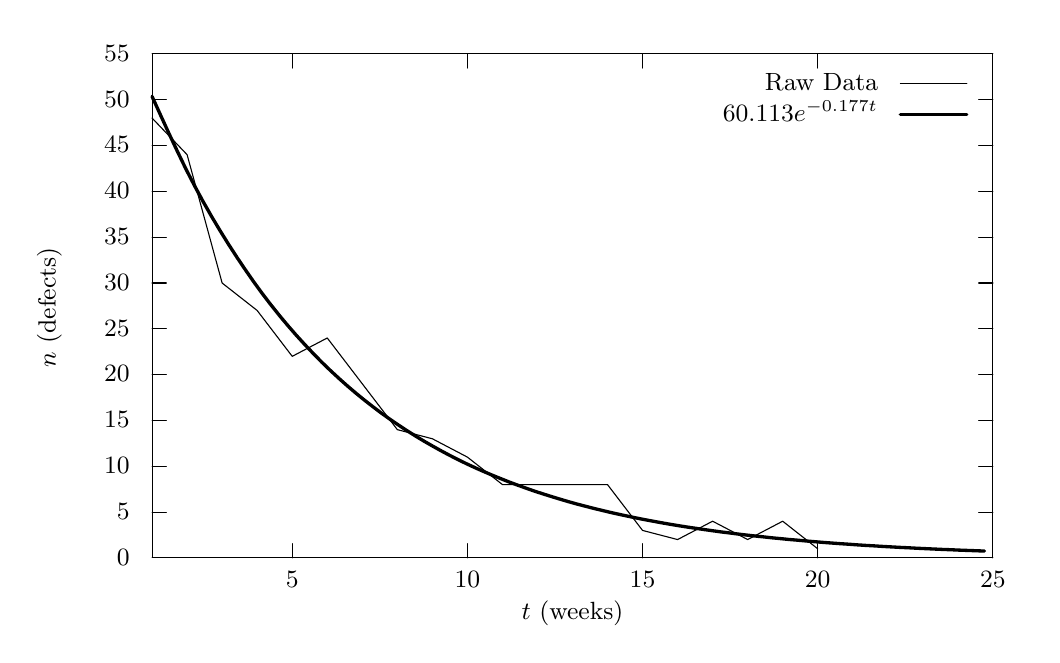
\begin{tikzpicture}[gnuplot]
%% generated with GNUPLOT 4.6p5 (Lua 5.2; terminal rev. 99, script rev. 100)
%% 2/09/2014 11:31:51 AM
\tikzset{every node/.append style={font={\fontsize{9pt}{10.8pt}\selectfont}}}
\gpmonochromelines
\path (0.000,0.000) rectangle (12.700,7.620);
\gpcolor{color=gp lt color border}
\gpsetlinetype{gp lt border}
\gpsetlinewidth{1.00}
\draw[gp path] (1.522,0.886)--(1.702,0.886);
\draw[gp path] (12.201,0.886)--(12.021,0.886);
\node[gp node right] at (1.356,0.886) { 0};
\draw[gp path] (1.522,1.468)--(1.702,1.468);
\draw[gp path] (12.201,1.468)--(12.021,1.468);
\node[gp node right] at (1.356,1.468) { 5};
\draw[gp path] (1.522,2.050)--(1.702,2.050);
\draw[gp path] (12.201,2.050)--(12.021,2.050);
\node[gp node right] at (1.356,2.050) { 10};
\draw[gp path] (1.522,2.632)--(1.702,2.632);
\draw[gp path] (12.201,2.632)--(12.021,2.632);
\node[gp node right] at (1.356,2.632) { 15};
\draw[gp path] (1.522,3.214)--(1.702,3.214);
\draw[gp path] (12.201,3.214)--(12.021,3.214);
\node[gp node right] at (1.356,3.214) { 20};
\draw[gp path] (1.522,3.796)--(1.702,3.796);
\draw[gp path] (12.201,3.796)--(12.021,3.796);
\node[gp node right] at (1.356,3.796) { 25};
\draw[gp path] (1.522,4.377)--(1.702,4.377);
\draw[gp path] (12.201,4.377)--(12.021,4.377);
\node[gp node right] at (1.356,4.377) { 30};
\draw[gp path] (1.522,4.959)--(1.702,4.959);
\draw[gp path] (12.201,4.959)--(12.021,4.959);
\node[gp node right] at (1.356,4.959) { 35};
\draw[gp path] (1.522,5.541)--(1.702,5.541);
\draw[gp path] (12.201,5.541)--(12.021,5.541);
\node[gp node right] at (1.356,5.541) { 40};
\draw[gp path] (1.522,6.123)--(1.702,6.123);
\draw[gp path] (12.201,6.123)--(12.021,6.123);
\node[gp node right] at (1.356,6.123) { 45};
\draw[gp path] (1.522,6.705)--(1.702,6.705);
\draw[gp path] (12.201,6.705)--(12.021,6.705);
\node[gp node right] at (1.356,6.705) { 50};
\draw[gp path] (1.522,7.287)--(1.702,7.287);
\draw[gp path] (12.201,7.287)--(12.021,7.287);
\node[gp node right] at (1.356,7.287) { 55};
\draw[gp path] (3.302,0.886)--(3.302,1.066);
\draw[gp path] (3.302,7.287)--(3.302,7.107);
\node[gp node center] at (3.302,0.609) { 5};
\draw[gp path] (5.527,0.886)--(5.527,1.066);
\draw[gp path] (5.527,7.287)--(5.527,7.107);
\node[gp node center] at (5.527,0.609) { 10};
\draw[gp path] (7.751,0.886)--(7.751,1.066);
\draw[gp path] (7.751,7.287)--(7.751,7.107);
\node[gp node center] at (7.751,0.609) { 15};
\draw[gp path] (9.976,0.886)--(9.976,1.066);
\draw[gp path] (9.976,7.287)--(9.976,7.107);
\node[gp node center] at (9.976,0.609) { 20};
\draw[gp path] (12.201,0.886)--(12.201,1.066);
\draw[gp path] (12.201,7.287)--(12.201,7.107);
\node[gp node center] at (12.201,0.609) { 25};
\draw[gp path] (1.522,7.287)--(1.522,0.886)--(12.201,0.886)--(12.201,7.287)--cycle;
\node[gp node center,rotate=-270] at (0.221,4.086) {$n$ (defects)};
\node[gp node center] at (6.861,0.194) {$t$ (weeks)};
\node[gp node right] at (10.859,6.911) {Raw Data};
\gpcolor{color=gp lt color 3}
\gpsetlinetype{gp lt plot 3}
\draw[gp path] (11.025,6.911)--(11.869,6.911);
\draw[gp path] (1.522,6.472)--(1.967,6.007)--(2.412,4.377)--(2.857,4.028)--(3.302,3.446)%
  --(3.747,3.679)--(4.192,3.097)--(4.637,2.515)--(5.082,2.399)--(5.527,2.166)--(5.972,1.817)%
  --(6.417,1.817)--(6.861,1.817)--(7.306,1.817)--(7.751,1.235)--(8.196,1.119)--(8.641,1.352)%
  --(9.086,1.119)--(9.531,1.352)--(9.976,1.002);
\gpcolor{color=gp lt color border}
\node[gp node right] at (10.859,6.518) {$60.113 e^{-0.177t}$};
\gpcolor{color=gp lt color 0}
\gpsetlinetype{gp lt plot 0}
\gpsetlinewidth{3.00}
\draw[gp path] (11.025,6.518)--(11.869,6.518);
\draw[gp path] (1.522,6.747)--(1.630,6.509)--(1.738,6.273)--(1.846,6.044)--(1.953,5.823)%
  --(2.061,5.613)--(2.169,5.414)--(2.277,5.224)--(2.385,5.043)--(2.493,4.869)--(2.601,4.702)%
  --(2.709,4.542)--(2.816,4.388)--(2.924,4.240)--(3.032,4.099)--(3.140,3.964)--(3.248,3.835)%
  --(3.356,3.711)--(3.464,3.593)--(3.572,3.479)--(3.679,3.370)--(3.787,3.266)--(3.895,3.166)%
  --(4.003,3.070)--(4.111,2.978)--(4.219,2.890)--(4.327,2.806)--(4.434,2.725)--(4.542,2.648)%
  --(4.650,2.574)--(4.758,2.503)--(4.866,2.435)--(4.974,2.370)--(5.082,2.308)--(5.190,2.248)%
  --(5.297,2.191)--(5.405,2.136)--(5.513,2.083)--(5.621,2.033)--(5.729,1.985)--(5.837,1.939)%
  --(5.945,1.895)--(6.052,1.852)--(6.160,1.812)--(6.268,1.773)--(6.376,1.735)--(6.484,1.700)%
  --(6.592,1.666)--(6.700,1.633)--(6.808,1.601)--(6.915,1.571)--(7.023,1.543)--(7.131,1.515)%
  --(7.239,1.489)--(7.347,1.463)--(7.455,1.439)--(7.563,1.416)--(7.671,1.393)--(7.778,1.372)%
  --(7.886,1.352)--(7.994,1.332)--(8.102,1.313)--(8.210,1.295)--(8.318,1.278)--(8.426,1.262)%
  --(8.533,1.246)--(8.641,1.231)--(8.749,1.216)--(8.857,1.203)--(8.965,1.189)--(9.073,1.176)%
  --(9.181,1.164)--(9.289,1.153)--(9.396,1.141)--(9.504,1.131)--(9.612,1.120)--(9.720,1.111)%
  --(9.828,1.101)--(9.936,1.092)--(10.044,1.083)--(10.151,1.075)--(10.259,1.067)--(10.367,1.060)%
  --(10.475,1.052)--(10.583,1.045)--(10.691,1.039)--(10.799,1.032)--(10.907,1.026)--(11.014,1.020)%
  --(11.122,1.015)--(11.230,1.009)--(11.338,1.004)--(11.446,0.999)--(11.554,0.994)--(11.662,0.990)%
  --(11.770,0.985)--(11.877,0.981)--(11.985,0.977)--(12.093,0.973);
\gpcolor{color=gp lt color border}
\gpsetlinetype{gp lt border}
\gpsetlinewidth{1.00}
\draw[gp path] (1.522,7.287)--(1.522,0.886)--(12.201,0.886)--(12.201,7.287)--cycle;
%% coordinates of the plot area
\gpdefrectangularnode{gp plot 1}{\pgfpoint{1.522cm}{0.886cm}}{\pgfpoint{12.201cm}{7.287cm}}
\end{tikzpicture}
%% gnuplot variables

  \caption{Exponential prediction vs. actual data}
  \label{defectdetection}
\end{figure}

\section{Metrics \& Strategies}
The interaction between metrics and strategies will be investigated to see how and why certain strategies cause certain metrics to differ. These variations will then be evaluated in terms of how those metrics affect the customer satisfaction vs the system reliability. Here we define a customer as being satisfied when the metric remains at a low level or trends downwards, or vice versa. The system is considered reliable with respect to a given strategy if that strategy would lead to little or no defects remaining in the software product at the end of the test and repair period ($t = 20$), and the strategy prioritises the most impactful issues.

Four metrics were chosen to be investigated, they were;
\begin{itemize}
 \item Ratio of defects fixed to defects found
 \item Total importance of found defects still to be fixed
 \item Average time in queue of major defects still to be fixed
 \item Estimate of number of unfixed defects still in the software
\end{itemize}

Six strategies of prioritising defect resolution were run against a model calculating the results of these metrics, they were;
\begin{itemize}
 \item Easy defects to hard defects, major defects to minor defects (i.e. Easy Major, Easy Minor, Hard Major, Hard Minor)
 \item Hard defects to easy defects, major defects to minor defects
 \item Major defects to minor defects, easy defects to hard defects (i.e. Easy Major, Hard Major, Easy Minor, Hard Minor)
 \item Minor defects to major defects, easy defects to hard defects
 \item Random ordering
 \item First in, first out ordering (e.g. oldest defect first)
\end{itemize}
  
\subsection{Ratio of defects fixed to defects found}
\begin{figure}
  \centering
  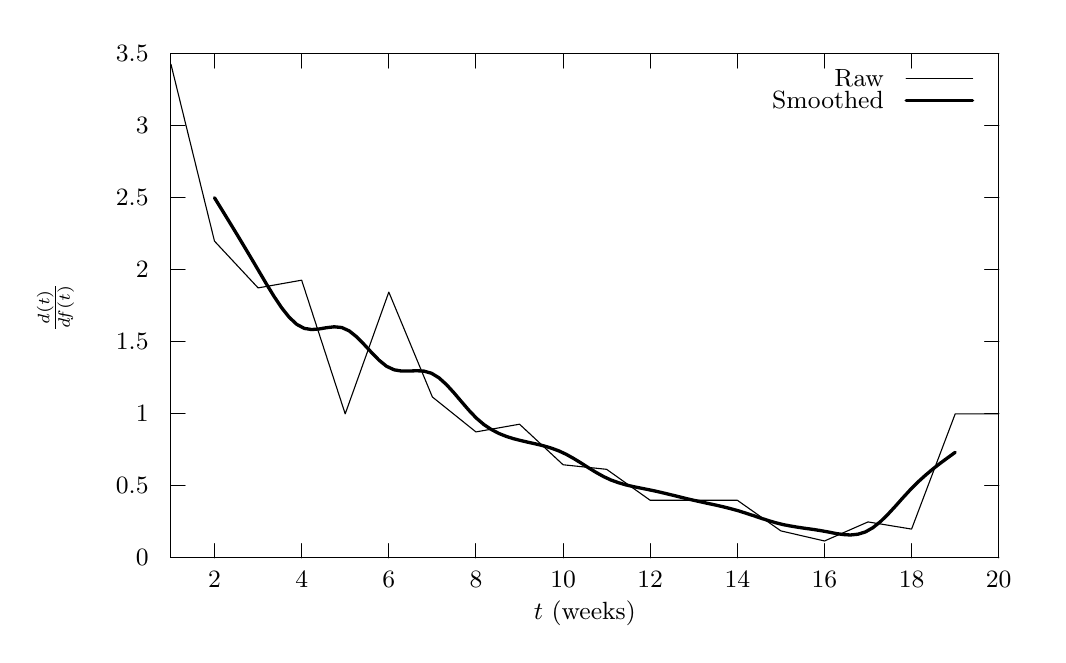
\begin{tikzpicture}[gnuplot]
%% generated with GNUPLOT 4.6p5 (Lua 5.2; terminal rev. 99, script rev. 100)
%% 2/09/2014 2:44:41 PM
\tikzset{every node/.append style={font={\fontsize{9pt}{10.8pt}\selectfont}}}
\gpmonochromelines
\path (0.000,0.000) rectangle (12.700,7.620);
\gpcolor{color=gp lt color border}
\gpsetlinetype{gp lt border}
\gpsetlinewidth{1.00}
\draw[gp path] (1.688,0.886)--(1.868,0.886);
\draw[gp path] (12.201,0.886)--(12.021,0.886);
\node[gp node right] at (1.522,0.886) { 0};
\draw[gp path] (1.688,1.800)--(1.868,1.800);
\draw[gp path] (12.201,1.800)--(12.021,1.800);
\node[gp node right] at (1.522,1.800) { 0.5};
\draw[gp path] (1.688,2.715)--(1.868,2.715);
\draw[gp path] (12.201,2.715)--(12.021,2.715);
\node[gp node right] at (1.522,2.715) { 1};
\draw[gp path] (1.688,3.629)--(1.868,3.629);
\draw[gp path] (12.201,3.629)--(12.021,3.629);
\node[gp node right] at (1.522,3.629) { 1.5};
\draw[gp path] (1.688,4.544)--(1.868,4.544);
\draw[gp path] (12.201,4.544)--(12.021,4.544);
\node[gp node right] at (1.522,4.544) { 2};
\draw[gp path] (1.688,5.458)--(1.868,5.458);
\draw[gp path] (12.201,5.458)--(12.021,5.458);
\node[gp node right] at (1.522,5.458) { 2.5};
\draw[gp path] (1.688,6.373)--(1.868,6.373);
\draw[gp path] (12.201,6.373)--(12.021,6.373);
\node[gp node right] at (1.522,6.373) { 3};
\draw[gp path] (1.688,7.287)--(1.868,7.287);
\draw[gp path] (12.201,7.287)--(12.021,7.287);
\node[gp node right] at (1.522,7.287) { 3.5};
\draw[gp path] (2.241,0.886)--(2.241,1.066);
\draw[gp path] (2.241,7.287)--(2.241,7.107);
\node[gp node center] at (2.241,0.609) { 2};
\draw[gp path] (3.348,0.886)--(3.348,1.066);
\draw[gp path] (3.348,7.287)--(3.348,7.107);
\node[gp node center] at (3.348,0.609) { 4};
\draw[gp path] (4.455,0.886)--(4.455,1.066);
\draw[gp path] (4.455,7.287)--(4.455,7.107);
\node[gp node center] at (4.455,0.609) { 6};
\draw[gp path] (5.561,0.886)--(5.561,1.066);
\draw[gp path] (5.561,7.287)--(5.561,7.107);
\node[gp node center] at (5.561,0.609) { 8};
\draw[gp path] (6.668,0.886)--(6.668,1.066);
\draw[gp path] (6.668,7.287)--(6.668,7.107);
\node[gp node center] at (6.668,0.609) { 10};
\draw[gp path] (7.774,0.886)--(7.774,1.066);
\draw[gp path] (7.774,7.287)--(7.774,7.107);
\node[gp node center] at (7.774,0.609) { 12};
\draw[gp path] (8.881,0.886)--(8.881,1.066);
\draw[gp path] (8.881,7.287)--(8.881,7.107);
\node[gp node center] at (8.881,0.609) { 14};
\draw[gp path] (9.988,0.886)--(9.988,1.066);
\draw[gp path] (9.988,7.287)--(9.988,7.107);
\node[gp node center] at (9.988,0.609) { 16};
\draw[gp path] (11.094,0.886)--(11.094,1.066);
\draw[gp path] (11.094,7.287)--(11.094,7.107);
\node[gp node center] at (11.094,0.609) { 18};
\draw[gp path] (12.201,0.886)--(12.201,1.066);
\draw[gp path] (12.201,7.287)--(12.201,7.107);
\node[gp node center] at (12.201,0.609) { 20};
\draw[gp path] (1.688,7.287)--(1.688,0.886)--(12.201,0.886)--(12.201,7.287)--cycle;
\node[gp node center,rotate=-270] at (0.221,4.086) {$\frac{d(t)}{df(t)}$};
\node[gp node center] at (6.944,0.194) {$t$ (weeks)};
\node[gp node right] at (10.859,6.969) {Raw};
\gpcolor{color=gp lt color 3}
\gpsetlinetype{gp lt plot 3}
\draw[gp path] (11.025,6.969)--(11.869,6.969);
\draw[gp path] (1.688,7.156)--(2.241,4.909)--(2.795,4.315)--(3.348,4.413)--(3.901,2.715)%
  --(4.455,4.262)--(5.008,2.930)--(5.561,2.486)--(6.115,2.584)--(6.668,2.069)--(7.221,2.011)%
  --(7.774,1.618)--(8.328,1.618)--(8.881,1.618)--(9.434,1.229)--(9.988,1.101)--(10.541,1.343)%
  --(11.094,1.252)--(11.648,2.715)--(12.201,2.715);
\gpcolor{color=gp lt color border}
\node[gp node right] at (10.859,6.692) {Smoothed};
\gpcolor{color=gp lt color 0}
\gpsetlinetype{gp lt plot 0}
\gpsetlinewidth{3.00}
\draw[gp path] (11.025,6.692)--(11.869,6.692);
\draw[gp path] (2.241,5.460)--(2.336,5.306)--(2.431,5.151)--(2.526,4.995)--(2.621,4.837)%
  --(2.716,4.678)--(2.811,4.517)--(2.906,4.356)--(3.001,4.201)--(3.096,4.060)--(3.191,3.941)%
  --(3.286,3.852)--(3.381,3.801)--(3.476,3.786)--(3.572,3.794)--(3.667,3.810)--(3.762,3.821)%
  --(3.857,3.812)--(3.952,3.769)--(4.047,3.693)--(4.142,3.596)--(4.237,3.493)--(4.332,3.396)%
  --(4.427,3.319)--(4.522,3.275)--(4.617,3.259)--(4.712,3.259)--(4.807,3.263)--(4.902,3.258)%
  --(4.997,3.231)--(5.092,3.173)--(5.187,3.087)--(5.282,2.983)--(5.377,2.871)--(5.472,2.761)%
  --(5.567,2.661)--(5.662,2.580)--(5.757,2.517)--(5.852,2.467)--(5.947,2.429)--(6.042,2.399)%
  --(6.137,2.375)--(6.232,2.353)--(6.327,2.332)--(6.422,2.309)--(6.517,2.281)--(6.612,2.246)%
  --(6.707,2.202)--(6.802,2.149)--(6.897,2.091)--(6.992,2.030)--(7.087,1.972)--(7.182,1.919)%
  --(7.277,1.875)--(7.372,1.841)--(7.467,1.813)--(7.562,1.791)--(7.657,1.772)--(7.752,1.753)%
  --(7.847,1.733)--(7.942,1.711)--(8.037,1.688)--(8.132,1.665)--(8.227,1.641)--(8.322,1.619)%
  --(8.417,1.598)--(8.512,1.577)--(8.607,1.557)--(8.702,1.535)--(8.797,1.511)--(8.892,1.485)%
  --(8.987,1.455)--(9.082,1.424)--(9.177,1.392)--(9.272,1.361)--(9.367,1.333)--(9.462,1.309)%
  --(9.557,1.291)--(9.652,1.275)--(9.747,1.261)--(9.842,1.248)--(9.937,1.233)--(10.032,1.216)%
  --(10.127,1.197)--(10.222,1.183)--(10.317,1.177)--(10.413,1.187)--(10.508,1.216)--(10.603,1.270)%
  --(10.698,1.346)--(10.793,1.439)--(10.888,1.542)--(10.983,1.649)--(11.078,1.752)--(11.173,1.848)%
  --(11.268,1.934)--(11.363,2.014)--(11.458,2.088)--(11.553,2.158)--(11.648,2.227);
\gpcolor{color=gp lt color border}
\gpsetlinetype{gp lt border}
\gpsetlinewidth{1.00}
\draw[gp path] (1.688,7.287)--(1.688,0.886)--(12.201,0.886)--(12.201,7.287)--cycle;
%% coordinates of the plot area
\gpdefrectangularnode{gp plot 1}{\pgfpoint{1.688cm}{0.886cm}}{\pgfpoint{12.201cm}{7.287cm}}
\end{tikzpicture}
%% gnuplot variables

  \caption{Ratio of defects fixed to defects found; aggregate results}
  \label{agg:dfdf}
\end{figure}

Figure \ref{agg:dfdf} (page \pageref{agg:dfdf}) shows the strategy results for the ratio of defects fixed to defects found. This was calculated as

$$\frac{d(t)}{\mathit{df}(t)}$$

Where $d(t)$ is the number of defects found in week $t$, and $\mathit{df}(t)$ is the number of defects fixed in week $t$.

As the graph shows, clearly the poorer strategy to minimise this metric in the beginning is ``Hard--Easy, Major--Minor''. This is due because by focusing on the most difficult defects with priority in the early weeks where many defects are being found, few are being fixed due to their difficulty, thus massively inflating the metric.

The ``Random'', ``FIFO'', ``Major-Minor, Easy--Hard'' and ``Minor--Major, Easy--Hard'' strategies sit in the middle of the best and worst strategies in the beginning, then become better than average at around weeks 8--10. This coincides with the massive drop-off of new defects being found around that point.

We see that the ``Major-Minor, Easy--Hard'' and ``Minor--Major, Easy--Hard'' have very different starting points, with ``Minor--Major'' starting at around 1.8 vs 3, however they converge around week 10. We can attribute this difference to the higher prevalence of minor defects vs major defects in the data set before that point; with more minor defects being present, and minor defects being more likely to be easy in this dataset, on average more bugs can be fixed per week in the early stages by preferring minor bugs.

The best strategy in the early term is clearly ``Easy--Hard, Major--Minor'', as this is the strategy that prioritises the easiest to fix defects, leading to a very high number of defects fixed per week.

Here we find that customer satisfaction is at odds with the system reliability, as this metric encourages the software development firm to underfind defects, as well as prioritise strategies for fixing that do not necessarily involve fixing the most important issues first, but rather the easiest ones.

\subsection{Total importance of found defects still to be fixed}
\begin{figure}
  \centering
  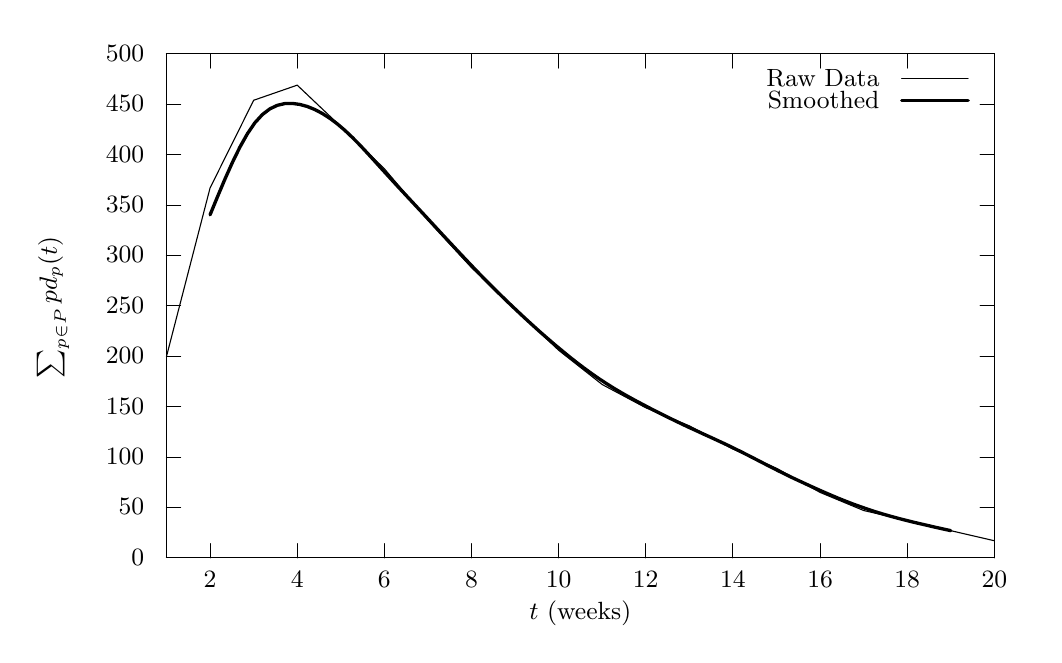
\begin{tikzpicture}[gnuplot]
%% generated with GNUPLOT 4.6p4 (Lua 5.1; terminal rev. 99, script rev. 100)
%% Thu 04 Sep 2014 10:50:27 WST
\tikzset{every node/.append style={font={\fontsize{9pt}{10.8pt}\selectfont}}}
\gpmonochromelines
\path (0.000,0.000) rectangle (12.700,7.620);
\gpcolor{color=gp lt color border}
\gpsetlinetype{gp lt border}
\gpsetlinewidth{1.00}
\draw[gp path] (1.688,0.886)--(1.868,0.886);
\draw[gp path] (12.201,0.886)--(12.021,0.886);
\node[gp node right] at (1.522,0.886) { 0};
\draw[gp path] (1.688,1.526)--(1.868,1.526);
\draw[gp path] (12.201,1.526)--(12.021,1.526);
\node[gp node right] at (1.522,1.526) { 50};
\draw[gp path] (1.688,2.166)--(1.868,2.166);
\draw[gp path] (12.201,2.166)--(12.021,2.166);
\node[gp node right] at (1.522,2.166) { 100};
\draw[gp path] (1.688,2.806)--(1.868,2.806);
\draw[gp path] (12.201,2.806)--(12.021,2.806);
\node[gp node right] at (1.522,2.806) { 150};
\draw[gp path] (1.688,3.446)--(1.868,3.446);
\draw[gp path] (12.201,3.446)--(12.021,3.446);
\node[gp node right] at (1.522,3.446) { 200};
\draw[gp path] (1.688,4.087)--(1.868,4.087);
\draw[gp path] (12.201,4.087)--(12.021,4.087);
\node[gp node right] at (1.522,4.087) { 250};
\draw[gp path] (1.688,4.727)--(1.868,4.727);
\draw[gp path] (12.201,4.727)--(12.021,4.727);
\node[gp node right] at (1.522,4.727) { 300};
\draw[gp path] (1.688,5.367)--(1.868,5.367);
\draw[gp path] (12.201,5.367)--(12.021,5.367);
\node[gp node right] at (1.522,5.367) { 350};
\draw[gp path] (1.688,6.007)--(1.868,6.007);
\draw[gp path] (12.201,6.007)--(12.021,6.007);
\node[gp node right] at (1.522,6.007) { 400};
\draw[gp path] (1.688,6.647)--(1.868,6.647);
\draw[gp path] (12.201,6.647)--(12.021,6.647);
\node[gp node right] at (1.522,6.647) { 450};
\draw[gp path] (1.688,7.287)--(1.868,7.287);
\draw[gp path] (12.201,7.287)--(12.021,7.287);
\node[gp node right] at (1.522,7.287) { 500};
\draw[gp path] (2.241,0.886)--(2.241,1.066);
\draw[gp path] (2.241,7.287)--(2.241,7.107);
\node[gp node center] at (2.241,0.609) { 2};
\draw[gp path] (3.348,0.886)--(3.348,1.066);
\draw[gp path] (3.348,7.287)--(3.348,7.107);
\node[gp node center] at (3.348,0.609) { 4};
\draw[gp path] (4.455,0.886)--(4.455,1.066);
\draw[gp path] (4.455,7.287)--(4.455,7.107);
\node[gp node center] at (4.455,0.609) { 6};
\draw[gp path] (5.561,0.886)--(5.561,1.066);
\draw[gp path] (5.561,7.287)--(5.561,7.107);
\node[gp node center] at (5.561,0.609) { 8};
\draw[gp path] (6.668,0.886)--(6.668,1.066);
\draw[gp path] (6.668,7.287)--(6.668,7.107);
\node[gp node center] at (6.668,0.609) { 10};
\draw[gp path] (7.774,0.886)--(7.774,1.066);
\draw[gp path] (7.774,7.287)--(7.774,7.107);
\node[gp node center] at (7.774,0.609) { 12};
\draw[gp path] (8.881,0.886)--(8.881,1.066);
\draw[gp path] (8.881,7.287)--(8.881,7.107);
\node[gp node center] at (8.881,0.609) { 14};
\draw[gp path] (9.988,0.886)--(9.988,1.066);
\draw[gp path] (9.988,7.287)--(9.988,7.107);
\node[gp node center] at (9.988,0.609) { 16};
\draw[gp path] (11.094,0.886)--(11.094,1.066);
\draw[gp path] (11.094,7.287)--(11.094,7.107);
\node[gp node center] at (11.094,0.609) { 18};
\draw[gp path] (12.201,0.886)--(12.201,1.066);
\draw[gp path] (12.201,7.287)--(12.201,7.107);
\node[gp node center] at (12.201,0.609) { 20};
\draw[gp path] (1.688,7.287)--(1.688,0.886)--(12.201,0.886)--(12.201,7.287)--cycle;
\node[gp node center,rotate=-270] at (0.221,4.086) {$\sum_{p \in P} p d_p(t)$};
\node[gp node center] at (6.944,0.194) {$t$ (weeks)};
\node[gp node right] at (10.859,6.969) {Raw Data};
\gpcolor{color=gp lt color 3}
\gpsetlinetype{gp lt plot 3}
\draw[gp path] (11.025,6.969)--(11.869,6.969);
\draw[gp path] (1.688,3.446)--(2.241,5.584)--(2.795,6.698)--(3.348,6.890)--(3.901,6.365)%
  --(4.455,5.828)--(5.008,5.175)--(5.561,4.573)--(6.115,4.048)--(6.668,3.523)--(7.221,3.088)%
  --(7.774,2.793)--(8.328,2.563)--(8.881,2.269)--(9.434,2.025)--(9.988,1.718)--(10.541,1.488)%
  --(11.094,1.360)--(11.648,1.232)--(12.201,1.104);
\gpcolor{color=gp lt color border}
\node[gp node right] at (10.859,6.692) {Smoothed};
\gpcolor{color=gp lt color 0}
\gpsetlinetype{gp lt plot 0}
\gpsetlinewidth{3.00}
\draw[gp path] (11.025,6.692)--(11.869,6.692);
\draw[gp path] (2.241,5.243)--(2.336,5.474)--(2.431,5.699)--(2.526,5.911)--(2.621,6.105)%
  --(2.716,6.274)--(2.811,6.413)--(2.906,6.517)--(3.001,6.589)--(3.096,6.634)--(3.191,6.656)%
  --(3.286,6.658)--(3.381,6.645)--(3.476,6.619)--(3.572,6.580)--(3.667,6.530)--(3.762,6.469)%
  --(3.857,6.398)--(3.952,6.317)--(4.047,6.227)--(4.142,6.131)--(4.237,6.029)--(4.332,5.925)%
  --(4.427,5.820)--(4.522,5.716)--(4.617,5.612)--(4.712,5.510)--(4.807,5.408)--(4.902,5.306)%
  --(4.997,5.204)--(5.092,5.101)--(5.187,4.998)--(5.282,4.896)--(5.377,4.794)--(5.472,4.693)%
  --(5.567,4.593)--(5.662,4.494)--(5.757,4.398)--(5.852,4.303)--(5.947,4.209)--(6.042,4.117)%
  --(6.137,4.027)--(6.232,3.938)--(6.327,3.851)--(6.422,3.765)--(6.517,3.682)--(6.612,3.600)%
  --(6.707,3.521)--(6.802,3.443)--(6.897,3.368)--(6.992,3.296)--(7.087,3.227)--(7.182,3.161)%
  --(7.277,3.099)--(7.372,3.039)--(7.467,2.983)--(7.562,2.929)--(7.657,2.877)--(7.752,2.827)%
  --(7.847,2.777)--(7.942,2.729)--(8.037,2.681)--(8.132,2.635)--(8.227,2.589)--(8.322,2.544)%
  --(8.417,2.501)--(8.512,2.457)--(8.607,2.414)--(8.702,2.370)--(8.797,2.326)--(8.892,2.280)%
  --(8.987,2.233)--(9.082,2.185)--(9.177,2.136)--(9.272,2.087)--(9.367,2.038)--(9.462,1.990)%
  --(9.557,1.943)--(9.652,1.897)--(9.747,1.853)--(9.842,1.809)--(9.937,1.766)--(10.032,1.724)%
  --(10.127,1.683)--(10.222,1.643)--(10.317,1.605)--(10.413,1.568)--(10.508,1.534)--(10.603,1.501)%
  --(10.698,1.470)--(10.793,1.441)--(10.888,1.414)--(10.983,1.388)--(11.078,1.364)--(11.173,1.340)%
  --(11.268,1.318)--(11.363,1.296)--(11.458,1.274)--(11.553,1.253)--(11.648,1.232);
\gpcolor{color=gp lt color border}
\gpsetlinetype{gp lt border}
\gpsetlinewidth{1.00}
\draw[gp path] (1.688,7.287)--(1.688,0.886)--(12.201,0.886)--(12.201,7.287)--cycle;
%% coordinates of the plot area
\gpdefrectangularnode{gp plot 1}{\pgfpoint{1.688cm}{0.886cm}}{\pgfpoint{12.201cm}{7.287cm}}
\end{tikzpicture}
%% gnuplot variables

  \caption{Total importance of found defects still to be fixed; aggregate results}
  \label{agg:tifd}
\end{figure}

Figure \ref{agg:tifd} (page \pageref{agg:tifd}) shows the strategy results for the total importance of found defects still to be fixed. This was calculated as

$$\sum_{p \in P} p d_p(t)$$

where $P$ is the set of importances of different priorities and $d_p(t)$ is the number of defects found of priority $p$ in week $t$.

This graph is more readily understood that the previous one, as the performance of each element on this graph can be explained as an optimisation of the most major defects that can be solved most quickly. The clear winner is ``Major--Minor, Easy--Hard'', as it ranks defects from the most important easiest to the least important hardest. A runner up is the similar ``Easy--Hard, Major--Minor'', however it fails to be most optimal by prioritising Hard Major over Easy Minor.

The worst result is the that of ``Minor--Major, Easy--Hard'', which effectively places major issues at the lowest priority of the set of strategies.

Customer satisfaction and this metric are closely related, as this metric closely maps with the resolution of the most important defects first, which will ultimately lead to less important bugs remaining in the final product. Similarly, system reliability with this approach will be maximised, as those issues which are most important are those which impact the system reliability the most.

\subsection{Average queue time of major defects still to be fixed}
\begin{figure}
  \centering
  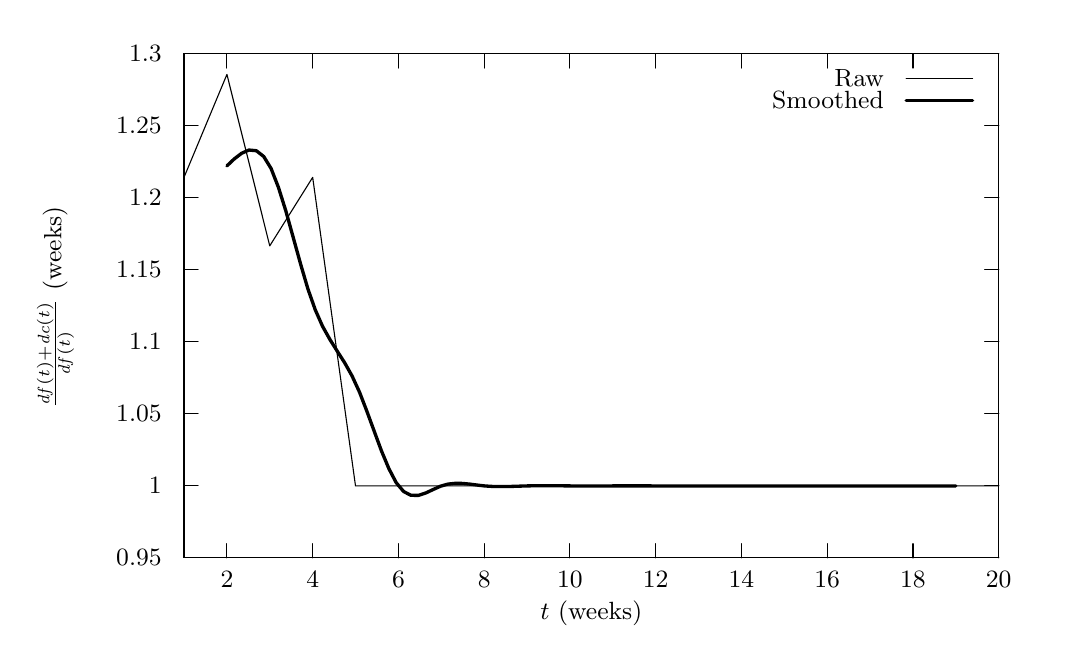
\begin{tikzpicture}[gnuplot]
%% generated with GNUPLOT 4.6p5 (Lua 5.2; terminal rev. 99, script rev. 100)
%% 2/09/2014 2:44:57 PM
\tikzset{every node/.append style={font={\fontsize{9pt}{10.8pt}\selectfont}}}
\gpmonochromelines
\path (0.000,0.000) rectangle (12.700,7.620);
\gpcolor{color=gp lt color border}
\gpsetlinetype{gp lt border}
\gpsetlinewidth{1.00}
\draw[gp path] (1.854,0.886)--(2.034,0.886);
\draw[gp path] (12.201,0.886)--(12.021,0.886);
\node[gp node right] at (1.688,0.886) { 0.95};
\draw[gp path] (1.854,1.800)--(2.034,1.800);
\draw[gp path] (12.201,1.800)--(12.021,1.800);
\node[gp node right] at (1.688,1.800) { 1};
\draw[gp path] (1.854,2.715)--(2.034,2.715);
\draw[gp path] (12.201,2.715)--(12.021,2.715);
\node[gp node right] at (1.688,2.715) { 1.05};
\draw[gp path] (1.854,3.629)--(2.034,3.629);
\draw[gp path] (12.201,3.629)--(12.021,3.629);
\node[gp node right] at (1.688,3.629) { 1.1};
\draw[gp path] (1.854,4.544)--(2.034,4.544);
\draw[gp path] (12.201,4.544)--(12.021,4.544);
\node[gp node right] at (1.688,4.544) { 1.15};
\draw[gp path] (1.854,5.458)--(2.034,5.458);
\draw[gp path] (12.201,5.458)--(12.021,5.458);
\node[gp node right] at (1.688,5.458) { 1.2};
\draw[gp path] (1.854,6.373)--(2.034,6.373);
\draw[gp path] (12.201,6.373)--(12.021,6.373);
\node[gp node right] at (1.688,6.373) { 1.25};
\draw[gp path] (1.854,7.287)--(2.034,7.287);
\draw[gp path] (12.201,7.287)--(12.021,7.287);
\node[gp node right] at (1.688,7.287) { 1.3};
\draw[gp path] (2.399,0.886)--(2.399,1.066);
\draw[gp path] (2.399,7.287)--(2.399,7.107);
\node[gp node center] at (2.399,0.609) { 2};
\draw[gp path] (3.488,0.886)--(3.488,1.066);
\draw[gp path] (3.488,7.287)--(3.488,7.107);
\node[gp node center] at (3.488,0.609) { 4};
\draw[gp path] (4.577,0.886)--(4.577,1.066);
\draw[gp path] (4.577,7.287)--(4.577,7.107);
\node[gp node center] at (4.577,0.609) { 6};
\draw[gp path] (5.666,0.886)--(5.666,1.066);
\draw[gp path] (5.666,7.287)--(5.666,7.107);
\node[gp node center] at (5.666,0.609) { 8};
\draw[gp path] (6.755,0.886)--(6.755,1.066);
\draw[gp path] (6.755,7.287)--(6.755,7.107);
\node[gp node center] at (6.755,0.609) { 10};
\draw[gp path] (7.844,0.886)--(7.844,1.066);
\draw[gp path] (7.844,7.287)--(7.844,7.107);
\node[gp node center] at (7.844,0.609) { 12};
\draw[gp path] (8.934,0.886)--(8.934,1.066);
\draw[gp path] (8.934,7.287)--(8.934,7.107);
\node[gp node center] at (8.934,0.609) { 14};
\draw[gp path] (10.023,0.886)--(10.023,1.066);
\draw[gp path] (10.023,7.287)--(10.023,7.107);
\node[gp node center] at (10.023,0.609) { 16};
\draw[gp path] (11.112,0.886)--(11.112,1.066);
\draw[gp path] (11.112,7.287)--(11.112,7.107);
\node[gp node center] at (11.112,0.609) { 18};
\draw[gp path] (12.201,0.886)--(12.201,1.066);
\draw[gp path] (12.201,7.287)--(12.201,7.107);
\node[gp node center] at (12.201,0.609) { 20};
\draw[gp path] (1.854,7.287)--(1.854,0.886)--(12.201,0.886)--(12.201,7.287)--cycle;
\node[gp node center,rotate=-270] at (0.221,4.086) {$\frac{\mathit{df}(t) + \mathit{dc}(t)}{\mathit{df}(t)}$ (weeks)};
\node[gp node center] at (7.027,0.194) {$t$ (weeks)};
\node[gp node right] at (10.859,6.969) {Raw};
\gpcolor{color=gp lt color 3}
\gpsetlinetype{gp lt plot 3}
\draw[gp path] (11.025,6.969)--(11.869,6.969);
\draw[gp path] (1.854,5.719)--(2.399,7.026)--(2.943,4.849)--(3.488,5.719)--(4.032,1.800)%
  --(4.577,1.800)--(5.121,1.800)--(5.666,1.800)--(6.211,1.800)--(6.755,1.800)--(7.300,1.800)%
  --(7.844,1.800)--(8.389,1.800)--(8.934,1.800)--(9.478,1.800)--(10.023,1.800)--(10.567,1.800)%
  --(11.656,1.800)--(12.201,1.800);
\gpcolor{color=gp lt color border}
\node[gp node right] at (10.859,6.692) {Smoothed};
\gpcolor{color=gp lt color 0}
\gpsetlinetype{gp lt plot 0}
\gpsetlinewidth{3.00}
\draw[gp path] (11.025,6.692)--(11.869,6.692);
\draw[gp path] (2.399,5.865)--(2.492,5.953)--(2.586,6.025)--(2.679,6.066)--(2.773,6.057)%
  --(2.866,5.984)--(2.960,5.831)--(3.053,5.592)--(3.147,5.293)--(3.240,4.959)--(3.334,4.620)%
  --(3.427,4.303)--(3.521,4.036)--(3.614,3.826)--(3.708,3.658)--(3.801,3.510)--(3.895,3.363)%
  --(3.988,3.197)--(4.082,2.993)--(4.175,2.752)--(4.269,2.496)--(4.362,2.244)--(4.456,2.019)%
  --(4.549,1.841)--(4.643,1.729)--(4.736,1.681)--(4.830,1.680)--(4.923,1.710)--(5.017,1.754)%
  --(5.110,1.796)--(5.204,1.823)--(5.297,1.833)--(5.391,1.832)--(5.485,1.823)--(5.578,1.811)%
  --(5.672,1.800)--(5.765,1.794)--(5.859,1.792)--(5.952,1.792)--(6.046,1.795)--(6.139,1.798)%
  --(6.233,1.801)--(6.326,1.802)--(6.420,1.803)--(6.513,1.802)--(6.607,1.802)--(6.700,1.801)%
  --(6.794,1.800)--(6.887,1.800)--(6.981,1.800)--(7.074,1.800)--(7.168,1.800)--(7.261,1.800)%
  --(7.355,1.801)--(7.448,1.801)--(7.542,1.801)--(7.635,1.801)--(7.729,1.801)--(7.822,1.800)%
  --(7.916,1.800)--(8.009,1.800)--(8.103,1.800)--(8.196,1.800)--(8.290,1.800)--(8.383,1.800)%
  --(8.477,1.800)--(8.570,1.800)--(8.664,1.800)--(8.758,1.800)--(8.851,1.800)--(8.945,1.800)%
  --(9.038,1.800)--(9.132,1.800)--(9.225,1.800)--(9.319,1.800)--(9.412,1.800)--(9.506,1.800)%
  --(9.599,1.800)--(9.693,1.800)--(9.786,1.800)--(9.880,1.800)--(9.973,1.800)--(10.067,1.800)%
  --(10.160,1.800)--(10.254,1.800)--(10.347,1.800)--(10.441,1.800)--(10.534,1.800)--(10.628,1.800)%
  --(10.721,1.800)--(10.815,1.800)--(10.908,1.800)--(11.002,1.800)--(11.095,1.800)--(11.189,1.800)%
  --(11.282,1.800)--(11.376,1.800)--(11.469,1.800)--(11.563,1.800)--(11.656,1.800);
\gpcolor{color=gp lt color border}
\gpsetlinetype{gp lt border}
\gpsetlinewidth{1.00}
\draw[gp path] (1.854,7.287)--(1.854,0.886)--(12.201,0.886)--(12.201,7.287)--cycle;
%% coordinates of the plot area
\gpdefrectangularnode{gp plot 1}{\pgfpoint{1.854cm}{0.886cm}}{\pgfpoint{12.201cm}{7.287cm}}
\end{tikzpicture}
%% gnuplot variables

  \caption{Average queue time of major defects still to be fixed; aggregate results}
  \label{agg:queuetime}
\end{figure}

\begin{figure}
  \centering
  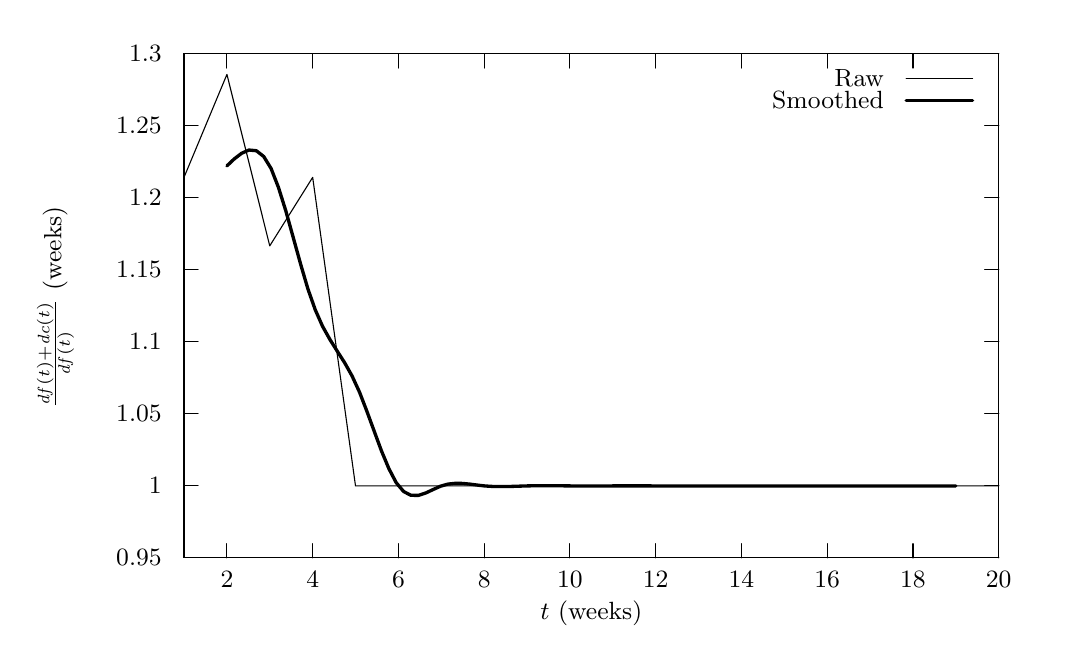
\begin{tikzpicture}[gnuplot]
%% generated with GNUPLOT 4.6p5 (Lua 5.2; terminal rev. 99, script rev. 100)
%% 2/09/2014 2:44:57 PM
\tikzset{every node/.append style={font={\fontsize{9pt}{10.8pt}\selectfont}}}
\gpmonochromelines
\path (0.000,0.000) rectangle (12.700,7.620);
\gpcolor{color=gp lt color border}
\gpsetlinetype{gp lt border}
\gpsetlinewidth{1.00}
\draw[gp path] (1.854,0.886)--(2.034,0.886);
\draw[gp path] (12.201,0.886)--(12.021,0.886);
\node[gp node right] at (1.688,0.886) { 0.95};
\draw[gp path] (1.854,1.800)--(2.034,1.800);
\draw[gp path] (12.201,1.800)--(12.021,1.800);
\node[gp node right] at (1.688,1.800) { 1};
\draw[gp path] (1.854,2.715)--(2.034,2.715);
\draw[gp path] (12.201,2.715)--(12.021,2.715);
\node[gp node right] at (1.688,2.715) { 1.05};
\draw[gp path] (1.854,3.629)--(2.034,3.629);
\draw[gp path] (12.201,3.629)--(12.021,3.629);
\node[gp node right] at (1.688,3.629) { 1.1};
\draw[gp path] (1.854,4.544)--(2.034,4.544);
\draw[gp path] (12.201,4.544)--(12.021,4.544);
\node[gp node right] at (1.688,4.544) { 1.15};
\draw[gp path] (1.854,5.458)--(2.034,5.458);
\draw[gp path] (12.201,5.458)--(12.021,5.458);
\node[gp node right] at (1.688,5.458) { 1.2};
\draw[gp path] (1.854,6.373)--(2.034,6.373);
\draw[gp path] (12.201,6.373)--(12.021,6.373);
\node[gp node right] at (1.688,6.373) { 1.25};
\draw[gp path] (1.854,7.287)--(2.034,7.287);
\draw[gp path] (12.201,7.287)--(12.021,7.287);
\node[gp node right] at (1.688,7.287) { 1.3};
\draw[gp path] (2.399,0.886)--(2.399,1.066);
\draw[gp path] (2.399,7.287)--(2.399,7.107);
\node[gp node center] at (2.399,0.609) { 2};
\draw[gp path] (3.488,0.886)--(3.488,1.066);
\draw[gp path] (3.488,7.287)--(3.488,7.107);
\node[gp node center] at (3.488,0.609) { 4};
\draw[gp path] (4.577,0.886)--(4.577,1.066);
\draw[gp path] (4.577,7.287)--(4.577,7.107);
\node[gp node center] at (4.577,0.609) { 6};
\draw[gp path] (5.666,0.886)--(5.666,1.066);
\draw[gp path] (5.666,7.287)--(5.666,7.107);
\node[gp node center] at (5.666,0.609) { 8};
\draw[gp path] (6.755,0.886)--(6.755,1.066);
\draw[gp path] (6.755,7.287)--(6.755,7.107);
\node[gp node center] at (6.755,0.609) { 10};
\draw[gp path] (7.844,0.886)--(7.844,1.066);
\draw[gp path] (7.844,7.287)--(7.844,7.107);
\node[gp node center] at (7.844,0.609) { 12};
\draw[gp path] (8.934,0.886)--(8.934,1.066);
\draw[gp path] (8.934,7.287)--(8.934,7.107);
\node[gp node center] at (8.934,0.609) { 14};
\draw[gp path] (10.023,0.886)--(10.023,1.066);
\draw[gp path] (10.023,7.287)--(10.023,7.107);
\node[gp node center] at (10.023,0.609) { 16};
\draw[gp path] (11.112,0.886)--(11.112,1.066);
\draw[gp path] (11.112,7.287)--(11.112,7.107);
\node[gp node center] at (11.112,0.609) { 18};
\draw[gp path] (12.201,0.886)--(12.201,1.066);
\draw[gp path] (12.201,7.287)--(12.201,7.107);
\node[gp node center] at (12.201,0.609) { 20};
\draw[gp path] (1.854,7.287)--(1.854,0.886)--(12.201,0.886)--(12.201,7.287)--cycle;
\node[gp node center,rotate=-270] at (0.221,4.086) {$\frac{\mathit{df}(t) + \mathit{dc}(t)}{\mathit{df}(t)}$ (weeks)};
\node[gp node center] at (7.027,0.194) {$t$ (weeks)};
\node[gp node right] at (10.859,6.969) {Raw};
\gpcolor{color=gp lt color 3}
\gpsetlinetype{gp lt plot 3}
\draw[gp path] (11.025,6.969)--(11.869,6.969);
\draw[gp path] (1.854,5.719)--(2.399,7.026)--(2.943,4.849)--(3.488,5.719)--(4.032,1.800)%
  --(4.577,1.800)--(5.121,1.800)--(5.666,1.800)--(6.211,1.800)--(6.755,1.800)--(7.300,1.800)%
  --(7.844,1.800)--(8.389,1.800)--(8.934,1.800)--(9.478,1.800)--(10.023,1.800)--(10.567,1.800)%
  --(11.656,1.800)--(12.201,1.800);
\gpcolor{color=gp lt color border}
\node[gp node right] at (10.859,6.692) {Smoothed};
\gpcolor{color=gp lt color 0}
\gpsetlinetype{gp lt plot 0}
\gpsetlinewidth{3.00}
\draw[gp path] (11.025,6.692)--(11.869,6.692);
\draw[gp path] (2.399,5.865)--(2.492,5.953)--(2.586,6.025)--(2.679,6.066)--(2.773,6.057)%
  --(2.866,5.984)--(2.960,5.831)--(3.053,5.592)--(3.147,5.293)--(3.240,4.959)--(3.334,4.620)%
  --(3.427,4.303)--(3.521,4.036)--(3.614,3.826)--(3.708,3.658)--(3.801,3.510)--(3.895,3.363)%
  --(3.988,3.197)--(4.082,2.993)--(4.175,2.752)--(4.269,2.496)--(4.362,2.244)--(4.456,2.019)%
  --(4.549,1.841)--(4.643,1.729)--(4.736,1.681)--(4.830,1.680)--(4.923,1.710)--(5.017,1.754)%
  --(5.110,1.796)--(5.204,1.823)--(5.297,1.833)--(5.391,1.832)--(5.485,1.823)--(5.578,1.811)%
  --(5.672,1.800)--(5.765,1.794)--(5.859,1.792)--(5.952,1.792)--(6.046,1.795)--(6.139,1.798)%
  --(6.233,1.801)--(6.326,1.802)--(6.420,1.803)--(6.513,1.802)--(6.607,1.802)--(6.700,1.801)%
  --(6.794,1.800)--(6.887,1.800)--(6.981,1.800)--(7.074,1.800)--(7.168,1.800)--(7.261,1.800)%
  --(7.355,1.801)--(7.448,1.801)--(7.542,1.801)--(7.635,1.801)--(7.729,1.801)--(7.822,1.800)%
  --(7.916,1.800)--(8.009,1.800)--(8.103,1.800)--(8.196,1.800)--(8.290,1.800)--(8.383,1.800)%
  --(8.477,1.800)--(8.570,1.800)--(8.664,1.800)--(8.758,1.800)--(8.851,1.800)--(8.945,1.800)%
  --(9.038,1.800)--(9.132,1.800)--(9.225,1.800)--(9.319,1.800)--(9.412,1.800)--(9.506,1.800)%
  --(9.599,1.800)--(9.693,1.800)--(9.786,1.800)--(9.880,1.800)--(9.973,1.800)--(10.067,1.800)%
  --(10.160,1.800)--(10.254,1.800)--(10.347,1.800)--(10.441,1.800)--(10.534,1.800)--(10.628,1.800)%
  --(10.721,1.800)--(10.815,1.800)--(10.908,1.800)--(11.002,1.800)--(11.095,1.800)--(11.189,1.800)%
  --(11.282,1.800)--(11.376,1.800)--(11.469,1.800)--(11.563,1.800)--(11.656,1.800);
\gpcolor{color=gp lt color border}
\gpsetlinetype{gp lt border}
\gpsetlinewidth{1.00}
\draw[gp path] (1.854,7.287)--(1.854,0.886)--(12.201,0.886)--(12.201,7.287)--cycle;
%% coordinates of the plot area
\gpdefrectangularnode{gp plot 1}{\pgfpoint{1.854cm}{0.886cm}}{\pgfpoint{12.201cm}{7.287cm}}
\end{tikzpicture}
%% gnuplot variables

  \caption{Average queue time of major defects still to be fixed; Minor--Major, Easy--Hard}
  \label{agg:queuetime:mmeh}
\end{figure}

Figure \ref{agg:queuetime} (page \pageref{agg:queuetime}) shows the strategy results for the average queue time of major defects still to be fixed. This is calculated as

$$\frac{\mathit{df}(t) + \mathit{dc}(t)}{\mathit{df}(t)}$$

where $\mathit{df}(t)$ is the number of defects fixed at week $t$ and $\mathit{dc}(t)$ is the total number of defects remaining unfixed from week 1 to week $t$.

The worst strategy ''Minor--Major, Easy--Hard``, which was cut off in figure \ref{agg:queuetime} due to its sheer size (it can be seen separately in figure \ref{agg:queuetime:mmeh} on page \pageref{agg:queuetime:mmeh}). It peaks of an average queue time of around 70 weeks, as it fully deprioritises major defects, which are the entire basis of this metric.

The best strategy is clearly ''Major--Minor, Easy--Hard``, as it prioritises the quickly fixable easy defects, which lead to a very low metric for the entire period.

Customer satisfaction and system reliability in this metric are closely related, as a strategy the customer is happy with would also promote system reliability. However, as the graphs show, all strategies converge around 1 week, demonstrating that all approaches would lead to major issues being fixed, but not necessarily with priority.

\subsection{Estimate of number of unfixed defects still in software}
\begin{figure}
  \centering
  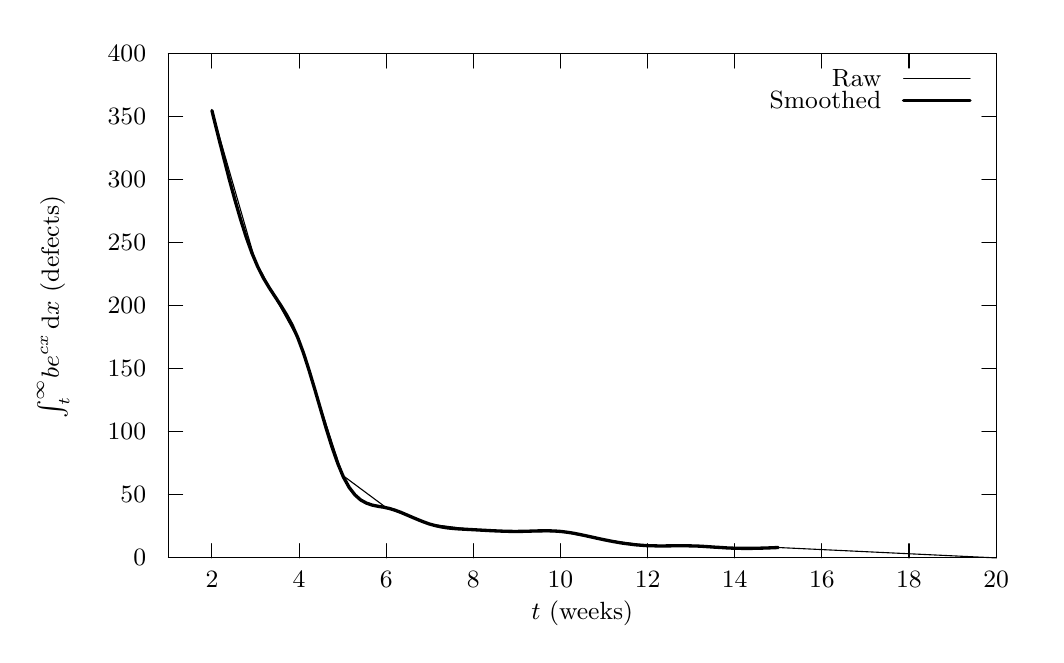
\begin{tikzpicture}[gnuplot]
%% generated with GNUPLOT 4.6p4 (Lua 5.1; terminal rev. 99, script rev. 100)
%% Thu 04 Sep 2014 10:50:27 WST
\tikzset{every node/.append style={font={\fontsize{9pt}{10.8pt}\selectfont}}}
\gpmonochromelines
\path (0.000,0.000) rectangle (12.700,7.620);
\gpcolor{color=gp lt color border}
\gpsetlinetype{gp lt border}
\gpsetlinewidth{1.00}
\draw[gp path] (1.688,0.886)--(1.868,0.886);
\draw[gp path] (12.201,0.886)--(12.021,0.886);
\node[gp node right] at (1.522,0.886) { 0};
\draw[gp path] (1.688,1.686)--(1.868,1.686);
\draw[gp path] (12.201,1.686)--(12.021,1.686);
\node[gp node right] at (1.522,1.686) { 50};
\draw[gp path] (1.688,2.486)--(1.868,2.486);
\draw[gp path] (12.201,2.486)--(12.021,2.486);
\node[gp node right] at (1.522,2.486) { 100};
\draw[gp path] (1.688,3.286)--(1.868,3.286);
\draw[gp path] (12.201,3.286)--(12.021,3.286);
\node[gp node right] at (1.522,3.286) { 150};
\draw[gp path] (1.688,4.087)--(1.868,4.087);
\draw[gp path] (12.201,4.087)--(12.021,4.087);
\node[gp node right] at (1.522,4.087) { 200};
\draw[gp path] (1.688,4.887)--(1.868,4.887);
\draw[gp path] (12.201,4.887)--(12.021,4.887);
\node[gp node right] at (1.522,4.887) { 250};
\draw[gp path] (1.688,5.687)--(1.868,5.687);
\draw[gp path] (12.201,5.687)--(12.021,5.687);
\node[gp node right] at (1.522,5.687) { 300};
\draw[gp path] (1.688,6.487)--(1.868,6.487);
\draw[gp path] (12.201,6.487)--(12.021,6.487);
\node[gp node right] at (1.522,6.487) { 350};
\draw[gp path] (1.688,7.287)--(1.868,7.287);
\draw[gp path] (12.201,7.287)--(12.021,7.287);
\node[gp node right] at (1.522,7.287) { 400};
\draw[gp path] (2.241,0.886)--(2.241,1.066);
\draw[gp path] (2.241,7.287)--(2.241,7.107);
\node[gp node center] at (2.241,0.609) { 2};
\draw[gp path] (3.348,0.886)--(3.348,1.066);
\draw[gp path] (3.348,7.287)--(3.348,7.107);
\node[gp node center] at (3.348,0.609) { 4};
\draw[gp path] (4.455,0.886)--(4.455,1.066);
\draw[gp path] (4.455,7.287)--(4.455,7.107);
\node[gp node center] at (4.455,0.609) { 6};
\draw[gp path] (5.561,0.886)--(5.561,1.066);
\draw[gp path] (5.561,7.287)--(5.561,7.107);
\node[gp node center] at (5.561,0.609) { 8};
\draw[gp path] (6.668,0.886)--(6.668,1.066);
\draw[gp path] (6.668,7.287)--(6.668,7.107);
\node[gp node center] at (6.668,0.609) { 10};
\draw[gp path] (7.774,0.886)--(7.774,1.066);
\draw[gp path] (7.774,7.287)--(7.774,7.107);
\node[gp node center] at (7.774,0.609) { 12};
\draw[gp path] (8.881,0.886)--(8.881,1.066);
\draw[gp path] (8.881,7.287)--(8.881,7.107);
\node[gp node center] at (8.881,0.609) { 14};
\draw[gp path] (9.988,0.886)--(9.988,1.066);
\draw[gp path] (9.988,7.287)--(9.988,7.107);
\node[gp node center] at (9.988,0.609) { 16};
\draw[gp path] (11.094,0.886)--(11.094,1.066);
\draw[gp path] (11.094,7.287)--(11.094,7.107);
\node[gp node center] at (11.094,0.609) { 18};
\draw[gp path] (12.201,0.886)--(12.201,1.066);
\draw[gp path] (12.201,7.287)--(12.201,7.107);
\node[gp node center] at (12.201,0.609) { 20};
\draw[gp path] (1.688,7.287)--(1.688,0.886)--(12.201,0.886)--(12.201,7.287)--cycle;
\node[gp node center,rotate=-270] at (0.221,4.086) {$\int_{t}^{\infty} \! be^{cx} \, \mathrm{d}x$ (defects)};
\node[gp node center] at (6.944,0.194) {$t$ (weeks)};
\node[gp node right] at (10.859,6.969) {Raw};
\gpcolor{color=gp lt color 3}
\gpsetlinetype{gp lt plot 3}
\draw[gp path] (11.025,6.969)--(11.869,6.969);
\draw[gp path] (2.241,6.568)--(2.795,4.647)--(3.348,3.642)--(3.901,1.935)--(4.455,1.524)%
  --(5.008,1.315)--(5.561,1.245)--(6.115,1.222)--(6.668,1.222)--(7.221,1.117)--(7.774,1.042)%
  --(8.328,1.039)--(8.881,1.009)--(9.434,1.018)--(12.201,0.886);
\gpcolor{color=gp lt color border}
\node[gp node right] at (10.859,6.692) {Smoothed};
\gpcolor{color=gp lt color 0}
\gpsetlinetype{gp lt plot 0}
\gpsetlinewidth{3.00}
\draw[gp path] (11.025,6.692)--(11.869,6.692);
\draw[gp path] (2.241,6.568)--(2.314,6.274)--(2.387,5.985)--(2.459,5.705)--(2.532,5.437)%
  --(2.605,5.187)--(2.677,4.959)--(2.750,4.756)--(2.823,4.584)--(2.895,4.441)--(2.968,4.319)%
  --(3.041,4.207)--(3.113,4.097)--(3.186,3.979)--(3.259,3.845)--(3.331,3.684)--(3.404,3.489)%
  --(3.476,3.265)--(3.549,3.022)--(3.622,2.772)--(3.694,2.525)--(3.767,2.292)--(3.840,2.084)%
  --(3.912,1.911)--(3.985,1.780)--(4.058,1.686)--(4.130,1.622)--(4.203,1.582)--(4.276,1.557)%
  --(4.348,1.542)--(4.421,1.530)--(4.494,1.514)--(4.566,1.492)--(4.639,1.465)--(4.712,1.434)%
  --(4.784,1.403)--(4.857,1.372)--(4.930,1.343)--(5.002,1.317)--(5.075,1.297)--(5.148,1.281)%
  --(5.220,1.269)--(5.293,1.261)--(5.366,1.255)--(5.438,1.251)--(5.511,1.247)--(5.584,1.243)%
  --(5.656,1.239)--(5.729,1.235)--(5.802,1.231)--(5.874,1.228)--(5.947,1.225)--(6.020,1.223)%
  --(6.092,1.222)--(6.165,1.223)--(6.237,1.224)--(6.310,1.227)--(6.383,1.229)--(6.455,1.230)%
  --(6.528,1.230)--(6.601,1.227)--(6.673,1.222)--(6.746,1.213)--(6.819,1.202)--(6.891,1.188)%
  --(6.964,1.173)--(7.037,1.157)--(7.109,1.141)--(7.182,1.125)--(7.255,1.110)--(7.327,1.096)%
  --(7.400,1.083)--(7.473,1.071)--(7.545,1.062)--(7.618,1.053)--(7.691,1.047)--(7.763,1.042)%
  --(7.836,1.040)--(7.909,1.038)--(7.981,1.038)--(8.054,1.039)--(8.127,1.040)--(8.199,1.040)%
  --(8.272,1.040)--(8.345,1.038)--(8.417,1.036)--(8.490,1.032)--(8.563,1.027)--(8.635,1.022)%
  --(8.708,1.018)--(8.781,1.013)--(8.853,1.010)--(8.926,1.008)--(8.998,1.007)--(9.071,1.007)%
  --(9.144,1.008)--(9.216,1.010)--(9.289,1.012)--(9.362,1.015)--(9.434,1.018);
\gpcolor{color=gp lt color border}
\gpsetlinetype{gp lt border}
\gpsetlinewidth{1.00}
\draw[gp path] (1.688,7.287)--(1.688,0.886)--(12.201,0.886)--(12.201,7.287)--cycle;
%% coordinates of the plot area
\gpdefrectangularnode{gp plot 1}{\pgfpoint{1.688cm}{0.886cm}}{\pgfpoint{12.201cm}{7.287cm}}
\end{tikzpicture}
%% gnuplot variables

  \caption{Estimate of number of unfixed defects still in software; aggregate results}
  \label{agg:remainingbugs}
\end{figure}

Figure \ref{agg:remainingbugs} (page \pageref{agg:remainingbugs}) shows the strategy results for the estimate of number of unfixed defects still in software, which were the same for every strategy explored. This result is calculated by performing a regression on $\{d(1), ..., d(t)\}$ for week $t$, to calculate values $b$ and $c$ for the exponential regression. Then the results of the integral

$$\int_{t}^{\infty} \! be^{cx} \, \mathrm{d}x$$

are calculated for each $t > 1$, then graphed. Because all previously mentioned strategies used the same allocation of $p_f = 1$, $p_r = 2$, this metric does not change within test strategies. See variants that differ from this and associated discussion in section \ref{defectminimisation}.

Customer satisfaction and system reliability are not discussed with this metric as there is no difference between scenarios.

\section{Employee Reallocations}
\label{defectminimisation}

To investigate how different metrics change with specifically tester/repairer variations, 3 variants of the ''Major--Minor, Easy--Hard`` were devised;

\begin{itemize}
  \item \textbf{Scenario A (Baseline)}: Major--Minor Easy--Hard priority
  
  \item \textbf{Scenario B}: $p_{f} = 2$, $p_{r} = 1$ for $1 \leq t \leq 4$, otherwise $p_{f} = 1$, $p_{r} = 2$
  
  \item \textbf{Scenario C}: $p_{f} = 0$, $p_{r} = 3$ if $t \bmod 3 = 0$, otherwise $p_{f} = 1$, $p_{r} = 2$
  
  \item \textbf{Scenario D}: $p_{f} = 2$, $p_{r} = 1$ for $1 \leq t \leq 4$, $p_{f} = 0$, $p_{r} = 3$ for $17 \leq t \leq 20$, otherwise $p_{f} = 1$, $p_{r} = 2$
  
\end{itemize}

Some data points with each of this scenarios could not be graphed due to limitations of exponential regression functions or division by zero errors. In the former case, affected datapoints have been excluded when at the end or beginning of the dataset, otherwise these points have been replaced by an average of adjacent points. In the latter case, affected formulas have been redefined as equation \ref{eq:dfdf} for the case of Defects Fixed:Defects Found and equation \ref{eq:queuetime} for average queuetime.

\begin{equation} \label{eq:dfdf}
\frac{d(t)+1}{\mathit{df}(t)+1}
\end{equation}

\begin{equation} \label{eq:queuetime}
\frac{\mathit{df}(t) + \mathit{dc}(t) + 1}{\mathit{df}(t) + 1}
\end{equation}

\begin{figure}
  \centering
  \begin{tikzpicture}[gnuplot]
%% generated with GNUPLOT 4.6p4 (Lua 5.1; terminal rev. 99, script rev. 100)
%% Sun 31 Aug 2014 10:54:04 WST
\tikzset{every node/.append style={font={\fontsize{9pt}{10.8pt}\selectfont}}}
\gpmonochromelines
\path (0.000,0.000) rectangle (12.700,7.620);
\gpcolor{color=gp lt color border}
\gpsetlinetype{gp lt border}
\gpsetlinewidth{1.00}
\draw[gp path] (1.688,0.886)--(1.868,0.886);
\draw[gp path] (12.201,0.886)--(12.021,0.886);
\node[gp node right] at (1.522,0.886) { 0};
\draw[gp path] (1.688,1.953)--(1.868,1.953);
\draw[gp path] (12.201,1.953)--(12.021,1.953);
\node[gp node right] at (1.522,1.953) { 0.5};
\draw[gp path] (1.688,3.020)--(1.868,3.020);
\draw[gp path] (12.201,3.020)--(12.021,3.020);
\node[gp node right] at (1.522,3.020) { 1};
\draw[gp path] (1.688,4.087)--(1.868,4.087);
\draw[gp path] (12.201,4.087)--(12.021,4.087);
\node[gp node right] at (1.522,4.087) { 1.5};
\draw[gp path] (1.688,5.153)--(1.868,5.153);
\draw[gp path] (12.201,5.153)--(12.021,5.153);
\node[gp node right] at (1.522,5.153) { 2};
\draw[gp path] (1.688,6.220)--(1.868,6.220);
\draw[gp path] (12.201,6.220)--(12.021,6.220);
\node[gp node right] at (1.522,6.220) { 2.5};
\draw[gp path] (1.688,7.287)--(1.868,7.287);
\draw[gp path] (12.201,7.287)--(12.021,7.287);
\node[gp node right] at (1.522,7.287) { 3};
\draw[gp path] (2.241,0.886)--(2.241,1.066);
\draw[gp path] (2.241,7.287)--(2.241,7.107);
\node[gp node center] at (2.241,0.609) { 2};
\draw[gp path] (3.348,0.886)--(3.348,1.066);
\draw[gp path] (3.348,7.287)--(3.348,7.107);
\node[gp node center] at (3.348,0.609) { 4};
\draw[gp path] (4.455,0.886)--(4.455,1.066);
\draw[gp path] (4.455,7.287)--(4.455,7.107);
\node[gp node center] at (4.455,0.609) { 6};
\draw[gp path] (5.561,0.886)--(5.561,1.066);
\draw[gp path] (5.561,7.287)--(5.561,7.107);
\node[gp node center] at (5.561,0.609) { 8};
\draw[gp path] (6.668,0.886)--(6.668,1.066);
\draw[gp path] (6.668,7.287)--(6.668,7.107);
\node[gp node center] at (6.668,0.609) { 10};
\draw[gp path] (7.774,0.886)--(7.774,1.066);
\draw[gp path] (7.774,7.287)--(7.774,7.107);
\node[gp node center] at (7.774,0.609) { 12};
\draw[gp path] (8.881,0.886)--(8.881,1.066);
\draw[gp path] (8.881,7.287)--(8.881,7.107);
\node[gp node center] at (8.881,0.609) { 14};
\draw[gp path] (9.988,0.886)--(9.988,1.066);
\draw[gp path] (9.988,7.287)--(9.988,7.107);
\node[gp node center] at (9.988,0.609) { 16};
\draw[gp path] (11.094,0.886)--(11.094,1.066);
\draw[gp path] (11.094,7.287)--(11.094,7.107);
\node[gp node center] at (11.094,0.609) { 18};
\draw[gp path] (12.201,0.886)--(12.201,1.066);
\draw[gp path] (12.201,7.287)--(12.201,7.107);
\node[gp node center] at (12.201,0.609) { 20};
\draw[gp path] (1.688,7.287)--(1.688,0.886)--(12.201,0.886)--(12.201,7.287)--cycle;
\node[gp node center,rotate=-270] at (0.221,4.086) {$r$};
\node[gp node center] at (6.944,0.194) {$t$ (weeks)};
\node[gp node right] at (10.859,6.969) {Modified};
\gpcolor{color=gp lt color 0}
\gpsetlinetype{gp lt plot 0}
\gpsetlinewidth{3.00}
\draw[gp path] (11.025,6.969)--(11.869,6.969);
\draw[gp path] (2.241,5.280)--(2.303,5.154)--(2.364,5.029)--(2.426,4.903)--(2.487,4.779)%
  --(2.549,4.655)--(2.610,4.533)--(2.672,4.412)--(2.733,4.293)--(2.795,4.175)--(2.856,4.060)%
  --(2.918,3.949)--(2.979,3.844)--(3.041,3.745)--(3.102,3.656)--(3.164,3.577)--(3.225,3.510)%
  --(3.286,3.457)--(3.348,3.420)--(3.409,3.399)--(3.471,3.391)--(3.532,3.394)--(3.594,3.403)%
  --(3.655,3.415)--(3.717,3.426)--(3.778,3.433)--(3.840,3.432)--(3.901,3.420)--(3.963,3.393)%
  --(4.024,3.354)--(4.086,3.304)--(4.147,3.245)--(4.209,3.181)--(4.270,3.113)--(4.332,3.044)%
  --(4.393,2.975)--(4.455,2.910)--(4.516,2.849)--(4.578,2.794)--(4.639,2.744)--(4.700,2.700)%
  --(4.762,2.662)--(4.823,2.629)--(4.885,2.601)--(4.946,2.579)--(5.008,2.563)--(5.069,2.552)%
  --(5.131,2.547)--(5.192,2.545)--(5.254,2.546)--(5.315,2.549)--(5.377,2.553)--(5.438,2.557)%
  --(5.500,2.561)--(5.561,2.563)--(5.623,2.563)--(5.684,2.560)--(5.746,2.554)--(5.807,2.545)%
  --(5.869,2.533)--(5.930,2.518)--(5.992,2.499)--(6.053,2.477)--(6.115,2.451)--(6.176,2.421)%
  --(6.237,2.389)--(6.299,2.355)--(6.360,2.320)--(6.422,2.287)--(6.483,2.255)--(6.545,2.226)%
  --(6.606,2.202)--(6.668,2.183)--(6.729,2.170)--(6.791,2.163)--(6.852,2.160)--(6.914,2.160)%
  --(6.975,2.164)--(7.037,2.169)--(7.098,2.174)--(7.160,2.179)--(7.221,2.183)--(7.283,2.185)%
  --(7.344,2.184)--(7.406,2.183)--(7.467,2.181)--(7.529,2.179)--(7.590,2.178)--(7.652,2.178)%
  --(7.713,2.179)--(7.774,2.183)--(7.836,2.190)--(7.897,2.199)--(7.959,2.210)--(8.020,2.224)%
  --(8.082,2.239)--(8.143,2.255)--(8.205,2.272)--(8.266,2.290)--(8.328,2.308);
\gpcolor{color=gp lt color border}
\node[gp node right] at (10.859,6.692) {Baseline};
\gpcolor{color=gp lt color 3}
\gpsetlinetype{gp lt plot 3}
\gpsetlinewidth{1.00}
\draw[gp path] (11.025,6.692)--(11.869,6.692);
\draw[gp path] (2.241,6.922)--(2.336,6.702)--(2.431,6.484)--(2.526,6.269)--(2.621,6.057)%
  --(2.716,5.850)--(2.811,5.648)--(2.906,5.454)--(3.001,5.267)--(3.096,5.087)--(3.191,4.915)%
  --(3.286,4.750)--(3.381,4.594)--(3.476,4.445)--(3.572,4.303)--(3.667,4.169)--(3.762,4.040)%
  --(3.857,3.916)--(3.952,3.798)--(4.047,3.684)--(4.142,3.574)--(4.237,3.470)--(4.332,3.370)%
  --(4.427,3.274)--(4.522,3.184)--(4.617,3.098)--(4.712,3.015)--(4.807,2.933)--(4.902,2.852)%
  --(4.997,2.770)--(5.092,2.686)--(5.187,2.601)--(5.282,2.519)--(5.377,2.441)--(5.472,2.369)%
  --(5.567,2.305)--(5.662,2.251)--(5.757,2.206)--(5.852,2.167)--(5.947,2.133)--(6.042,2.101)%
  --(6.137,2.069)--(6.232,2.036)--(6.327,2.003)--(6.422,1.971)--(6.517,1.939)--(6.612,1.908)%
  --(6.707,1.880)--(6.802,1.854)--(6.897,1.831)--(6.992,1.813)--(7.087,1.799)--(7.182,1.790)%
  --(7.277,1.787)--(7.372,1.790)--(7.467,1.800)--(7.562,1.815)--(7.657,1.836)--(7.752,1.863)%
  --(7.847,1.896)--(7.942,1.933)--(8.037,1.971)--(8.132,2.007)--(8.227,2.037)--(8.322,2.060)%
  --(8.417,2.072)--(8.512,2.072)--(8.607,2.062)--(8.702,2.041)--(8.797,2.010)--(8.892,1.969)%
  --(8.987,1.919)--(9.082,1.864)--(9.177,1.806)--(9.272,1.749)--(9.367,1.698)--(9.462,1.655)%
  --(9.557,1.621)--(9.652,1.595)--(9.747,1.573)--(9.842,1.551)--(9.937,1.528)--(10.032,1.499)%
  --(10.127,1.467)--(10.222,1.438)--(10.317,1.420)--(10.413,1.419)--(10.508,1.442)--(10.603,1.496)%
  --(10.698,1.579)--(10.793,1.680)--(10.888,1.794)--(10.983,1.910)--(11.078,2.021)--(11.173,2.120)%
  --(11.268,2.205)--(11.363,2.279)--(11.458,2.346)--(11.553,2.408)--(11.648,2.466);
\gpcolor{color=gp lt color border}
\gpsetlinetype{gp lt border}
\draw[gp path] (1.688,7.287)--(1.688,0.886)--(12.201,0.886)--(12.201,7.287)--cycle;
%% coordinates of the plot area
\gpdefrectangularnode{gp plot 1}{\pgfpoint{1.688cm}{0.886cm}}{\pgfpoint{12.201cm}{7.287cm}}
\end{tikzpicture}
%% gnuplot variables

  \caption{Ratio of defects fixed to defects found; comparison}
  \label{comp:dfdf}
\end{figure}

\begin{figure}
  \centering
  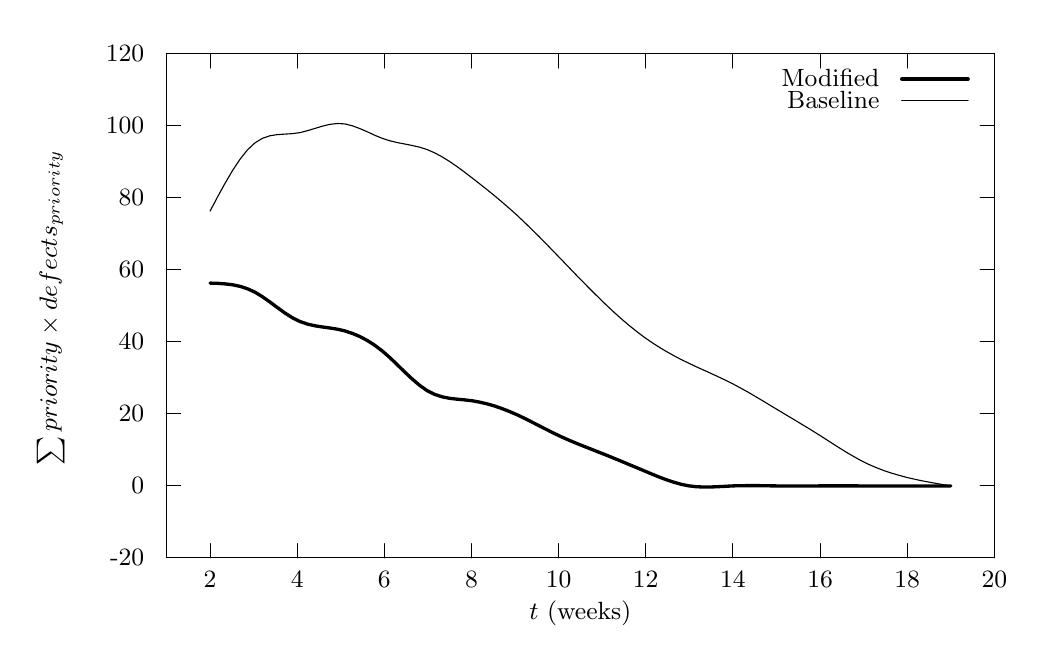
\begin{tikzpicture}[gnuplot]
%% generated with GNUPLOT 4.6p4 (Lua 5.1; terminal rev. 99, script rev. 100)
%% Sun 31 Aug 2014 10:54:04 WST
\tikzset{every node/.append style={font={\fontsize{9pt}{10.8pt}\selectfont}}}
\gpmonochromelines
\path (0.000,0.000) rectangle (12.700,7.620);
\gpcolor{color=gp lt color border}
\gpsetlinetype{gp lt border}
\gpsetlinewidth{1.00}
\draw[gp path] (1.688,0.886)--(1.868,0.886);
\draw[gp path] (12.201,0.886)--(12.021,0.886);
\node[gp node right] at (1.522,0.886) {-20};
\draw[gp path] (1.688,1.800)--(1.868,1.800);
\draw[gp path] (12.201,1.800)--(12.021,1.800);
\node[gp node right] at (1.522,1.800) { 0};
\draw[gp path] (1.688,2.715)--(1.868,2.715);
\draw[gp path] (12.201,2.715)--(12.021,2.715);
\node[gp node right] at (1.522,2.715) { 20};
\draw[gp path] (1.688,3.629)--(1.868,3.629);
\draw[gp path] (12.201,3.629)--(12.021,3.629);
\node[gp node right] at (1.522,3.629) { 40};
\draw[gp path] (1.688,4.544)--(1.868,4.544);
\draw[gp path] (12.201,4.544)--(12.021,4.544);
\node[gp node right] at (1.522,4.544) { 60};
\draw[gp path] (1.688,5.458)--(1.868,5.458);
\draw[gp path] (12.201,5.458)--(12.021,5.458);
\node[gp node right] at (1.522,5.458) { 80};
\draw[gp path] (1.688,6.373)--(1.868,6.373);
\draw[gp path] (12.201,6.373)--(12.021,6.373);
\node[gp node right] at (1.522,6.373) { 100};
\draw[gp path] (1.688,7.287)--(1.868,7.287);
\draw[gp path] (12.201,7.287)--(12.021,7.287);
\node[gp node right] at (1.522,7.287) { 120};
\draw[gp path] (2.241,0.886)--(2.241,1.066);
\draw[gp path] (2.241,7.287)--(2.241,7.107);
\node[gp node center] at (2.241,0.609) { 2};
\draw[gp path] (3.348,0.886)--(3.348,1.066);
\draw[gp path] (3.348,7.287)--(3.348,7.107);
\node[gp node center] at (3.348,0.609) { 4};
\draw[gp path] (4.455,0.886)--(4.455,1.066);
\draw[gp path] (4.455,7.287)--(4.455,7.107);
\node[gp node center] at (4.455,0.609) { 6};
\draw[gp path] (5.561,0.886)--(5.561,1.066);
\draw[gp path] (5.561,7.287)--(5.561,7.107);
\node[gp node center] at (5.561,0.609) { 8};
\draw[gp path] (6.668,0.886)--(6.668,1.066);
\draw[gp path] (6.668,7.287)--(6.668,7.107);
\node[gp node center] at (6.668,0.609) { 10};
\draw[gp path] (7.774,0.886)--(7.774,1.066);
\draw[gp path] (7.774,7.287)--(7.774,7.107);
\node[gp node center] at (7.774,0.609) { 12};
\draw[gp path] (8.881,0.886)--(8.881,1.066);
\draw[gp path] (8.881,7.287)--(8.881,7.107);
\node[gp node center] at (8.881,0.609) { 14};
\draw[gp path] (9.988,0.886)--(9.988,1.066);
\draw[gp path] (9.988,7.287)--(9.988,7.107);
\node[gp node center] at (9.988,0.609) { 16};
\draw[gp path] (11.094,0.886)--(11.094,1.066);
\draw[gp path] (11.094,7.287)--(11.094,7.107);
\node[gp node center] at (11.094,0.609) { 18};
\draw[gp path] (12.201,0.886)--(12.201,1.066);
\draw[gp path] (12.201,7.287)--(12.201,7.107);
\node[gp node center] at (12.201,0.609) { 20};
\draw[gp path] (1.688,7.287)--(1.688,0.886)--(12.201,0.886)--(12.201,7.287)--cycle;
\node[gp node center,rotate=-270] at (0.221,4.086) {$\sum priority \times defects_{priority}$};
\node[gp node center] at (6.944,0.194) {$t$ (weeks)};
\node[gp node right] at (10.859,6.969) {Modified};
\gpcolor{color=gp lt color 0}
\gpsetlinetype{gp lt plot 0}
\gpsetlinewidth{3.00}
\draw[gp path] (11.025,6.969)--(11.869,6.969);
\draw[gp path] (2.241,4.376)--(2.336,4.373)--(2.431,4.366)--(2.526,4.355)--(2.621,4.335)%
  --(2.716,4.304)--(2.811,4.261)--(2.906,4.203)--(3.001,4.136)--(3.096,4.065)--(3.191,3.997)%
  --(3.286,3.936)--(3.381,3.889)--(3.476,3.856)--(3.572,3.834)--(3.667,3.819)--(3.762,3.806)%
  --(3.857,3.791)--(3.952,3.769)--(4.047,3.738)--(4.142,3.698)--(4.237,3.648)--(4.332,3.587)%
  --(4.427,3.515)--(4.522,3.432)--(4.617,3.341)--(4.712,3.248)--(4.807,3.159)--(4.902,3.078)%
  --(4.997,3.011)--(5.092,2.963)--(5.187,2.932)--(5.282,2.913)--(5.377,2.902)--(5.472,2.893)%
  --(5.567,2.882)--(5.662,2.865)--(5.757,2.843)--(5.852,2.816)--(5.947,2.783)--(6.042,2.746)%
  --(6.137,2.705)--(6.232,2.660)--(6.327,2.612)--(6.422,2.563)--(6.517,2.515)--(6.612,2.467)%
  --(6.707,2.422)--(6.802,2.380)--(6.897,2.340)--(6.992,2.302)--(7.087,2.265)--(7.182,2.227)%
  --(7.277,2.190)--(7.372,2.151)--(7.467,2.112)--(7.562,2.072)--(7.657,2.033)--(7.752,1.993)%
  --(7.847,1.953)--(7.942,1.914)--(8.037,1.878)--(8.132,1.847)--(8.227,1.820)--(8.322,1.801)%
  --(8.417,1.790)--(8.512,1.786)--(8.607,1.787)--(8.702,1.791)--(8.797,1.796)--(8.892,1.801)%
  --(8.987,1.803)--(9.082,1.804)--(9.177,1.804)--(9.272,1.803)--(9.367,1.801)--(9.462,1.800)%
  --(9.557,1.800)--(9.652,1.799)--(9.747,1.800)--(9.842,1.800)--(9.937,1.800)--(10.032,1.801)%
  --(10.127,1.801)--(10.222,1.801)--(10.317,1.801)--(10.413,1.801)--(10.508,1.800)--(10.603,1.800)%
  --(10.698,1.800)--(10.793,1.800)--(10.888,1.800)--(10.983,1.800)--(11.078,1.800)--(11.173,1.800)%
  --(11.268,1.800)--(11.363,1.800)--(11.458,1.800)--(11.553,1.800)--(11.648,1.800);
\gpcolor{color=gp lt color border}
\node[gp node right] at (10.859,6.692) {Baseline};
\gpcolor{color=gp lt color 3}
\gpsetlinetype{gp lt plot 3}
\gpsetlinewidth{1.00}
\draw[gp path] (11.025,6.692)--(11.869,6.692);
\draw[gp path] (2.241,5.290)--(2.336,5.470)--(2.431,5.643)--(2.526,5.805)--(2.621,5.948)%
  --(2.716,6.068)--(2.811,6.157)--(2.906,6.215)--(3.001,6.247)--(3.096,6.262)--(3.191,6.268)%
  --(3.286,6.274)--(3.381,6.287)--(3.476,6.311)--(3.572,6.340)--(3.667,6.369)--(3.762,6.392)%
  --(3.857,6.403)--(3.952,6.398)--(4.047,6.374)--(4.142,6.339)--(4.237,6.298)--(4.332,6.254)%
  --(4.427,6.215)--(4.522,6.184)--(4.617,6.161)--(4.712,6.143)--(4.807,6.124)--(4.902,6.102)%
  --(4.997,6.072)--(5.092,6.031)--(5.187,5.980)--(5.282,5.921)--(5.377,5.856)--(5.472,5.786)%
  --(5.567,5.713)--(5.662,5.639)--(5.757,5.564)--(5.852,5.487)--(5.947,5.407)--(6.042,5.325)%
  --(6.137,5.240)--(6.232,5.150)--(6.327,5.058)--(6.422,4.964)--(6.517,4.867)--(6.612,4.769)%
  --(6.707,4.671)--(6.802,4.572)--(6.897,4.473)--(6.992,4.376)--(7.087,4.280)--(7.182,4.186)%
  --(7.277,4.094)--(7.372,4.005)--(7.467,3.920)--(7.562,3.839)--(7.657,3.763)--(7.752,3.691)%
  --(7.847,3.625)--(7.942,3.564)--(8.037,3.507)--(8.132,3.454)--(8.227,3.404)--(8.322,3.358)%
  --(8.417,3.313)--(8.512,3.270)--(8.607,3.227)--(8.702,3.183)--(8.797,3.138)--(8.892,3.090)%
  --(8.987,3.039)--(9.082,2.986)--(9.177,2.930)--(9.272,2.874)--(9.367,2.816)--(9.462,2.759)%
  --(9.557,2.702)--(9.652,2.646)--(9.747,2.588)--(9.842,2.531)--(9.937,2.472)--(10.032,2.412)%
  --(10.127,2.351)--(10.222,2.290)--(10.317,2.231)--(10.413,2.175)--(10.508,2.122)--(10.603,2.075)%
  --(10.698,2.034)--(10.793,1.997)--(10.888,1.965)--(10.983,1.937)--(11.078,1.911)--(11.173,1.889)%
  --(11.268,1.868)--(11.363,1.850)--(11.458,1.833)--(11.553,1.816)--(11.648,1.800);
\gpcolor{color=gp lt color border}
\gpsetlinetype{gp lt border}
\draw[gp path] (1.688,7.287)--(1.688,0.886)--(12.201,0.886)--(12.201,7.287)--cycle;
%% coordinates of the plot area
\gpdefrectangularnode{gp plot 1}{\pgfpoint{1.688cm}{0.886cm}}{\pgfpoint{12.201cm}{7.287cm}}
\end{tikzpicture}
%% gnuplot variables

  \caption{Total importance of found defects still to be fixed; comparison}
  \label{comp:tifd}
\end{figure}

\begin{figure}
  \centering
  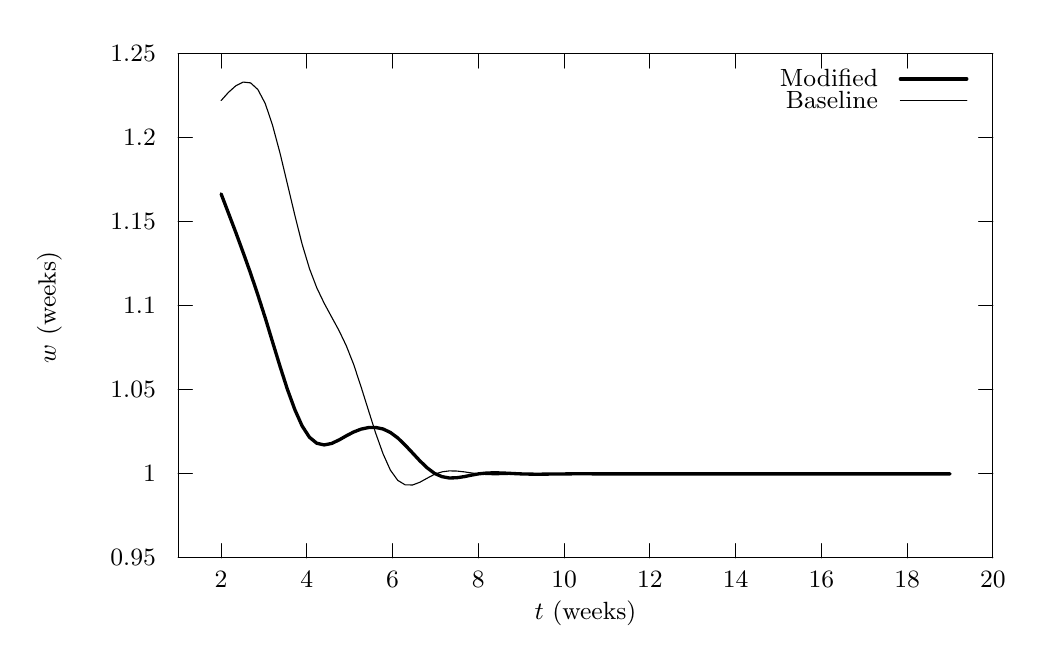
\begin{tikzpicture}[gnuplot]
%% generated with GNUPLOT 4.6p4 (Lua 5.1; terminal rev. 99, script rev. 100)
%% Sun 31 Aug 2014 10:54:04 WST
\tikzset{every node/.append style={font={\fontsize{9pt}{10.8pt}\selectfont}}}
\gpmonochromelines
\path (0.000,0.000) rectangle (12.700,7.620);
\gpcolor{color=gp lt color border}
\gpsetlinetype{gp lt border}
\gpsetlinewidth{1.00}
\draw[gp path] (1.854,0.886)--(2.034,0.886);
\draw[gp path] (12.201,0.886)--(12.021,0.886);
\node[gp node right] at (1.688,0.886) { 0.95};
\draw[gp path] (1.854,1.953)--(2.034,1.953);
\draw[gp path] (12.201,1.953)--(12.021,1.953);
\node[gp node right] at (1.688,1.953) { 1};
\draw[gp path] (1.854,3.020)--(2.034,3.020);
\draw[gp path] (12.201,3.020)--(12.021,3.020);
\node[gp node right] at (1.688,3.020) { 1.05};
\draw[gp path] (1.854,4.087)--(2.034,4.087);
\draw[gp path] (12.201,4.087)--(12.021,4.087);
\node[gp node right] at (1.688,4.087) { 1.1};
\draw[gp path] (1.854,5.153)--(2.034,5.153);
\draw[gp path] (12.201,5.153)--(12.021,5.153);
\node[gp node right] at (1.688,5.153) { 1.15};
\draw[gp path] (1.854,6.220)--(2.034,6.220);
\draw[gp path] (12.201,6.220)--(12.021,6.220);
\node[gp node right] at (1.688,6.220) { 1.2};
\draw[gp path] (1.854,7.287)--(2.034,7.287);
\draw[gp path] (12.201,7.287)--(12.021,7.287);
\node[gp node right] at (1.688,7.287) { 1.25};
\draw[gp path] (2.399,0.886)--(2.399,1.066);
\draw[gp path] (2.399,7.287)--(2.399,7.107);
\node[gp node center] at (2.399,0.609) { 2};
\draw[gp path] (3.488,0.886)--(3.488,1.066);
\draw[gp path] (3.488,7.287)--(3.488,7.107);
\node[gp node center] at (3.488,0.609) { 4};
\draw[gp path] (4.577,0.886)--(4.577,1.066);
\draw[gp path] (4.577,7.287)--(4.577,7.107);
\node[gp node center] at (4.577,0.609) { 6};
\draw[gp path] (5.666,0.886)--(5.666,1.066);
\draw[gp path] (5.666,7.287)--(5.666,7.107);
\node[gp node center] at (5.666,0.609) { 8};
\draw[gp path] (6.755,0.886)--(6.755,1.066);
\draw[gp path] (6.755,7.287)--(6.755,7.107);
\node[gp node center] at (6.755,0.609) { 10};
\draw[gp path] (7.844,0.886)--(7.844,1.066);
\draw[gp path] (7.844,7.287)--(7.844,7.107);
\node[gp node center] at (7.844,0.609) { 12};
\draw[gp path] (8.934,0.886)--(8.934,1.066);
\draw[gp path] (8.934,7.287)--(8.934,7.107);
\node[gp node center] at (8.934,0.609) { 14};
\draw[gp path] (10.023,0.886)--(10.023,1.066);
\draw[gp path] (10.023,7.287)--(10.023,7.107);
\node[gp node center] at (10.023,0.609) { 16};
\draw[gp path] (11.112,0.886)--(11.112,1.066);
\draw[gp path] (11.112,7.287)--(11.112,7.107);
\node[gp node center] at (11.112,0.609) { 18};
\draw[gp path] (12.201,0.886)--(12.201,1.066);
\draw[gp path] (12.201,7.287)--(12.201,7.107);
\node[gp node center] at (12.201,0.609) { 20};
\draw[gp path] (1.854,7.287)--(1.854,0.886)--(12.201,0.886)--(12.201,7.287)--cycle;
\node[gp node center,rotate=-270] at (0.221,4.086) {$w$ (weeks)};
\node[gp node center] at (7.027,0.194) {$t$ (weeks)};
\node[gp node right] at (10.859,6.969) {Modified};
\gpcolor{color=gp lt color 0}
\gpsetlinetype{gp lt plot 0}
\gpsetlinewidth{3.00}
\draw[gp path] (11.025,6.969)--(11.869,6.969);
\draw[gp path] (2.399,5.509)--(2.492,5.265)--(2.586,5.018)--(2.679,4.764)--(2.773,4.501)%
  --(2.866,4.224)--(2.960,3.932)--(3.053,3.626)--(3.147,3.319)--(3.240,3.029)--(3.334,2.772)%
  --(3.427,2.563)--(3.521,2.418)--(3.614,2.342)--(3.708,2.321)--(3.801,2.339)--(3.895,2.383)%
  --(3.988,2.436)--(4.082,2.485)--(4.175,2.521)--(4.269,2.541)--(4.362,2.543)--(4.456,2.523)%
  --(4.549,2.479)--(4.643,2.409)--(4.736,2.319)--(4.830,2.219)--(4.923,2.119)--(5.017,2.029)%
  --(5.110,1.959)--(5.204,1.918)--(5.297,1.901)--(5.391,1.904)--(5.485,1.918)--(5.578,1.937)%
  --(5.672,1.954)--(5.765,1.963)--(5.859,1.967)--(5.952,1.965)--(6.046,1.961)--(6.139,1.956)%
  --(6.233,1.952)--(6.326,1.950)--(6.420,1.949)--(6.513,1.950)--(6.607,1.951)--(6.700,1.952)%
  --(6.794,1.953)--(6.887,1.954)--(6.981,1.954)--(7.074,1.954)--(7.168,1.953)--(7.261,1.953)%
  --(7.355,1.953)--(7.448,1.953)--(7.542,1.953)--(7.635,1.953)--(7.729,1.953)--(7.822,1.953)%
  --(7.916,1.953)--(8.009,1.953)--(8.103,1.953)--(8.196,1.953)--(8.290,1.953)--(8.383,1.953)%
  --(8.477,1.953)--(8.570,1.953)--(8.664,1.953)--(8.758,1.953)--(8.851,1.953)--(8.945,1.953)%
  --(9.038,1.953)--(9.132,1.953)--(9.225,1.953)--(9.319,1.953)--(9.412,1.953)--(9.506,1.953)%
  --(9.599,1.953)--(9.693,1.953)--(9.786,1.953)--(9.880,1.953)--(9.973,1.953)--(10.067,1.953)%
  --(10.160,1.953)--(10.254,1.953)--(10.347,1.953)--(10.441,1.953)--(10.534,1.953)--(10.628,1.953)%
  --(10.721,1.953)--(10.815,1.953)--(10.908,1.953)--(11.002,1.953)--(11.095,1.953)--(11.189,1.953)%
  --(11.282,1.953)--(11.376,1.953)--(11.469,1.953)--(11.563,1.953)--(11.656,1.953);
\gpcolor{color=gp lt color border}
\node[gp node right] at (10.859,6.692) {Baseline};
\gpcolor{color=gp lt color 3}
\gpsetlinetype{gp lt plot 3}
\gpsetlinewidth{1.00}
\draw[gp path] (11.025,6.692)--(11.869,6.692);
\draw[gp path] (2.399,6.694)--(2.492,6.798)--(2.586,6.882)--(2.679,6.929)--(2.773,6.919)%
  --(2.866,6.834)--(2.960,6.655)--(3.053,6.377)--(3.147,6.027)--(3.240,5.638)--(3.334,5.243)%
  --(3.427,4.873)--(3.521,4.560)--(3.614,4.316)--(3.708,4.120)--(3.801,3.948)--(3.895,3.776)%
  --(3.988,3.582)--(4.082,3.344)--(4.175,3.063)--(4.269,2.764)--(4.362,2.470)--(4.456,2.207)%
  --(4.549,2.000)--(4.643,1.870)--(4.736,1.814)--(4.830,1.812)--(4.923,1.847)--(5.017,1.899)%
  --(5.110,1.948)--(5.204,1.979)--(5.297,1.991)--(5.391,1.989)--(5.485,1.979)--(5.578,1.965)%
  --(5.672,1.952)--(5.765,1.945)--(5.859,1.942)--(5.952,1.943)--(6.046,1.946)--(6.139,1.950)%
  --(6.233,1.953)--(6.326,1.955)--(6.420,1.956)--(6.513,1.955)--(6.607,1.954)--(6.700,1.953)%
  --(6.794,1.953)--(6.887,1.952)--(6.981,1.952)--(7.074,1.952)--(7.168,1.952)--(7.261,1.953)%
  --(7.355,1.953)--(7.448,1.953)--(7.542,1.953)--(7.635,1.953)--(7.729,1.953)--(7.822,1.953)%
  --(7.916,1.953)--(8.009,1.953)--(8.103,1.953)--(8.196,1.953)--(8.290,1.953)--(8.383,1.953)%
  --(8.477,1.953)--(8.570,1.953)--(8.664,1.953)--(8.758,1.953)--(8.851,1.953)--(8.945,1.953)%
  --(9.038,1.953)--(9.132,1.953)--(9.225,1.953)--(9.319,1.953)--(9.412,1.953)--(9.506,1.953)%
  --(9.599,1.953)--(9.693,1.953)--(9.786,1.953)--(9.880,1.953)--(9.973,1.953)--(10.067,1.953)%
  --(10.160,1.953)--(10.254,1.953)--(10.347,1.953)--(10.441,1.953)--(10.534,1.953)--(10.628,1.953)%
  --(10.721,1.953)--(10.815,1.953)--(10.908,1.953)--(11.002,1.953)--(11.095,1.953)--(11.189,1.953)%
  --(11.282,1.953)--(11.376,1.953)--(11.469,1.953)--(11.563,1.953)--(11.656,1.953);
\gpcolor{color=gp lt color border}
\gpsetlinetype{gp lt border}
\draw[gp path] (1.854,7.287)--(1.854,0.886)--(12.201,0.886)--(12.201,7.287)--cycle;
%% coordinates of the plot area
\gpdefrectangularnode{gp plot 1}{\pgfpoint{1.854cm}{0.886cm}}{\pgfpoint{12.201cm}{7.287cm}}
\end{tikzpicture}
%% gnuplot variables

  \caption{Average queue time of major defects still to be fixed; comparison}
  \label{comp:queuetime}
\end{figure}

\begin{figure}
  \centering
  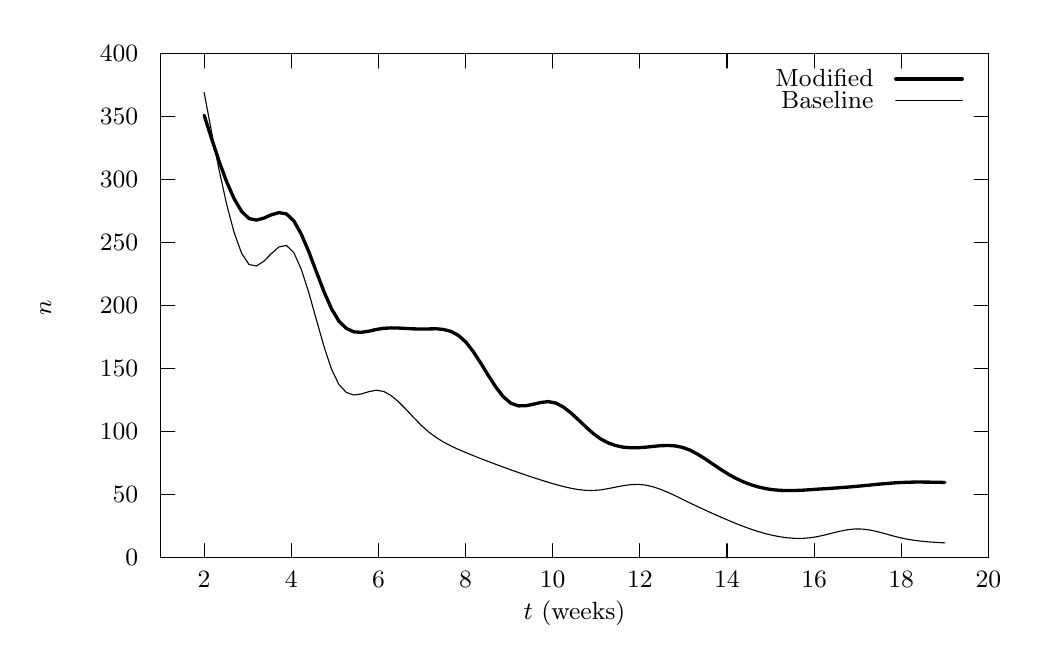
\begin{tikzpicture}[gnuplot]
%% generated with GNUPLOT 4.6p4 (Lua 5.1; terminal rev. 99, script rev. 100)
%% Sun 31 Aug 2014 10:54:04 WST
\tikzset{every node/.append style={font={\fontsize{9pt}{10.8pt}\selectfont}}}
\gpmonochromelines
\path (0.000,0.000) rectangle (12.700,7.620);
\gpcolor{color=gp lt color border}
\gpsetlinetype{gp lt border}
\gpsetlinewidth{1.00}
\draw[gp path] (1.688,0.886)--(1.868,0.886);
\draw[gp path] (12.201,0.886)--(12.021,0.886);
\node[gp node right] at (1.522,0.886) { 0};
\draw[gp path] (1.688,1.686)--(1.868,1.686);
\draw[gp path] (12.201,1.686)--(12.021,1.686);
\node[gp node right] at (1.522,1.686) { 50};
\draw[gp path] (1.688,2.486)--(1.868,2.486);
\draw[gp path] (12.201,2.486)--(12.021,2.486);
\node[gp node right] at (1.522,2.486) { 100};
\draw[gp path] (1.688,3.286)--(1.868,3.286);
\draw[gp path] (12.201,3.286)--(12.021,3.286);
\node[gp node right] at (1.522,3.286) { 150};
\draw[gp path] (1.688,4.087)--(1.868,4.087);
\draw[gp path] (12.201,4.087)--(12.021,4.087);
\node[gp node right] at (1.522,4.087) { 200};
\draw[gp path] (1.688,4.887)--(1.868,4.887);
\draw[gp path] (12.201,4.887)--(12.021,4.887);
\node[gp node right] at (1.522,4.887) { 250};
\draw[gp path] (1.688,5.687)--(1.868,5.687);
\draw[gp path] (12.201,5.687)--(12.021,5.687);
\node[gp node right] at (1.522,5.687) { 300};
\draw[gp path] (1.688,6.487)--(1.868,6.487);
\draw[gp path] (12.201,6.487)--(12.021,6.487);
\node[gp node right] at (1.522,6.487) { 350};
\draw[gp path] (1.688,7.287)--(1.868,7.287);
\draw[gp path] (12.201,7.287)--(12.021,7.287);
\node[gp node right] at (1.522,7.287) { 400};
\draw[gp path] (2.241,0.886)--(2.241,1.066);
\draw[gp path] (2.241,7.287)--(2.241,7.107);
\node[gp node center] at (2.241,0.609) { 2};
\draw[gp path] (3.348,0.886)--(3.348,1.066);
\draw[gp path] (3.348,7.287)--(3.348,7.107);
\node[gp node center] at (3.348,0.609) { 4};
\draw[gp path] (4.455,0.886)--(4.455,1.066);
\draw[gp path] (4.455,7.287)--(4.455,7.107);
\node[gp node center] at (4.455,0.609) { 6};
\draw[gp path] (5.561,0.886)--(5.561,1.066);
\draw[gp path] (5.561,7.287)--(5.561,7.107);
\node[gp node center] at (5.561,0.609) { 8};
\draw[gp path] (6.668,0.886)--(6.668,1.066);
\draw[gp path] (6.668,7.287)--(6.668,7.107);
\node[gp node center] at (6.668,0.609) { 10};
\draw[gp path] (7.774,0.886)--(7.774,1.066);
\draw[gp path] (7.774,7.287)--(7.774,7.107);
\node[gp node center] at (7.774,0.609) { 12};
\draw[gp path] (8.881,0.886)--(8.881,1.066);
\draw[gp path] (8.881,7.287)--(8.881,7.107);
\node[gp node center] at (8.881,0.609) { 14};
\draw[gp path] (9.988,0.886)--(9.988,1.066);
\draw[gp path] (9.988,7.287)--(9.988,7.107);
\node[gp node center] at (9.988,0.609) { 16};
\draw[gp path] (11.094,0.886)--(11.094,1.066);
\draw[gp path] (11.094,7.287)--(11.094,7.107);
\node[gp node center] at (11.094,0.609) { 18};
\draw[gp path] (12.201,0.886)--(12.201,1.066);
\draw[gp path] (12.201,7.287)--(12.201,7.107);
\node[gp node center] at (12.201,0.609) { 20};
\draw[gp path] (1.688,7.287)--(1.688,0.886)--(12.201,0.886)--(12.201,7.287)--cycle;
\node[gp node center,rotate=-270] at (0.221,4.086) {$n$};
\node[gp node center] at (6.944,0.194) {$t$ (weeks)};
\node[gp node right] at (10.859,6.969) {Modified};
\gpcolor{color=gp lt color 0}
\gpsetlinetype{gp lt plot 0}
\gpsetlinewidth{3.00}
\draw[gp path] (11.025,6.969)--(11.869,6.969);
\draw[gp path] (2.241,6.509)--(2.336,6.209)--(2.431,5.923)--(2.526,5.665)--(2.621,5.449)%
  --(2.716,5.288)--(2.811,5.196)--(2.906,5.176)--(3.001,5.202)--(3.096,5.244)--(3.191,5.271)%
  --(3.286,5.255)--(3.381,5.165)--(3.476,4.995)--(3.572,4.770)--(3.667,4.519)--(3.762,4.270)%
  --(3.857,4.053)--(3.952,3.894)--(4.047,3.800)--(4.142,3.757)--(4.237,3.751)--(4.332,3.765)%
  --(4.427,3.787)--(4.522,3.802)--(4.617,3.807)--(4.712,3.805)--(4.807,3.800)--(4.902,3.795)%
  --(4.997,3.792)--(5.092,3.794)--(5.187,3.796)--(5.282,3.787)--(5.377,3.762)--(5.472,3.711)%
  --(5.567,3.625)--(5.662,3.502)--(5.757,3.355)--(5.852,3.200)--(5.947,3.053)--(6.042,2.931)%
  --(6.137,2.850)--(6.232,2.817)--(6.327,2.818)--(6.422,2.838)--(6.517,2.860)--(6.612,2.871)%
  --(6.707,2.853)--(6.802,2.803)--(6.897,2.729)--(6.992,2.642)--(7.087,2.551)--(7.182,2.466)%
  --(7.277,2.397)--(7.372,2.347)--(7.467,2.313)--(7.562,2.293)--(7.657,2.285)--(7.752,2.285)%
  --(7.847,2.292)--(7.942,2.302)--(8.037,2.311)--(8.132,2.314)--(8.227,2.308)--(8.322,2.288)%
  --(8.417,2.252)--(8.512,2.201)--(8.607,2.142)--(8.702,2.077)--(8.797,2.013)--(8.892,1.953)%
  --(8.987,1.900)--(9.082,1.855)--(9.177,1.818)--(9.272,1.789)--(9.367,1.767)--(9.462,1.752)%
  --(9.557,1.744)--(9.652,1.741)--(9.747,1.742)--(9.842,1.746)--(9.937,1.752)--(10.032,1.759)%
  --(10.127,1.765)--(10.222,1.771)--(10.317,1.778)--(10.413,1.785)--(10.508,1.793)--(10.603,1.802)%
  --(10.698,1.811)--(10.793,1.821)--(10.888,1.829)--(10.983,1.837)--(11.078,1.843)--(11.173,1.847)%
  --(11.268,1.849)--(11.363,1.849)--(11.458,1.848)--(11.553,1.847)--(11.648,1.844);
\gpcolor{color=gp lt color border}
\node[gp node right] at (10.859,6.692) {Baseline};
\gpcolor{color=gp lt color 3}
\gpsetlinetype{gp lt plot 3}
\gpsetlinewidth{1.00}
\draw[gp path] (11.025,6.692)--(11.869,6.692);
\draw[gp path] (2.241,6.797)--(2.336,6.293)--(2.431,5.813)--(2.526,5.381)--(2.621,5.021)%
  --(2.716,4.757)--(2.811,4.612)--(2.906,4.593)--(3.001,4.655)--(3.096,4.752)--(3.191,4.835)%
  --(3.286,4.854)--(3.381,4.762)--(3.476,4.548)--(3.572,4.249)--(3.667,3.910)--(3.762,3.575)%
  --(3.857,3.287)--(3.952,3.089)--(4.047,2.987)--(4.142,2.955)--(4.237,2.968)--(4.332,2.997)%
  --(4.427,3.016)--(4.522,3.000)--(4.617,2.947)--(4.712,2.867)--(4.807,2.771)--(4.902,2.669)%
  --(4.997,2.571)--(5.092,2.486)--(5.187,2.416)--(5.282,2.357)--(5.377,2.307)--(5.472,2.263)%
  --(5.567,2.223)--(5.662,2.184)--(5.757,2.146)--(5.852,2.110)--(5.947,2.074)--(6.042,2.039)%
  --(6.137,2.004)--(6.232,1.971)--(6.327,1.938)--(6.422,1.906)--(6.517,1.876)--(6.612,1.846)%
  --(6.707,1.818)--(6.802,1.793)--(6.897,1.771)--(6.992,1.754)--(7.087,1.744)--(7.182,1.742)%
  --(7.277,1.750)--(7.372,1.766)--(7.467,1.785)--(7.562,1.803)--(7.657,1.816)--(7.752,1.820)%
  --(7.847,1.811)--(7.942,1.789)--(8.037,1.757)--(8.132,1.718)--(8.227,1.674)--(8.322,1.627)%
  --(8.417,1.581)--(8.512,1.536)--(8.607,1.492)--(8.702,1.449)--(8.797,1.407)--(8.892,1.366)%
  --(8.987,1.326)--(9.082,1.289)--(9.177,1.254)--(9.272,1.223)--(9.367,1.195)--(9.462,1.172)%
  --(9.557,1.154)--(9.652,1.141)--(9.747,1.134)--(9.842,1.134)--(9.937,1.142)--(10.032,1.157)%
  --(10.127,1.178)--(10.222,1.202)--(10.317,1.225)--(10.413,1.244)--(10.508,1.254)--(10.603,1.252)%
  --(10.698,1.240)--(10.793,1.219)--(10.888,1.194)--(10.983,1.167)--(11.078,1.143)--(11.173,1.123)%
  --(11.268,1.108)--(11.363,1.097)--(11.458,1.088)--(11.553,1.082)--(11.648,1.077);
\gpcolor{color=gp lt color border}
\gpsetlinetype{gp lt border}
\draw[gp path] (1.688,7.287)--(1.688,0.886)--(12.201,0.886)--(12.201,7.287)--cycle;
%% coordinates of the plot area
\gpdefrectangularnode{gp plot 1}{\pgfpoint{1.688cm}{0.886cm}}{\pgfpoint{12.201cm}{7.287cm}}
\end{tikzpicture}
%% gnuplot variables

  \caption{Estimate of number of unfixed defects still in software; comparison}
  \label{comp:remainingbugs}
\end{figure}

\subsection{Testers to Repairing}
We can see from data displayed in figures \ref{comp:dfdf}--\ref{comp:remainingbugs} that moving testers to repair roles has various effects for the different metrics. The primary scenario that represents this move is Scenario D, which moves testers to repairs in the last four weeks.

We see no difference in the ratio of defects found to defects fixed (figure \ref{comp:dfdf}, page \pageref{comp:dfdf}), as by that point in time, most defects have been located and handled. Similarly with the average queue time of major defects (figure \ref{comp:queuetime}, page \pageref{comp:queuetime}). We see a slight difference in the total importance of found defects (figure \ref{comp:tifd}, page \pageref{comp:tifd}) as compared to Scenario B in the final weeks, most likely due to a slightly faster repair cycle. We also see a spike in the estimate of number of unfixed defects (figure \ref{comp:remainingbugs}, page \pageref{comp:remainingbugs}) at the same point where testers move to repairs; this is most likely due to a reevaluation of the exponential regression that is less favourable.

\subsection{Repairers to Testing}
We can see from data displayed in figures \ref{comp:dfdf}--\ref{comp:remainingbugs} that moving repairers to testing roles also has various effects for the different metrics. The primary scenario that represents this move is Scenario B, which moves repairers to testing for the first four weeks.

We see very poor performance in the ratio of defects found to defects fixed due to finding more defects much faster with this allocation of testers. We similarly see poor performance in the total importance of found defects and the average queue time due to this. However, there is a noticeably better performance in the estimate of number of unfixed defects, as the rate of finding defects leads to a regression curve that predicts a much faster downward slope.

\subsection{Optimum Staff Allocation}
To minimise the time major defects went unfound and unfixed, these graphs indicate a dynamic allocation of staff would be in order. An optimum allocation of staff would most likely consist of staff moving between ''sprints`` of finding defects, then fixing them. These sprints would need to be dynamically calculated based on the estimated number of unfound major defects and the amount of staff hours required to fix the current backlog of major defects. There would be an optimisation of many staff being allocated to ''finding`` enough defects that $n$ staff can fix them in exactly $t$ weeks, then those staff moving to repairs to resolve those defects.

This however would most likely lead to highly variable metrics in many cases, so it would be important to choose the correct metrics to ensure customer satisfaction with this approach.

\section{Conclusion}
In conclusion, we can see that while most strategies investigated in this document lead to most, if not all, found defects being resolved before the 20 week test and repair period had elapsed, there was a clear variety in how those strategies showed in the different metrics chosen to be investigated in this report. 

While metrics are objective measures of something, they are not necessary objective measures of the ''heath`` of a software project. Metrics, it has been shown, can be manipulated by different strategies to make them more or less favourable to the customer and to system reliability. Interestingly, this manipulation in most cases has little impact on most defects being resolved before the project's test and repair deadline, but rather the order in which they are resolved.

From a software developer standpoint, clearly the metrics used should inform the testing strategy used, or vice-verse, as customer satisfaction will be tied heavily to those metrics indicating a ''healthy`` software engineering project.

From a customer standpoint, to actually measure the health of the project, it would be naive to choose merely one metric, as it would not provide the requisite data definition to get a true handle on the heath of the software project. It would be important to consider that there are many healthy project scenarios that do not necessarily have metrics that constantly trend downwards and to use a mixture of metrics alongside other qualitative and quantitative data.

%\nocite{*}
%\bibliography{references}

\clearpage
\begin{appendices}
  \section{Results}
Note: Different graphs are not of comparative scale.

  \subsection{Ratio of defects fixed to defects found}
  
  \begin{figure}[!htb]
    \centering
    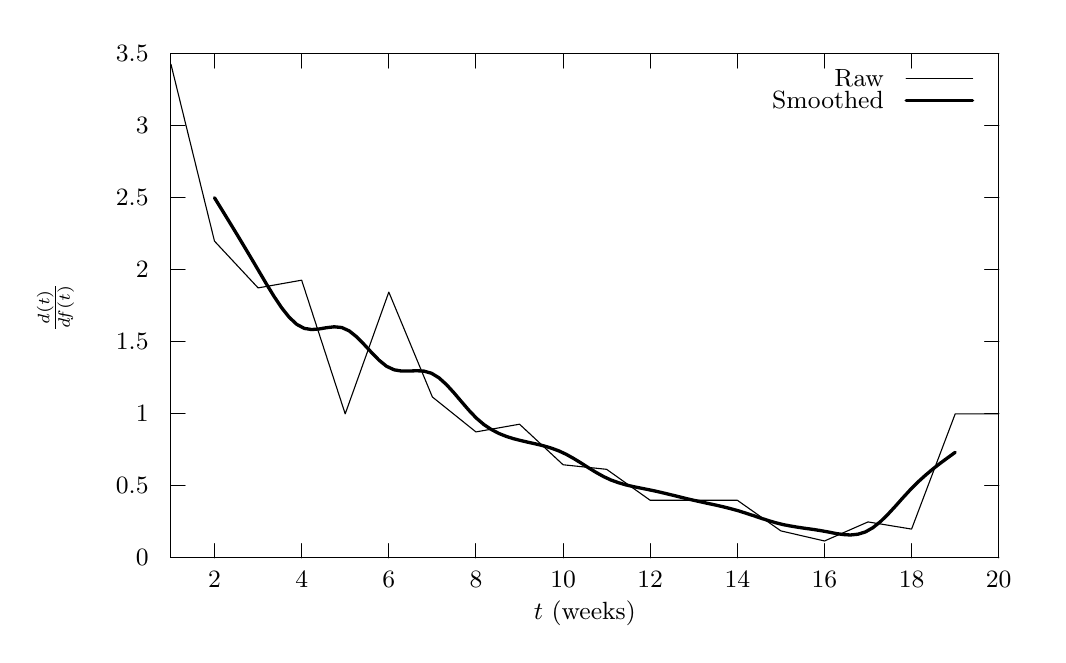
\begin{tikzpicture}[gnuplot]
%% generated with GNUPLOT 4.6p5 (Lua 5.2; terminal rev. 99, script rev. 100)
%% 2/09/2014 2:44:41 PM
\tikzset{every node/.append style={font={\fontsize{9pt}{10.8pt}\selectfont}}}
\gpmonochromelines
\path (0.000,0.000) rectangle (12.700,7.620);
\gpcolor{color=gp lt color border}
\gpsetlinetype{gp lt border}
\gpsetlinewidth{1.00}
\draw[gp path] (1.688,0.886)--(1.868,0.886);
\draw[gp path] (12.201,0.886)--(12.021,0.886);
\node[gp node right] at (1.522,0.886) { 0};
\draw[gp path] (1.688,1.800)--(1.868,1.800);
\draw[gp path] (12.201,1.800)--(12.021,1.800);
\node[gp node right] at (1.522,1.800) { 0.5};
\draw[gp path] (1.688,2.715)--(1.868,2.715);
\draw[gp path] (12.201,2.715)--(12.021,2.715);
\node[gp node right] at (1.522,2.715) { 1};
\draw[gp path] (1.688,3.629)--(1.868,3.629);
\draw[gp path] (12.201,3.629)--(12.021,3.629);
\node[gp node right] at (1.522,3.629) { 1.5};
\draw[gp path] (1.688,4.544)--(1.868,4.544);
\draw[gp path] (12.201,4.544)--(12.021,4.544);
\node[gp node right] at (1.522,4.544) { 2};
\draw[gp path] (1.688,5.458)--(1.868,5.458);
\draw[gp path] (12.201,5.458)--(12.021,5.458);
\node[gp node right] at (1.522,5.458) { 2.5};
\draw[gp path] (1.688,6.373)--(1.868,6.373);
\draw[gp path] (12.201,6.373)--(12.021,6.373);
\node[gp node right] at (1.522,6.373) { 3};
\draw[gp path] (1.688,7.287)--(1.868,7.287);
\draw[gp path] (12.201,7.287)--(12.021,7.287);
\node[gp node right] at (1.522,7.287) { 3.5};
\draw[gp path] (2.241,0.886)--(2.241,1.066);
\draw[gp path] (2.241,7.287)--(2.241,7.107);
\node[gp node center] at (2.241,0.609) { 2};
\draw[gp path] (3.348,0.886)--(3.348,1.066);
\draw[gp path] (3.348,7.287)--(3.348,7.107);
\node[gp node center] at (3.348,0.609) { 4};
\draw[gp path] (4.455,0.886)--(4.455,1.066);
\draw[gp path] (4.455,7.287)--(4.455,7.107);
\node[gp node center] at (4.455,0.609) { 6};
\draw[gp path] (5.561,0.886)--(5.561,1.066);
\draw[gp path] (5.561,7.287)--(5.561,7.107);
\node[gp node center] at (5.561,0.609) { 8};
\draw[gp path] (6.668,0.886)--(6.668,1.066);
\draw[gp path] (6.668,7.287)--(6.668,7.107);
\node[gp node center] at (6.668,0.609) { 10};
\draw[gp path] (7.774,0.886)--(7.774,1.066);
\draw[gp path] (7.774,7.287)--(7.774,7.107);
\node[gp node center] at (7.774,0.609) { 12};
\draw[gp path] (8.881,0.886)--(8.881,1.066);
\draw[gp path] (8.881,7.287)--(8.881,7.107);
\node[gp node center] at (8.881,0.609) { 14};
\draw[gp path] (9.988,0.886)--(9.988,1.066);
\draw[gp path] (9.988,7.287)--(9.988,7.107);
\node[gp node center] at (9.988,0.609) { 16};
\draw[gp path] (11.094,0.886)--(11.094,1.066);
\draw[gp path] (11.094,7.287)--(11.094,7.107);
\node[gp node center] at (11.094,0.609) { 18};
\draw[gp path] (12.201,0.886)--(12.201,1.066);
\draw[gp path] (12.201,7.287)--(12.201,7.107);
\node[gp node center] at (12.201,0.609) { 20};
\draw[gp path] (1.688,7.287)--(1.688,0.886)--(12.201,0.886)--(12.201,7.287)--cycle;
\node[gp node center,rotate=-270] at (0.221,4.086) {$\frac{d(t)}{df(t)}$};
\node[gp node center] at (6.944,0.194) {$t$ (weeks)};
\node[gp node right] at (10.859,6.969) {Raw};
\gpcolor{color=gp lt color 3}
\gpsetlinetype{gp lt plot 3}
\draw[gp path] (11.025,6.969)--(11.869,6.969);
\draw[gp path] (1.688,7.156)--(2.241,4.909)--(2.795,4.315)--(3.348,4.413)--(3.901,2.715)%
  --(4.455,4.262)--(5.008,2.930)--(5.561,2.486)--(6.115,2.584)--(6.668,2.069)--(7.221,2.011)%
  --(7.774,1.618)--(8.328,1.618)--(8.881,1.618)--(9.434,1.229)--(9.988,1.101)--(10.541,1.343)%
  --(11.094,1.252)--(11.648,2.715)--(12.201,2.715);
\gpcolor{color=gp lt color border}
\node[gp node right] at (10.859,6.692) {Smoothed};
\gpcolor{color=gp lt color 0}
\gpsetlinetype{gp lt plot 0}
\gpsetlinewidth{3.00}
\draw[gp path] (11.025,6.692)--(11.869,6.692);
\draw[gp path] (2.241,5.460)--(2.336,5.306)--(2.431,5.151)--(2.526,4.995)--(2.621,4.837)%
  --(2.716,4.678)--(2.811,4.517)--(2.906,4.356)--(3.001,4.201)--(3.096,4.060)--(3.191,3.941)%
  --(3.286,3.852)--(3.381,3.801)--(3.476,3.786)--(3.572,3.794)--(3.667,3.810)--(3.762,3.821)%
  --(3.857,3.812)--(3.952,3.769)--(4.047,3.693)--(4.142,3.596)--(4.237,3.493)--(4.332,3.396)%
  --(4.427,3.319)--(4.522,3.275)--(4.617,3.259)--(4.712,3.259)--(4.807,3.263)--(4.902,3.258)%
  --(4.997,3.231)--(5.092,3.173)--(5.187,3.087)--(5.282,2.983)--(5.377,2.871)--(5.472,2.761)%
  --(5.567,2.661)--(5.662,2.580)--(5.757,2.517)--(5.852,2.467)--(5.947,2.429)--(6.042,2.399)%
  --(6.137,2.375)--(6.232,2.353)--(6.327,2.332)--(6.422,2.309)--(6.517,2.281)--(6.612,2.246)%
  --(6.707,2.202)--(6.802,2.149)--(6.897,2.091)--(6.992,2.030)--(7.087,1.972)--(7.182,1.919)%
  --(7.277,1.875)--(7.372,1.841)--(7.467,1.813)--(7.562,1.791)--(7.657,1.772)--(7.752,1.753)%
  --(7.847,1.733)--(7.942,1.711)--(8.037,1.688)--(8.132,1.665)--(8.227,1.641)--(8.322,1.619)%
  --(8.417,1.598)--(8.512,1.577)--(8.607,1.557)--(8.702,1.535)--(8.797,1.511)--(8.892,1.485)%
  --(8.987,1.455)--(9.082,1.424)--(9.177,1.392)--(9.272,1.361)--(9.367,1.333)--(9.462,1.309)%
  --(9.557,1.291)--(9.652,1.275)--(9.747,1.261)--(9.842,1.248)--(9.937,1.233)--(10.032,1.216)%
  --(10.127,1.197)--(10.222,1.183)--(10.317,1.177)--(10.413,1.187)--(10.508,1.216)--(10.603,1.270)%
  --(10.698,1.346)--(10.793,1.439)--(10.888,1.542)--(10.983,1.649)--(11.078,1.752)--(11.173,1.848)%
  --(11.268,1.934)--(11.363,2.014)--(11.458,2.088)--(11.553,2.158)--(11.648,2.227);
\gpcolor{color=gp lt color border}
\gpsetlinetype{gp lt border}
\gpsetlinewidth{1.00}
\draw[gp path] (1.688,7.287)--(1.688,0.886)--(12.201,0.886)--(12.201,7.287)--cycle;
%% coordinates of the plot area
\gpdefrectangularnode{gp plot 1}{\pgfpoint{1.688cm}{0.886cm}}{\pgfpoint{12.201cm}{7.287cm}}
\end{tikzpicture}
%% gnuplot variables

    \caption{Easy--Hard, Major--Minor}
  \end{figure}
  
  \begin{figure}[!htb]
    \centering
    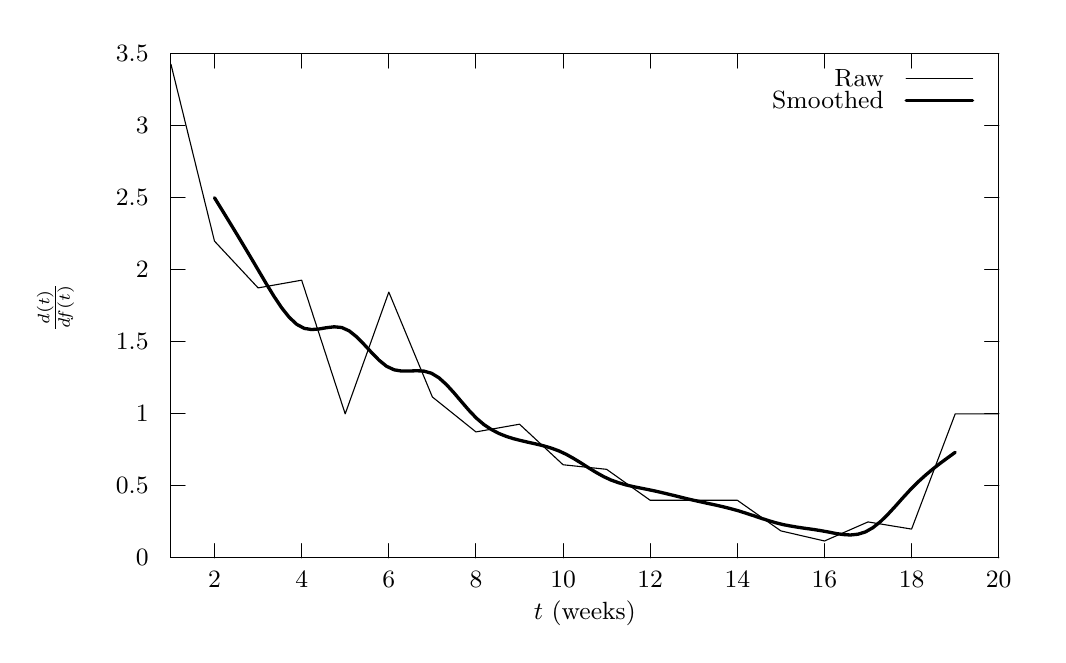
\begin{tikzpicture}[gnuplot]
%% generated with GNUPLOT 4.6p5 (Lua 5.2; terminal rev. 99, script rev. 100)
%% 2/09/2014 2:44:41 PM
\tikzset{every node/.append style={font={\fontsize{9pt}{10.8pt}\selectfont}}}
\gpmonochromelines
\path (0.000,0.000) rectangle (12.700,7.620);
\gpcolor{color=gp lt color border}
\gpsetlinetype{gp lt border}
\gpsetlinewidth{1.00}
\draw[gp path] (1.688,0.886)--(1.868,0.886);
\draw[gp path] (12.201,0.886)--(12.021,0.886);
\node[gp node right] at (1.522,0.886) { 0};
\draw[gp path] (1.688,1.800)--(1.868,1.800);
\draw[gp path] (12.201,1.800)--(12.021,1.800);
\node[gp node right] at (1.522,1.800) { 0.5};
\draw[gp path] (1.688,2.715)--(1.868,2.715);
\draw[gp path] (12.201,2.715)--(12.021,2.715);
\node[gp node right] at (1.522,2.715) { 1};
\draw[gp path] (1.688,3.629)--(1.868,3.629);
\draw[gp path] (12.201,3.629)--(12.021,3.629);
\node[gp node right] at (1.522,3.629) { 1.5};
\draw[gp path] (1.688,4.544)--(1.868,4.544);
\draw[gp path] (12.201,4.544)--(12.021,4.544);
\node[gp node right] at (1.522,4.544) { 2};
\draw[gp path] (1.688,5.458)--(1.868,5.458);
\draw[gp path] (12.201,5.458)--(12.021,5.458);
\node[gp node right] at (1.522,5.458) { 2.5};
\draw[gp path] (1.688,6.373)--(1.868,6.373);
\draw[gp path] (12.201,6.373)--(12.021,6.373);
\node[gp node right] at (1.522,6.373) { 3};
\draw[gp path] (1.688,7.287)--(1.868,7.287);
\draw[gp path] (12.201,7.287)--(12.021,7.287);
\node[gp node right] at (1.522,7.287) { 3.5};
\draw[gp path] (2.241,0.886)--(2.241,1.066);
\draw[gp path] (2.241,7.287)--(2.241,7.107);
\node[gp node center] at (2.241,0.609) { 2};
\draw[gp path] (3.348,0.886)--(3.348,1.066);
\draw[gp path] (3.348,7.287)--(3.348,7.107);
\node[gp node center] at (3.348,0.609) { 4};
\draw[gp path] (4.455,0.886)--(4.455,1.066);
\draw[gp path] (4.455,7.287)--(4.455,7.107);
\node[gp node center] at (4.455,0.609) { 6};
\draw[gp path] (5.561,0.886)--(5.561,1.066);
\draw[gp path] (5.561,7.287)--(5.561,7.107);
\node[gp node center] at (5.561,0.609) { 8};
\draw[gp path] (6.668,0.886)--(6.668,1.066);
\draw[gp path] (6.668,7.287)--(6.668,7.107);
\node[gp node center] at (6.668,0.609) { 10};
\draw[gp path] (7.774,0.886)--(7.774,1.066);
\draw[gp path] (7.774,7.287)--(7.774,7.107);
\node[gp node center] at (7.774,0.609) { 12};
\draw[gp path] (8.881,0.886)--(8.881,1.066);
\draw[gp path] (8.881,7.287)--(8.881,7.107);
\node[gp node center] at (8.881,0.609) { 14};
\draw[gp path] (9.988,0.886)--(9.988,1.066);
\draw[gp path] (9.988,7.287)--(9.988,7.107);
\node[gp node center] at (9.988,0.609) { 16};
\draw[gp path] (11.094,0.886)--(11.094,1.066);
\draw[gp path] (11.094,7.287)--(11.094,7.107);
\node[gp node center] at (11.094,0.609) { 18};
\draw[gp path] (12.201,0.886)--(12.201,1.066);
\draw[gp path] (12.201,7.287)--(12.201,7.107);
\node[gp node center] at (12.201,0.609) { 20};
\draw[gp path] (1.688,7.287)--(1.688,0.886)--(12.201,0.886)--(12.201,7.287)--cycle;
\node[gp node center,rotate=-270] at (0.221,4.086) {$\frac{d(t)}{df(t)}$};
\node[gp node center] at (6.944,0.194) {$t$ (weeks)};
\node[gp node right] at (10.859,6.969) {Raw};
\gpcolor{color=gp lt color 3}
\gpsetlinetype{gp lt plot 3}
\draw[gp path] (11.025,6.969)--(11.869,6.969);
\draw[gp path] (1.688,7.156)--(2.241,4.909)--(2.795,4.315)--(3.348,4.413)--(3.901,2.715)%
  --(4.455,4.262)--(5.008,2.930)--(5.561,2.486)--(6.115,2.584)--(6.668,2.069)--(7.221,2.011)%
  --(7.774,1.618)--(8.328,1.618)--(8.881,1.618)--(9.434,1.229)--(9.988,1.101)--(10.541,1.343)%
  --(11.094,1.252)--(11.648,2.715)--(12.201,2.715);
\gpcolor{color=gp lt color border}
\node[gp node right] at (10.859,6.692) {Smoothed};
\gpcolor{color=gp lt color 0}
\gpsetlinetype{gp lt plot 0}
\gpsetlinewidth{3.00}
\draw[gp path] (11.025,6.692)--(11.869,6.692);
\draw[gp path] (2.241,5.460)--(2.336,5.306)--(2.431,5.151)--(2.526,4.995)--(2.621,4.837)%
  --(2.716,4.678)--(2.811,4.517)--(2.906,4.356)--(3.001,4.201)--(3.096,4.060)--(3.191,3.941)%
  --(3.286,3.852)--(3.381,3.801)--(3.476,3.786)--(3.572,3.794)--(3.667,3.810)--(3.762,3.821)%
  --(3.857,3.812)--(3.952,3.769)--(4.047,3.693)--(4.142,3.596)--(4.237,3.493)--(4.332,3.396)%
  --(4.427,3.319)--(4.522,3.275)--(4.617,3.259)--(4.712,3.259)--(4.807,3.263)--(4.902,3.258)%
  --(4.997,3.231)--(5.092,3.173)--(5.187,3.087)--(5.282,2.983)--(5.377,2.871)--(5.472,2.761)%
  --(5.567,2.661)--(5.662,2.580)--(5.757,2.517)--(5.852,2.467)--(5.947,2.429)--(6.042,2.399)%
  --(6.137,2.375)--(6.232,2.353)--(6.327,2.332)--(6.422,2.309)--(6.517,2.281)--(6.612,2.246)%
  --(6.707,2.202)--(6.802,2.149)--(6.897,2.091)--(6.992,2.030)--(7.087,1.972)--(7.182,1.919)%
  --(7.277,1.875)--(7.372,1.841)--(7.467,1.813)--(7.562,1.791)--(7.657,1.772)--(7.752,1.753)%
  --(7.847,1.733)--(7.942,1.711)--(8.037,1.688)--(8.132,1.665)--(8.227,1.641)--(8.322,1.619)%
  --(8.417,1.598)--(8.512,1.577)--(8.607,1.557)--(8.702,1.535)--(8.797,1.511)--(8.892,1.485)%
  --(8.987,1.455)--(9.082,1.424)--(9.177,1.392)--(9.272,1.361)--(9.367,1.333)--(9.462,1.309)%
  --(9.557,1.291)--(9.652,1.275)--(9.747,1.261)--(9.842,1.248)--(9.937,1.233)--(10.032,1.216)%
  --(10.127,1.197)--(10.222,1.183)--(10.317,1.177)--(10.413,1.187)--(10.508,1.216)--(10.603,1.270)%
  --(10.698,1.346)--(10.793,1.439)--(10.888,1.542)--(10.983,1.649)--(11.078,1.752)--(11.173,1.848)%
  --(11.268,1.934)--(11.363,2.014)--(11.458,2.088)--(11.553,2.158)--(11.648,2.227);
\gpcolor{color=gp lt color border}
\gpsetlinetype{gp lt border}
\gpsetlinewidth{1.00}
\draw[gp path] (1.688,7.287)--(1.688,0.886)--(12.201,0.886)--(12.201,7.287)--cycle;
%% coordinates of the plot area
\gpdefrectangularnode{gp plot 1}{\pgfpoint{1.688cm}{0.886cm}}{\pgfpoint{12.201cm}{7.287cm}}
\end{tikzpicture}
%% gnuplot variables

    \caption{Hard--Easy, Major--Minor}
  \end{figure}
  
  \begin{figure}[!htb]
    \centering
    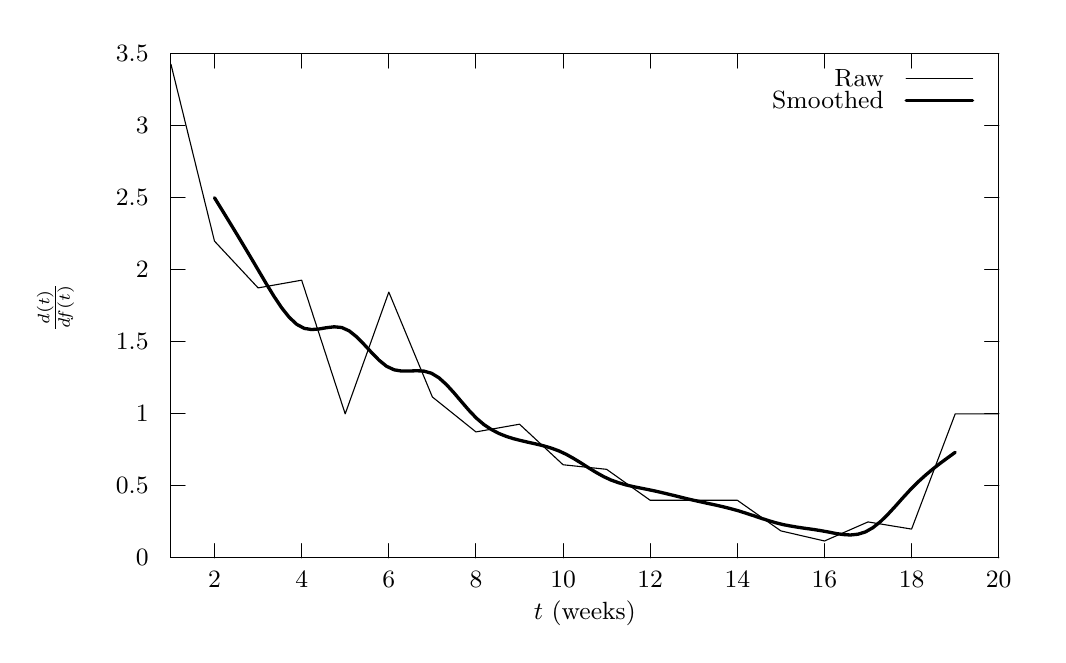
\begin{tikzpicture}[gnuplot]
%% generated with GNUPLOT 4.6p5 (Lua 5.2; terminal rev. 99, script rev. 100)
%% 2/09/2014 2:44:41 PM
\tikzset{every node/.append style={font={\fontsize{9pt}{10.8pt}\selectfont}}}
\gpmonochromelines
\path (0.000,0.000) rectangle (12.700,7.620);
\gpcolor{color=gp lt color border}
\gpsetlinetype{gp lt border}
\gpsetlinewidth{1.00}
\draw[gp path] (1.688,0.886)--(1.868,0.886);
\draw[gp path] (12.201,0.886)--(12.021,0.886);
\node[gp node right] at (1.522,0.886) { 0};
\draw[gp path] (1.688,1.800)--(1.868,1.800);
\draw[gp path] (12.201,1.800)--(12.021,1.800);
\node[gp node right] at (1.522,1.800) { 0.5};
\draw[gp path] (1.688,2.715)--(1.868,2.715);
\draw[gp path] (12.201,2.715)--(12.021,2.715);
\node[gp node right] at (1.522,2.715) { 1};
\draw[gp path] (1.688,3.629)--(1.868,3.629);
\draw[gp path] (12.201,3.629)--(12.021,3.629);
\node[gp node right] at (1.522,3.629) { 1.5};
\draw[gp path] (1.688,4.544)--(1.868,4.544);
\draw[gp path] (12.201,4.544)--(12.021,4.544);
\node[gp node right] at (1.522,4.544) { 2};
\draw[gp path] (1.688,5.458)--(1.868,5.458);
\draw[gp path] (12.201,5.458)--(12.021,5.458);
\node[gp node right] at (1.522,5.458) { 2.5};
\draw[gp path] (1.688,6.373)--(1.868,6.373);
\draw[gp path] (12.201,6.373)--(12.021,6.373);
\node[gp node right] at (1.522,6.373) { 3};
\draw[gp path] (1.688,7.287)--(1.868,7.287);
\draw[gp path] (12.201,7.287)--(12.021,7.287);
\node[gp node right] at (1.522,7.287) { 3.5};
\draw[gp path] (2.241,0.886)--(2.241,1.066);
\draw[gp path] (2.241,7.287)--(2.241,7.107);
\node[gp node center] at (2.241,0.609) { 2};
\draw[gp path] (3.348,0.886)--(3.348,1.066);
\draw[gp path] (3.348,7.287)--(3.348,7.107);
\node[gp node center] at (3.348,0.609) { 4};
\draw[gp path] (4.455,0.886)--(4.455,1.066);
\draw[gp path] (4.455,7.287)--(4.455,7.107);
\node[gp node center] at (4.455,0.609) { 6};
\draw[gp path] (5.561,0.886)--(5.561,1.066);
\draw[gp path] (5.561,7.287)--(5.561,7.107);
\node[gp node center] at (5.561,0.609) { 8};
\draw[gp path] (6.668,0.886)--(6.668,1.066);
\draw[gp path] (6.668,7.287)--(6.668,7.107);
\node[gp node center] at (6.668,0.609) { 10};
\draw[gp path] (7.774,0.886)--(7.774,1.066);
\draw[gp path] (7.774,7.287)--(7.774,7.107);
\node[gp node center] at (7.774,0.609) { 12};
\draw[gp path] (8.881,0.886)--(8.881,1.066);
\draw[gp path] (8.881,7.287)--(8.881,7.107);
\node[gp node center] at (8.881,0.609) { 14};
\draw[gp path] (9.988,0.886)--(9.988,1.066);
\draw[gp path] (9.988,7.287)--(9.988,7.107);
\node[gp node center] at (9.988,0.609) { 16};
\draw[gp path] (11.094,0.886)--(11.094,1.066);
\draw[gp path] (11.094,7.287)--(11.094,7.107);
\node[gp node center] at (11.094,0.609) { 18};
\draw[gp path] (12.201,0.886)--(12.201,1.066);
\draw[gp path] (12.201,7.287)--(12.201,7.107);
\node[gp node center] at (12.201,0.609) { 20};
\draw[gp path] (1.688,7.287)--(1.688,0.886)--(12.201,0.886)--(12.201,7.287)--cycle;
\node[gp node center,rotate=-270] at (0.221,4.086) {$\frac{d(t)}{df(t)}$};
\node[gp node center] at (6.944,0.194) {$t$ (weeks)};
\node[gp node right] at (10.859,6.969) {Raw};
\gpcolor{color=gp lt color 3}
\gpsetlinetype{gp lt plot 3}
\draw[gp path] (11.025,6.969)--(11.869,6.969);
\draw[gp path] (1.688,7.156)--(2.241,4.909)--(2.795,4.315)--(3.348,4.413)--(3.901,2.715)%
  --(4.455,4.262)--(5.008,2.930)--(5.561,2.486)--(6.115,2.584)--(6.668,2.069)--(7.221,2.011)%
  --(7.774,1.618)--(8.328,1.618)--(8.881,1.618)--(9.434,1.229)--(9.988,1.101)--(10.541,1.343)%
  --(11.094,1.252)--(11.648,2.715)--(12.201,2.715);
\gpcolor{color=gp lt color border}
\node[gp node right] at (10.859,6.692) {Smoothed};
\gpcolor{color=gp lt color 0}
\gpsetlinetype{gp lt plot 0}
\gpsetlinewidth{3.00}
\draw[gp path] (11.025,6.692)--(11.869,6.692);
\draw[gp path] (2.241,5.460)--(2.336,5.306)--(2.431,5.151)--(2.526,4.995)--(2.621,4.837)%
  --(2.716,4.678)--(2.811,4.517)--(2.906,4.356)--(3.001,4.201)--(3.096,4.060)--(3.191,3.941)%
  --(3.286,3.852)--(3.381,3.801)--(3.476,3.786)--(3.572,3.794)--(3.667,3.810)--(3.762,3.821)%
  --(3.857,3.812)--(3.952,3.769)--(4.047,3.693)--(4.142,3.596)--(4.237,3.493)--(4.332,3.396)%
  --(4.427,3.319)--(4.522,3.275)--(4.617,3.259)--(4.712,3.259)--(4.807,3.263)--(4.902,3.258)%
  --(4.997,3.231)--(5.092,3.173)--(5.187,3.087)--(5.282,2.983)--(5.377,2.871)--(5.472,2.761)%
  --(5.567,2.661)--(5.662,2.580)--(5.757,2.517)--(5.852,2.467)--(5.947,2.429)--(6.042,2.399)%
  --(6.137,2.375)--(6.232,2.353)--(6.327,2.332)--(6.422,2.309)--(6.517,2.281)--(6.612,2.246)%
  --(6.707,2.202)--(6.802,2.149)--(6.897,2.091)--(6.992,2.030)--(7.087,1.972)--(7.182,1.919)%
  --(7.277,1.875)--(7.372,1.841)--(7.467,1.813)--(7.562,1.791)--(7.657,1.772)--(7.752,1.753)%
  --(7.847,1.733)--(7.942,1.711)--(8.037,1.688)--(8.132,1.665)--(8.227,1.641)--(8.322,1.619)%
  --(8.417,1.598)--(8.512,1.577)--(8.607,1.557)--(8.702,1.535)--(8.797,1.511)--(8.892,1.485)%
  --(8.987,1.455)--(9.082,1.424)--(9.177,1.392)--(9.272,1.361)--(9.367,1.333)--(9.462,1.309)%
  --(9.557,1.291)--(9.652,1.275)--(9.747,1.261)--(9.842,1.248)--(9.937,1.233)--(10.032,1.216)%
  --(10.127,1.197)--(10.222,1.183)--(10.317,1.177)--(10.413,1.187)--(10.508,1.216)--(10.603,1.270)%
  --(10.698,1.346)--(10.793,1.439)--(10.888,1.542)--(10.983,1.649)--(11.078,1.752)--(11.173,1.848)%
  --(11.268,1.934)--(11.363,2.014)--(11.458,2.088)--(11.553,2.158)--(11.648,2.227);
\gpcolor{color=gp lt color border}
\gpsetlinetype{gp lt border}
\gpsetlinewidth{1.00}
\draw[gp path] (1.688,7.287)--(1.688,0.886)--(12.201,0.886)--(12.201,7.287)--cycle;
%% coordinates of the plot area
\gpdefrectangularnode{gp plot 1}{\pgfpoint{1.688cm}{0.886cm}}{\pgfpoint{12.201cm}{7.287cm}}
\end{tikzpicture}
%% gnuplot variables

    \caption{Major--Minor, Easy--Hard}
  \end{figure}
  
  \begin{figure}[!htb]
    \centering
    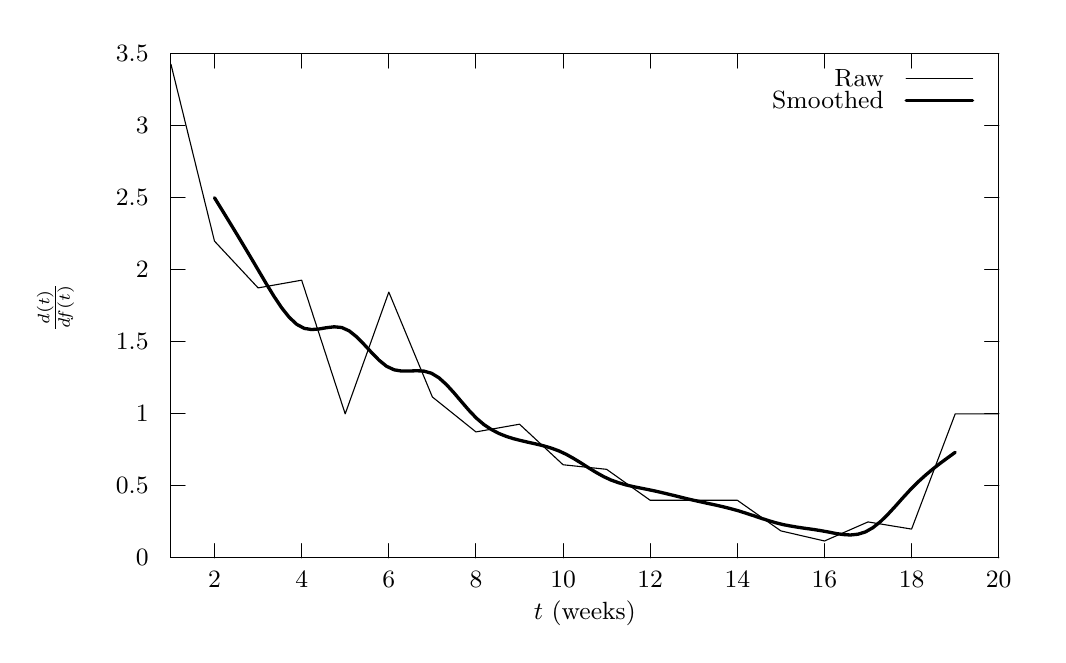
\begin{tikzpicture}[gnuplot]
%% generated with GNUPLOT 4.6p5 (Lua 5.2; terminal rev. 99, script rev. 100)
%% 2/09/2014 2:44:41 PM
\tikzset{every node/.append style={font={\fontsize{9pt}{10.8pt}\selectfont}}}
\gpmonochromelines
\path (0.000,0.000) rectangle (12.700,7.620);
\gpcolor{color=gp lt color border}
\gpsetlinetype{gp lt border}
\gpsetlinewidth{1.00}
\draw[gp path] (1.688,0.886)--(1.868,0.886);
\draw[gp path] (12.201,0.886)--(12.021,0.886);
\node[gp node right] at (1.522,0.886) { 0};
\draw[gp path] (1.688,1.800)--(1.868,1.800);
\draw[gp path] (12.201,1.800)--(12.021,1.800);
\node[gp node right] at (1.522,1.800) { 0.5};
\draw[gp path] (1.688,2.715)--(1.868,2.715);
\draw[gp path] (12.201,2.715)--(12.021,2.715);
\node[gp node right] at (1.522,2.715) { 1};
\draw[gp path] (1.688,3.629)--(1.868,3.629);
\draw[gp path] (12.201,3.629)--(12.021,3.629);
\node[gp node right] at (1.522,3.629) { 1.5};
\draw[gp path] (1.688,4.544)--(1.868,4.544);
\draw[gp path] (12.201,4.544)--(12.021,4.544);
\node[gp node right] at (1.522,4.544) { 2};
\draw[gp path] (1.688,5.458)--(1.868,5.458);
\draw[gp path] (12.201,5.458)--(12.021,5.458);
\node[gp node right] at (1.522,5.458) { 2.5};
\draw[gp path] (1.688,6.373)--(1.868,6.373);
\draw[gp path] (12.201,6.373)--(12.021,6.373);
\node[gp node right] at (1.522,6.373) { 3};
\draw[gp path] (1.688,7.287)--(1.868,7.287);
\draw[gp path] (12.201,7.287)--(12.021,7.287);
\node[gp node right] at (1.522,7.287) { 3.5};
\draw[gp path] (2.241,0.886)--(2.241,1.066);
\draw[gp path] (2.241,7.287)--(2.241,7.107);
\node[gp node center] at (2.241,0.609) { 2};
\draw[gp path] (3.348,0.886)--(3.348,1.066);
\draw[gp path] (3.348,7.287)--(3.348,7.107);
\node[gp node center] at (3.348,0.609) { 4};
\draw[gp path] (4.455,0.886)--(4.455,1.066);
\draw[gp path] (4.455,7.287)--(4.455,7.107);
\node[gp node center] at (4.455,0.609) { 6};
\draw[gp path] (5.561,0.886)--(5.561,1.066);
\draw[gp path] (5.561,7.287)--(5.561,7.107);
\node[gp node center] at (5.561,0.609) { 8};
\draw[gp path] (6.668,0.886)--(6.668,1.066);
\draw[gp path] (6.668,7.287)--(6.668,7.107);
\node[gp node center] at (6.668,0.609) { 10};
\draw[gp path] (7.774,0.886)--(7.774,1.066);
\draw[gp path] (7.774,7.287)--(7.774,7.107);
\node[gp node center] at (7.774,0.609) { 12};
\draw[gp path] (8.881,0.886)--(8.881,1.066);
\draw[gp path] (8.881,7.287)--(8.881,7.107);
\node[gp node center] at (8.881,0.609) { 14};
\draw[gp path] (9.988,0.886)--(9.988,1.066);
\draw[gp path] (9.988,7.287)--(9.988,7.107);
\node[gp node center] at (9.988,0.609) { 16};
\draw[gp path] (11.094,0.886)--(11.094,1.066);
\draw[gp path] (11.094,7.287)--(11.094,7.107);
\node[gp node center] at (11.094,0.609) { 18};
\draw[gp path] (12.201,0.886)--(12.201,1.066);
\draw[gp path] (12.201,7.287)--(12.201,7.107);
\node[gp node center] at (12.201,0.609) { 20};
\draw[gp path] (1.688,7.287)--(1.688,0.886)--(12.201,0.886)--(12.201,7.287)--cycle;
\node[gp node center,rotate=-270] at (0.221,4.086) {$\frac{d(t)}{df(t)}$};
\node[gp node center] at (6.944,0.194) {$t$ (weeks)};
\node[gp node right] at (10.859,6.969) {Raw};
\gpcolor{color=gp lt color 3}
\gpsetlinetype{gp lt plot 3}
\draw[gp path] (11.025,6.969)--(11.869,6.969);
\draw[gp path] (1.688,7.156)--(2.241,4.909)--(2.795,4.315)--(3.348,4.413)--(3.901,2.715)%
  --(4.455,4.262)--(5.008,2.930)--(5.561,2.486)--(6.115,2.584)--(6.668,2.069)--(7.221,2.011)%
  --(7.774,1.618)--(8.328,1.618)--(8.881,1.618)--(9.434,1.229)--(9.988,1.101)--(10.541,1.343)%
  --(11.094,1.252)--(11.648,2.715)--(12.201,2.715);
\gpcolor{color=gp lt color border}
\node[gp node right] at (10.859,6.692) {Smoothed};
\gpcolor{color=gp lt color 0}
\gpsetlinetype{gp lt plot 0}
\gpsetlinewidth{3.00}
\draw[gp path] (11.025,6.692)--(11.869,6.692);
\draw[gp path] (2.241,5.460)--(2.336,5.306)--(2.431,5.151)--(2.526,4.995)--(2.621,4.837)%
  --(2.716,4.678)--(2.811,4.517)--(2.906,4.356)--(3.001,4.201)--(3.096,4.060)--(3.191,3.941)%
  --(3.286,3.852)--(3.381,3.801)--(3.476,3.786)--(3.572,3.794)--(3.667,3.810)--(3.762,3.821)%
  --(3.857,3.812)--(3.952,3.769)--(4.047,3.693)--(4.142,3.596)--(4.237,3.493)--(4.332,3.396)%
  --(4.427,3.319)--(4.522,3.275)--(4.617,3.259)--(4.712,3.259)--(4.807,3.263)--(4.902,3.258)%
  --(4.997,3.231)--(5.092,3.173)--(5.187,3.087)--(5.282,2.983)--(5.377,2.871)--(5.472,2.761)%
  --(5.567,2.661)--(5.662,2.580)--(5.757,2.517)--(5.852,2.467)--(5.947,2.429)--(6.042,2.399)%
  --(6.137,2.375)--(6.232,2.353)--(6.327,2.332)--(6.422,2.309)--(6.517,2.281)--(6.612,2.246)%
  --(6.707,2.202)--(6.802,2.149)--(6.897,2.091)--(6.992,2.030)--(7.087,1.972)--(7.182,1.919)%
  --(7.277,1.875)--(7.372,1.841)--(7.467,1.813)--(7.562,1.791)--(7.657,1.772)--(7.752,1.753)%
  --(7.847,1.733)--(7.942,1.711)--(8.037,1.688)--(8.132,1.665)--(8.227,1.641)--(8.322,1.619)%
  --(8.417,1.598)--(8.512,1.577)--(8.607,1.557)--(8.702,1.535)--(8.797,1.511)--(8.892,1.485)%
  --(8.987,1.455)--(9.082,1.424)--(9.177,1.392)--(9.272,1.361)--(9.367,1.333)--(9.462,1.309)%
  --(9.557,1.291)--(9.652,1.275)--(9.747,1.261)--(9.842,1.248)--(9.937,1.233)--(10.032,1.216)%
  --(10.127,1.197)--(10.222,1.183)--(10.317,1.177)--(10.413,1.187)--(10.508,1.216)--(10.603,1.270)%
  --(10.698,1.346)--(10.793,1.439)--(10.888,1.542)--(10.983,1.649)--(11.078,1.752)--(11.173,1.848)%
  --(11.268,1.934)--(11.363,2.014)--(11.458,2.088)--(11.553,2.158)--(11.648,2.227);
\gpcolor{color=gp lt color border}
\gpsetlinetype{gp lt border}
\gpsetlinewidth{1.00}
\draw[gp path] (1.688,7.287)--(1.688,0.886)--(12.201,0.886)--(12.201,7.287)--cycle;
%% coordinates of the plot area
\gpdefrectangularnode{gp plot 1}{\pgfpoint{1.688cm}{0.886cm}}{\pgfpoint{12.201cm}{7.287cm}}
\end{tikzpicture}
%% gnuplot variables

    \caption{Minor--Major, Easy--Hard}
  \end{figure}
  
  \begin{figure}[!htb]
    \centering
    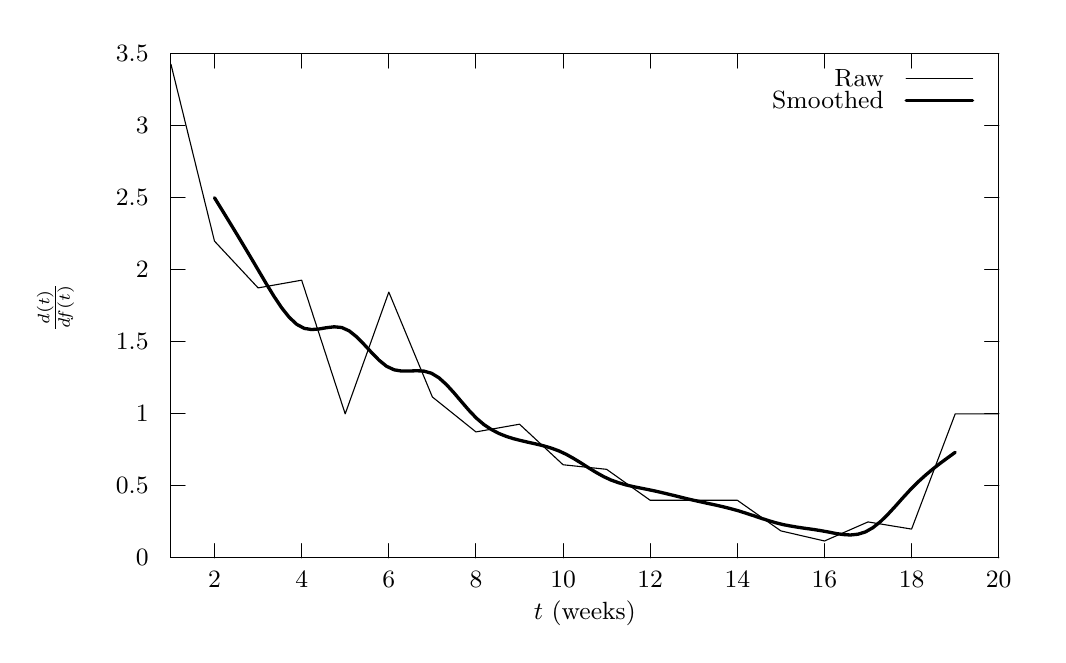
\begin{tikzpicture}[gnuplot]
%% generated with GNUPLOT 4.6p5 (Lua 5.2; terminal rev. 99, script rev. 100)
%% 2/09/2014 2:44:41 PM
\tikzset{every node/.append style={font={\fontsize{9pt}{10.8pt}\selectfont}}}
\gpmonochromelines
\path (0.000,0.000) rectangle (12.700,7.620);
\gpcolor{color=gp lt color border}
\gpsetlinetype{gp lt border}
\gpsetlinewidth{1.00}
\draw[gp path] (1.688,0.886)--(1.868,0.886);
\draw[gp path] (12.201,0.886)--(12.021,0.886);
\node[gp node right] at (1.522,0.886) { 0};
\draw[gp path] (1.688,1.800)--(1.868,1.800);
\draw[gp path] (12.201,1.800)--(12.021,1.800);
\node[gp node right] at (1.522,1.800) { 0.5};
\draw[gp path] (1.688,2.715)--(1.868,2.715);
\draw[gp path] (12.201,2.715)--(12.021,2.715);
\node[gp node right] at (1.522,2.715) { 1};
\draw[gp path] (1.688,3.629)--(1.868,3.629);
\draw[gp path] (12.201,3.629)--(12.021,3.629);
\node[gp node right] at (1.522,3.629) { 1.5};
\draw[gp path] (1.688,4.544)--(1.868,4.544);
\draw[gp path] (12.201,4.544)--(12.021,4.544);
\node[gp node right] at (1.522,4.544) { 2};
\draw[gp path] (1.688,5.458)--(1.868,5.458);
\draw[gp path] (12.201,5.458)--(12.021,5.458);
\node[gp node right] at (1.522,5.458) { 2.5};
\draw[gp path] (1.688,6.373)--(1.868,6.373);
\draw[gp path] (12.201,6.373)--(12.021,6.373);
\node[gp node right] at (1.522,6.373) { 3};
\draw[gp path] (1.688,7.287)--(1.868,7.287);
\draw[gp path] (12.201,7.287)--(12.021,7.287);
\node[gp node right] at (1.522,7.287) { 3.5};
\draw[gp path] (2.241,0.886)--(2.241,1.066);
\draw[gp path] (2.241,7.287)--(2.241,7.107);
\node[gp node center] at (2.241,0.609) { 2};
\draw[gp path] (3.348,0.886)--(3.348,1.066);
\draw[gp path] (3.348,7.287)--(3.348,7.107);
\node[gp node center] at (3.348,0.609) { 4};
\draw[gp path] (4.455,0.886)--(4.455,1.066);
\draw[gp path] (4.455,7.287)--(4.455,7.107);
\node[gp node center] at (4.455,0.609) { 6};
\draw[gp path] (5.561,0.886)--(5.561,1.066);
\draw[gp path] (5.561,7.287)--(5.561,7.107);
\node[gp node center] at (5.561,0.609) { 8};
\draw[gp path] (6.668,0.886)--(6.668,1.066);
\draw[gp path] (6.668,7.287)--(6.668,7.107);
\node[gp node center] at (6.668,0.609) { 10};
\draw[gp path] (7.774,0.886)--(7.774,1.066);
\draw[gp path] (7.774,7.287)--(7.774,7.107);
\node[gp node center] at (7.774,0.609) { 12};
\draw[gp path] (8.881,0.886)--(8.881,1.066);
\draw[gp path] (8.881,7.287)--(8.881,7.107);
\node[gp node center] at (8.881,0.609) { 14};
\draw[gp path] (9.988,0.886)--(9.988,1.066);
\draw[gp path] (9.988,7.287)--(9.988,7.107);
\node[gp node center] at (9.988,0.609) { 16};
\draw[gp path] (11.094,0.886)--(11.094,1.066);
\draw[gp path] (11.094,7.287)--(11.094,7.107);
\node[gp node center] at (11.094,0.609) { 18};
\draw[gp path] (12.201,0.886)--(12.201,1.066);
\draw[gp path] (12.201,7.287)--(12.201,7.107);
\node[gp node center] at (12.201,0.609) { 20};
\draw[gp path] (1.688,7.287)--(1.688,0.886)--(12.201,0.886)--(12.201,7.287)--cycle;
\node[gp node center,rotate=-270] at (0.221,4.086) {$\frac{d(t)}{df(t)}$};
\node[gp node center] at (6.944,0.194) {$t$ (weeks)};
\node[gp node right] at (10.859,6.969) {Raw};
\gpcolor{color=gp lt color 3}
\gpsetlinetype{gp lt plot 3}
\draw[gp path] (11.025,6.969)--(11.869,6.969);
\draw[gp path] (1.688,7.156)--(2.241,4.909)--(2.795,4.315)--(3.348,4.413)--(3.901,2.715)%
  --(4.455,4.262)--(5.008,2.930)--(5.561,2.486)--(6.115,2.584)--(6.668,2.069)--(7.221,2.011)%
  --(7.774,1.618)--(8.328,1.618)--(8.881,1.618)--(9.434,1.229)--(9.988,1.101)--(10.541,1.343)%
  --(11.094,1.252)--(11.648,2.715)--(12.201,2.715);
\gpcolor{color=gp lt color border}
\node[gp node right] at (10.859,6.692) {Smoothed};
\gpcolor{color=gp lt color 0}
\gpsetlinetype{gp lt plot 0}
\gpsetlinewidth{3.00}
\draw[gp path] (11.025,6.692)--(11.869,6.692);
\draw[gp path] (2.241,5.460)--(2.336,5.306)--(2.431,5.151)--(2.526,4.995)--(2.621,4.837)%
  --(2.716,4.678)--(2.811,4.517)--(2.906,4.356)--(3.001,4.201)--(3.096,4.060)--(3.191,3.941)%
  --(3.286,3.852)--(3.381,3.801)--(3.476,3.786)--(3.572,3.794)--(3.667,3.810)--(3.762,3.821)%
  --(3.857,3.812)--(3.952,3.769)--(4.047,3.693)--(4.142,3.596)--(4.237,3.493)--(4.332,3.396)%
  --(4.427,3.319)--(4.522,3.275)--(4.617,3.259)--(4.712,3.259)--(4.807,3.263)--(4.902,3.258)%
  --(4.997,3.231)--(5.092,3.173)--(5.187,3.087)--(5.282,2.983)--(5.377,2.871)--(5.472,2.761)%
  --(5.567,2.661)--(5.662,2.580)--(5.757,2.517)--(5.852,2.467)--(5.947,2.429)--(6.042,2.399)%
  --(6.137,2.375)--(6.232,2.353)--(6.327,2.332)--(6.422,2.309)--(6.517,2.281)--(6.612,2.246)%
  --(6.707,2.202)--(6.802,2.149)--(6.897,2.091)--(6.992,2.030)--(7.087,1.972)--(7.182,1.919)%
  --(7.277,1.875)--(7.372,1.841)--(7.467,1.813)--(7.562,1.791)--(7.657,1.772)--(7.752,1.753)%
  --(7.847,1.733)--(7.942,1.711)--(8.037,1.688)--(8.132,1.665)--(8.227,1.641)--(8.322,1.619)%
  --(8.417,1.598)--(8.512,1.577)--(8.607,1.557)--(8.702,1.535)--(8.797,1.511)--(8.892,1.485)%
  --(8.987,1.455)--(9.082,1.424)--(9.177,1.392)--(9.272,1.361)--(9.367,1.333)--(9.462,1.309)%
  --(9.557,1.291)--(9.652,1.275)--(9.747,1.261)--(9.842,1.248)--(9.937,1.233)--(10.032,1.216)%
  --(10.127,1.197)--(10.222,1.183)--(10.317,1.177)--(10.413,1.187)--(10.508,1.216)--(10.603,1.270)%
  --(10.698,1.346)--(10.793,1.439)--(10.888,1.542)--(10.983,1.649)--(11.078,1.752)--(11.173,1.848)%
  --(11.268,1.934)--(11.363,2.014)--(11.458,2.088)--(11.553,2.158)--(11.648,2.227);
\gpcolor{color=gp lt color border}
\gpsetlinetype{gp lt border}
\gpsetlinewidth{1.00}
\draw[gp path] (1.688,7.287)--(1.688,0.886)--(12.201,0.886)--(12.201,7.287)--cycle;
%% coordinates of the plot area
\gpdefrectangularnode{gp plot 1}{\pgfpoint{1.688cm}{0.886cm}}{\pgfpoint{12.201cm}{7.287cm}}
\end{tikzpicture}
%% gnuplot variables

    \caption{Random}
  \end{figure}

  
%  \begin{table}[!htb]
%    \centering
%    \csvreader[no head,tabular=|r|r|r|r|r|r|r|,
%	table head=\hline Week & EH MaMi & HE MaMi & MaMi EH & MiMa EH & Random & FIFO\\\hline\hline,
%	late after line=\\\hline]%
%      {dexport/aggregate/dfdf-round.csv}{1=\week,2=\ehmami,3=\fifo,4=\hemami,5=\mamieh,6=\mimaeh,7=\randomr}%
%      {\week & \ehmami & \hemami & \mamieh & \mimaeh & \randomr & \fifo}%
%    \caption{Data}
%  \end{table}
    
  \clearpage
  \subsection{Total importance of found defects still to be fixed}
  \begin{figure}[!htb]
    \centering
    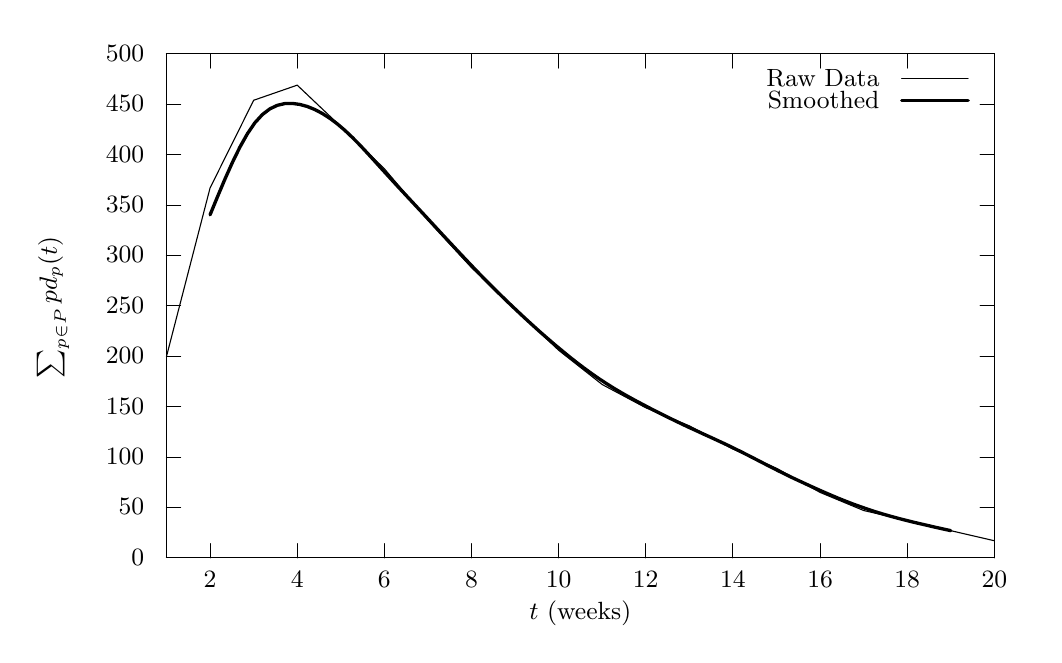
\begin{tikzpicture}[gnuplot]
%% generated with GNUPLOT 4.6p4 (Lua 5.1; terminal rev. 99, script rev. 100)
%% Thu 04 Sep 2014 10:50:27 WST
\tikzset{every node/.append style={font={\fontsize{9pt}{10.8pt}\selectfont}}}
\gpmonochromelines
\path (0.000,0.000) rectangle (12.700,7.620);
\gpcolor{color=gp lt color border}
\gpsetlinetype{gp lt border}
\gpsetlinewidth{1.00}
\draw[gp path] (1.688,0.886)--(1.868,0.886);
\draw[gp path] (12.201,0.886)--(12.021,0.886);
\node[gp node right] at (1.522,0.886) { 0};
\draw[gp path] (1.688,1.526)--(1.868,1.526);
\draw[gp path] (12.201,1.526)--(12.021,1.526);
\node[gp node right] at (1.522,1.526) { 50};
\draw[gp path] (1.688,2.166)--(1.868,2.166);
\draw[gp path] (12.201,2.166)--(12.021,2.166);
\node[gp node right] at (1.522,2.166) { 100};
\draw[gp path] (1.688,2.806)--(1.868,2.806);
\draw[gp path] (12.201,2.806)--(12.021,2.806);
\node[gp node right] at (1.522,2.806) { 150};
\draw[gp path] (1.688,3.446)--(1.868,3.446);
\draw[gp path] (12.201,3.446)--(12.021,3.446);
\node[gp node right] at (1.522,3.446) { 200};
\draw[gp path] (1.688,4.087)--(1.868,4.087);
\draw[gp path] (12.201,4.087)--(12.021,4.087);
\node[gp node right] at (1.522,4.087) { 250};
\draw[gp path] (1.688,4.727)--(1.868,4.727);
\draw[gp path] (12.201,4.727)--(12.021,4.727);
\node[gp node right] at (1.522,4.727) { 300};
\draw[gp path] (1.688,5.367)--(1.868,5.367);
\draw[gp path] (12.201,5.367)--(12.021,5.367);
\node[gp node right] at (1.522,5.367) { 350};
\draw[gp path] (1.688,6.007)--(1.868,6.007);
\draw[gp path] (12.201,6.007)--(12.021,6.007);
\node[gp node right] at (1.522,6.007) { 400};
\draw[gp path] (1.688,6.647)--(1.868,6.647);
\draw[gp path] (12.201,6.647)--(12.021,6.647);
\node[gp node right] at (1.522,6.647) { 450};
\draw[gp path] (1.688,7.287)--(1.868,7.287);
\draw[gp path] (12.201,7.287)--(12.021,7.287);
\node[gp node right] at (1.522,7.287) { 500};
\draw[gp path] (2.241,0.886)--(2.241,1.066);
\draw[gp path] (2.241,7.287)--(2.241,7.107);
\node[gp node center] at (2.241,0.609) { 2};
\draw[gp path] (3.348,0.886)--(3.348,1.066);
\draw[gp path] (3.348,7.287)--(3.348,7.107);
\node[gp node center] at (3.348,0.609) { 4};
\draw[gp path] (4.455,0.886)--(4.455,1.066);
\draw[gp path] (4.455,7.287)--(4.455,7.107);
\node[gp node center] at (4.455,0.609) { 6};
\draw[gp path] (5.561,0.886)--(5.561,1.066);
\draw[gp path] (5.561,7.287)--(5.561,7.107);
\node[gp node center] at (5.561,0.609) { 8};
\draw[gp path] (6.668,0.886)--(6.668,1.066);
\draw[gp path] (6.668,7.287)--(6.668,7.107);
\node[gp node center] at (6.668,0.609) { 10};
\draw[gp path] (7.774,0.886)--(7.774,1.066);
\draw[gp path] (7.774,7.287)--(7.774,7.107);
\node[gp node center] at (7.774,0.609) { 12};
\draw[gp path] (8.881,0.886)--(8.881,1.066);
\draw[gp path] (8.881,7.287)--(8.881,7.107);
\node[gp node center] at (8.881,0.609) { 14};
\draw[gp path] (9.988,0.886)--(9.988,1.066);
\draw[gp path] (9.988,7.287)--(9.988,7.107);
\node[gp node center] at (9.988,0.609) { 16};
\draw[gp path] (11.094,0.886)--(11.094,1.066);
\draw[gp path] (11.094,7.287)--(11.094,7.107);
\node[gp node center] at (11.094,0.609) { 18};
\draw[gp path] (12.201,0.886)--(12.201,1.066);
\draw[gp path] (12.201,7.287)--(12.201,7.107);
\node[gp node center] at (12.201,0.609) { 20};
\draw[gp path] (1.688,7.287)--(1.688,0.886)--(12.201,0.886)--(12.201,7.287)--cycle;
\node[gp node center,rotate=-270] at (0.221,4.086) {$\sum_{p \in P} p d_p(t)$};
\node[gp node center] at (6.944,0.194) {$t$ (weeks)};
\node[gp node right] at (10.859,6.969) {Raw Data};
\gpcolor{color=gp lt color 3}
\gpsetlinetype{gp lt plot 3}
\draw[gp path] (11.025,6.969)--(11.869,6.969);
\draw[gp path] (1.688,3.446)--(2.241,5.584)--(2.795,6.698)--(3.348,6.890)--(3.901,6.365)%
  --(4.455,5.828)--(5.008,5.175)--(5.561,4.573)--(6.115,4.048)--(6.668,3.523)--(7.221,3.088)%
  --(7.774,2.793)--(8.328,2.563)--(8.881,2.269)--(9.434,2.025)--(9.988,1.718)--(10.541,1.488)%
  --(11.094,1.360)--(11.648,1.232)--(12.201,1.104);
\gpcolor{color=gp lt color border}
\node[gp node right] at (10.859,6.692) {Smoothed};
\gpcolor{color=gp lt color 0}
\gpsetlinetype{gp lt plot 0}
\gpsetlinewidth{3.00}
\draw[gp path] (11.025,6.692)--(11.869,6.692);
\draw[gp path] (2.241,5.243)--(2.336,5.474)--(2.431,5.699)--(2.526,5.911)--(2.621,6.105)%
  --(2.716,6.274)--(2.811,6.413)--(2.906,6.517)--(3.001,6.589)--(3.096,6.634)--(3.191,6.656)%
  --(3.286,6.658)--(3.381,6.645)--(3.476,6.619)--(3.572,6.580)--(3.667,6.530)--(3.762,6.469)%
  --(3.857,6.398)--(3.952,6.317)--(4.047,6.227)--(4.142,6.131)--(4.237,6.029)--(4.332,5.925)%
  --(4.427,5.820)--(4.522,5.716)--(4.617,5.612)--(4.712,5.510)--(4.807,5.408)--(4.902,5.306)%
  --(4.997,5.204)--(5.092,5.101)--(5.187,4.998)--(5.282,4.896)--(5.377,4.794)--(5.472,4.693)%
  --(5.567,4.593)--(5.662,4.494)--(5.757,4.398)--(5.852,4.303)--(5.947,4.209)--(6.042,4.117)%
  --(6.137,4.027)--(6.232,3.938)--(6.327,3.851)--(6.422,3.765)--(6.517,3.682)--(6.612,3.600)%
  --(6.707,3.521)--(6.802,3.443)--(6.897,3.368)--(6.992,3.296)--(7.087,3.227)--(7.182,3.161)%
  --(7.277,3.099)--(7.372,3.039)--(7.467,2.983)--(7.562,2.929)--(7.657,2.877)--(7.752,2.827)%
  --(7.847,2.777)--(7.942,2.729)--(8.037,2.681)--(8.132,2.635)--(8.227,2.589)--(8.322,2.544)%
  --(8.417,2.501)--(8.512,2.457)--(8.607,2.414)--(8.702,2.370)--(8.797,2.326)--(8.892,2.280)%
  --(8.987,2.233)--(9.082,2.185)--(9.177,2.136)--(9.272,2.087)--(9.367,2.038)--(9.462,1.990)%
  --(9.557,1.943)--(9.652,1.897)--(9.747,1.853)--(9.842,1.809)--(9.937,1.766)--(10.032,1.724)%
  --(10.127,1.683)--(10.222,1.643)--(10.317,1.605)--(10.413,1.568)--(10.508,1.534)--(10.603,1.501)%
  --(10.698,1.470)--(10.793,1.441)--(10.888,1.414)--(10.983,1.388)--(11.078,1.364)--(11.173,1.340)%
  --(11.268,1.318)--(11.363,1.296)--(11.458,1.274)--(11.553,1.253)--(11.648,1.232);
\gpcolor{color=gp lt color border}
\gpsetlinetype{gp lt border}
\gpsetlinewidth{1.00}
\draw[gp path] (1.688,7.287)--(1.688,0.886)--(12.201,0.886)--(12.201,7.287)--cycle;
%% coordinates of the plot area
\gpdefrectangularnode{gp plot 1}{\pgfpoint{1.688cm}{0.886cm}}{\pgfpoint{12.201cm}{7.287cm}}
\end{tikzpicture}
%% gnuplot variables

    \caption{Easy--Hard, Major--Minor}
  \end{figure}
  
  \begin{figure}[!htb]
    \centering
    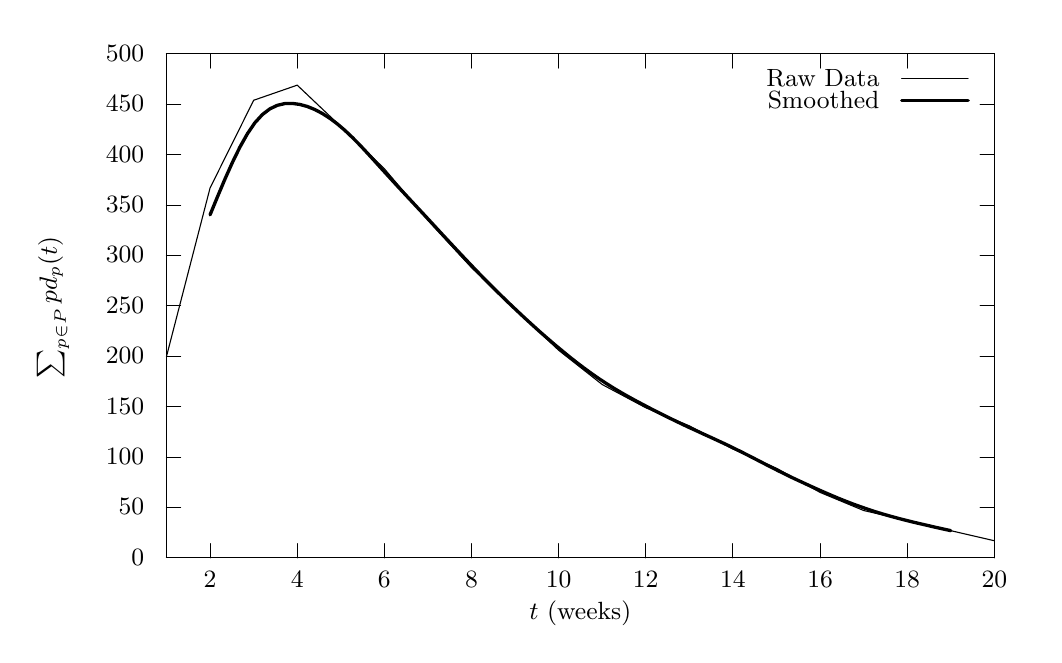
\begin{tikzpicture}[gnuplot]
%% generated with GNUPLOT 4.6p4 (Lua 5.1; terminal rev. 99, script rev. 100)
%% Thu 04 Sep 2014 10:50:27 WST
\tikzset{every node/.append style={font={\fontsize{9pt}{10.8pt}\selectfont}}}
\gpmonochromelines
\path (0.000,0.000) rectangle (12.700,7.620);
\gpcolor{color=gp lt color border}
\gpsetlinetype{gp lt border}
\gpsetlinewidth{1.00}
\draw[gp path] (1.688,0.886)--(1.868,0.886);
\draw[gp path] (12.201,0.886)--(12.021,0.886);
\node[gp node right] at (1.522,0.886) { 0};
\draw[gp path] (1.688,1.526)--(1.868,1.526);
\draw[gp path] (12.201,1.526)--(12.021,1.526);
\node[gp node right] at (1.522,1.526) { 50};
\draw[gp path] (1.688,2.166)--(1.868,2.166);
\draw[gp path] (12.201,2.166)--(12.021,2.166);
\node[gp node right] at (1.522,2.166) { 100};
\draw[gp path] (1.688,2.806)--(1.868,2.806);
\draw[gp path] (12.201,2.806)--(12.021,2.806);
\node[gp node right] at (1.522,2.806) { 150};
\draw[gp path] (1.688,3.446)--(1.868,3.446);
\draw[gp path] (12.201,3.446)--(12.021,3.446);
\node[gp node right] at (1.522,3.446) { 200};
\draw[gp path] (1.688,4.087)--(1.868,4.087);
\draw[gp path] (12.201,4.087)--(12.021,4.087);
\node[gp node right] at (1.522,4.087) { 250};
\draw[gp path] (1.688,4.727)--(1.868,4.727);
\draw[gp path] (12.201,4.727)--(12.021,4.727);
\node[gp node right] at (1.522,4.727) { 300};
\draw[gp path] (1.688,5.367)--(1.868,5.367);
\draw[gp path] (12.201,5.367)--(12.021,5.367);
\node[gp node right] at (1.522,5.367) { 350};
\draw[gp path] (1.688,6.007)--(1.868,6.007);
\draw[gp path] (12.201,6.007)--(12.021,6.007);
\node[gp node right] at (1.522,6.007) { 400};
\draw[gp path] (1.688,6.647)--(1.868,6.647);
\draw[gp path] (12.201,6.647)--(12.021,6.647);
\node[gp node right] at (1.522,6.647) { 450};
\draw[gp path] (1.688,7.287)--(1.868,7.287);
\draw[gp path] (12.201,7.287)--(12.021,7.287);
\node[gp node right] at (1.522,7.287) { 500};
\draw[gp path] (2.241,0.886)--(2.241,1.066);
\draw[gp path] (2.241,7.287)--(2.241,7.107);
\node[gp node center] at (2.241,0.609) { 2};
\draw[gp path] (3.348,0.886)--(3.348,1.066);
\draw[gp path] (3.348,7.287)--(3.348,7.107);
\node[gp node center] at (3.348,0.609) { 4};
\draw[gp path] (4.455,0.886)--(4.455,1.066);
\draw[gp path] (4.455,7.287)--(4.455,7.107);
\node[gp node center] at (4.455,0.609) { 6};
\draw[gp path] (5.561,0.886)--(5.561,1.066);
\draw[gp path] (5.561,7.287)--(5.561,7.107);
\node[gp node center] at (5.561,0.609) { 8};
\draw[gp path] (6.668,0.886)--(6.668,1.066);
\draw[gp path] (6.668,7.287)--(6.668,7.107);
\node[gp node center] at (6.668,0.609) { 10};
\draw[gp path] (7.774,0.886)--(7.774,1.066);
\draw[gp path] (7.774,7.287)--(7.774,7.107);
\node[gp node center] at (7.774,0.609) { 12};
\draw[gp path] (8.881,0.886)--(8.881,1.066);
\draw[gp path] (8.881,7.287)--(8.881,7.107);
\node[gp node center] at (8.881,0.609) { 14};
\draw[gp path] (9.988,0.886)--(9.988,1.066);
\draw[gp path] (9.988,7.287)--(9.988,7.107);
\node[gp node center] at (9.988,0.609) { 16};
\draw[gp path] (11.094,0.886)--(11.094,1.066);
\draw[gp path] (11.094,7.287)--(11.094,7.107);
\node[gp node center] at (11.094,0.609) { 18};
\draw[gp path] (12.201,0.886)--(12.201,1.066);
\draw[gp path] (12.201,7.287)--(12.201,7.107);
\node[gp node center] at (12.201,0.609) { 20};
\draw[gp path] (1.688,7.287)--(1.688,0.886)--(12.201,0.886)--(12.201,7.287)--cycle;
\node[gp node center,rotate=-270] at (0.221,4.086) {$\sum_{p \in P} p d_p(t)$};
\node[gp node center] at (6.944,0.194) {$t$ (weeks)};
\node[gp node right] at (10.859,6.969) {Raw Data};
\gpcolor{color=gp lt color 3}
\gpsetlinetype{gp lt plot 3}
\draw[gp path] (11.025,6.969)--(11.869,6.969);
\draw[gp path] (1.688,3.446)--(2.241,5.584)--(2.795,6.698)--(3.348,6.890)--(3.901,6.365)%
  --(4.455,5.828)--(5.008,5.175)--(5.561,4.573)--(6.115,4.048)--(6.668,3.523)--(7.221,3.088)%
  --(7.774,2.793)--(8.328,2.563)--(8.881,2.269)--(9.434,2.025)--(9.988,1.718)--(10.541,1.488)%
  --(11.094,1.360)--(11.648,1.232)--(12.201,1.104);
\gpcolor{color=gp lt color border}
\node[gp node right] at (10.859,6.692) {Smoothed};
\gpcolor{color=gp lt color 0}
\gpsetlinetype{gp lt plot 0}
\gpsetlinewidth{3.00}
\draw[gp path] (11.025,6.692)--(11.869,6.692);
\draw[gp path] (2.241,5.243)--(2.336,5.474)--(2.431,5.699)--(2.526,5.911)--(2.621,6.105)%
  --(2.716,6.274)--(2.811,6.413)--(2.906,6.517)--(3.001,6.589)--(3.096,6.634)--(3.191,6.656)%
  --(3.286,6.658)--(3.381,6.645)--(3.476,6.619)--(3.572,6.580)--(3.667,6.530)--(3.762,6.469)%
  --(3.857,6.398)--(3.952,6.317)--(4.047,6.227)--(4.142,6.131)--(4.237,6.029)--(4.332,5.925)%
  --(4.427,5.820)--(4.522,5.716)--(4.617,5.612)--(4.712,5.510)--(4.807,5.408)--(4.902,5.306)%
  --(4.997,5.204)--(5.092,5.101)--(5.187,4.998)--(5.282,4.896)--(5.377,4.794)--(5.472,4.693)%
  --(5.567,4.593)--(5.662,4.494)--(5.757,4.398)--(5.852,4.303)--(5.947,4.209)--(6.042,4.117)%
  --(6.137,4.027)--(6.232,3.938)--(6.327,3.851)--(6.422,3.765)--(6.517,3.682)--(6.612,3.600)%
  --(6.707,3.521)--(6.802,3.443)--(6.897,3.368)--(6.992,3.296)--(7.087,3.227)--(7.182,3.161)%
  --(7.277,3.099)--(7.372,3.039)--(7.467,2.983)--(7.562,2.929)--(7.657,2.877)--(7.752,2.827)%
  --(7.847,2.777)--(7.942,2.729)--(8.037,2.681)--(8.132,2.635)--(8.227,2.589)--(8.322,2.544)%
  --(8.417,2.501)--(8.512,2.457)--(8.607,2.414)--(8.702,2.370)--(8.797,2.326)--(8.892,2.280)%
  --(8.987,2.233)--(9.082,2.185)--(9.177,2.136)--(9.272,2.087)--(9.367,2.038)--(9.462,1.990)%
  --(9.557,1.943)--(9.652,1.897)--(9.747,1.853)--(9.842,1.809)--(9.937,1.766)--(10.032,1.724)%
  --(10.127,1.683)--(10.222,1.643)--(10.317,1.605)--(10.413,1.568)--(10.508,1.534)--(10.603,1.501)%
  --(10.698,1.470)--(10.793,1.441)--(10.888,1.414)--(10.983,1.388)--(11.078,1.364)--(11.173,1.340)%
  --(11.268,1.318)--(11.363,1.296)--(11.458,1.274)--(11.553,1.253)--(11.648,1.232);
\gpcolor{color=gp lt color border}
\gpsetlinetype{gp lt border}
\gpsetlinewidth{1.00}
\draw[gp path] (1.688,7.287)--(1.688,0.886)--(12.201,0.886)--(12.201,7.287)--cycle;
%% coordinates of the plot area
\gpdefrectangularnode{gp plot 1}{\pgfpoint{1.688cm}{0.886cm}}{\pgfpoint{12.201cm}{7.287cm}}
\end{tikzpicture}
%% gnuplot variables

    \caption{Hard--Easy, Major--Minor}
  \end{figure}
  
  \begin{figure}[!htb]
    \centering
    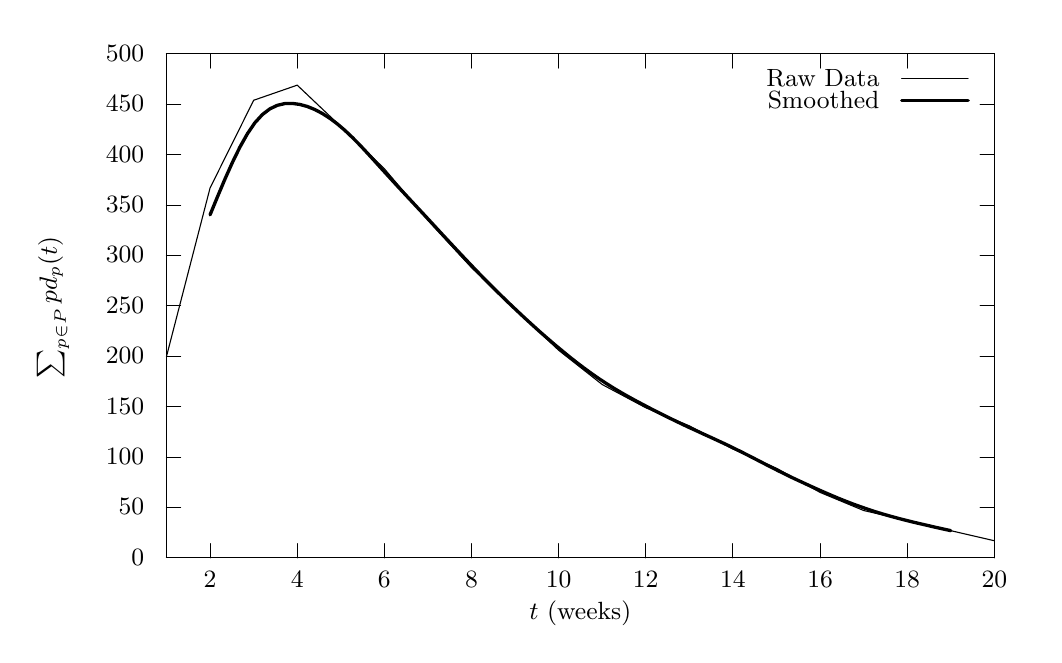
\begin{tikzpicture}[gnuplot]
%% generated with GNUPLOT 4.6p4 (Lua 5.1; terminal rev. 99, script rev. 100)
%% Thu 04 Sep 2014 10:50:27 WST
\tikzset{every node/.append style={font={\fontsize{9pt}{10.8pt}\selectfont}}}
\gpmonochromelines
\path (0.000,0.000) rectangle (12.700,7.620);
\gpcolor{color=gp lt color border}
\gpsetlinetype{gp lt border}
\gpsetlinewidth{1.00}
\draw[gp path] (1.688,0.886)--(1.868,0.886);
\draw[gp path] (12.201,0.886)--(12.021,0.886);
\node[gp node right] at (1.522,0.886) { 0};
\draw[gp path] (1.688,1.526)--(1.868,1.526);
\draw[gp path] (12.201,1.526)--(12.021,1.526);
\node[gp node right] at (1.522,1.526) { 50};
\draw[gp path] (1.688,2.166)--(1.868,2.166);
\draw[gp path] (12.201,2.166)--(12.021,2.166);
\node[gp node right] at (1.522,2.166) { 100};
\draw[gp path] (1.688,2.806)--(1.868,2.806);
\draw[gp path] (12.201,2.806)--(12.021,2.806);
\node[gp node right] at (1.522,2.806) { 150};
\draw[gp path] (1.688,3.446)--(1.868,3.446);
\draw[gp path] (12.201,3.446)--(12.021,3.446);
\node[gp node right] at (1.522,3.446) { 200};
\draw[gp path] (1.688,4.087)--(1.868,4.087);
\draw[gp path] (12.201,4.087)--(12.021,4.087);
\node[gp node right] at (1.522,4.087) { 250};
\draw[gp path] (1.688,4.727)--(1.868,4.727);
\draw[gp path] (12.201,4.727)--(12.021,4.727);
\node[gp node right] at (1.522,4.727) { 300};
\draw[gp path] (1.688,5.367)--(1.868,5.367);
\draw[gp path] (12.201,5.367)--(12.021,5.367);
\node[gp node right] at (1.522,5.367) { 350};
\draw[gp path] (1.688,6.007)--(1.868,6.007);
\draw[gp path] (12.201,6.007)--(12.021,6.007);
\node[gp node right] at (1.522,6.007) { 400};
\draw[gp path] (1.688,6.647)--(1.868,6.647);
\draw[gp path] (12.201,6.647)--(12.021,6.647);
\node[gp node right] at (1.522,6.647) { 450};
\draw[gp path] (1.688,7.287)--(1.868,7.287);
\draw[gp path] (12.201,7.287)--(12.021,7.287);
\node[gp node right] at (1.522,7.287) { 500};
\draw[gp path] (2.241,0.886)--(2.241,1.066);
\draw[gp path] (2.241,7.287)--(2.241,7.107);
\node[gp node center] at (2.241,0.609) { 2};
\draw[gp path] (3.348,0.886)--(3.348,1.066);
\draw[gp path] (3.348,7.287)--(3.348,7.107);
\node[gp node center] at (3.348,0.609) { 4};
\draw[gp path] (4.455,0.886)--(4.455,1.066);
\draw[gp path] (4.455,7.287)--(4.455,7.107);
\node[gp node center] at (4.455,0.609) { 6};
\draw[gp path] (5.561,0.886)--(5.561,1.066);
\draw[gp path] (5.561,7.287)--(5.561,7.107);
\node[gp node center] at (5.561,0.609) { 8};
\draw[gp path] (6.668,0.886)--(6.668,1.066);
\draw[gp path] (6.668,7.287)--(6.668,7.107);
\node[gp node center] at (6.668,0.609) { 10};
\draw[gp path] (7.774,0.886)--(7.774,1.066);
\draw[gp path] (7.774,7.287)--(7.774,7.107);
\node[gp node center] at (7.774,0.609) { 12};
\draw[gp path] (8.881,0.886)--(8.881,1.066);
\draw[gp path] (8.881,7.287)--(8.881,7.107);
\node[gp node center] at (8.881,0.609) { 14};
\draw[gp path] (9.988,0.886)--(9.988,1.066);
\draw[gp path] (9.988,7.287)--(9.988,7.107);
\node[gp node center] at (9.988,0.609) { 16};
\draw[gp path] (11.094,0.886)--(11.094,1.066);
\draw[gp path] (11.094,7.287)--(11.094,7.107);
\node[gp node center] at (11.094,0.609) { 18};
\draw[gp path] (12.201,0.886)--(12.201,1.066);
\draw[gp path] (12.201,7.287)--(12.201,7.107);
\node[gp node center] at (12.201,0.609) { 20};
\draw[gp path] (1.688,7.287)--(1.688,0.886)--(12.201,0.886)--(12.201,7.287)--cycle;
\node[gp node center,rotate=-270] at (0.221,4.086) {$\sum_{p \in P} p d_p(t)$};
\node[gp node center] at (6.944,0.194) {$t$ (weeks)};
\node[gp node right] at (10.859,6.969) {Raw Data};
\gpcolor{color=gp lt color 3}
\gpsetlinetype{gp lt plot 3}
\draw[gp path] (11.025,6.969)--(11.869,6.969);
\draw[gp path] (1.688,3.446)--(2.241,5.584)--(2.795,6.698)--(3.348,6.890)--(3.901,6.365)%
  --(4.455,5.828)--(5.008,5.175)--(5.561,4.573)--(6.115,4.048)--(6.668,3.523)--(7.221,3.088)%
  --(7.774,2.793)--(8.328,2.563)--(8.881,2.269)--(9.434,2.025)--(9.988,1.718)--(10.541,1.488)%
  --(11.094,1.360)--(11.648,1.232)--(12.201,1.104);
\gpcolor{color=gp lt color border}
\node[gp node right] at (10.859,6.692) {Smoothed};
\gpcolor{color=gp lt color 0}
\gpsetlinetype{gp lt plot 0}
\gpsetlinewidth{3.00}
\draw[gp path] (11.025,6.692)--(11.869,6.692);
\draw[gp path] (2.241,5.243)--(2.336,5.474)--(2.431,5.699)--(2.526,5.911)--(2.621,6.105)%
  --(2.716,6.274)--(2.811,6.413)--(2.906,6.517)--(3.001,6.589)--(3.096,6.634)--(3.191,6.656)%
  --(3.286,6.658)--(3.381,6.645)--(3.476,6.619)--(3.572,6.580)--(3.667,6.530)--(3.762,6.469)%
  --(3.857,6.398)--(3.952,6.317)--(4.047,6.227)--(4.142,6.131)--(4.237,6.029)--(4.332,5.925)%
  --(4.427,5.820)--(4.522,5.716)--(4.617,5.612)--(4.712,5.510)--(4.807,5.408)--(4.902,5.306)%
  --(4.997,5.204)--(5.092,5.101)--(5.187,4.998)--(5.282,4.896)--(5.377,4.794)--(5.472,4.693)%
  --(5.567,4.593)--(5.662,4.494)--(5.757,4.398)--(5.852,4.303)--(5.947,4.209)--(6.042,4.117)%
  --(6.137,4.027)--(6.232,3.938)--(6.327,3.851)--(6.422,3.765)--(6.517,3.682)--(6.612,3.600)%
  --(6.707,3.521)--(6.802,3.443)--(6.897,3.368)--(6.992,3.296)--(7.087,3.227)--(7.182,3.161)%
  --(7.277,3.099)--(7.372,3.039)--(7.467,2.983)--(7.562,2.929)--(7.657,2.877)--(7.752,2.827)%
  --(7.847,2.777)--(7.942,2.729)--(8.037,2.681)--(8.132,2.635)--(8.227,2.589)--(8.322,2.544)%
  --(8.417,2.501)--(8.512,2.457)--(8.607,2.414)--(8.702,2.370)--(8.797,2.326)--(8.892,2.280)%
  --(8.987,2.233)--(9.082,2.185)--(9.177,2.136)--(9.272,2.087)--(9.367,2.038)--(9.462,1.990)%
  --(9.557,1.943)--(9.652,1.897)--(9.747,1.853)--(9.842,1.809)--(9.937,1.766)--(10.032,1.724)%
  --(10.127,1.683)--(10.222,1.643)--(10.317,1.605)--(10.413,1.568)--(10.508,1.534)--(10.603,1.501)%
  --(10.698,1.470)--(10.793,1.441)--(10.888,1.414)--(10.983,1.388)--(11.078,1.364)--(11.173,1.340)%
  --(11.268,1.318)--(11.363,1.296)--(11.458,1.274)--(11.553,1.253)--(11.648,1.232);
\gpcolor{color=gp lt color border}
\gpsetlinetype{gp lt border}
\gpsetlinewidth{1.00}
\draw[gp path] (1.688,7.287)--(1.688,0.886)--(12.201,0.886)--(12.201,7.287)--cycle;
%% coordinates of the plot area
\gpdefrectangularnode{gp plot 1}{\pgfpoint{1.688cm}{0.886cm}}{\pgfpoint{12.201cm}{7.287cm}}
\end{tikzpicture}
%% gnuplot variables

    \caption{Major--Minor, Easy--Hard}
  \end{figure}
  
  \begin{figure}[!htb]
    \centering
    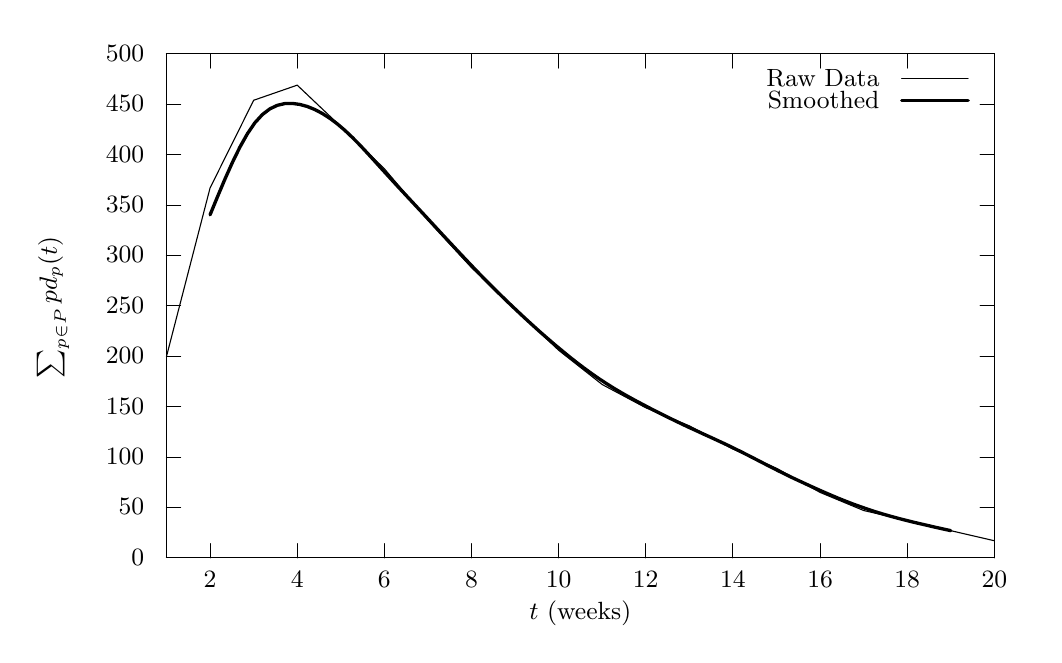
\begin{tikzpicture}[gnuplot]
%% generated with GNUPLOT 4.6p4 (Lua 5.1; terminal rev. 99, script rev. 100)
%% Thu 04 Sep 2014 10:50:27 WST
\tikzset{every node/.append style={font={\fontsize{9pt}{10.8pt}\selectfont}}}
\gpmonochromelines
\path (0.000,0.000) rectangle (12.700,7.620);
\gpcolor{color=gp lt color border}
\gpsetlinetype{gp lt border}
\gpsetlinewidth{1.00}
\draw[gp path] (1.688,0.886)--(1.868,0.886);
\draw[gp path] (12.201,0.886)--(12.021,0.886);
\node[gp node right] at (1.522,0.886) { 0};
\draw[gp path] (1.688,1.526)--(1.868,1.526);
\draw[gp path] (12.201,1.526)--(12.021,1.526);
\node[gp node right] at (1.522,1.526) { 50};
\draw[gp path] (1.688,2.166)--(1.868,2.166);
\draw[gp path] (12.201,2.166)--(12.021,2.166);
\node[gp node right] at (1.522,2.166) { 100};
\draw[gp path] (1.688,2.806)--(1.868,2.806);
\draw[gp path] (12.201,2.806)--(12.021,2.806);
\node[gp node right] at (1.522,2.806) { 150};
\draw[gp path] (1.688,3.446)--(1.868,3.446);
\draw[gp path] (12.201,3.446)--(12.021,3.446);
\node[gp node right] at (1.522,3.446) { 200};
\draw[gp path] (1.688,4.087)--(1.868,4.087);
\draw[gp path] (12.201,4.087)--(12.021,4.087);
\node[gp node right] at (1.522,4.087) { 250};
\draw[gp path] (1.688,4.727)--(1.868,4.727);
\draw[gp path] (12.201,4.727)--(12.021,4.727);
\node[gp node right] at (1.522,4.727) { 300};
\draw[gp path] (1.688,5.367)--(1.868,5.367);
\draw[gp path] (12.201,5.367)--(12.021,5.367);
\node[gp node right] at (1.522,5.367) { 350};
\draw[gp path] (1.688,6.007)--(1.868,6.007);
\draw[gp path] (12.201,6.007)--(12.021,6.007);
\node[gp node right] at (1.522,6.007) { 400};
\draw[gp path] (1.688,6.647)--(1.868,6.647);
\draw[gp path] (12.201,6.647)--(12.021,6.647);
\node[gp node right] at (1.522,6.647) { 450};
\draw[gp path] (1.688,7.287)--(1.868,7.287);
\draw[gp path] (12.201,7.287)--(12.021,7.287);
\node[gp node right] at (1.522,7.287) { 500};
\draw[gp path] (2.241,0.886)--(2.241,1.066);
\draw[gp path] (2.241,7.287)--(2.241,7.107);
\node[gp node center] at (2.241,0.609) { 2};
\draw[gp path] (3.348,0.886)--(3.348,1.066);
\draw[gp path] (3.348,7.287)--(3.348,7.107);
\node[gp node center] at (3.348,0.609) { 4};
\draw[gp path] (4.455,0.886)--(4.455,1.066);
\draw[gp path] (4.455,7.287)--(4.455,7.107);
\node[gp node center] at (4.455,0.609) { 6};
\draw[gp path] (5.561,0.886)--(5.561,1.066);
\draw[gp path] (5.561,7.287)--(5.561,7.107);
\node[gp node center] at (5.561,0.609) { 8};
\draw[gp path] (6.668,0.886)--(6.668,1.066);
\draw[gp path] (6.668,7.287)--(6.668,7.107);
\node[gp node center] at (6.668,0.609) { 10};
\draw[gp path] (7.774,0.886)--(7.774,1.066);
\draw[gp path] (7.774,7.287)--(7.774,7.107);
\node[gp node center] at (7.774,0.609) { 12};
\draw[gp path] (8.881,0.886)--(8.881,1.066);
\draw[gp path] (8.881,7.287)--(8.881,7.107);
\node[gp node center] at (8.881,0.609) { 14};
\draw[gp path] (9.988,0.886)--(9.988,1.066);
\draw[gp path] (9.988,7.287)--(9.988,7.107);
\node[gp node center] at (9.988,0.609) { 16};
\draw[gp path] (11.094,0.886)--(11.094,1.066);
\draw[gp path] (11.094,7.287)--(11.094,7.107);
\node[gp node center] at (11.094,0.609) { 18};
\draw[gp path] (12.201,0.886)--(12.201,1.066);
\draw[gp path] (12.201,7.287)--(12.201,7.107);
\node[gp node center] at (12.201,0.609) { 20};
\draw[gp path] (1.688,7.287)--(1.688,0.886)--(12.201,0.886)--(12.201,7.287)--cycle;
\node[gp node center,rotate=-270] at (0.221,4.086) {$\sum_{p \in P} p d_p(t)$};
\node[gp node center] at (6.944,0.194) {$t$ (weeks)};
\node[gp node right] at (10.859,6.969) {Raw Data};
\gpcolor{color=gp lt color 3}
\gpsetlinetype{gp lt plot 3}
\draw[gp path] (11.025,6.969)--(11.869,6.969);
\draw[gp path] (1.688,3.446)--(2.241,5.584)--(2.795,6.698)--(3.348,6.890)--(3.901,6.365)%
  --(4.455,5.828)--(5.008,5.175)--(5.561,4.573)--(6.115,4.048)--(6.668,3.523)--(7.221,3.088)%
  --(7.774,2.793)--(8.328,2.563)--(8.881,2.269)--(9.434,2.025)--(9.988,1.718)--(10.541,1.488)%
  --(11.094,1.360)--(11.648,1.232)--(12.201,1.104);
\gpcolor{color=gp lt color border}
\node[gp node right] at (10.859,6.692) {Smoothed};
\gpcolor{color=gp lt color 0}
\gpsetlinetype{gp lt plot 0}
\gpsetlinewidth{3.00}
\draw[gp path] (11.025,6.692)--(11.869,6.692);
\draw[gp path] (2.241,5.243)--(2.336,5.474)--(2.431,5.699)--(2.526,5.911)--(2.621,6.105)%
  --(2.716,6.274)--(2.811,6.413)--(2.906,6.517)--(3.001,6.589)--(3.096,6.634)--(3.191,6.656)%
  --(3.286,6.658)--(3.381,6.645)--(3.476,6.619)--(3.572,6.580)--(3.667,6.530)--(3.762,6.469)%
  --(3.857,6.398)--(3.952,6.317)--(4.047,6.227)--(4.142,6.131)--(4.237,6.029)--(4.332,5.925)%
  --(4.427,5.820)--(4.522,5.716)--(4.617,5.612)--(4.712,5.510)--(4.807,5.408)--(4.902,5.306)%
  --(4.997,5.204)--(5.092,5.101)--(5.187,4.998)--(5.282,4.896)--(5.377,4.794)--(5.472,4.693)%
  --(5.567,4.593)--(5.662,4.494)--(5.757,4.398)--(5.852,4.303)--(5.947,4.209)--(6.042,4.117)%
  --(6.137,4.027)--(6.232,3.938)--(6.327,3.851)--(6.422,3.765)--(6.517,3.682)--(6.612,3.600)%
  --(6.707,3.521)--(6.802,3.443)--(6.897,3.368)--(6.992,3.296)--(7.087,3.227)--(7.182,3.161)%
  --(7.277,3.099)--(7.372,3.039)--(7.467,2.983)--(7.562,2.929)--(7.657,2.877)--(7.752,2.827)%
  --(7.847,2.777)--(7.942,2.729)--(8.037,2.681)--(8.132,2.635)--(8.227,2.589)--(8.322,2.544)%
  --(8.417,2.501)--(8.512,2.457)--(8.607,2.414)--(8.702,2.370)--(8.797,2.326)--(8.892,2.280)%
  --(8.987,2.233)--(9.082,2.185)--(9.177,2.136)--(9.272,2.087)--(9.367,2.038)--(9.462,1.990)%
  --(9.557,1.943)--(9.652,1.897)--(9.747,1.853)--(9.842,1.809)--(9.937,1.766)--(10.032,1.724)%
  --(10.127,1.683)--(10.222,1.643)--(10.317,1.605)--(10.413,1.568)--(10.508,1.534)--(10.603,1.501)%
  --(10.698,1.470)--(10.793,1.441)--(10.888,1.414)--(10.983,1.388)--(11.078,1.364)--(11.173,1.340)%
  --(11.268,1.318)--(11.363,1.296)--(11.458,1.274)--(11.553,1.253)--(11.648,1.232);
\gpcolor{color=gp lt color border}
\gpsetlinetype{gp lt border}
\gpsetlinewidth{1.00}
\draw[gp path] (1.688,7.287)--(1.688,0.886)--(12.201,0.886)--(12.201,7.287)--cycle;
%% coordinates of the plot area
\gpdefrectangularnode{gp plot 1}{\pgfpoint{1.688cm}{0.886cm}}{\pgfpoint{12.201cm}{7.287cm}}
\end{tikzpicture}
%% gnuplot variables

    \caption{Minor--Major, Easy--Hard}
  \end{figure}
  
  \begin{figure}[!htb]
    \centering
    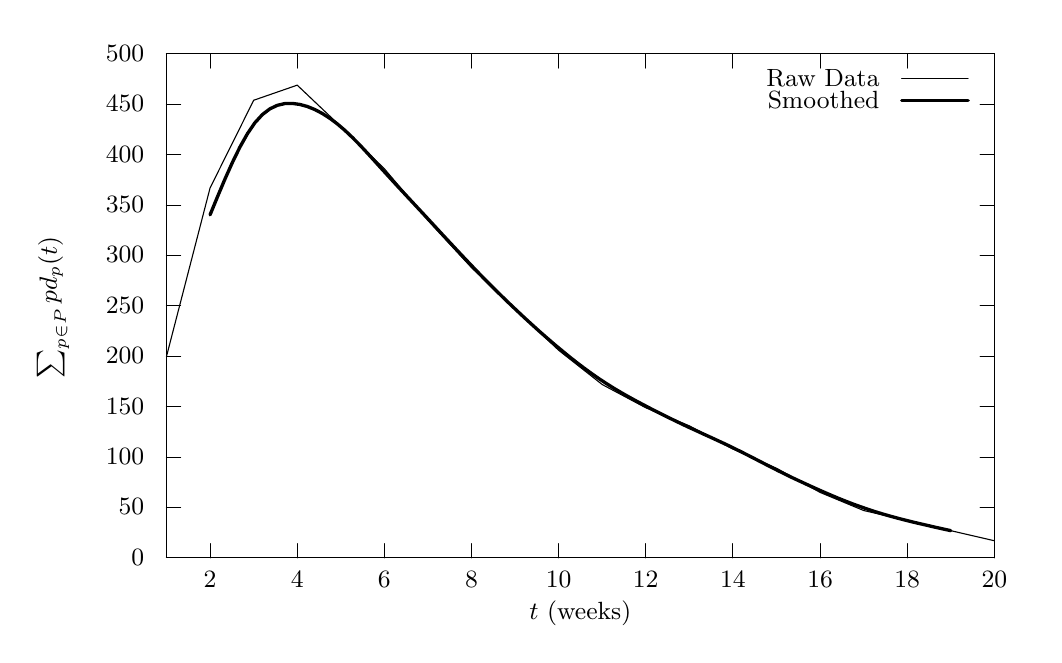
\begin{tikzpicture}[gnuplot]
%% generated with GNUPLOT 4.6p4 (Lua 5.1; terminal rev. 99, script rev. 100)
%% Thu 04 Sep 2014 10:50:27 WST
\tikzset{every node/.append style={font={\fontsize{9pt}{10.8pt}\selectfont}}}
\gpmonochromelines
\path (0.000,0.000) rectangle (12.700,7.620);
\gpcolor{color=gp lt color border}
\gpsetlinetype{gp lt border}
\gpsetlinewidth{1.00}
\draw[gp path] (1.688,0.886)--(1.868,0.886);
\draw[gp path] (12.201,0.886)--(12.021,0.886);
\node[gp node right] at (1.522,0.886) { 0};
\draw[gp path] (1.688,1.526)--(1.868,1.526);
\draw[gp path] (12.201,1.526)--(12.021,1.526);
\node[gp node right] at (1.522,1.526) { 50};
\draw[gp path] (1.688,2.166)--(1.868,2.166);
\draw[gp path] (12.201,2.166)--(12.021,2.166);
\node[gp node right] at (1.522,2.166) { 100};
\draw[gp path] (1.688,2.806)--(1.868,2.806);
\draw[gp path] (12.201,2.806)--(12.021,2.806);
\node[gp node right] at (1.522,2.806) { 150};
\draw[gp path] (1.688,3.446)--(1.868,3.446);
\draw[gp path] (12.201,3.446)--(12.021,3.446);
\node[gp node right] at (1.522,3.446) { 200};
\draw[gp path] (1.688,4.087)--(1.868,4.087);
\draw[gp path] (12.201,4.087)--(12.021,4.087);
\node[gp node right] at (1.522,4.087) { 250};
\draw[gp path] (1.688,4.727)--(1.868,4.727);
\draw[gp path] (12.201,4.727)--(12.021,4.727);
\node[gp node right] at (1.522,4.727) { 300};
\draw[gp path] (1.688,5.367)--(1.868,5.367);
\draw[gp path] (12.201,5.367)--(12.021,5.367);
\node[gp node right] at (1.522,5.367) { 350};
\draw[gp path] (1.688,6.007)--(1.868,6.007);
\draw[gp path] (12.201,6.007)--(12.021,6.007);
\node[gp node right] at (1.522,6.007) { 400};
\draw[gp path] (1.688,6.647)--(1.868,6.647);
\draw[gp path] (12.201,6.647)--(12.021,6.647);
\node[gp node right] at (1.522,6.647) { 450};
\draw[gp path] (1.688,7.287)--(1.868,7.287);
\draw[gp path] (12.201,7.287)--(12.021,7.287);
\node[gp node right] at (1.522,7.287) { 500};
\draw[gp path] (2.241,0.886)--(2.241,1.066);
\draw[gp path] (2.241,7.287)--(2.241,7.107);
\node[gp node center] at (2.241,0.609) { 2};
\draw[gp path] (3.348,0.886)--(3.348,1.066);
\draw[gp path] (3.348,7.287)--(3.348,7.107);
\node[gp node center] at (3.348,0.609) { 4};
\draw[gp path] (4.455,0.886)--(4.455,1.066);
\draw[gp path] (4.455,7.287)--(4.455,7.107);
\node[gp node center] at (4.455,0.609) { 6};
\draw[gp path] (5.561,0.886)--(5.561,1.066);
\draw[gp path] (5.561,7.287)--(5.561,7.107);
\node[gp node center] at (5.561,0.609) { 8};
\draw[gp path] (6.668,0.886)--(6.668,1.066);
\draw[gp path] (6.668,7.287)--(6.668,7.107);
\node[gp node center] at (6.668,0.609) { 10};
\draw[gp path] (7.774,0.886)--(7.774,1.066);
\draw[gp path] (7.774,7.287)--(7.774,7.107);
\node[gp node center] at (7.774,0.609) { 12};
\draw[gp path] (8.881,0.886)--(8.881,1.066);
\draw[gp path] (8.881,7.287)--(8.881,7.107);
\node[gp node center] at (8.881,0.609) { 14};
\draw[gp path] (9.988,0.886)--(9.988,1.066);
\draw[gp path] (9.988,7.287)--(9.988,7.107);
\node[gp node center] at (9.988,0.609) { 16};
\draw[gp path] (11.094,0.886)--(11.094,1.066);
\draw[gp path] (11.094,7.287)--(11.094,7.107);
\node[gp node center] at (11.094,0.609) { 18};
\draw[gp path] (12.201,0.886)--(12.201,1.066);
\draw[gp path] (12.201,7.287)--(12.201,7.107);
\node[gp node center] at (12.201,0.609) { 20};
\draw[gp path] (1.688,7.287)--(1.688,0.886)--(12.201,0.886)--(12.201,7.287)--cycle;
\node[gp node center,rotate=-270] at (0.221,4.086) {$\sum_{p \in P} p d_p(t)$};
\node[gp node center] at (6.944,0.194) {$t$ (weeks)};
\node[gp node right] at (10.859,6.969) {Raw Data};
\gpcolor{color=gp lt color 3}
\gpsetlinetype{gp lt plot 3}
\draw[gp path] (11.025,6.969)--(11.869,6.969);
\draw[gp path] (1.688,3.446)--(2.241,5.584)--(2.795,6.698)--(3.348,6.890)--(3.901,6.365)%
  --(4.455,5.828)--(5.008,5.175)--(5.561,4.573)--(6.115,4.048)--(6.668,3.523)--(7.221,3.088)%
  --(7.774,2.793)--(8.328,2.563)--(8.881,2.269)--(9.434,2.025)--(9.988,1.718)--(10.541,1.488)%
  --(11.094,1.360)--(11.648,1.232)--(12.201,1.104);
\gpcolor{color=gp lt color border}
\node[gp node right] at (10.859,6.692) {Smoothed};
\gpcolor{color=gp lt color 0}
\gpsetlinetype{gp lt plot 0}
\gpsetlinewidth{3.00}
\draw[gp path] (11.025,6.692)--(11.869,6.692);
\draw[gp path] (2.241,5.243)--(2.336,5.474)--(2.431,5.699)--(2.526,5.911)--(2.621,6.105)%
  --(2.716,6.274)--(2.811,6.413)--(2.906,6.517)--(3.001,6.589)--(3.096,6.634)--(3.191,6.656)%
  --(3.286,6.658)--(3.381,6.645)--(3.476,6.619)--(3.572,6.580)--(3.667,6.530)--(3.762,6.469)%
  --(3.857,6.398)--(3.952,6.317)--(4.047,6.227)--(4.142,6.131)--(4.237,6.029)--(4.332,5.925)%
  --(4.427,5.820)--(4.522,5.716)--(4.617,5.612)--(4.712,5.510)--(4.807,5.408)--(4.902,5.306)%
  --(4.997,5.204)--(5.092,5.101)--(5.187,4.998)--(5.282,4.896)--(5.377,4.794)--(5.472,4.693)%
  --(5.567,4.593)--(5.662,4.494)--(5.757,4.398)--(5.852,4.303)--(5.947,4.209)--(6.042,4.117)%
  --(6.137,4.027)--(6.232,3.938)--(6.327,3.851)--(6.422,3.765)--(6.517,3.682)--(6.612,3.600)%
  --(6.707,3.521)--(6.802,3.443)--(6.897,3.368)--(6.992,3.296)--(7.087,3.227)--(7.182,3.161)%
  --(7.277,3.099)--(7.372,3.039)--(7.467,2.983)--(7.562,2.929)--(7.657,2.877)--(7.752,2.827)%
  --(7.847,2.777)--(7.942,2.729)--(8.037,2.681)--(8.132,2.635)--(8.227,2.589)--(8.322,2.544)%
  --(8.417,2.501)--(8.512,2.457)--(8.607,2.414)--(8.702,2.370)--(8.797,2.326)--(8.892,2.280)%
  --(8.987,2.233)--(9.082,2.185)--(9.177,2.136)--(9.272,2.087)--(9.367,2.038)--(9.462,1.990)%
  --(9.557,1.943)--(9.652,1.897)--(9.747,1.853)--(9.842,1.809)--(9.937,1.766)--(10.032,1.724)%
  --(10.127,1.683)--(10.222,1.643)--(10.317,1.605)--(10.413,1.568)--(10.508,1.534)--(10.603,1.501)%
  --(10.698,1.470)--(10.793,1.441)--(10.888,1.414)--(10.983,1.388)--(11.078,1.364)--(11.173,1.340)%
  --(11.268,1.318)--(11.363,1.296)--(11.458,1.274)--(11.553,1.253)--(11.648,1.232);
\gpcolor{color=gp lt color border}
\gpsetlinetype{gp lt border}
\gpsetlinewidth{1.00}
\draw[gp path] (1.688,7.287)--(1.688,0.886)--(12.201,0.886)--(12.201,7.287)--cycle;
%% coordinates of the plot area
\gpdefrectangularnode{gp plot 1}{\pgfpoint{1.688cm}{0.886cm}}{\pgfpoint{12.201cm}{7.287cm}}
\end{tikzpicture}
%% gnuplot variables

    \caption{Random}
  \end{figure}
  
  \begin{figure}[!htb]
    \centering
    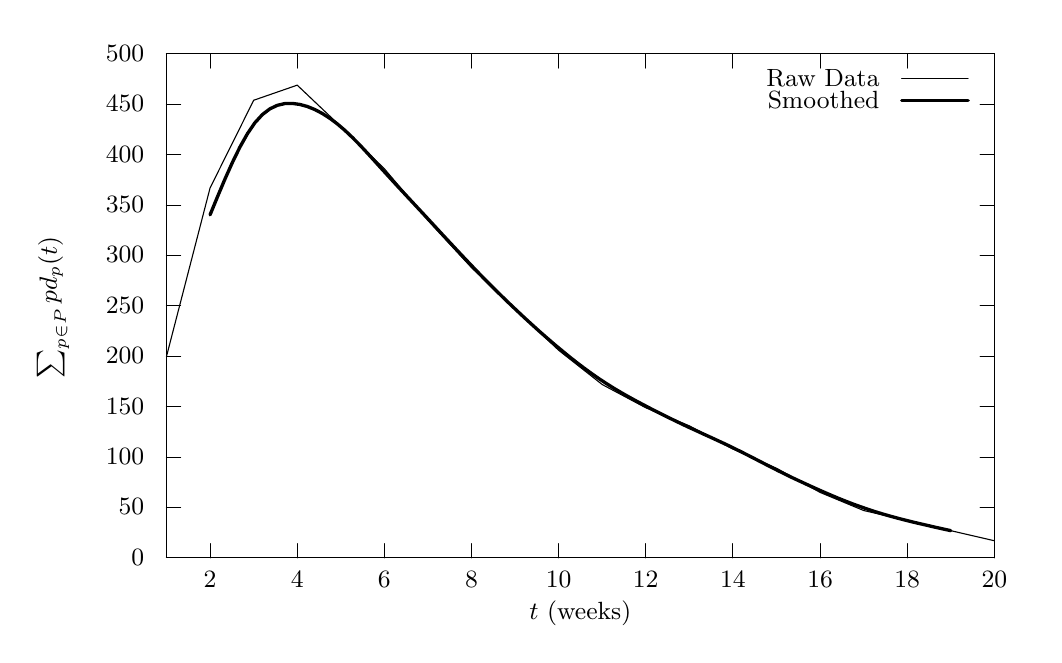
\begin{tikzpicture}[gnuplot]
%% generated with GNUPLOT 4.6p4 (Lua 5.1; terminal rev. 99, script rev. 100)
%% Thu 04 Sep 2014 10:50:27 WST
\tikzset{every node/.append style={font={\fontsize{9pt}{10.8pt}\selectfont}}}
\gpmonochromelines
\path (0.000,0.000) rectangle (12.700,7.620);
\gpcolor{color=gp lt color border}
\gpsetlinetype{gp lt border}
\gpsetlinewidth{1.00}
\draw[gp path] (1.688,0.886)--(1.868,0.886);
\draw[gp path] (12.201,0.886)--(12.021,0.886);
\node[gp node right] at (1.522,0.886) { 0};
\draw[gp path] (1.688,1.526)--(1.868,1.526);
\draw[gp path] (12.201,1.526)--(12.021,1.526);
\node[gp node right] at (1.522,1.526) { 50};
\draw[gp path] (1.688,2.166)--(1.868,2.166);
\draw[gp path] (12.201,2.166)--(12.021,2.166);
\node[gp node right] at (1.522,2.166) { 100};
\draw[gp path] (1.688,2.806)--(1.868,2.806);
\draw[gp path] (12.201,2.806)--(12.021,2.806);
\node[gp node right] at (1.522,2.806) { 150};
\draw[gp path] (1.688,3.446)--(1.868,3.446);
\draw[gp path] (12.201,3.446)--(12.021,3.446);
\node[gp node right] at (1.522,3.446) { 200};
\draw[gp path] (1.688,4.087)--(1.868,4.087);
\draw[gp path] (12.201,4.087)--(12.021,4.087);
\node[gp node right] at (1.522,4.087) { 250};
\draw[gp path] (1.688,4.727)--(1.868,4.727);
\draw[gp path] (12.201,4.727)--(12.021,4.727);
\node[gp node right] at (1.522,4.727) { 300};
\draw[gp path] (1.688,5.367)--(1.868,5.367);
\draw[gp path] (12.201,5.367)--(12.021,5.367);
\node[gp node right] at (1.522,5.367) { 350};
\draw[gp path] (1.688,6.007)--(1.868,6.007);
\draw[gp path] (12.201,6.007)--(12.021,6.007);
\node[gp node right] at (1.522,6.007) { 400};
\draw[gp path] (1.688,6.647)--(1.868,6.647);
\draw[gp path] (12.201,6.647)--(12.021,6.647);
\node[gp node right] at (1.522,6.647) { 450};
\draw[gp path] (1.688,7.287)--(1.868,7.287);
\draw[gp path] (12.201,7.287)--(12.021,7.287);
\node[gp node right] at (1.522,7.287) { 500};
\draw[gp path] (2.241,0.886)--(2.241,1.066);
\draw[gp path] (2.241,7.287)--(2.241,7.107);
\node[gp node center] at (2.241,0.609) { 2};
\draw[gp path] (3.348,0.886)--(3.348,1.066);
\draw[gp path] (3.348,7.287)--(3.348,7.107);
\node[gp node center] at (3.348,0.609) { 4};
\draw[gp path] (4.455,0.886)--(4.455,1.066);
\draw[gp path] (4.455,7.287)--(4.455,7.107);
\node[gp node center] at (4.455,0.609) { 6};
\draw[gp path] (5.561,0.886)--(5.561,1.066);
\draw[gp path] (5.561,7.287)--(5.561,7.107);
\node[gp node center] at (5.561,0.609) { 8};
\draw[gp path] (6.668,0.886)--(6.668,1.066);
\draw[gp path] (6.668,7.287)--(6.668,7.107);
\node[gp node center] at (6.668,0.609) { 10};
\draw[gp path] (7.774,0.886)--(7.774,1.066);
\draw[gp path] (7.774,7.287)--(7.774,7.107);
\node[gp node center] at (7.774,0.609) { 12};
\draw[gp path] (8.881,0.886)--(8.881,1.066);
\draw[gp path] (8.881,7.287)--(8.881,7.107);
\node[gp node center] at (8.881,0.609) { 14};
\draw[gp path] (9.988,0.886)--(9.988,1.066);
\draw[gp path] (9.988,7.287)--(9.988,7.107);
\node[gp node center] at (9.988,0.609) { 16};
\draw[gp path] (11.094,0.886)--(11.094,1.066);
\draw[gp path] (11.094,7.287)--(11.094,7.107);
\node[gp node center] at (11.094,0.609) { 18};
\draw[gp path] (12.201,0.886)--(12.201,1.066);
\draw[gp path] (12.201,7.287)--(12.201,7.107);
\node[gp node center] at (12.201,0.609) { 20};
\draw[gp path] (1.688,7.287)--(1.688,0.886)--(12.201,0.886)--(12.201,7.287)--cycle;
\node[gp node center,rotate=-270] at (0.221,4.086) {$\sum_{p \in P} p d_p(t)$};
\node[gp node center] at (6.944,0.194) {$t$ (weeks)};
\node[gp node right] at (10.859,6.969) {Raw Data};
\gpcolor{color=gp lt color 3}
\gpsetlinetype{gp lt plot 3}
\draw[gp path] (11.025,6.969)--(11.869,6.969);
\draw[gp path] (1.688,3.446)--(2.241,5.584)--(2.795,6.698)--(3.348,6.890)--(3.901,6.365)%
  --(4.455,5.828)--(5.008,5.175)--(5.561,4.573)--(6.115,4.048)--(6.668,3.523)--(7.221,3.088)%
  --(7.774,2.793)--(8.328,2.563)--(8.881,2.269)--(9.434,2.025)--(9.988,1.718)--(10.541,1.488)%
  --(11.094,1.360)--(11.648,1.232)--(12.201,1.104);
\gpcolor{color=gp lt color border}
\node[gp node right] at (10.859,6.692) {Smoothed};
\gpcolor{color=gp lt color 0}
\gpsetlinetype{gp lt plot 0}
\gpsetlinewidth{3.00}
\draw[gp path] (11.025,6.692)--(11.869,6.692);
\draw[gp path] (2.241,5.243)--(2.336,5.474)--(2.431,5.699)--(2.526,5.911)--(2.621,6.105)%
  --(2.716,6.274)--(2.811,6.413)--(2.906,6.517)--(3.001,6.589)--(3.096,6.634)--(3.191,6.656)%
  --(3.286,6.658)--(3.381,6.645)--(3.476,6.619)--(3.572,6.580)--(3.667,6.530)--(3.762,6.469)%
  --(3.857,6.398)--(3.952,6.317)--(4.047,6.227)--(4.142,6.131)--(4.237,6.029)--(4.332,5.925)%
  --(4.427,5.820)--(4.522,5.716)--(4.617,5.612)--(4.712,5.510)--(4.807,5.408)--(4.902,5.306)%
  --(4.997,5.204)--(5.092,5.101)--(5.187,4.998)--(5.282,4.896)--(5.377,4.794)--(5.472,4.693)%
  --(5.567,4.593)--(5.662,4.494)--(5.757,4.398)--(5.852,4.303)--(5.947,4.209)--(6.042,4.117)%
  --(6.137,4.027)--(6.232,3.938)--(6.327,3.851)--(6.422,3.765)--(6.517,3.682)--(6.612,3.600)%
  --(6.707,3.521)--(6.802,3.443)--(6.897,3.368)--(6.992,3.296)--(7.087,3.227)--(7.182,3.161)%
  --(7.277,3.099)--(7.372,3.039)--(7.467,2.983)--(7.562,2.929)--(7.657,2.877)--(7.752,2.827)%
  --(7.847,2.777)--(7.942,2.729)--(8.037,2.681)--(8.132,2.635)--(8.227,2.589)--(8.322,2.544)%
  --(8.417,2.501)--(8.512,2.457)--(8.607,2.414)--(8.702,2.370)--(8.797,2.326)--(8.892,2.280)%
  --(8.987,2.233)--(9.082,2.185)--(9.177,2.136)--(9.272,2.087)--(9.367,2.038)--(9.462,1.990)%
  --(9.557,1.943)--(9.652,1.897)--(9.747,1.853)--(9.842,1.809)--(9.937,1.766)--(10.032,1.724)%
  --(10.127,1.683)--(10.222,1.643)--(10.317,1.605)--(10.413,1.568)--(10.508,1.534)--(10.603,1.501)%
  --(10.698,1.470)--(10.793,1.441)--(10.888,1.414)--(10.983,1.388)--(11.078,1.364)--(11.173,1.340)%
  --(11.268,1.318)--(11.363,1.296)--(11.458,1.274)--(11.553,1.253)--(11.648,1.232);
\gpcolor{color=gp lt color border}
\gpsetlinetype{gp lt border}
\gpsetlinewidth{1.00}
\draw[gp path] (1.688,7.287)--(1.688,0.886)--(12.201,0.886)--(12.201,7.287)--cycle;
%% coordinates of the plot area
\gpdefrectangularnode{gp plot 1}{\pgfpoint{1.688cm}{0.886cm}}{\pgfpoint{12.201cm}{7.287cm}}
\end{tikzpicture}
%% gnuplot variables

    \caption{First In, First Out}
  \end{figure}
  
%  \begin{table}[!htb]
%    \centering
%    \csvreader[no head,tabular=|r|r|r|r|r|r|r|,
%	table head=\hline Week & EH MaMi & HE MaMi & MaMi EH & MiMa EH & Random & FIFO\\\hline\hline,
%	late after line=\\\hline]%
%      {dexport/aggregate/tifd-round.csv}{1=\week,2=\ehmami,3=\fifo,4=\hemami,5=\mamieh,6=\mimaeh,7=\randomr}%
%      {\week & \ehmami & \hemami & \mamieh & \mimaeh & \randomr & \fifo}%
%    \caption{Data}
%  \end{table}
  
  \clearpage
  \subsection{Average queue time of major defects still to be fixed}
  \begin{figure}[!htb]
    \centering
    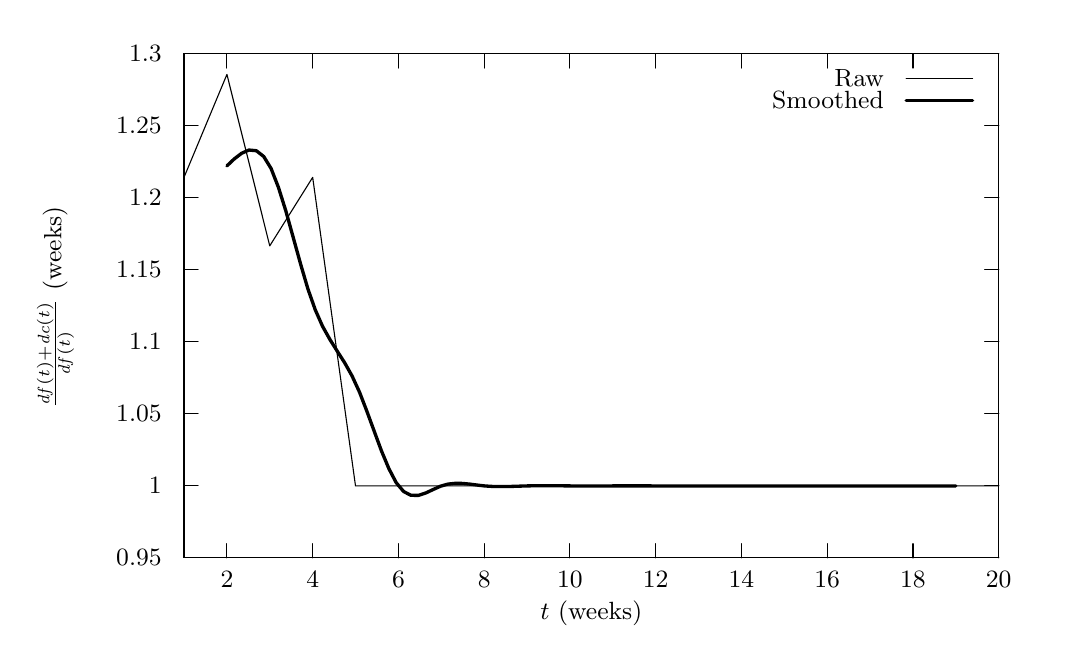
\begin{tikzpicture}[gnuplot]
%% generated with GNUPLOT 4.6p5 (Lua 5.2; terminal rev. 99, script rev. 100)
%% 2/09/2014 2:44:57 PM
\tikzset{every node/.append style={font={\fontsize{9pt}{10.8pt}\selectfont}}}
\gpmonochromelines
\path (0.000,0.000) rectangle (12.700,7.620);
\gpcolor{color=gp lt color border}
\gpsetlinetype{gp lt border}
\gpsetlinewidth{1.00}
\draw[gp path] (1.854,0.886)--(2.034,0.886);
\draw[gp path] (12.201,0.886)--(12.021,0.886);
\node[gp node right] at (1.688,0.886) { 0.95};
\draw[gp path] (1.854,1.800)--(2.034,1.800);
\draw[gp path] (12.201,1.800)--(12.021,1.800);
\node[gp node right] at (1.688,1.800) { 1};
\draw[gp path] (1.854,2.715)--(2.034,2.715);
\draw[gp path] (12.201,2.715)--(12.021,2.715);
\node[gp node right] at (1.688,2.715) { 1.05};
\draw[gp path] (1.854,3.629)--(2.034,3.629);
\draw[gp path] (12.201,3.629)--(12.021,3.629);
\node[gp node right] at (1.688,3.629) { 1.1};
\draw[gp path] (1.854,4.544)--(2.034,4.544);
\draw[gp path] (12.201,4.544)--(12.021,4.544);
\node[gp node right] at (1.688,4.544) { 1.15};
\draw[gp path] (1.854,5.458)--(2.034,5.458);
\draw[gp path] (12.201,5.458)--(12.021,5.458);
\node[gp node right] at (1.688,5.458) { 1.2};
\draw[gp path] (1.854,6.373)--(2.034,6.373);
\draw[gp path] (12.201,6.373)--(12.021,6.373);
\node[gp node right] at (1.688,6.373) { 1.25};
\draw[gp path] (1.854,7.287)--(2.034,7.287);
\draw[gp path] (12.201,7.287)--(12.021,7.287);
\node[gp node right] at (1.688,7.287) { 1.3};
\draw[gp path] (2.399,0.886)--(2.399,1.066);
\draw[gp path] (2.399,7.287)--(2.399,7.107);
\node[gp node center] at (2.399,0.609) { 2};
\draw[gp path] (3.488,0.886)--(3.488,1.066);
\draw[gp path] (3.488,7.287)--(3.488,7.107);
\node[gp node center] at (3.488,0.609) { 4};
\draw[gp path] (4.577,0.886)--(4.577,1.066);
\draw[gp path] (4.577,7.287)--(4.577,7.107);
\node[gp node center] at (4.577,0.609) { 6};
\draw[gp path] (5.666,0.886)--(5.666,1.066);
\draw[gp path] (5.666,7.287)--(5.666,7.107);
\node[gp node center] at (5.666,0.609) { 8};
\draw[gp path] (6.755,0.886)--(6.755,1.066);
\draw[gp path] (6.755,7.287)--(6.755,7.107);
\node[gp node center] at (6.755,0.609) { 10};
\draw[gp path] (7.844,0.886)--(7.844,1.066);
\draw[gp path] (7.844,7.287)--(7.844,7.107);
\node[gp node center] at (7.844,0.609) { 12};
\draw[gp path] (8.934,0.886)--(8.934,1.066);
\draw[gp path] (8.934,7.287)--(8.934,7.107);
\node[gp node center] at (8.934,0.609) { 14};
\draw[gp path] (10.023,0.886)--(10.023,1.066);
\draw[gp path] (10.023,7.287)--(10.023,7.107);
\node[gp node center] at (10.023,0.609) { 16};
\draw[gp path] (11.112,0.886)--(11.112,1.066);
\draw[gp path] (11.112,7.287)--(11.112,7.107);
\node[gp node center] at (11.112,0.609) { 18};
\draw[gp path] (12.201,0.886)--(12.201,1.066);
\draw[gp path] (12.201,7.287)--(12.201,7.107);
\node[gp node center] at (12.201,0.609) { 20};
\draw[gp path] (1.854,7.287)--(1.854,0.886)--(12.201,0.886)--(12.201,7.287)--cycle;
\node[gp node center,rotate=-270] at (0.221,4.086) {$\frac{\mathit{df}(t) + \mathit{dc}(t)}{\mathit{df}(t)}$ (weeks)};
\node[gp node center] at (7.027,0.194) {$t$ (weeks)};
\node[gp node right] at (10.859,6.969) {Raw};
\gpcolor{color=gp lt color 3}
\gpsetlinetype{gp lt plot 3}
\draw[gp path] (11.025,6.969)--(11.869,6.969);
\draw[gp path] (1.854,5.719)--(2.399,7.026)--(2.943,4.849)--(3.488,5.719)--(4.032,1.800)%
  --(4.577,1.800)--(5.121,1.800)--(5.666,1.800)--(6.211,1.800)--(6.755,1.800)--(7.300,1.800)%
  --(7.844,1.800)--(8.389,1.800)--(8.934,1.800)--(9.478,1.800)--(10.023,1.800)--(10.567,1.800)%
  --(11.656,1.800)--(12.201,1.800);
\gpcolor{color=gp lt color border}
\node[gp node right] at (10.859,6.692) {Smoothed};
\gpcolor{color=gp lt color 0}
\gpsetlinetype{gp lt plot 0}
\gpsetlinewidth{3.00}
\draw[gp path] (11.025,6.692)--(11.869,6.692);
\draw[gp path] (2.399,5.865)--(2.492,5.953)--(2.586,6.025)--(2.679,6.066)--(2.773,6.057)%
  --(2.866,5.984)--(2.960,5.831)--(3.053,5.592)--(3.147,5.293)--(3.240,4.959)--(3.334,4.620)%
  --(3.427,4.303)--(3.521,4.036)--(3.614,3.826)--(3.708,3.658)--(3.801,3.510)--(3.895,3.363)%
  --(3.988,3.197)--(4.082,2.993)--(4.175,2.752)--(4.269,2.496)--(4.362,2.244)--(4.456,2.019)%
  --(4.549,1.841)--(4.643,1.729)--(4.736,1.681)--(4.830,1.680)--(4.923,1.710)--(5.017,1.754)%
  --(5.110,1.796)--(5.204,1.823)--(5.297,1.833)--(5.391,1.832)--(5.485,1.823)--(5.578,1.811)%
  --(5.672,1.800)--(5.765,1.794)--(5.859,1.792)--(5.952,1.792)--(6.046,1.795)--(6.139,1.798)%
  --(6.233,1.801)--(6.326,1.802)--(6.420,1.803)--(6.513,1.802)--(6.607,1.802)--(6.700,1.801)%
  --(6.794,1.800)--(6.887,1.800)--(6.981,1.800)--(7.074,1.800)--(7.168,1.800)--(7.261,1.800)%
  --(7.355,1.801)--(7.448,1.801)--(7.542,1.801)--(7.635,1.801)--(7.729,1.801)--(7.822,1.800)%
  --(7.916,1.800)--(8.009,1.800)--(8.103,1.800)--(8.196,1.800)--(8.290,1.800)--(8.383,1.800)%
  --(8.477,1.800)--(8.570,1.800)--(8.664,1.800)--(8.758,1.800)--(8.851,1.800)--(8.945,1.800)%
  --(9.038,1.800)--(9.132,1.800)--(9.225,1.800)--(9.319,1.800)--(9.412,1.800)--(9.506,1.800)%
  --(9.599,1.800)--(9.693,1.800)--(9.786,1.800)--(9.880,1.800)--(9.973,1.800)--(10.067,1.800)%
  --(10.160,1.800)--(10.254,1.800)--(10.347,1.800)--(10.441,1.800)--(10.534,1.800)--(10.628,1.800)%
  --(10.721,1.800)--(10.815,1.800)--(10.908,1.800)--(11.002,1.800)--(11.095,1.800)--(11.189,1.800)%
  --(11.282,1.800)--(11.376,1.800)--(11.469,1.800)--(11.563,1.800)--(11.656,1.800);
\gpcolor{color=gp lt color border}
\gpsetlinetype{gp lt border}
\gpsetlinewidth{1.00}
\draw[gp path] (1.854,7.287)--(1.854,0.886)--(12.201,0.886)--(12.201,7.287)--cycle;
%% coordinates of the plot area
\gpdefrectangularnode{gp plot 1}{\pgfpoint{1.854cm}{0.886cm}}{\pgfpoint{12.201cm}{7.287cm}}
\end{tikzpicture}
%% gnuplot variables

    \caption{Easy--Hard, Major--Minor}
  \end{figure}
  
  \begin{figure}[!htb]
    \centering
    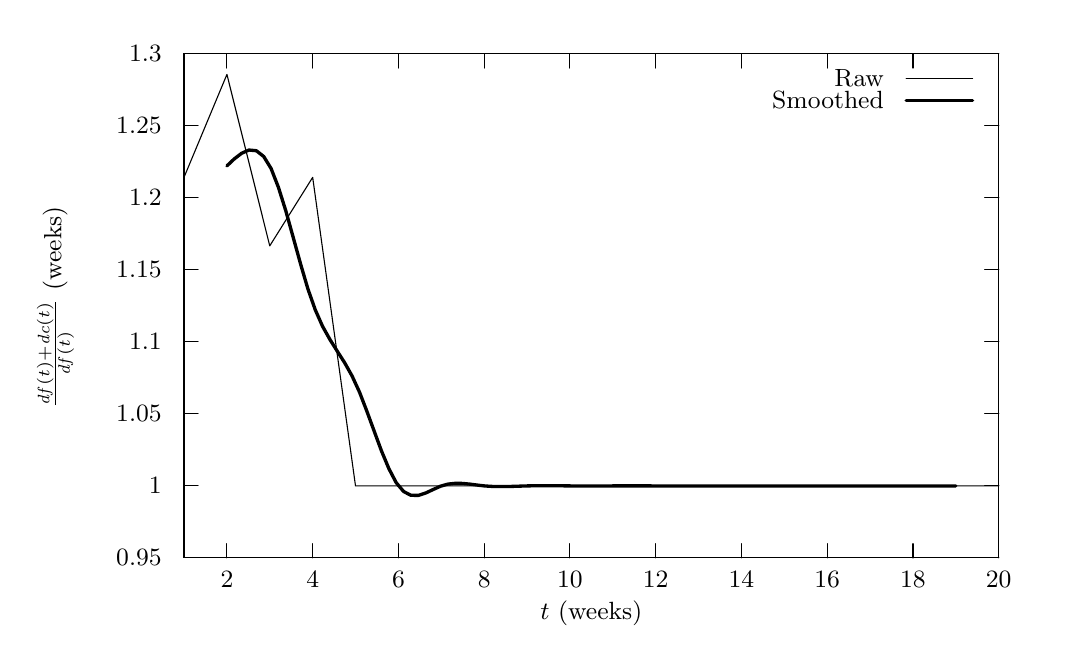
\begin{tikzpicture}[gnuplot]
%% generated with GNUPLOT 4.6p5 (Lua 5.2; terminal rev. 99, script rev. 100)
%% 2/09/2014 2:44:57 PM
\tikzset{every node/.append style={font={\fontsize{9pt}{10.8pt}\selectfont}}}
\gpmonochromelines
\path (0.000,0.000) rectangle (12.700,7.620);
\gpcolor{color=gp lt color border}
\gpsetlinetype{gp lt border}
\gpsetlinewidth{1.00}
\draw[gp path] (1.854,0.886)--(2.034,0.886);
\draw[gp path] (12.201,0.886)--(12.021,0.886);
\node[gp node right] at (1.688,0.886) { 0.95};
\draw[gp path] (1.854,1.800)--(2.034,1.800);
\draw[gp path] (12.201,1.800)--(12.021,1.800);
\node[gp node right] at (1.688,1.800) { 1};
\draw[gp path] (1.854,2.715)--(2.034,2.715);
\draw[gp path] (12.201,2.715)--(12.021,2.715);
\node[gp node right] at (1.688,2.715) { 1.05};
\draw[gp path] (1.854,3.629)--(2.034,3.629);
\draw[gp path] (12.201,3.629)--(12.021,3.629);
\node[gp node right] at (1.688,3.629) { 1.1};
\draw[gp path] (1.854,4.544)--(2.034,4.544);
\draw[gp path] (12.201,4.544)--(12.021,4.544);
\node[gp node right] at (1.688,4.544) { 1.15};
\draw[gp path] (1.854,5.458)--(2.034,5.458);
\draw[gp path] (12.201,5.458)--(12.021,5.458);
\node[gp node right] at (1.688,5.458) { 1.2};
\draw[gp path] (1.854,6.373)--(2.034,6.373);
\draw[gp path] (12.201,6.373)--(12.021,6.373);
\node[gp node right] at (1.688,6.373) { 1.25};
\draw[gp path] (1.854,7.287)--(2.034,7.287);
\draw[gp path] (12.201,7.287)--(12.021,7.287);
\node[gp node right] at (1.688,7.287) { 1.3};
\draw[gp path] (2.399,0.886)--(2.399,1.066);
\draw[gp path] (2.399,7.287)--(2.399,7.107);
\node[gp node center] at (2.399,0.609) { 2};
\draw[gp path] (3.488,0.886)--(3.488,1.066);
\draw[gp path] (3.488,7.287)--(3.488,7.107);
\node[gp node center] at (3.488,0.609) { 4};
\draw[gp path] (4.577,0.886)--(4.577,1.066);
\draw[gp path] (4.577,7.287)--(4.577,7.107);
\node[gp node center] at (4.577,0.609) { 6};
\draw[gp path] (5.666,0.886)--(5.666,1.066);
\draw[gp path] (5.666,7.287)--(5.666,7.107);
\node[gp node center] at (5.666,0.609) { 8};
\draw[gp path] (6.755,0.886)--(6.755,1.066);
\draw[gp path] (6.755,7.287)--(6.755,7.107);
\node[gp node center] at (6.755,0.609) { 10};
\draw[gp path] (7.844,0.886)--(7.844,1.066);
\draw[gp path] (7.844,7.287)--(7.844,7.107);
\node[gp node center] at (7.844,0.609) { 12};
\draw[gp path] (8.934,0.886)--(8.934,1.066);
\draw[gp path] (8.934,7.287)--(8.934,7.107);
\node[gp node center] at (8.934,0.609) { 14};
\draw[gp path] (10.023,0.886)--(10.023,1.066);
\draw[gp path] (10.023,7.287)--(10.023,7.107);
\node[gp node center] at (10.023,0.609) { 16};
\draw[gp path] (11.112,0.886)--(11.112,1.066);
\draw[gp path] (11.112,7.287)--(11.112,7.107);
\node[gp node center] at (11.112,0.609) { 18};
\draw[gp path] (12.201,0.886)--(12.201,1.066);
\draw[gp path] (12.201,7.287)--(12.201,7.107);
\node[gp node center] at (12.201,0.609) { 20};
\draw[gp path] (1.854,7.287)--(1.854,0.886)--(12.201,0.886)--(12.201,7.287)--cycle;
\node[gp node center,rotate=-270] at (0.221,4.086) {$\frac{\mathit{df}(t) + \mathit{dc}(t)}{\mathit{df}(t)}$ (weeks)};
\node[gp node center] at (7.027,0.194) {$t$ (weeks)};
\node[gp node right] at (10.859,6.969) {Raw};
\gpcolor{color=gp lt color 3}
\gpsetlinetype{gp lt plot 3}
\draw[gp path] (11.025,6.969)--(11.869,6.969);
\draw[gp path] (1.854,5.719)--(2.399,7.026)--(2.943,4.849)--(3.488,5.719)--(4.032,1.800)%
  --(4.577,1.800)--(5.121,1.800)--(5.666,1.800)--(6.211,1.800)--(6.755,1.800)--(7.300,1.800)%
  --(7.844,1.800)--(8.389,1.800)--(8.934,1.800)--(9.478,1.800)--(10.023,1.800)--(10.567,1.800)%
  --(11.656,1.800)--(12.201,1.800);
\gpcolor{color=gp lt color border}
\node[gp node right] at (10.859,6.692) {Smoothed};
\gpcolor{color=gp lt color 0}
\gpsetlinetype{gp lt plot 0}
\gpsetlinewidth{3.00}
\draw[gp path] (11.025,6.692)--(11.869,6.692);
\draw[gp path] (2.399,5.865)--(2.492,5.953)--(2.586,6.025)--(2.679,6.066)--(2.773,6.057)%
  --(2.866,5.984)--(2.960,5.831)--(3.053,5.592)--(3.147,5.293)--(3.240,4.959)--(3.334,4.620)%
  --(3.427,4.303)--(3.521,4.036)--(3.614,3.826)--(3.708,3.658)--(3.801,3.510)--(3.895,3.363)%
  --(3.988,3.197)--(4.082,2.993)--(4.175,2.752)--(4.269,2.496)--(4.362,2.244)--(4.456,2.019)%
  --(4.549,1.841)--(4.643,1.729)--(4.736,1.681)--(4.830,1.680)--(4.923,1.710)--(5.017,1.754)%
  --(5.110,1.796)--(5.204,1.823)--(5.297,1.833)--(5.391,1.832)--(5.485,1.823)--(5.578,1.811)%
  --(5.672,1.800)--(5.765,1.794)--(5.859,1.792)--(5.952,1.792)--(6.046,1.795)--(6.139,1.798)%
  --(6.233,1.801)--(6.326,1.802)--(6.420,1.803)--(6.513,1.802)--(6.607,1.802)--(6.700,1.801)%
  --(6.794,1.800)--(6.887,1.800)--(6.981,1.800)--(7.074,1.800)--(7.168,1.800)--(7.261,1.800)%
  --(7.355,1.801)--(7.448,1.801)--(7.542,1.801)--(7.635,1.801)--(7.729,1.801)--(7.822,1.800)%
  --(7.916,1.800)--(8.009,1.800)--(8.103,1.800)--(8.196,1.800)--(8.290,1.800)--(8.383,1.800)%
  --(8.477,1.800)--(8.570,1.800)--(8.664,1.800)--(8.758,1.800)--(8.851,1.800)--(8.945,1.800)%
  --(9.038,1.800)--(9.132,1.800)--(9.225,1.800)--(9.319,1.800)--(9.412,1.800)--(9.506,1.800)%
  --(9.599,1.800)--(9.693,1.800)--(9.786,1.800)--(9.880,1.800)--(9.973,1.800)--(10.067,1.800)%
  --(10.160,1.800)--(10.254,1.800)--(10.347,1.800)--(10.441,1.800)--(10.534,1.800)--(10.628,1.800)%
  --(10.721,1.800)--(10.815,1.800)--(10.908,1.800)--(11.002,1.800)--(11.095,1.800)--(11.189,1.800)%
  --(11.282,1.800)--(11.376,1.800)--(11.469,1.800)--(11.563,1.800)--(11.656,1.800);
\gpcolor{color=gp lt color border}
\gpsetlinetype{gp lt border}
\gpsetlinewidth{1.00}
\draw[gp path] (1.854,7.287)--(1.854,0.886)--(12.201,0.886)--(12.201,7.287)--cycle;
%% coordinates of the plot area
\gpdefrectangularnode{gp plot 1}{\pgfpoint{1.854cm}{0.886cm}}{\pgfpoint{12.201cm}{7.287cm}}
\end{tikzpicture}
%% gnuplot variables

    \caption{Hard--Easy, Major--Minor}
  \end{figure}
  
  \begin{figure}[!htb]
    \centering
    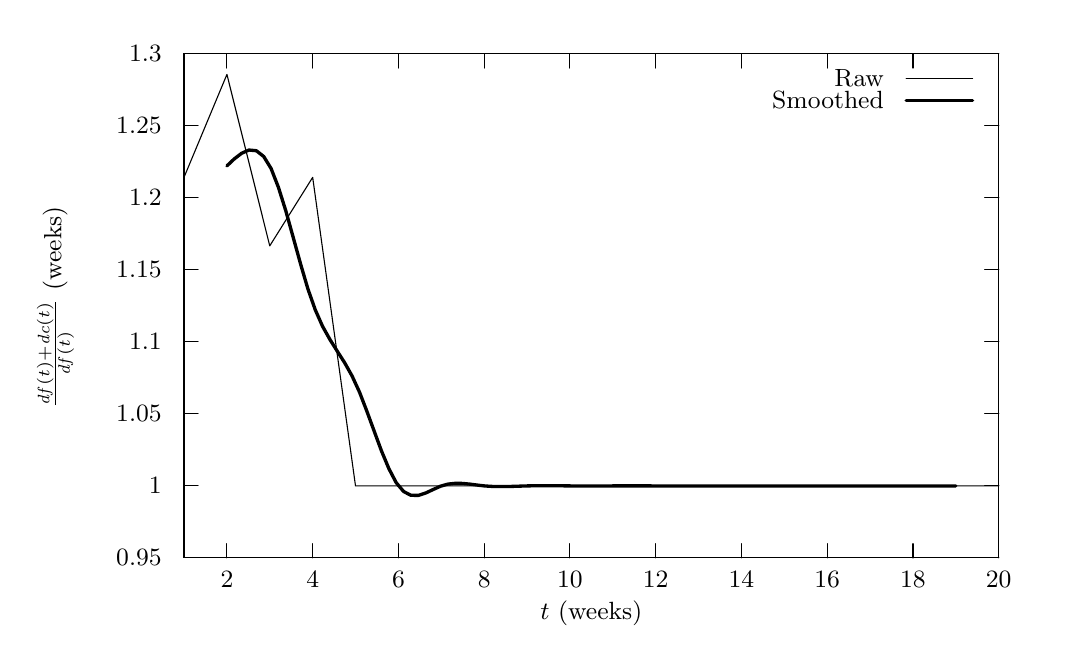
\begin{tikzpicture}[gnuplot]
%% generated with GNUPLOT 4.6p5 (Lua 5.2; terminal rev. 99, script rev. 100)
%% 2/09/2014 2:44:57 PM
\tikzset{every node/.append style={font={\fontsize{9pt}{10.8pt}\selectfont}}}
\gpmonochromelines
\path (0.000,0.000) rectangle (12.700,7.620);
\gpcolor{color=gp lt color border}
\gpsetlinetype{gp lt border}
\gpsetlinewidth{1.00}
\draw[gp path] (1.854,0.886)--(2.034,0.886);
\draw[gp path] (12.201,0.886)--(12.021,0.886);
\node[gp node right] at (1.688,0.886) { 0.95};
\draw[gp path] (1.854,1.800)--(2.034,1.800);
\draw[gp path] (12.201,1.800)--(12.021,1.800);
\node[gp node right] at (1.688,1.800) { 1};
\draw[gp path] (1.854,2.715)--(2.034,2.715);
\draw[gp path] (12.201,2.715)--(12.021,2.715);
\node[gp node right] at (1.688,2.715) { 1.05};
\draw[gp path] (1.854,3.629)--(2.034,3.629);
\draw[gp path] (12.201,3.629)--(12.021,3.629);
\node[gp node right] at (1.688,3.629) { 1.1};
\draw[gp path] (1.854,4.544)--(2.034,4.544);
\draw[gp path] (12.201,4.544)--(12.021,4.544);
\node[gp node right] at (1.688,4.544) { 1.15};
\draw[gp path] (1.854,5.458)--(2.034,5.458);
\draw[gp path] (12.201,5.458)--(12.021,5.458);
\node[gp node right] at (1.688,5.458) { 1.2};
\draw[gp path] (1.854,6.373)--(2.034,6.373);
\draw[gp path] (12.201,6.373)--(12.021,6.373);
\node[gp node right] at (1.688,6.373) { 1.25};
\draw[gp path] (1.854,7.287)--(2.034,7.287);
\draw[gp path] (12.201,7.287)--(12.021,7.287);
\node[gp node right] at (1.688,7.287) { 1.3};
\draw[gp path] (2.399,0.886)--(2.399,1.066);
\draw[gp path] (2.399,7.287)--(2.399,7.107);
\node[gp node center] at (2.399,0.609) { 2};
\draw[gp path] (3.488,0.886)--(3.488,1.066);
\draw[gp path] (3.488,7.287)--(3.488,7.107);
\node[gp node center] at (3.488,0.609) { 4};
\draw[gp path] (4.577,0.886)--(4.577,1.066);
\draw[gp path] (4.577,7.287)--(4.577,7.107);
\node[gp node center] at (4.577,0.609) { 6};
\draw[gp path] (5.666,0.886)--(5.666,1.066);
\draw[gp path] (5.666,7.287)--(5.666,7.107);
\node[gp node center] at (5.666,0.609) { 8};
\draw[gp path] (6.755,0.886)--(6.755,1.066);
\draw[gp path] (6.755,7.287)--(6.755,7.107);
\node[gp node center] at (6.755,0.609) { 10};
\draw[gp path] (7.844,0.886)--(7.844,1.066);
\draw[gp path] (7.844,7.287)--(7.844,7.107);
\node[gp node center] at (7.844,0.609) { 12};
\draw[gp path] (8.934,0.886)--(8.934,1.066);
\draw[gp path] (8.934,7.287)--(8.934,7.107);
\node[gp node center] at (8.934,0.609) { 14};
\draw[gp path] (10.023,0.886)--(10.023,1.066);
\draw[gp path] (10.023,7.287)--(10.023,7.107);
\node[gp node center] at (10.023,0.609) { 16};
\draw[gp path] (11.112,0.886)--(11.112,1.066);
\draw[gp path] (11.112,7.287)--(11.112,7.107);
\node[gp node center] at (11.112,0.609) { 18};
\draw[gp path] (12.201,0.886)--(12.201,1.066);
\draw[gp path] (12.201,7.287)--(12.201,7.107);
\node[gp node center] at (12.201,0.609) { 20};
\draw[gp path] (1.854,7.287)--(1.854,0.886)--(12.201,0.886)--(12.201,7.287)--cycle;
\node[gp node center,rotate=-270] at (0.221,4.086) {$\frac{\mathit{df}(t) + \mathit{dc}(t)}{\mathit{df}(t)}$ (weeks)};
\node[gp node center] at (7.027,0.194) {$t$ (weeks)};
\node[gp node right] at (10.859,6.969) {Raw};
\gpcolor{color=gp lt color 3}
\gpsetlinetype{gp lt plot 3}
\draw[gp path] (11.025,6.969)--(11.869,6.969);
\draw[gp path] (1.854,5.719)--(2.399,7.026)--(2.943,4.849)--(3.488,5.719)--(4.032,1.800)%
  --(4.577,1.800)--(5.121,1.800)--(5.666,1.800)--(6.211,1.800)--(6.755,1.800)--(7.300,1.800)%
  --(7.844,1.800)--(8.389,1.800)--(8.934,1.800)--(9.478,1.800)--(10.023,1.800)--(10.567,1.800)%
  --(11.656,1.800)--(12.201,1.800);
\gpcolor{color=gp lt color border}
\node[gp node right] at (10.859,6.692) {Smoothed};
\gpcolor{color=gp lt color 0}
\gpsetlinetype{gp lt plot 0}
\gpsetlinewidth{3.00}
\draw[gp path] (11.025,6.692)--(11.869,6.692);
\draw[gp path] (2.399,5.865)--(2.492,5.953)--(2.586,6.025)--(2.679,6.066)--(2.773,6.057)%
  --(2.866,5.984)--(2.960,5.831)--(3.053,5.592)--(3.147,5.293)--(3.240,4.959)--(3.334,4.620)%
  --(3.427,4.303)--(3.521,4.036)--(3.614,3.826)--(3.708,3.658)--(3.801,3.510)--(3.895,3.363)%
  --(3.988,3.197)--(4.082,2.993)--(4.175,2.752)--(4.269,2.496)--(4.362,2.244)--(4.456,2.019)%
  --(4.549,1.841)--(4.643,1.729)--(4.736,1.681)--(4.830,1.680)--(4.923,1.710)--(5.017,1.754)%
  --(5.110,1.796)--(5.204,1.823)--(5.297,1.833)--(5.391,1.832)--(5.485,1.823)--(5.578,1.811)%
  --(5.672,1.800)--(5.765,1.794)--(5.859,1.792)--(5.952,1.792)--(6.046,1.795)--(6.139,1.798)%
  --(6.233,1.801)--(6.326,1.802)--(6.420,1.803)--(6.513,1.802)--(6.607,1.802)--(6.700,1.801)%
  --(6.794,1.800)--(6.887,1.800)--(6.981,1.800)--(7.074,1.800)--(7.168,1.800)--(7.261,1.800)%
  --(7.355,1.801)--(7.448,1.801)--(7.542,1.801)--(7.635,1.801)--(7.729,1.801)--(7.822,1.800)%
  --(7.916,1.800)--(8.009,1.800)--(8.103,1.800)--(8.196,1.800)--(8.290,1.800)--(8.383,1.800)%
  --(8.477,1.800)--(8.570,1.800)--(8.664,1.800)--(8.758,1.800)--(8.851,1.800)--(8.945,1.800)%
  --(9.038,1.800)--(9.132,1.800)--(9.225,1.800)--(9.319,1.800)--(9.412,1.800)--(9.506,1.800)%
  --(9.599,1.800)--(9.693,1.800)--(9.786,1.800)--(9.880,1.800)--(9.973,1.800)--(10.067,1.800)%
  --(10.160,1.800)--(10.254,1.800)--(10.347,1.800)--(10.441,1.800)--(10.534,1.800)--(10.628,1.800)%
  --(10.721,1.800)--(10.815,1.800)--(10.908,1.800)--(11.002,1.800)--(11.095,1.800)--(11.189,1.800)%
  --(11.282,1.800)--(11.376,1.800)--(11.469,1.800)--(11.563,1.800)--(11.656,1.800);
\gpcolor{color=gp lt color border}
\gpsetlinetype{gp lt border}
\gpsetlinewidth{1.00}
\draw[gp path] (1.854,7.287)--(1.854,0.886)--(12.201,0.886)--(12.201,7.287)--cycle;
%% coordinates of the plot area
\gpdefrectangularnode{gp plot 1}{\pgfpoint{1.854cm}{0.886cm}}{\pgfpoint{12.201cm}{7.287cm}}
\end{tikzpicture}
%% gnuplot variables

    \caption{Major--Minor, Easy--Hard}
  \end{figure}
  
  \begin{figure}[!htb]
    \centering
    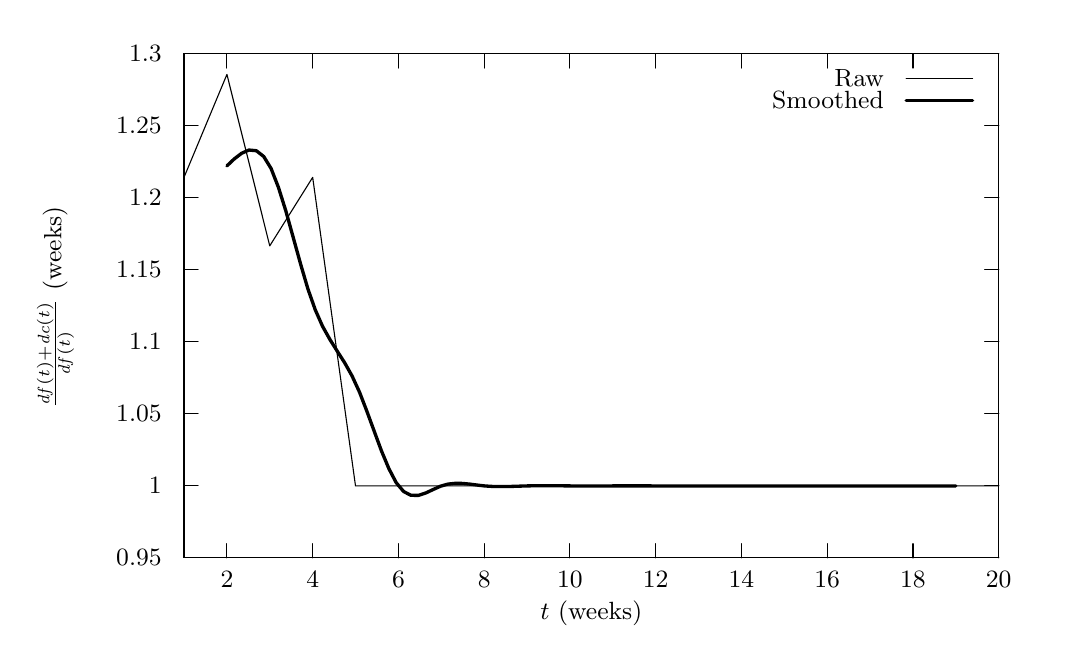
\begin{tikzpicture}[gnuplot]
%% generated with GNUPLOT 4.6p5 (Lua 5.2; terminal rev. 99, script rev. 100)
%% 2/09/2014 2:44:57 PM
\tikzset{every node/.append style={font={\fontsize{9pt}{10.8pt}\selectfont}}}
\gpmonochromelines
\path (0.000,0.000) rectangle (12.700,7.620);
\gpcolor{color=gp lt color border}
\gpsetlinetype{gp lt border}
\gpsetlinewidth{1.00}
\draw[gp path] (1.854,0.886)--(2.034,0.886);
\draw[gp path] (12.201,0.886)--(12.021,0.886);
\node[gp node right] at (1.688,0.886) { 0.95};
\draw[gp path] (1.854,1.800)--(2.034,1.800);
\draw[gp path] (12.201,1.800)--(12.021,1.800);
\node[gp node right] at (1.688,1.800) { 1};
\draw[gp path] (1.854,2.715)--(2.034,2.715);
\draw[gp path] (12.201,2.715)--(12.021,2.715);
\node[gp node right] at (1.688,2.715) { 1.05};
\draw[gp path] (1.854,3.629)--(2.034,3.629);
\draw[gp path] (12.201,3.629)--(12.021,3.629);
\node[gp node right] at (1.688,3.629) { 1.1};
\draw[gp path] (1.854,4.544)--(2.034,4.544);
\draw[gp path] (12.201,4.544)--(12.021,4.544);
\node[gp node right] at (1.688,4.544) { 1.15};
\draw[gp path] (1.854,5.458)--(2.034,5.458);
\draw[gp path] (12.201,5.458)--(12.021,5.458);
\node[gp node right] at (1.688,5.458) { 1.2};
\draw[gp path] (1.854,6.373)--(2.034,6.373);
\draw[gp path] (12.201,6.373)--(12.021,6.373);
\node[gp node right] at (1.688,6.373) { 1.25};
\draw[gp path] (1.854,7.287)--(2.034,7.287);
\draw[gp path] (12.201,7.287)--(12.021,7.287);
\node[gp node right] at (1.688,7.287) { 1.3};
\draw[gp path] (2.399,0.886)--(2.399,1.066);
\draw[gp path] (2.399,7.287)--(2.399,7.107);
\node[gp node center] at (2.399,0.609) { 2};
\draw[gp path] (3.488,0.886)--(3.488,1.066);
\draw[gp path] (3.488,7.287)--(3.488,7.107);
\node[gp node center] at (3.488,0.609) { 4};
\draw[gp path] (4.577,0.886)--(4.577,1.066);
\draw[gp path] (4.577,7.287)--(4.577,7.107);
\node[gp node center] at (4.577,0.609) { 6};
\draw[gp path] (5.666,0.886)--(5.666,1.066);
\draw[gp path] (5.666,7.287)--(5.666,7.107);
\node[gp node center] at (5.666,0.609) { 8};
\draw[gp path] (6.755,0.886)--(6.755,1.066);
\draw[gp path] (6.755,7.287)--(6.755,7.107);
\node[gp node center] at (6.755,0.609) { 10};
\draw[gp path] (7.844,0.886)--(7.844,1.066);
\draw[gp path] (7.844,7.287)--(7.844,7.107);
\node[gp node center] at (7.844,0.609) { 12};
\draw[gp path] (8.934,0.886)--(8.934,1.066);
\draw[gp path] (8.934,7.287)--(8.934,7.107);
\node[gp node center] at (8.934,0.609) { 14};
\draw[gp path] (10.023,0.886)--(10.023,1.066);
\draw[gp path] (10.023,7.287)--(10.023,7.107);
\node[gp node center] at (10.023,0.609) { 16};
\draw[gp path] (11.112,0.886)--(11.112,1.066);
\draw[gp path] (11.112,7.287)--(11.112,7.107);
\node[gp node center] at (11.112,0.609) { 18};
\draw[gp path] (12.201,0.886)--(12.201,1.066);
\draw[gp path] (12.201,7.287)--(12.201,7.107);
\node[gp node center] at (12.201,0.609) { 20};
\draw[gp path] (1.854,7.287)--(1.854,0.886)--(12.201,0.886)--(12.201,7.287)--cycle;
\node[gp node center,rotate=-270] at (0.221,4.086) {$\frac{\mathit{df}(t) + \mathit{dc}(t)}{\mathit{df}(t)}$ (weeks)};
\node[gp node center] at (7.027,0.194) {$t$ (weeks)};
\node[gp node right] at (10.859,6.969) {Raw};
\gpcolor{color=gp lt color 3}
\gpsetlinetype{gp lt plot 3}
\draw[gp path] (11.025,6.969)--(11.869,6.969);
\draw[gp path] (1.854,5.719)--(2.399,7.026)--(2.943,4.849)--(3.488,5.719)--(4.032,1.800)%
  --(4.577,1.800)--(5.121,1.800)--(5.666,1.800)--(6.211,1.800)--(6.755,1.800)--(7.300,1.800)%
  --(7.844,1.800)--(8.389,1.800)--(8.934,1.800)--(9.478,1.800)--(10.023,1.800)--(10.567,1.800)%
  --(11.656,1.800)--(12.201,1.800);
\gpcolor{color=gp lt color border}
\node[gp node right] at (10.859,6.692) {Smoothed};
\gpcolor{color=gp lt color 0}
\gpsetlinetype{gp lt plot 0}
\gpsetlinewidth{3.00}
\draw[gp path] (11.025,6.692)--(11.869,6.692);
\draw[gp path] (2.399,5.865)--(2.492,5.953)--(2.586,6.025)--(2.679,6.066)--(2.773,6.057)%
  --(2.866,5.984)--(2.960,5.831)--(3.053,5.592)--(3.147,5.293)--(3.240,4.959)--(3.334,4.620)%
  --(3.427,4.303)--(3.521,4.036)--(3.614,3.826)--(3.708,3.658)--(3.801,3.510)--(3.895,3.363)%
  --(3.988,3.197)--(4.082,2.993)--(4.175,2.752)--(4.269,2.496)--(4.362,2.244)--(4.456,2.019)%
  --(4.549,1.841)--(4.643,1.729)--(4.736,1.681)--(4.830,1.680)--(4.923,1.710)--(5.017,1.754)%
  --(5.110,1.796)--(5.204,1.823)--(5.297,1.833)--(5.391,1.832)--(5.485,1.823)--(5.578,1.811)%
  --(5.672,1.800)--(5.765,1.794)--(5.859,1.792)--(5.952,1.792)--(6.046,1.795)--(6.139,1.798)%
  --(6.233,1.801)--(6.326,1.802)--(6.420,1.803)--(6.513,1.802)--(6.607,1.802)--(6.700,1.801)%
  --(6.794,1.800)--(6.887,1.800)--(6.981,1.800)--(7.074,1.800)--(7.168,1.800)--(7.261,1.800)%
  --(7.355,1.801)--(7.448,1.801)--(7.542,1.801)--(7.635,1.801)--(7.729,1.801)--(7.822,1.800)%
  --(7.916,1.800)--(8.009,1.800)--(8.103,1.800)--(8.196,1.800)--(8.290,1.800)--(8.383,1.800)%
  --(8.477,1.800)--(8.570,1.800)--(8.664,1.800)--(8.758,1.800)--(8.851,1.800)--(8.945,1.800)%
  --(9.038,1.800)--(9.132,1.800)--(9.225,1.800)--(9.319,1.800)--(9.412,1.800)--(9.506,1.800)%
  --(9.599,1.800)--(9.693,1.800)--(9.786,1.800)--(9.880,1.800)--(9.973,1.800)--(10.067,1.800)%
  --(10.160,1.800)--(10.254,1.800)--(10.347,1.800)--(10.441,1.800)--(10.534,1.800)--(10.628,1.800)%
  --(10.721,1.800)--(10.815,1.800)--(10.908,1.800)--(11.002,1.800)--(11.095,1.800)--(11.189,1.800)%
  --(11.282,1.800)--(11.376,1.800)--(11.469,1.800)--(11.563,1.800)--(11.656,1.800);
\gpcolor{color=gp lt color border}
\gpsetlinetype{gp lt border}
\gpsetlinewidth{1.00}
\draw[gp path] (1.854,7.287)--(1.854,0.886)--(12.201,0.886)--(12.201,7.287)--cycle;
%% coordinates of the plot area
\gpdefrectangularnode{gp plot 1}{\pgfpoint{1.854cm}{0.886cm}}{\pgfpoint{12.201cm}{7.287cm}}
\end{tikzpicture}
%% gnuplot variables

    \caption{Minor--Major, Easy--Hard}
  \end{figure}
  
  \begin{figure}[!htb]
    \centering
    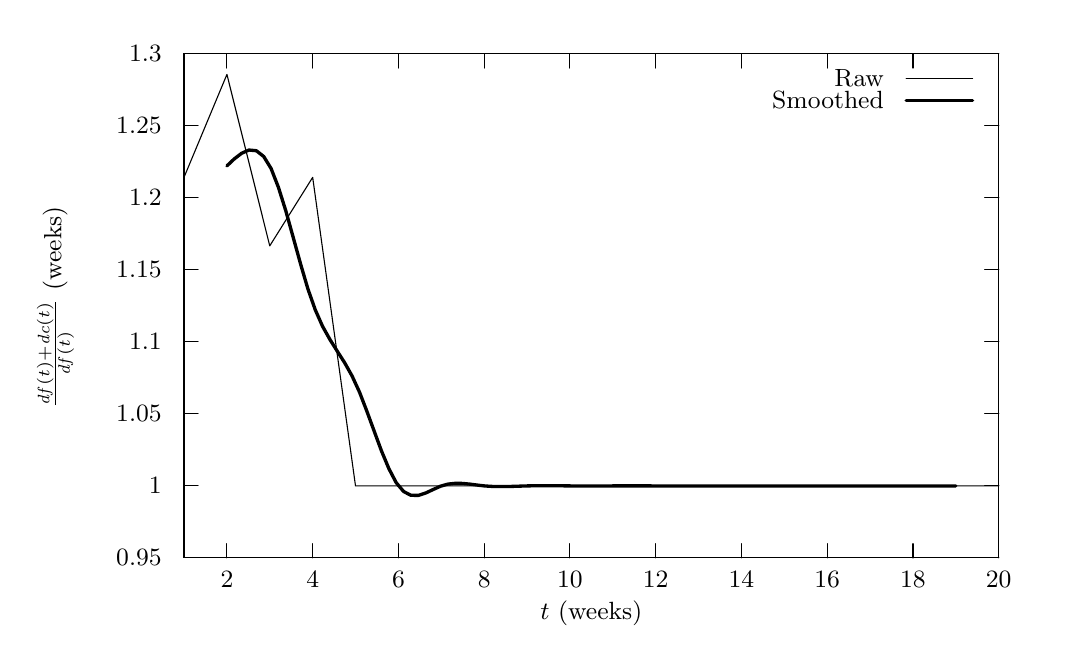
\begin{tikzpicture}[gnuplot]
%% generated with GNUPLOT 4.6p5 (Lua 5.2; terminal rev. 99, script rev. 100)
%% 2/09/2014 2:44:57 PM
\tikzset{every node/.append style={font={\fontsize{9pt}{10.8pt}\selectfont}}}
\gpmonochromelines
\path (0.000,0.000) rectangle (12.700,7.620);
\gpcolor{color=gp lt color border}
\gpsetlinetype{gp lt border}
\gpsetlinewidth{1.00}
\draw[gp path] (1.854,0.886)--(2.034,0.886);
\draw[gp path] (12.201,0.886)--(12.021,0.886);
\node[gp node right] at (1.688,0.886) { 0.95};
\draw[gp path] (1.854,1.800)--(2.034,1.800);
\draw[gp path] (12.201,1.800)--(12.021,1.800);
\node[gp node right] at (1.688,1.800) { 1};
\draw[gp path] (1.854,2.715)--(2.034,2.715);
\draw[gp path] (12.201,2.715)--(12.021,2.715);
\node[gp node right] at (1.688,2.715) { 1.05};
\draw[gp path] (1.854,3.629)--(2.034,3.629);
\draw[gp path] (12.201,3.629)--(12.021,3.629);
\node[gp node right] at (1.688,3.629) { 1.1};
\draw[gp path] (1.854,4.544)--(2.034,4.544);
\draw[gp path] (12.201,4.544)--(12.021,4.544);
\node[gp node right] at (1.688,4.544) { 1.15};
\draw[gp path] (1.854,5.458)--(2.034,5.458);
\draw[gp path] (12.201,5.458)--(12.021,5.458);
\node[gp node right] at (1.688,5.458) { 1.2};
\draw[gp path] (1.854,6.373)--(2.034,6.373);
\draw[gp path] (12.201,6.373)--(12.021,6.373);
\node[gp node right] at (1.688,6.373) { 1.25};
\draw[gp path] (1.854,7.287)--(2.034,7.287);
\draw[gp path] (12.201,7.287)--(12.021,7.287);
\node[gp node right] at (1.688,7.287) { 1.3};
\draw[gp path] (2.399,0.886)--(2.399,1.066);
\draw[gp path] (2.399,7.287)--(2.399,7.107);
\node[gp node center] at (2.399,0.609) { 2};
\draw[gp path] (3.488,0.886)--(3.488,1.066);
\draw[gp path] (3.488,7.287)--(3.488,7.107);
\node[gp node center] at (3.488,0.609) { 4};
\draw[gp path] (4.577,0.886)--(4.577,1.066);
\draw[gp path] (4.577,7.287)--(4.577,7.107);
\node[gp node center] at (4.577,0.609) { 6};
\draw[gp path] (5.666,0.886)--(5.666,1.066);
\draw[gp path] (5.666,7.287)--(5.666,7.107);
\node[gp node center] at (5.666,0.609) { 8};
\draw[gp path] (6.755,0.886)--(6.755,1.066);
\draw[gp path] (6.755,7.287)--(6.755,7.107);
\node[gp node center] at (6.755,0.609) { 10};
\draw[gp path] (7.844,0.886)--(7.844,1.066);
\draw[gp path] (7.844,7.287)--(7.844,7.107);
\node[gp node center] at (7.844,0.609) { 12};
\draw[gp path] (8.934,0.886)--(8.934,1.066);
\draw[gp path] (8.934,7.287)--(8.934,7.107);
\node[gp node center] at (8.934,0.609) { 14};
\draw[gp path] (10.023,0.886)--(10.023,1.066);
\draw[gp path] (10.023,7.287)--(10.023,7.107);
\node[gp node center] at (10.023,0.609) { 16};
\draw[gp path] (11.112,0.886)--(11.112,1.066);
\draw[gp path] (11.112,7.287)--(11.112,7.107);
\node[gp node center] at (11.112,0.609) { 18};
\draw[gp path] (12.201,0.886)--(12.201,1.066);
\draw[gp path] (12.201,7.287)--(12.201,7.107);
\node[gp node center] at (12.201,0.609) { 20};
\draw[gp path] (1.854,7.287)--(1.854,0.886)--(12.201,0.886)--(12.201,7.287)--cycle;
\node[gp node center,rotate=-270] at (0.221,4.086) {$\frac{\mathit{df}(t) + \mathit{dc}(t)}{\mathit{df}(t)}$ (weeks)};
\node[gp node center] at (7.027,0.194) {$t$ (weeks)};
\node[gp node right] at (10.859,6.969) {Raw};
\gpcolor{color=gp lt color 3}
\gpsetlinetype{gp lt plot 3}
\draw[gp path] (11.025,6.969)--(11.869,6.969);
\draw[gp path] (1.854,5.719)--(2.399,7.026)--(2.943,4.849)--(3.488,5.719)--(4.032,1.800)%
  --(4.577,1.800)--(5.121,1.800)--(5.666,1.800)--(6.211,1.800)--(6.755,1.800)--(7.300,1.800)%
  --(7.844,1.800)--(8.389,1.800)--(8.934,1.800)--(9.478,1.800)--(10.023,1.800)--(10.567,1.800)%
  --(11.656,1.800)--(12.201,1.800);
\gpcolor{color=gp lt color border}
\node[gp node right] at (10.859,6.692) {Smoothed};
\gpcolor{color=gp lt color 0}
\gpsetlinetype{gp lt plot 0}
\gpsetlinewidth{3.00}
\draw[gp path] (11.025,6.692)--(11.869,6.692);
\draw[gp path] (2.399,5.865)--(2.492,5.953)--(2.586,6.025)--(2.679,6.066)--(2.773,6.057)%
  --(2.866,5.984)--(2.960,5.831)--(3.053,5.592)--(3.147,5.293)--(3.240,4.959)--(3.334,4.620)%
  --(3.427,4.303)--(3.521,4.036)--(3.614,3.826)--(3.708,3.658)--(3.801,3.510)--(3.895,3.363)%
  --(3.988,3.197)--(4.082,2.993)--(4.175,2.752)--(4.269,2.496)--(4.362,2.244)--(4.456,2.019)%
  --(4.549,1.841)--(4.643,1.729)--(4.736,1.681)--(4.830,1.680)--(4.923,1.710)--(5.017,1.754)%
  --(5.110,1.796)--(5.204,1.823)--(5.297,1.833)--(5.391,1.832)--(5.485,1.823)--(5.578,1.811)%
  --(5.672,1.800)--(5.765,1.794)--(5.859,1.792)--(5.952,1.792)--(6.046,1.795)--(6.139,1.798)%
  --(6.233,1.801)--(6.326,1.802)--(6.420,1.803)--(6.513,1.802)--(6.607,1.802)--(6.700,1.801)%
  --(6.794,1.800)--(6.887,1.800)--(6.981,1.800)--(7.074,1.800)--(7.168,1.800)--(7.261,1.800)%
  --(7.355,1.801)--(7.448,1.801)--(7.542,1.801)--(7.635,1.801)--(7.729,1.801)--(7.822,1.800)%
  --(7.916,1.800)--(8.009,1.800)--(8.103,1.800)--(8.196,1.800)--(8.290,1.800)--(8.383,1.800)%
  --(8.477,1.800)--(8.570,1.800)--(8.664,1.800)--(8.758,1.800)--(8.851,1.800)--(8.945,1.800)%
  --(9.038,1.800)--(9.132,1.800)--(9.225,1.800)--(9.319,1.800)--(9.412,1.800)--(9.506,1.800)%
  --(9.599,1.800)--(9.693,1.800)--(9.786,1.800)--(9.880,1.800)--(9.973,1.800)--(10.067,1.800)%
  --(10.160,1.800)--(10.254,1.800)--(10.347,1.800)--(10.441,1.800)--(10.534,1.800)--(10.628,1.800)%
  --(10.721,1.800)--(10.815,1.800)--(10.908,1.800)--(11.002,1.800)--(11.095,1.800)--(11.189,1.800)%
  --(11.282,1.800)--(11.376,1.800)--(11.469,1.800)--(11.563,1.800)--(11.656,1.800);
\gpcolor{color=gp lt color border}
\gpsetlinetype{gp lt border}
\gpsetlinewidth{1.00}
\draw[gp path] (1.854,7.287)--(1.854,0.886)--(12.201,0.886)--(12.201,7.287)--cycle;
%% coordinates of the plot area
\gpdefrectangularnode{gp plot 1}{\pgfpoint{1.854cm}{0.886cm}}{\pgfpoint{12.201cm}{7.287cm}}
\end{tikzpicture}
%% gnuplot variables

    \caption{Random}
  \end{figure}
  
  \begin{figure}[!htb]
    \centering
    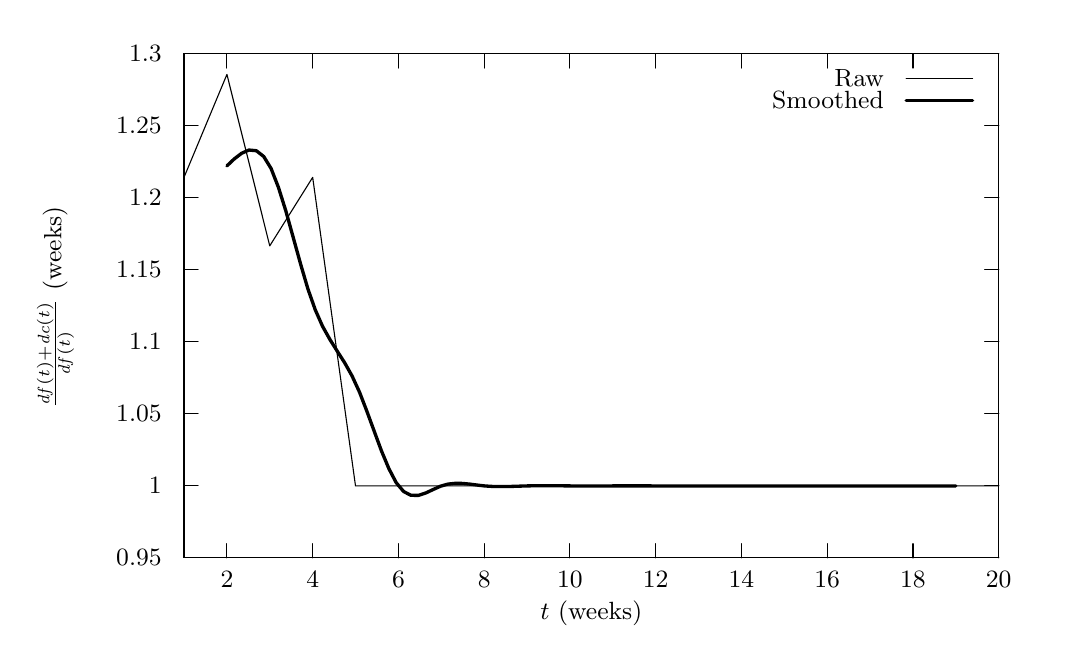
\begin{tikzpicture}[gnuplot]
%% generated with GNUPLOT 4.6p5 (Lua 5.2; terminal rev. 99, script rev. 100)
%% 2/09/2014 2:44:57 PM
\tikzset{every node/.append style={font={\fontsize{9pt}{10.8pt}\selectfont}}}
\gpmonochromelines
\path (0.000,0.000) rectangle (12.700,7.620);
\gpcolor{color=gp lt color border}
\gpsetlinetype{gp lt border}
\gpsetlinewidth{1.00}
\draw[gp path] (1.854,0.886)--(2.034,0.886);
\draw[gp path] (12.201,0.886)--(12.021,0.886);
\node[gp node right] at (1.688,0.886) { 0.95};
\draw[gp path] (1.854,1.800)--(2.034,1.800);
\draw[gp path] (12.201,1.800)--(12.021,1.800);
\node[gp node right] at (1.688,1.800) { 1};
\draw[gp path] (1.854,2.715)--(2.034,2.715);
\draw[gp path] (12.201,2.715)--(12.021,2.715);
\node[gp node right] at (1.688,2.715) { 1.05};
\draw[gp path] (1.854,3.629)--(2.034,3.629);
\draw[gp path] (12.201,3.629)--(12.021,3.629);
\node[gp node right] at (1.688,3.629) { 1.1};
\draw[gp path] (1.854,4.544)--(2.034,4.544);
\draw[gp path] (12.201,4.544)--(12.021,4.544);
\node[gp node right] at (1.688,4.544) { 1.15};
\draw[gp path] (1.854,5.458)--(2.034,5.458);
\draw[gp path] (12.201,5.458)--(12.021,5.458);
\node[gp node right] at (1.688,5.458) { 1.2};
\draw[gp path] (1.854,6.373)--(2.034,6.373);
\draw[gp path] (12.201,6.373)--(12.021,6.373);
\node[gp node right] at (1.688,6.373) { 1.25};
\draw[gp path] (1.854,7.287)--(2.034,7.287);
\draw[gp path] (12.201,7.287)--(12.021,7.287);
\node[gp node right] at (1.688,7.287) { 1.3};
\draw[gp path] (2.399,0.886)--(2.399,1.066);
\draw[gp path] (2.399,7.287)--(2.399,7.107);
\node[gp node center] at (2.399,0.609) { 2};
\draw[gp path] (3.488,0.886)--(3.488,1.066);
\draw[gp path] (3.488,7.287)--(3.488,7.107);
\node[gp node center] at (3.488,0.609) { 4};
\draw[gp path] (4.577,0.886)--(4.577,1.066);
\draw[gp path] (4.577,7.287)--(4.577,7.107);
\node[gp node center] at (4.577,0.609) { 6};
\draw[gp path] (5.666,0.886)--(5.666,1.066);
\draw[gp path] (5.666,7.287)--(5.666,7.107);
\node[gp node center] at (5.666,0.609) { 8};
\draw[gp path] (6.755,0.886)--(6.755,1.066);
\draw[gp path] (6.755,7.287)--(6.755,7.107);
\node[gp node center] at (6.755,0.609) { 10};
\draw[gp path] (7.844,0.886)--(7.844,1.066);
\draw[gp path] (7.844,7.287)--(7.844,7.107);
\node[gp node center] at (7.844,0.609) { 12};
\draw[gp path] (8.934,0.886)--(8.934,1.066);
\draw[gp path] (8.934,7.287)--(8.934,7.107);
\node[gp node center] at (8.934,0.609) { 14};
\draw[gp path] (10.023,0.886)--(10.023,1.066);
\draw[gp path] (10.023,7.287)--(10.023,7.107);
\node[gp node center] at (10.023,0.609) { 16};
\draw[gp path] (11.112,0.886)--(11.112,1.066);
\draw[gp path] (11.112,7.287)--(11.112,7.107);
\node[gp node center] at (11.112,0.609) { 18};
\draw[gp path] (12.201,0.886)--(12.201,1.066);
\draw[gp path] (12.201,7.287)--(12.201,7.107);
\node[gp node center] at (12.201,0.609) { 20};
\draw[gp path] (1.854,7.287)--(1.854,0.886)--(12.201,0.886)--(12.201,7.287)--cycle;
\node[gp node center,rotate=-270] at (0.221,4.086) {$\frac{\mathit{df}(t) + \mathit{dc}(t)}{\mathit{df}(t)}$ (weeks)};
\node[gp node center] at (7.027,0.194) {$t$ (weeks)};
\node[gp node right] at (10.859,6.969) {Raw};
\gpcolor{color=gp lt color 3}
\gpsetlinetype{gp lt plot 3}
\draw[gp path] (11.025,6.969)--(11.869,6.969);
\draw[gp path] (1.854,5.719)--(2.399,7.026)--(2.943,4.849)--(3.488,5.719)--(4.032,1.800)%
  --(4.577,1.800)--(5.121,1.800)--(5.666,1.800)--(6.211,1.800)--(6.755,1.800)--(7.300,1.800)%
  --(7.844,1.800)--(8.389,1.800)--(8.934,1.800)--(9.478,1.800)--(10.023,1.800)--(10.567,1.800)%
  --(11.656,1.800)--(12.201,1.800);
\gpcolor{color=gp lt color border}
\node[gp node right] at (10.859,6.692) {Smoothed};
\gpcolor{color=gp lt color 0}
\gpsetlinetype{gp lt plot 0}
\gpsetlinewidth{3.00}
\draw[gp path] (11.025,6.692)--(11.869,6.692);
\draw[gp path] (2.399,5.865)--(2.492,5.953)--(2.586,6.025)--(2.679,6.066)--(2.773,6.057)%
  --(2.866,5.984)--(2.960,5.831)--(3.053,5.592)--(3.147,5.293)--(3.240,4.959)--(3.334,4.620)%
  --(3.427,4.303)--(3.521,4.036)--(3.614,3.826)--(3.708,3.658)--(3.801,3.510)--(3.895,3.363)%
  --(3.988,3.197)--(4.082,2.993)--(4.175,2.752)--(4.269,2.496)--(4.362,2.244)--(4.456,2.019)%
  --(4.549,1.841)--(4.643,1.729)--(4.736,1.681)--(4.830,1.680)--(4.923,1.710)--(5.017,1.754)%
  --(5.110,1.796)--(5.204,1.823)--(5.297,1.833)--(5.391,1.832)--(5.485,1.823)--(5.578,1.811)%
  --(5.672,1.800)--(5.765,1.794)--(5.859,1.792)--(5.952,1.792)--(6.046,1.795)--(6.139,1.798)%
  --(6.233,1.801)--(6.326,1.802)--(6.420,1.803)--(6.513,1.802)--(6.607,1.802)--(6.700,1.801)%
  --(6.794,1.800)--(6.887,1.800)--(6.981,1.800)--(7.074,1.800)--(7.168,1.800)--(7.261,1.800)%
  --(7.355,1.801)--(7.448,1.801)--(7.542,1.801)--(7.635,1.801)--(7.729,1.801)--(7.822,1.800)%
  --(7.916,1.800)--(8.009,1.800)--(8.103,1.800)--(8.196,1.800)--(8.290,1.800)--(8.383,1.800)%
  --(8.477,1.800)--(8.570,1.800)--(8.664,1.800)--(8.758,1.800)--(8.851,1.800)--(8.945,1.800)%
  --(9.038,1.800)--(9.132,1.800)--(9.225,1.800)--(9.319,1.800)--(9.412,1.800)--(9.506,1.800)%
  --(9.599,1.800)--(9.693,1.800)--(9.786,1.800)--(9.880,1.800)--(9.973,1.800)--(10.067,1.800)%
  --(10.160,1.800)--(10.254,1.800)--(10.347,1.800)--(10.441,1.800)--(10.534,1.800)--(10.628,1.800)%
  --(10.721,1.800)--(10.815,1.800)--(10.908,1.800)--(11.002,1.800)--(11.095,1.800)--(11.189,1.800)%
  --(11.282,1.800)--(11.376,1.800)--(11.469,1.800)--(11.563,1.800)--(11.656,1.800);
\gpcolor{color=gp lt color border}
\gpsetlinetype{gp lt border}
\gpsetlinewidth{1.00}
\draw[gp path] (1.854,7.287)--(1.854,0.886)--(12.201,0.886)--(12.201,7.287)--cycle;
%% coordinates of the plot area
\gpdefrectangularnode{gp plot 1}{\pgfpoint{1.854cm}{0.886cm}}{\pgfpoint{12.201cm}{7.287cm}}
\end{tikzpicture}
%% gnuplot variables

    \caption{First In, First Out}
  \end{figure}
  
%  \begin{table}[!htb]
%    \centering
%    \csvreader[no head,tabular=|r|r|r|r|r|r|r|,
%	table head=\hline Week & EH MaMi & HE MaMi & MaMi EH & MiMa EH & Random & FIFO\\\hline\hline,
%	late after line=\\\hline]%
%      {dexport/aggregate/queuetime-round.csv}{1=\week,2=\ehmami,3=\fifo,4=\hemami,5=\mamieh,6=\mimaeh,7=\randomr}%
%      {\week & \ehmami & \hemami & \mamieh & \mimaeh & \randomr & \fifo}%
%    \caption{Data}
%  \end{table}
  
  \clearpage
  \subsection{Estimate of number of unfixed defects still in software}
  \begin{figure}[!htb]
    \centering
    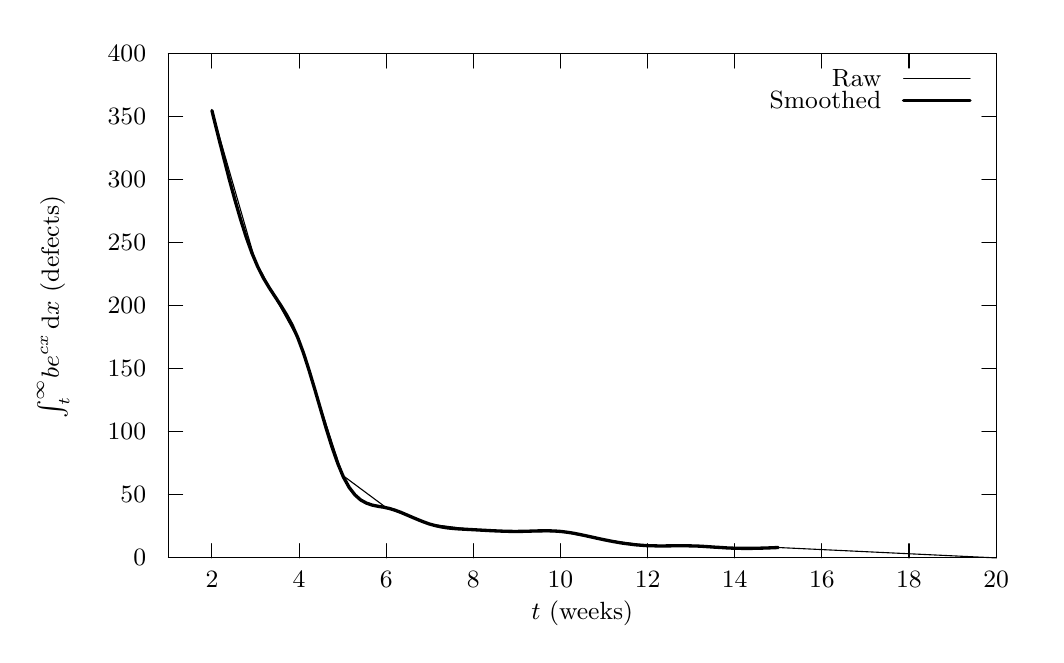
\begin{tikzpicture}[gnuplot]
%% generated with GNUPLOT 4.6p4 (Lua 5.1; terminal rev. 99, script rev. 100)
%% Thu 04 Sep 2014 10:50:27 WST
\tikzset{every node/.append style={font={\fontsize{9pt}{10.8pt}\selectfont}}}
\gpmonochromelines
\path (0.000,0.000) rectangle (12.700,7.620);
\gpcolor{color=gp lt color border}
\gpsetlinetype{gp lt border}
\gpsetlinewidth{1.00}
\draw[gp path] (1.688,0.886)--(1.868,0.886);
\draw[gp path] (12.201,0.886)--(12.021,0.886);
\node[gp node right] at (1.522,0.886) { 0};
\draw[gp path] (1.688,1.686)--(1.868,1.686);
\draw[gp path] (12.201,1.686)--(12.021,1.686);
\node[gp node right] at (1.522,1.686) { 50};
\draw[gp path] (1.688,2.486)--(1.868,2.486);
\draw[gp path] (12.201,2.486)--(12.021,2.486);
\node[gp node right] at (1.522,2.486) { 100};
\draw[gp path] (1.688,3.286)--(1.868,3.286);
\draw[gp path] (12.201,3.286)--(12.021,3.286);
\node[gp node right] at (1.522,3.286) { 150};
\draw[gp path] (1.688,4.087)--(1.868,4.087);
\draw[gp path] (12.201,4.087)--(12.021,4.087);
\node[gp node right] at (1.522,4.087) { 200};
\draw[gp path] (1.688,4.887)--(1.868,4.887);
\draw[gp path] (12.201,4.887)--(12.021,4.887);
\node[gp node right] at (1.522,4.887) { 250};
\draw[gp path] (1.688,5.687)--(1.868,5.687);
\draw[gp path] (12.201,5.687)--(12.021,5.687);
\node[gp node right] at (1.522,5.687) { 300};
\draw[gp path] (1.688,6.487)--(1.868,6.487);
\draw[gp path] (12.201,6.487)--(12.021,6.487);
\node[gp node right] at (1.522,6.487) { 350};
\draw[gp path] (1.688,7.287)--(1.868,7.287);
\draw[gp path] (12.201,7.287)--(12.021,7.287);
\node[gp node right] at (1.522,7.287) { 400};
\draw[gp path] (2.241,0.886)--(2.241,1.066);
\draw[gp path] (2.241,7.287)--(2.241,7.107);
\node[gp node center] at (2.241,0.609) { 2};
\draw[gp path] (3.348,0.886)--(3.348,1.066);
\draw[gp path] (3.348,7.287)--(3.348,7.107);
\node[gp node center] at (3.348,0.609) { 4};
\draw[gp path] (4.455,0.886)--(4.455,1.066);
\draw[gp path] (4.455,7.287)--(4.455,7.107);
\node[gp node center] at (4.455,0.609) { 6};
\draw[gp path] (5.561,0.886)--(5.561,1.066);
\draw[gp path] (5.561,7.287)--(5.561,7.107);
\node[gp node center] at (5.561,0.609) { 8};
\draw[gp path] (6.668,0.886)--(6.668,1.066);
\draw[gp path] (6.668,7.287)--(6.668,7.107);
\node[gp node center] at (6.668,0.609) { 10};
\draw[gp path] (7.774,0.886)--(7.774,1.066);
\draw[gp path] (7.774,7.287)--(7.774,7.107);
\node[gp node center] at (7.774,0.609) { 12};
\draw[gp path] (8.881,0.886)--(8.881,1.066);
\draw[gp path] (8.881,7.287)--(8.881,7.107);
\node[gp node center] at (8.881,0.609) { 14};
\draw[gp path] (9.988,0.886)--(9.988,1.066);
\draw[gp path] (9.988,7.287)--(9.988,7.107);
\node[gp node center] at (9.988,0.609) { 16};
\draw[gp path] (11.094,0.886)--(11.094,1.066);
\draw[gp path] (11.094,7.287)--(11.094,7.107);
\node[gp node center] at (11.094,0.609) { 18};
\draw[gp path] (12.201,0.886)--(12.201,1.066);
\draw[gp path] (12.201,7.287)--(12.201,7.107);
\node[gp node center] at (12.201,0.609) { 20};
\draw[gp path] (1.688,7.287)--(1.688,0.886)--(12.201,0.886)--(12.201,7.287)--cycle;
\node[gp node center,rotate=-270] at (0.221,4.086) {$\int_{t}^{\infty} \! be^{cx} \, \mathrm{d}x$ (defects)};
\node[gp node center] at (6.944,0.194) {$t$ (weeks)};
\node[gp node right] at (10.859,6.969) {Raw};
\gpcolor{color=gp lt color 3}
\gpsetlinetype{gp lt plot 3}
\draw[gp path] (11.025,6.969)--(11.869,6.969);
\draw[gp path] (2.241,6.568)--(2.795,4.647)--(3.348,3.642)--(3.901,1.935)--(4.455,1.524)%
  --(5.008,1.315)--(5.561,1.245)--(6.115,1.222)--(6.668,1.222)--(7.221,1.117)--(7.774,1.042)%
  --(8.328,1.039)--(8.881,1.009)--(9.434,1.018)--(12.201,0.886);
\gpcolor{color=gp lt color border}
\node[gp node right] at (10.859,6.692) {Smoothed};
\gpcolor{color=gp lt color 0}
\gpsetlinetype{gp lt plot 0}
\gpsetlinewidth{3.00}
\draw[gp path] (11.025,6.692)--(11.869,6.692);
\draw[gp path] (2.241,6.568)--(2.314,6.274)--(2.387,5.985)--(2.459,5.705)--(2.532,5.437)%
  --(2.605,5.187)--(2.677,4.959)--(2.750,4.756)--(2.823,4.584)--(2.895,4.441)--(2.968,4.319)%
  --(3.041,4.207)--(3.113,4.097)--(3.186,3.979)--(3.259,3.845)--(3.331,3.684)--(3.404,3.489)%
  --(3.476,3.265)--(3.549,3.022)--(3.622,2.772)--(3.694,2.525)--(3.767,2.292)--(3.840,2.084)%
  --(3.912,1.911)--(3.985,1.780)--(4.058,1.686)--(4.130,1.622)--(4.203,1.582)--(4.276,1.557)%
  --(4.348,1.542)--(4.421,1.530)--(4.494,1.514)--(4.566,1.492)--(4.639,1.465)--(4.712,1.434)%
  --(4.784,1.403)--(4.857,1.372)--(4.930,1.343)--(5.002,1.317)--(5.075,1.297)--(5.148,1.281)%
  --(5.220,1.269)--(5.293,1.261)--(5.366,1.255)--(5.438,1.251)--(5.511,1.247)--(5.584,1.243)%
  --(5.656,1.239)--(5.729,1.235)--(5.802,1.231)--(5.874,1.228)--(5.947,1.225)--(6.020,1.223)%
  --(6.092,1.222)--(6.165,1.223)--(6.237,1.224)--(6.310,1.227)--(6.383,1.229)--(6.455,1.230)%
  --(6.528,1.230)--(6.601,1.227)--(6.673,1.222)--(6.746,1.213)--(6.819,1.202)--(6.891,1.188)%
  --(6.964,1.173)--(7.037,1.157)--(7.109,1.141)--(7.182,1.125)--(7.255,1.110)--(7.327,1.096)%
  --(7.400,1.083)--(7.473,1.071)--(7.545,1.062)--(7.618,1.053)--(7.691,1.047)--(7.763,1.042)%
  --(7.836,1.040)--(7.909,1.038)--(7.981,1.038)--(8.054,1.039)--(8.127,1.040)--(8.199,1.040)%
  --(8.272,1.040)--(8.345,1.038)--(8.417,1.036)--(8.490,1.032)--(8.563,1.027)--(8.635,1.022)%
  --(8.708,1.018)--(8.781,1.013)--(8.853,1.010)--(8.926,1.008)--(8.998,1.007)--(9.071,1.007)%
  --(9.144,1.008)--(9.216,1.010)--(9.289,1.012)--(9.362,1.015)--(9.434,1.018);
\gpcolor{color=gp lt color border}
\gpsetlinetype{gp lt border}
\gpsetlinewidth{1.00}
\draw[gp path] (1.688,7.287)--(1.688,0.886)--(12.201,0.886)--(12.201,7.287)--cycle;
%% coordinates of the plot area
\gpdefrectangularnode{gp plot 1}{\pgfpoint{1.688cm}{0.886cm}}{\pgfpoint{12.201cm}{7.287cm}}
\end{tikzpicture}
%% gnuplot variables

    \caption{All curves}
  \end{figure}
  
%  \begin{table}[!htb]
%    \centering
%    \csvreader[no head,tabular=|r|r|r|r|r|r|r|,
%	table head=\hline Week & All\\\hline\hline,
%	late after line=\\\hline]%
%      {dexport/aggregate/remainingbugs-round.csv}{1=\week,2=\all}%
%      {\week & \all}%
%    \caption{Data}
%  \end{table}
  
  \clearpage
  \section{Variants}
Note: Different graphs are not of comparative scale.
 
  % 111 = B
  % 223 = C
  % 111123333 = D
  
  \subsection{Ratio of defects fixed to defects found}
  \begin{figure}[!htb]
    \centering
    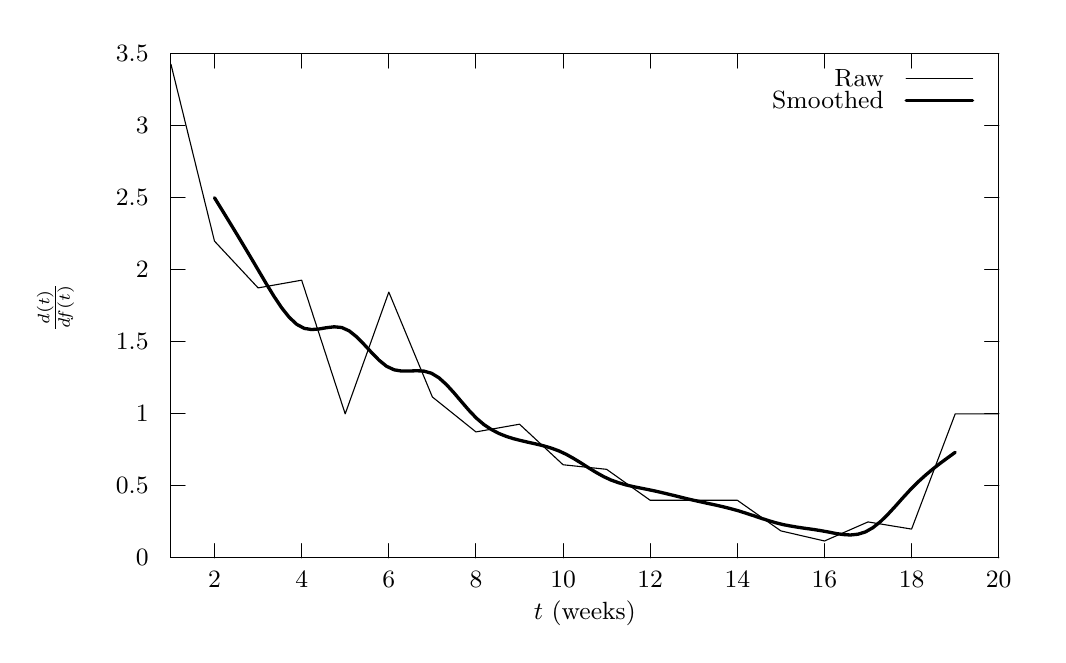
\begin{tikzpicture}[gnuplot]
%% generated with GNUPLOT 4.6p5 (Lua 5.2; terminal rev. 99, script rev. 100)
%% 2/09/2014 2:44:41 PM
\tikzset{every node/.append style={font={\fontsize{9pt}{10.8pt}\selectfont}}}
\gpmonochromelines
\path (0.000,0.000) rectangle (12.700,7.620);
\gpcolor{color=gp lt color border}
\gpsetlinetype{gp lt border}
\gpsetlinewidth{1.00}
\draw[gp path] (1.688,0.886)--(1.868,0.886);
\draw[gp path] (12.201,0.886)--(12.021,0.886);
\node[gp node right] at (1.522,0.886) { 0};
\draw[gp path] (1.688,1.800)--(1.868,1.800);
\draw[gp path] (12.201,1.800)--(12.021,1.800);
\node[gp node right] at (1.522,1.800) { 0.5};
\draw[gp path] (1.688,2.715)--(1.868,2.715);
\draw[gp path] (12.201,2.715)--(12.021,2.715);
\node[gp node right] at (1.522,2.715) { 1};
\draw[gp path] (1.688,3.629)--(1.868,3.629);
\draw[gp path] (12.201,3.629)--(12.021,3.629);
\node[gp node right] at (1.522,3.629) { 1.5};
\draw[gp path] (1.688,4.544)--(1.868,4.544);
\draw[gp path] (12.201,4.544)--(12.021,4.544);
\node[gp node right] at (1.522,4.544) { 2};
\draw[gp path] (1.688,5.458)--(1.868,5.458);
\draw[gp path] (12.201,5.458)--(12.021,5.458);
\node[gp node right] at (1.522,5.458) { 2.5};
\draw[gp path] (1.688,6.373)--(1.868,6.373);
\draw[gp path] (12.201,6.373)--(12.021,6.373);
\node[gp node right] at (1.522,6.373) { 3};
\draw[gp path] (1.688,7.287)--(1.868,7.287);
\draw[gp path] (12.201,7.287)--(12.021,7.287);
\node[gp node right] at (1.522,7.287) { 3.5};
\draw[gp path] (2.241,0.886)--(2.241,1.066);
\draw[gp path] (2.241,7.287)--(2.241,7.107);
\node[gp node center] at (2.241,0.609) { 2};
\draw[gp path] (3.348,0.886)--(3.348,1.066);
\draw[gp path] (3.348,7.287)--(3.348,7.107);
\node[gp node center] at (3.348,0.609) { 4};
\draw[gp path] (4.455,0.886)--(4.455,1.066);
\draw[gp path] (4.455,7.287)--(4.455,7.107);
\node[gp node center] at (4.455,0.609) { 6};
\draw[gp path] (5.561,0.886)--(5.561,1.066);
\draw[gp path] (5.561,7.287)--(5.561,7.107);
\node[gp node center] at (5.561,0.609) { 8};
\draw[gp path] (6.668,0.886)--(6.668,1.066);
\draw[gp path] (6.668,7.287)--(6.668,7.107);
\node[gp node center] at (6.668,0.609) { 10};
\draw[gp path] (7.774,0.886)--(7.774,1.066);
\draw[gp path] (7.774,7.287)--(7.774,7.107);
\node[gp node center] at (7.774,0.609) { 12};
\draw[gp path] (8.881,0.886)--(8.881,1.066);
\draw[gp path] (8.881,7.287)--(8.881,7.107);
\node[gp node center] at (8.881,0.609) { 14};
\draw[gp path] (9.988,0.886)--(9.988,1.066);
\draw[gp path] (9.988,7.287)--(9.988,7.107);
\node[gp node center] at (9.988,0.609) { 16};
\draw[gp path] (11.094,0.886)--(11.094,1.066);
\draw[gp path] (11.094,7.287)--(11.094,7.107);
\node[gp node center] at (11.094,0.609) { 18};
\draw[gp path] (12.201,0.886)--(12.201,1.066);
\draw[gp path] (12.201,7.287)--(12.201,7.107);
\node[gp node center] at (12.201,0.609) { 20};
\draw[gp path] (1.688,7.287)--(1.688,0.886)--(12.201,0.886)--(12.201,7.287)--cycle;
\node[gp node center,rotate=-270] at (0.221,4.086) {$\frac{d(t)}{df(t)}$};
\node[gp node center] at (6.944,0.194) {$t$ (weeks)};
\node[gp node right] at (10.859,6.969) {Raw};
\gpcolor{color=gp lt color 3}
\gpsetlinetype{gp lt plot 3}
\draw[gp path] (11.025,6.969)--(11.869,6.969);
\draw[gp path] (1.688,7.156)--(2.241,4.909)--(2.795,4.315)--(3.348,4.413)--(3.901,2.715)%
  --(4.455,4.262)--(5.008,2.930)--(5.561,2.486)--(6.115,2.584)--(6.668,2.069)--(7.221,2.011)%
  --(7.774,1.618)--(8.328,1.618)--(8.881,1.618)--(9.434,1.229)--(9.988,1.101)--(10.541,1.343)%
  --(11.094,1.252)--(11.648,2.715)--(12.201,2.715);
\gpcolor{color=gp lt color border}
\node[gp node right] at (10.859,6.692) {Smoothed};
\gpcolor{color=gp lt color 0}
\gpsetlinetype{gp lt plot 0}
\gpsetlinewidth{3.00}
\draw[gp path] (11.025,6.692)--(11.869,6.692);
\draw[gp path] (2.241,5.460)--(2.336,5.306)--(2.431,5.151)--(2.526,4.995)--(2.621,4.837)%
  --(2.716,4.678)--(2.811,4.517)--(2.906,4.356)--(3.001,4.201)--(3.096,4.060)--(3.191,3.941)%
  --(3.286,3.852)--(3.381,3.801)--(3.476,3.786)--(3.572,3.794)--(3.667,3.810)--(3.762,3.821)%
  --(3.857,3.812)--(3.952,3.769)--(4.047,3.693)--(4.142,3.596)--(4.237,3.493)--(4.332,3.396)%
  --(4.427,3.319)--(4.522,3.275)--(4.617,3.259)--(4.712,3.259)--(4.807,3.263)--(4.902,3.258)%
  --(4.997,3.231)--(5.092,3.173)--(5.187,3.087)--(5.282,2.983)--(5.377,2.871)--(5.472,2.761)%
  --(5.567,2.661)--(5.662,2.580)--(5.757,2.517)--(5.852,2.467)--(5.947,2.429)--(6.042,2.399)%
  --(6.137,2.375)--(6.232,2.353)--(6.327,2.332)--(6.422,2.309)--(6.517,2.281)--(6.612,2.246)%
  --(6.707,2.202)--(6.802,2.149)--(6.897,2.091)--(6.992,2.030)--(7.087,1.972)--(7.182,1.919)%
  --(7.277,1.875)--(7.372,1.841)--(7.467,1.813)--(7.562,1.791)--(7.657,1.772)--(7.752,1.753)%
  --(7.847,1.733)--(7.942,1.711)--(8.037,1.688)--(8.132,1.665)--(8.227,1.641)--(8.322,1.619)%
  --(8.417,1.598)--(8.512,1.577)--(8.607,1.557)--(8.702,1.535)--(8.797,1.511)--(8.892,1.485)%
  --(8.987,1.455)--(9.082,1.424)--(9.177,1.392)--(9.272,1.361)--(9.367,1.333)--(9.462,1.309)%
  --(9.557,1.291)--(9.652,1.275)--(9.747,1.261)--(9.842,1.248)--(9.937,1.233)--(10.032,1.216)%
  --(10.127,1.197)--(10.222,1.183)--(10.317,1.177)--(10.413,1.187)--(10.508,1.216)--(10.603,1.270)%
  --(10.698,1.346)--(10.793,1.439)--(10.888,1.542)--(10.983,1.649)--(11.078,1.752)--(11.173,1.848)%
  --(11.268,1.934)--(11.363,2.014)--(11.458,2.088)--(11.553,2.158)--(11.648,2.227);
\gpcolor{color=gp lt color border}
\gpsetlinetype{gp lt border}
\gpsetlinewidth{1.00}
\draw[gp path] (1.688,7.287)--(1.688,0.886)--(12.201,0.886)--(12.201,7.287)--cycle;
%% coordinates of the plot area
\gpdefrectangularnode{gp plot 1}{\pgfpoint{1.688cm}{0.886cm}}{\pgfpoint{12.201cm}{7.287cm}}
\end{tikzpicture}
%% gnuplot variables

    \caption{Scenario B Result}
  \end{figure}
  
  \begin{figure}[!htb]
    \centering
    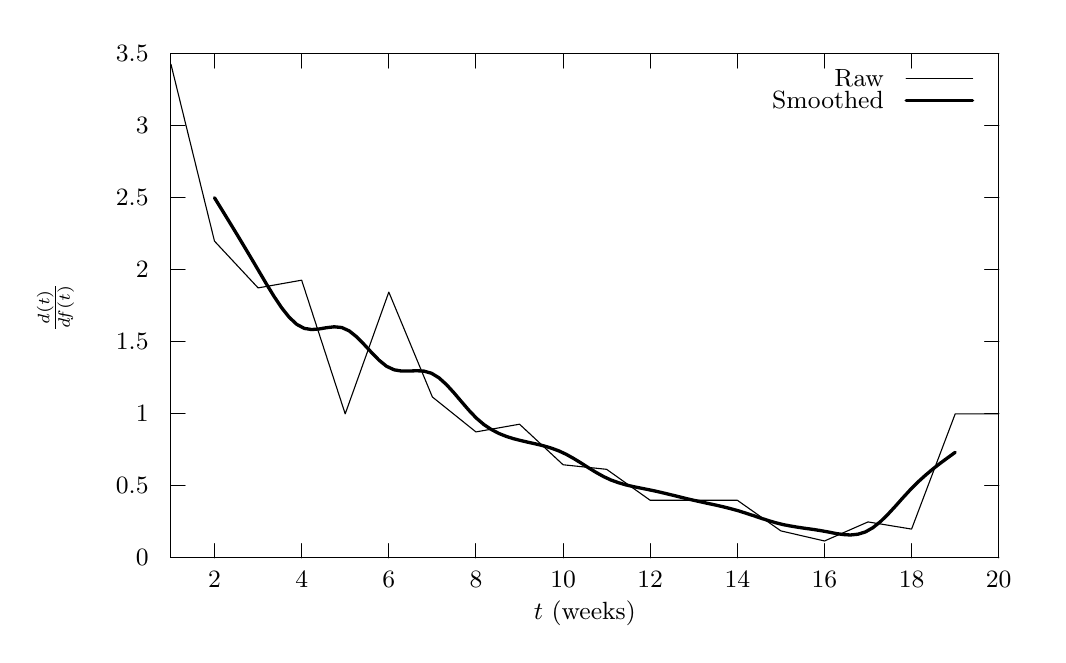
\begin{tikzpicture}[gnuplot]
%% generated with GNUPLOT 4.6p5 (Lua 5.2; terminal rev. 99, script rev. 100)
%% 2/09/2014 2:44:41 PM
\tikzset{every node/.append style={font={\fontsize{9pt}{10.8pt}\selectfont}}}
\gpmonochromelines
\path (0.000,0.000) rectangle (12.700,7.620);
\gpcolor{color=gp lt color border}
\gpsetlinetype{gp lt border}
\gpsetlinewidth{1.00}
\draw[gp path] (1.688,0.886)--(1.868,0.886);
\draw[gp path] (12.201,0.886)--(12.021,0.886);
\node[gp node right] at (1.522,0.886) { 0};
\draw[gp path] (1.688,1.800)--(1.868,1.800);
\draw[gp path] (12.201,1.800)--(12.021,1.800);
\node[gp node right] at (1.522,1.800) { 0.5};
\draw[gp path] (1.688,2.715)--(1.868,2.715);
\draw[gp path] (12.201,2.715)--(12.021,2.715);
\node[gp node right] at (1.522,2.715) { 1};
\draw[gp path] (1.688,3.629)--(1.868,3.629);
\draw[gp path] (12.201,3.629)--(12.021,3.629);
\node[gp node right] at (1.522,3.629) { 1.5};
\draw[gp path] (1.688,4.544)--(1.868,4.544);
\draw[gp path] (12.201,4.544)--(12.021,4.544);
\node[gp node right] at (1.522,4.544) { 2};
\draw[gp path] (1.688,5.458)--(1.868,5.458);
\draw[gp path] (12.201,5.458)--(12.021,5.458);
\node[gp node right] at (1.522,5.458) { 2.5};
\draw[gp path] (1.688,6.373)--(1.868,6.373);
\draw[gp path] (12.201,6.373)--(12.021,6.373);
\node[gp node right] at (1.522,6.373) { 3};
\draw[gp path] (1.688,7.287)--(1.868,7.287);
\draw[gp path] (12.201,7.287)--(12.021,7.287);
\node[gp node right] at (1.522,7.287) { 3.5};
\draw[gp path] (2.241,0.886)--(2.241,1.066);
\draw[gp path] (2.241,7.287)--(2.241,7.107);
\node[gp node center] at (2.241,0.609) { 2};
\draw[gp path] (3.348,0.886)--(3.348,1.066);
\draw[gp path] (3.348,7.287)--(3.348,7.107);
\node[gp node center] at (3.348,0.609) { 4};
\draw[gp path] (4.455,0.886)--(4.455,1.066);
\draw[gp path] (4.455,7.287)--(4.455,7.107);
\node[gp node center] at (4.455,0.609) { 6};
\draw[gp path] (5.561,0.886)--(5.561,1.066);
\draw[gp path] (5.561,7.287)--(5.561,7.107);
\node[gp node center] at (5.561,0.609) { 8};
\draw[gp path] (6.668,0.886)--(6.668,1.066);
\draw[gp path] (6.668,7.287)--(6.668,7.107);
\node[gp node center] at (6.668,0.609) { 10};
\draw[gp path] (7.774,0.886)--(7.774,1.066);
\draw[gp path] (7.774,7.287)--(7.774,7.107);
\node[gp node center] at (7.774,0.609) { 12};
\draw[gp path] (8.881,0.886)--(8.881,1.066);
\draw[gp path] (8.881,7.287)--(8.881,7.107);
\node[gp node center] at (8.881,0.609) { 14};
\draw[gp path] (9.988,0.886)--(9.988,1.066);
\draw[gp path] (9.988,7.287)--(9.988,7.107);
\node[gp node center] at (9.988,0.609) { 16};
\draw[gp path] (11.094,0.886)--(11.094,1.066);
\draw[gp path] (11.094,7.287)--(11.094,7.107);
\node[gp node center] at (11.094,0.609) { 18};
\draw[gp path] (12.201,0.886)--(12.201,1.066);
\draw[gp path] (12.201,7.287)--(12.201,7.107);
\node[gp node center] at (12.201,0.609) { 20};
\draw[gp path] (1.688,7.287)--(1.688,0.886)--(12.201,0.886)--(12.201,7.287)--cycle;
\node[gp node center,rotate=-270] at (0.221,4.086) {$\frac{d(t)}{df(t)}$};
\node[gp node center] at (6.944,0.194) {$t$ (weeks)};
\node[gp node right] at (10.859,6.969) {Raw};
\gpcolor{color=gp lt color 3}
\gpsetlinetype{gp lt plot 3}
\draw[gp path] (11.025,6.969)--(11.869,6.969);
\draw[gp path] (1.688,7.156)--(2.241,4.909)--(2.795,4.315)--(3.348,4.413)--(3.901,2.715)%
  --(4.455,4.262)--(5.008,2.930)--(5.561,2.486)--(6.115,2.584)--(6.668,2.069)--(7.221,2.011)%
  --(7.774,1.618)--(8.328,1.618)--(8.881,1.618)--(9.434,1.229)--(9.988,1.101)--(10.541,1.343)%
  --(11.094,1.252)--(11.648,2.715)--(12.201,2.715);
\gpcolor{color=gp lt color border}
\node[gp node right] at (10.859,6.692) {Smoothed};
\gpcolor{color=gp lt color 0}
\gpsetlinetype{gp lt plot 0}
\gpsetlinewidth{3.00}
\draw[gp path] (11.025,6.692)--(11.869,6.692);
\draw[gp path] (2.241,5.460)--(2.336,5.306)--(2.431,5.151)--(2.526,4.995)--(2.621,4.837)%
  --(2.716,4.678)--(2.811,4.517)--(2.906,4.356)--(3.001,4.201)--(3.096,4.060)--(3.191,3.941)%
  --(3.286,3.852)--(3.381,3.801)--(3.476,3.786)--(3.572,3.794)--(3.667,3.810)--(3.762,3.821)%
  --(3.857,3.812)--(3.952,3.769)--(4.047,3.693)--(4.142,3.596)--(4.237,3.493)--(4.332,3.396)%
  --(4.427,3.319)--(4.522,3.275)--(4.617,3.259)--(4.712,3.259)--(4.807,3.263)--(4.902,3.258)%
  --(4.997,3.231)--(5.092,3.173)--(5.187,3.087)--(5.282,2.983)--(5.377,2.871)--(5.472,2.761)%
  --(5.567,2.661)--(5.662,2.580)--(5.757,2.517)--(5.852,2.467)--(5.947,2.429)--(6.042,2.399)%
  --(6.137,2.375)--(6.232,2.353)--(6.327,2.332)--(6.422,2.309)--(6.517,2.281)--(6.612,2.246)%
  --(6.707,2.202)--(6.802,2.149)--(6.897,2.091)--(6.992,2.030)--(7.087,1.972)--(7.182,1.919)%
  --(7.277,1.875)--(7.372,1.841)--(7.467,1.813)--(7.562,1.791)--(7.657,1.772)--(7.752,1.753)%
  --(7.847,1.733)--(7.942,1.711)--(8.037,1.688)--(8.132,1.665)--(8.227,1.641)--(8.322,1.619)%
  --(8.417,1.598)--(8.512,1.577)--(8.607,1.557)--(8.702,1.535)--(8.797,1.511)--(8.892,1.485)%
  --(8.987,1.455)--(9.082,1.424)--(9.177,1.392)--(9.272,1.361)--(9.367,1.333)--(9.462,1.309)%
  --(9.557,1.291)--(9.652,1.275)--(9.747,1.261)--(9.842,1.248)--(9.937,1.233)--(10.032,1.216)%
  --(10.127,1.197)--(10.222,1.183)--(10.317,1.177)--(10.413,1.187)--(10.508,1.216)--(10.603,1.270)%
  --(10.698,1.346)--(10.793,1.439)--(10.888,1.542)--(10.983,1.649)--(11.078,1.752)--(11.173,1.848)%
  --(11.268,1.934)--(11.363,2.014)--(11.458,2.088)--(11.553,2.158)--(11.648,2.227);
\gpcolor{color=gp lt color border}
\gpsetlinetype{gp lt border}
\gpsetlinewidth{1.00}
\draw[gp path] (1.688,7.287)--(1.688,0.886)--(12.201,0.886)--(12.201,7.287)--cycle;
%% coordinates of the plot area
\gpdefrectangularnode{gp plot 1}{\pgfpoint{1.688cm}{0.886cm}}{\pgfpoint{12.201cm}{7.287cm}}
\end{tikzpicture}
%% gnuplot variables

    \caption{Scenario C Result}
  \end{figure}
  
  \begin{figure}[!htb]
    \centering
    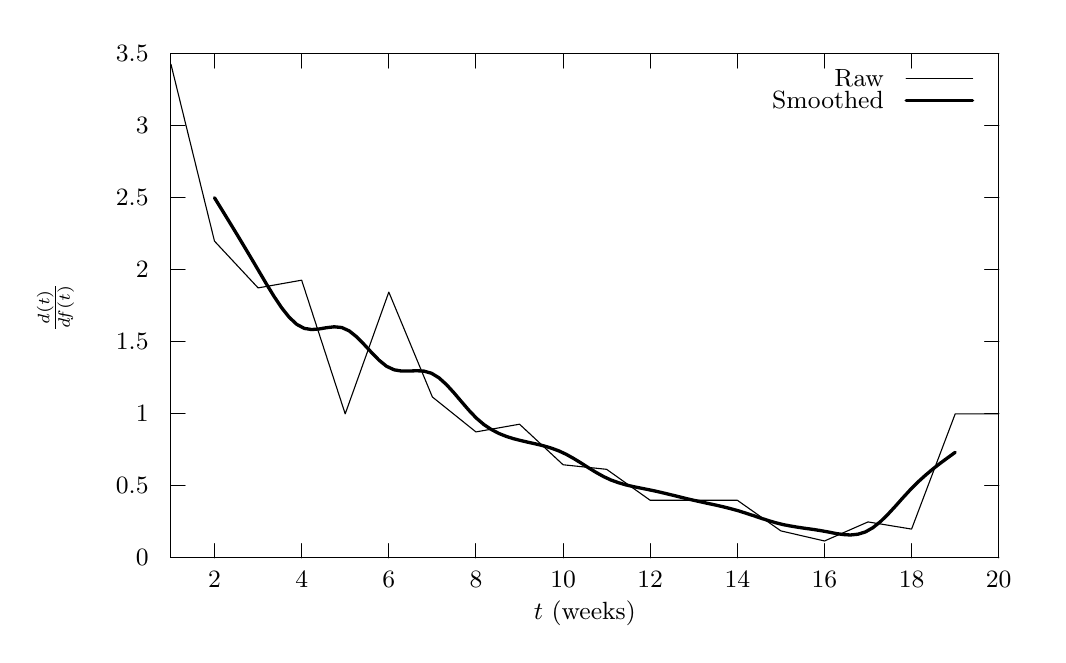
\begin{tikzpicture}[gnuplot]
%% generated with GNUPLOT 4.6p5 (Lua 5.2; terminal rev. 99, script rev. 100)
%% 2/09/2014 2:44:41 PM
\tikzset{every node/.append style={font={\fontsize{9pt}{10.8pt}\selectfont}}}
\gpmonochromelines
\path (0.000,0.000) rectangle (12.700,7.620);
\gpcolor{color=gp lt color border}
\gpsetlinetype{gp lt border}
\gpsetlinewidth{1.00}
\draw[gp path] (1.688,0.886)--(1.868,0.886);
\draw[gp path] (12.201,0.886)--(12.021,0.886);
\node[gp node right] at (1.522,0.886) { 0};
\draw[gp path] (1.688,1.800)--(1.868,1.800);
\draw[gp path] (12.201,1.800)--(12.021,1.800);
\node[gp node right] at (1.522,1.800) { 0.5};
\draw[gp path] (1.688,2.715)--(1.868,2.715);
\draw[gp path] (12.201,2.715)--(12.021,2.715);
\node[gp node right] at (1.522,2.715) { 1};
\draw[gp path] (1.688,3.629)--(1.868,3.629);
\draw[gp path] (12.201,3.629)--(12.021,3.629);
\node[gp node right] at (1.522,3.629) { 1.5};
\draw[gp path] (1.688,4.544)--(1.868,4.544);
\draw[gp path] (12.201,4.544)--(12.021,4.544);
\node[gp node right] at (1.522,4.544) { 2};
\draw[gp path] (1.688,5.458)--(1.868,5.458);
\draw[gp path] (12.201,5.458)--(12.021,5.458);
\node[gp node right] at (1.522,5.458) { 2.5};
\draw[gp path] (1.688,6.373)--(1.868,6.373);
\draw[gp path] (12.201,6.373)--(12.021,6.373);
\node[gp node right] at (1.522,6.373) { 3};
\draw[gp path] (1.688,7.287)--(1.868,7.287);
\draw[gp path] (12.201,7.287)--(12.021,7.287);
\node[gp node right] at (1.522,7.287) { 3.5};
\draw[gp path] (2.241,0.886)--(2.241,1.066);
\draw[gp path] (2.241,7.287)--(2.241,7.107);
\node[gp node center] at (2.241,0.609) { 2};
\draw[gp path] (3.348,0.886)--(3.348,1.066);
\draw[gp path] (3.348,7.287)--(3.348,7.107);
\node[gp node center] at (3.348,0.609) { 4};
\draw[gp path] (4.455,0.886)--(4.455,1.066);
\draw[gp path] (4.455,7.287)--(4.455,7.107);
\node[gp node center] at (4.455,0.609) { 6};
\draw[gp path] (5.561,0.886)--(5.561,1.066);
\draw[gp path] (5.561,7.287)--(5.561,7.107);
\node[gp node center] at (5.561,0.609) { 8};
\draw[gp path] (6.668,0.886)--(6.668,1.066);
\draw[gp path] (6.668,7.287)--(6.668,7.107);
\node[gp node center] at (6.668,0.609) { 10};
\draw[gp path] (7.774,0.886)--(7.774,1.066);
\draw[gp path] (7.774,7.287)--(7.774,7.107);
\node[gp node center] at (7.774,0.609) { 12};
\draw[gp path] (8.881,0.886)--(8.881,1.066);
\draw[gp path] (8.881,7.287)--(8.881,7.107);
\node[gp node center] at (8.881,0.609) { 14};
\draw[gp path] (9.988,0.886)--(9.988,1.066);
\draw[gp path] (9.988,7.287)--(9.988,7.107);
\node[gp node center] at (9.988,0.609) { 16};
\draw[gp path] (11.094,0.886)--(11.094,1.066);
\draw[gp path] (11.094,7.287)--(11.094,7.107);
\node[gp node center] at (11.094,0.609) { 18};
\draw[gp path] (12.201,0.886)--(12.201,1.066);
\draw[gp path] (12.201,7.287)--(12.201,7.107);
\node[gp node center] at (12.201,0.609) { 20};
\draw[gp path] (1.688,7.287)--(1.688,0.886)--(12.201,0.886)--(12.201,7.287)--cycle;
\node[gp node center,rotate=-270] at (0.221,4.086) {$\frac{d(t)}{df(t)}$};
\node[gp node center] at (6.944,0.194) {$t$ (weeks)};
\node[gp node right] at (10.859,6.969) {Raw};
\gpcolor{color=gp lt color 3}
\gpsetlinetype{gp lt plot 3}
\draw[gp path] (11.025,6.969)--(11.869,6.969);
\draw[gp path] (1.688,7.156)--(2.241,4.909)--(2.795,4.315)--(3.348,4.413)--(3.901,2.715)%
  --(4.455,4.262)--(5.008,2.930)--(5.561,2.486)--(6.115,2.584)--(6.668,2.069)--(7.221,2.011)%
  --(7.774,1.618)--(8.328,1.618)--(8.881,1.618)--(9.434,1.229)--(9.988,1.101)--(10.541,1.343)%
  --(11.094,1.252)--(11.648,2.715)--(12.201,2.715);
\gpcolor{color=gp lt color border}
\node[gp node right] at (10.859,6.692) {Smoothed};
\gpcolor{color=gp lt color 0}
\gpsetlinetype{gp lt plot 0}
\gpsetlinewidth{3.00}
\draw[gp path] (11.025,6.692)--(11.869,6.692);
\draw[gp path] (2.241,5.460)--(2.336,5.306)--(2.431,5.151)--(2.526,4.995)--(2.621,4.837)%
  --(2.716,4.678)--(2.811,4.517)--(2.906,4.356)--(3.001,4.201)--(3.096,4.060)--(3.191,3.941)%
  --(3.286,3.852)--(3.381,3.801)--(3.476,3.786)--(3.572,3.794)--(3.667,3.810)--(3.762,3.821)%
  --(3.857,3.812)--(3.952,3.769)--(4.047,3.693)--(4.142,3.596)--(4.237,3.493)--(4.332,3.396)%
  --(4.427,3.319)--(4.522,3.275)--(4.617,3.259)--(4.712,3.259)--(4.807,3.263)--(4.902,3.258)%
  --(4.997,3.231)--(5.092,3.173)--(5.187,3.087)--(5.282,2.983)--(5.377,2.871)--(5.472,2.761)%
  --(5.567,2.661)--(5.662,2.580)--(5.757,2.517)--(5.852,2.467)--(5.947,2.429)--(6.042,2.399)%
  --(6.137,2.375)--(6.232,2.353)--(6.327,2.332)--(6.422,2.309)--(6.517,2.281)--(6.612,2.246)%
  --(6.707,2.202)--(6.802,2.149)--(6.897,2.091)--(6.992,2.030)--(7.087,1.972)--(7.182,1.919)%
  --(7.277,1.875)--(7.372,1.841)--(7.467,1.813)--(7.562,1.791)--(7.657,1.772)--(7.752,1.753)%
  --(7.847,1.733)--(7.942,1.711)--(8.037,1.688)--(8.132,1.665)--(8.227,1.641)--(8.322,1.619)%
  --(8.417,1.598)--(8.512,1.577)--(8.607,1.557)--(8.702,1.535)--(8.797,1.511)--(8.892,1.485)%
  --(8.987,1.455)--(9.082,1.424)--(9.177,1.392)--(9.272,1.361)--(9.367,1.333)--(9.462,1.309)%
  --(9.557,1.291)--(9.652,1.275)--(9.747,1.261)--(9.842,1.248)--(9.937,1.233)--(10.032,1.216)%
  --(10.127,1.197)--(10.222,1.183)--(10.317,1.177)--(10.413,1.187)--(10.508,1.216)--(10.603,1.270)%
  --(10.698,1.346)--(10.793,1.439)--(10.888,1.542)--(10.983,1.649)--(11.078,1.752)--(11.173,1.848)%
  --(11.268,1.934)--(11.363,2.014)--(11.458,2.088)--(11.553,2.158)--(11.648,2.227);
\gpcolor{color=gp lt color border}
\gpsetlinetype{gp lt border}
\gpsetlinewidth{1.00}
\draw[gp path] (1.688,7.287)--(1.688,0.886)--(12.201,0.886)--(12.201,7.287)--cycle;
%% coordinates of the plot area
\gpdefrectangularnode{gp plot 1}{\pgfpoint{1.688cm}{0.886cm}}{\pgfpoint{12.201cm}{7.287cm}}
\end{tikzpicture}
%% gnuplot variables

    \caption{Scenario D Result}
  \end{figure}
  
  \clearpage
  \subsection{Total importance of found defects still to be fixed}
  \begin{figure}[!htb]
    \centering
    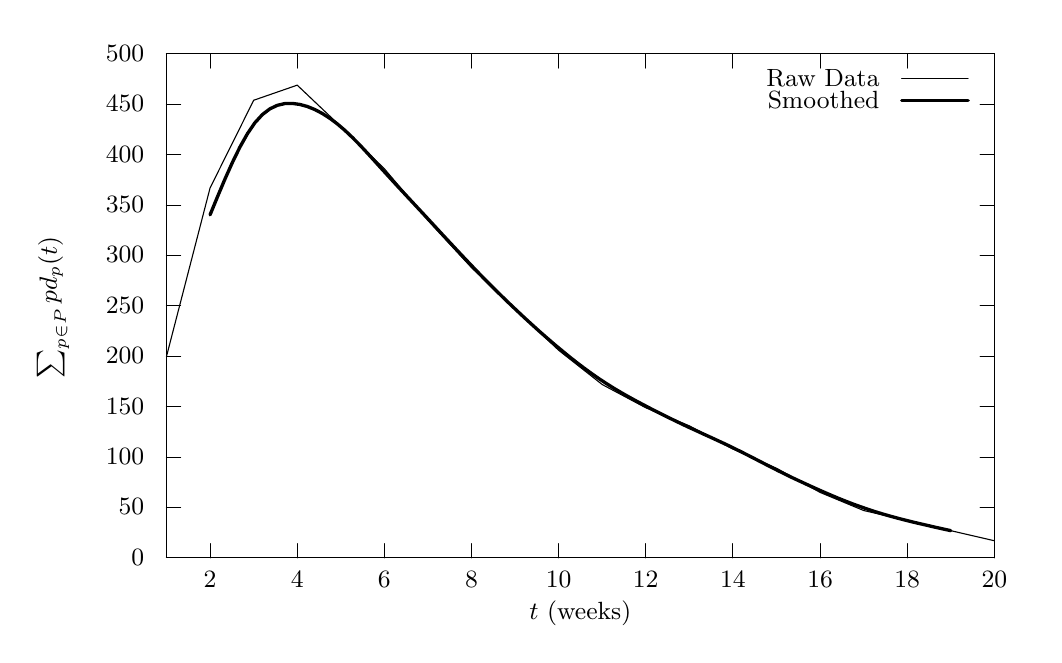
\begin{tikzpicture}[gnuplot]
%% generated with GNUPLOT 4.6p4 (Lua 5.1; terminal rev. 99, script rev. 100)
%% Thu 04 Sep 2014 10:50:27 WST
\tikzset{every node/.append style={font={\fontsize{9pt}{10.8pt}\selectfont}}}
\gpmonochromelines
\path (0.000,0.000) rectangle (12.700,7.620);
\gpcolor{color=gp lt color border}
\gpsetlinetype{gp lt border}
\gpsetlinewidth{1.00}
\draw[gp path] (1.688,0.886)--(1.868,0.886);
\draw[gp path] (12.201,0.886)--(12.021,0.886);
\node[gp node right] at (1.522,0.886) { 0};
\draw[gp path] (1.688,1.526)--(1.868,1.526);
\draw[gp path] (12.201,1.526)--(12.021,1.526);
\node[gp node right] at (1.522,1.526) { 50};
\draw[gp path] (1.688,2.166)--(1.868,2.166);
\draw[gp path] (12.201,2.166)--(12.021,2.166);
\node[gp node right] at (1.522,2.166) { 100};
\draw[gp path] (1.688,2.806)--(1.868,2.806);
\draw[gp path] (12.201,2.806)--(12.021,2.806);
\node[gp node right] at (1.522,2.806) { 150};
\draw[gp path] (1.688,3.446)--(1.868,3.446);
\draw[gp path] (12.201,3.446)--(12.021,3.446);
\node[gp node right] at (1.522,3.446) { 200};
\draw[gp path] (1.688,4.087)--(1.868,4.087);
\draw[gp path] (12.201,4.087)--(12.021,4.087);
\node[gp node right] at (1.522,4.087) { 250};
\draw[gp path] (1.688,4.727)--(1.868,4.727);
\draw[gp path] (12.201,4.727)--(12.021,4.727);
\node[gp node right] at (1.522,4.727) { 300};
\draw[gp path] (1.688,5.367)--(1.868,5.367);
\draw[gp path] (12.201,5.367)--(12.021,5.367);
\node[gp node right] at (1.522,5.367) { 350};
\draw[gp path] (1.688,6.007)--(1.868,6.007);
\draw[gp path] (12.201,6.007)--(12.021,6.007);
\node[gp node right] at (1.522,6.007) { 400};
\draw[gp path] (1.688,6.647)--(1.868,6.647);
\draw[gp path] (12.201,6.647)--(12.021,6.647);
\node[gp node right] at (1.522,6.647) { 450};
\draw[gp path] (1.688,7.287)--(1.868,7.287);
\draw[gp path] (12.201,7.287)--(12.021,7.287);
\node[gp node right] at (1.522,7.287) { 500};
\draw[gp path] (2.241,0.886)--(2.241,1.066);
\draw[gp path] (2.241,7.287)--(2.241,7.107);
\node[gp node center] at (2.241,0.609) { 2};
\draw[gp path] (3.348,0.886)--(3.348,1.066);
\draw[gp path] (3.348,7.287)--(3.348,7.107);
\node[gp node center] at (3.348,0.609) { 4};
\draw[gp path] (4.455,0.886)--(4.455,1.066);
\draw[gp path] (4.455,7.287)--(4.455,7.107);
\node[gp node center] at (4.455,0.609) { 6};
\draw[gp path] (5.561,0.886)--(5.561,1.066);
\draw[gp path] (5.561,7.287)--(5.561,7.107);
\node[gp node center] at (5.561,0.609) { 8};
\draw[gp path] (6.668,0.886)--(6.668,1.066);
\draw[gp path] (6.668,7.287)--(6.668,7.107);
\node[gp node center] at (6.668,0.609) { 10};
\draw[gp path] (7.774,0.886)--(7.774,1.066);
\draw[gp path] (7.774,7.287)--(7.774,7.107);
\node[gp node center] at (7.774,0.609) { 12};
\draw[gp path] (8.881,0.886)--(8.881,1.066);
\draw[gp path] (8.881,7.287)--(8.881,7.107);
\node[gp node center] at (8.881,0.609) { 14};
\draw[gp path] (9.988,0.886)--(9.988,1.066);
\draw[gp path] (9.988,7.287)--(9.988,7.107);
\node[gp node center] at (9.988,0.609) { 16};
\draw[gp path] (11.094,0.886)--(11.094,1.066);
\draw[gp path] (11.094,7.287)--(11.094,7.107);
\node[gp node center] at (11.094,0.609) { 18};
\draw[gp path] (12.201,0.886)--(12.201,1.066);
\draw[gp path] (12.201,7.287)--(12.201,7.107);
\node[gp node center] at (12.201,0.609) { 20};
\draw[gp path] (1.688,7.287)--(1.688,0.886)--(12.201,0.886)--(12.201,7.287)--cycle;
\node[gp node center,rotate=-270] at (0.221,4.086) {$\sum_{p \in P} p d_p(t)$};
\node[gp node center] at (6.944,0.194) {$t$ (weeks)};
\node[gp node right] at (10.859,6.969) {Raw Data};
\gpcolor{color=gp lt color 3}
\gpsetlinetype{gp lt plot 3}
\draw[gp path] (11.025,6.969)--(11.869,6.969);
\draw[gp path] (1.688,3.446)--(2.241,5.584)--(2.795,6.698)--(3.348,6.890)--(3.901,6.365)%
  --(4.455,5.828)--(5.008,5.175)--(5.561,4.573)--(6.115,4.048)--(6.668,3.523)--(7.221,3.088)%
  --(7.774,2.793)--(8.328,2.563)--(8.881,2.269)--(9.434,2.025)--(9.988,1.718)--(10.541,1.488)%
  --(11.094,1.360)--(11.648,1.232)--(12.201,1.104);
\gpcolor{color=gp lt color border}
\node[gp node right] at (10.859,6.692) {Smoothed};
\gpcolor{color=gp lt color 0}
\gpsetlinetype{gp lt plot 0}
\gpsetlinewidth{3.00}
\draw[gp path] (11.025,6.692)--(11.869,6.692);
\draw[gp path] (2.241,5.243)--(2.336,5.474)--(2.431,5.699)--(2.526,5.911)--(2.621,6.105)%
  --(2.716,6.274)--(2.811,6.413)--(2.906,6.517)--(3.001,6.589)--(3.096,6.634)--(3.191,6.656)%
  --(3.286,6.658)--(3.381,6.645)--(3.476,6.619)--(3.572,6.580)--(3.667,6.530)--(3.762,6.469)%
  --(3.857,6.398)--(3.952,6.317)--(4.047,6.227)--(4.142,6.131)--(4.237,6.029)--(4.332,5.925)%
  --(4.427,5.820)--(4.522,5.716)--(4.617,5.612)--(4.712,5.510)--(4.807,5.408)--(4.902,5.306)%
  --(4.997,5.204)--(5.092,5.101)--(5.187,4.998)--(5.282,4.896)--(5.377,4.794)--(5.472,4.693)%
  --(5.567,4.593)--(5.662,4.494)--(5.757,4.398)--(5.852,4.303)--(5.947,4.209)--(6.042,4.117)%
  --(6.137,4.027)--(6.232,3.938)--(6.327,3.851)--(6.422,3.765)--(6.517,3.682)--(6.612,3.600)%
  --(6.707,3.521)--(6.802,3.443)--(6.897,3.368)--(6.992,3.296)--(7.087,3.227)--(7.182,3.161)%
  --(7.277,3.099)--(7.372,3.039)--(7.467,2.983)--(7.562,2.929)--(7.657,2.877)--(7.752,2.827)%
  --(7.847,2.777)--(7.942,2.729)--(8.037,2.681)--(8.132,2.635)--(8.227,2.589)--(8.322,2.544)%
  --(8.417,2.501)--(8.512,2.457)--(8.607,2.414)--(8.702,2.370)--(8.797,2.326)--(8.892,2.280)%
  --(8.987,2.233)--(9.082,2.185)--(9.177,2.136)--(9.272,2.087)--(9.367,2.038)--(9.462,1.990)%
  --(9.557,1.943)--(9.652,1.897)--(9.747,1.853)--(9.842,1.809)--(9.937,1.766)--(10.032,1.724)%
  --(10.127,1.683)--(10.222,1.643)--(10.317,1.605)--(10.413,1.568)--(10.508,1.534)--(10.603,1.501)%
  --(10.698,1.470)--(10.793,1.441)--(10.888,1.414)--(10.983,1.388)--(11.078,1.364)--(11.173,1.340)%
  --(11.268,1.318)--(11.363,1.296)--(11.458,1.274)--(11.553,1.253)--(11.648,1.232);
\gpcolor{color=gp lt color border}
\gpsetlinetype{gp lt border}
\gpsetlinewidth{1.00}
\draw[gp path] (1.688,7.287)--(1.688,0.886)--(12.201,0.886)--(12.201,7.287)--cycle;
%% coordinates of the plot area
\gpdefrectangularnode{gp plot 1}{\pgfpoint{1.688cm}{0.886cm}}{\pgfpoint{12.201cm}{7.287cm}}
\end{tikzpicture}
%% gnuplot variables

    \caption{Scenario B Result}
  \end{figure}
  
  \begin{figure}[!htb]
    \centering
    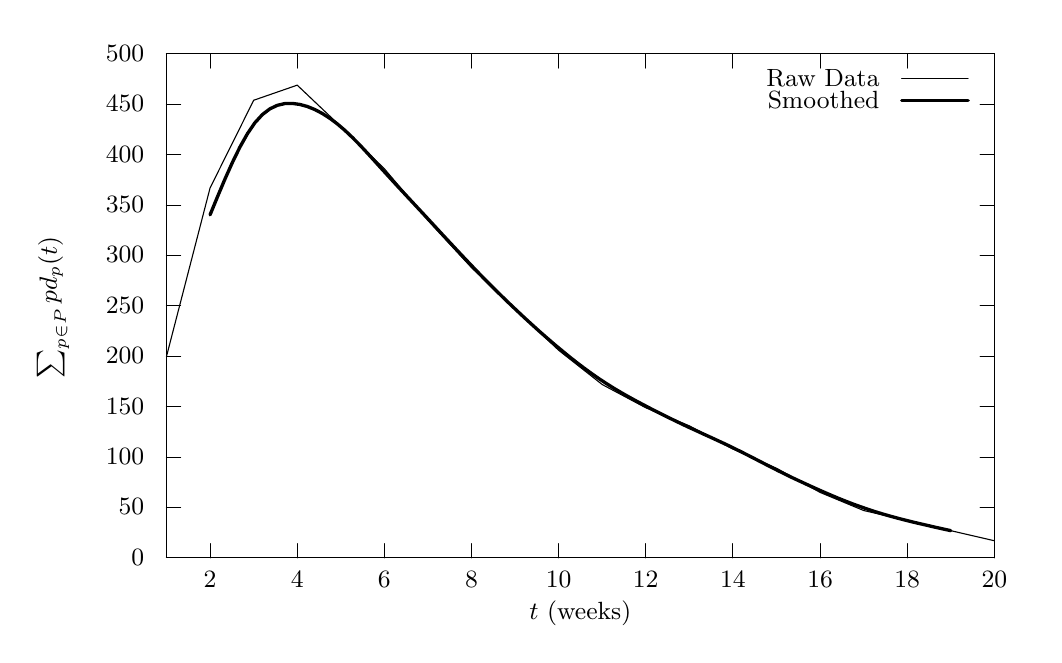
\begin{tikzpicture}[gnuplot]
%% generated with GNUPLOT 4.6p4 (Lua 5.1; terminal rev. 99, script rev. 100)
%% Thu 04 Sep 2014 10:50:27 WST
\tikzset{every node/.append style={font={\fontsize{9pt}{10.8pt}\selectfont}}}
\gpmonochromelines
\path (0.000,0.000) rectangle (12.700,7.620);
\gpcolor{color=gp lt color border}
\gpsetlinetype{gp lt border}
\gpsetlinewidth{1.00}
\draw[gp path] (1.688,0.886)--(1.868,0.886);
\draw[gp path] (12.201,0.886)--(12.021,0.886);
\node[gp node right] at (1.522,0.886) { 0};
\draw[gp path] (1.688,1.526)--(1.868,1.526);
\draw[gp path] (12.201,1.526)--(12.021,1.526);
\node[gp node right] at (1.522,1.526) { 50};
\draw[gp path] (1.688,2.166)--(1.868,2.166);
\draw[gp path] (12.201,2.166)--(12.021,2.166);
\node[gp node right] at (1.522,2.166) { 100};
\draw[gp path] (1.688,2.806)--(1.868,2.806);
\draw[gp path] (12.201,2.806)--(12.021,2.806);
\node[gp node right] at (1.522,2.806) { 150};
\draw[gp path] (1.688,3.446)--(1.868,3.446);
\draw[gp path] (12.201,3.446)--(12.021,3.446);
\node[gp node right] at (1.522,3.446) { 200};
\draw[gp path] (1.688,4.087)--(1.868,4.087);
\draw[gp path] (12.201,4.087)--(12.021,4.087);
\node[gp node right] at (1.522,4.087) { 250};
\draw[gp path] (1.688,4.727)--(1.868,4.727);
\draw[gp path] (12.201,4.727)--(12.021,4.727);
\node[gp node right] at (1.522,4.727) { 300};
\draw[gp path] (1.688,5.367)--(1.868,5.367);
\draw[gp path] (12.201,5.367)--(12.021,5.367);
\node[gp node right] at (1.522,5.367) { 350};
\draw[gp path] (1.688,6.007)--(1.868,6.007);
\draw[gp path] (12.201,6.007)--(12.021,6.007);
\node[gp node right] at (1.522,6.007) { 400};
\draw[gp path] (1.688,6.647)--(1.868,6.647);
\draw[gp path] (12.201,6.647)--(12.021,6.647);
\node[gp node right] at (1.522,6.647) { 450};
\draw[gp path] (1.688,7.287)--(1.868,7.287);
\draw[gp path] (12.201,7.287)--(12.021,7.287);
\node[gp node right] at (1.522,7.287) { 500};
\draw[gp path] (2.241,0.886)--(2.241,1.066);
\draw[gp path] (2.241,7.287)--(2.241,7.107);
\node[gp node center] at (2.241,0.609) { 2};
\draw[gp path] (3.348,0.886)--(3.348,1.066);
\draw[gp path] (3.348,7.287)--(3.348,7.107);
\node[gp node center] at (3.348,0.609) { 4};
\draw[gp path] (4.455,0.886)--(4.455,1.066);
\draw[gp path] (4.455,7.287)--(4.455,7.107);
\node[gp node center] at (4.455,0.609) { 6};
\draw[gp path] (5.561,0.886)--(5.561,1.066);
\draw[gp path] (5.561,7.287)--(5.561,7.107);
\node[gp node center] at (5.561,0.609) { 8};
\draw[gp path] (6.668,0.886)--(6.668,1.066);
\draw[gp path] (6.668,7.287)--(6.668,7.107);
\node[gp node center] at (6.668,0.609) { 10};
\draw[gp path] (7.774,0.886)--(7.774,1.066);
\draw[gp path] (7.774,7.287)--(7.774,7.107);
\node[gp node center] at (7.774,0.609) { 12};
\draw[gp path] (8.881,0.886)--(8.881,1.066);
\draw[gp path] (8.881,7.287)--(8.881,7.107);
\node[gp node center] at (8.881,0.609) { 14};
\draw[gp path] (9.988,0.886)--(9.988,1.066);
\draw[gp path] (9.988,7.287)--(9.988,7.107);
\node[gp node center] at (9.988,0.609) { 16};
\draw[gp path] (11.094,0.886)--(11.094,1.066);
\draw[gp path] (11.094,7.287)--(11.094,7.107);
\node[gp node center] at (11.094,0.609) { 18};
\draw[gp path] (12.201,0.886)--(12.201,1.066);
\draw[gp path] (12.201,7.287)--(12.201,7.107);
\node[gp node center] at (12.201,0.609) { 20};
\draw[gp path] (1.688,7.287)--(1.688,0.886)--(12.201,0.886)--(12.201,7.287)--cycle;
\node[gp node center,rotate=-270] at (0.221,4.086) {$\sum_{p \in P} p d_p(t)$};
\node[gp node center] at (6.944,0.194) {$t$ (weeks)};
\node[gp node right] at (10.859,6.969) {Raw Data};
\gpcolor{color=gp lt color 3}
\gpsetlinetype{gp lt plot 3}
\draw[gp path] (11.025,6.969)--(11.869,6.969);
\draw[gp path] (1.688,3.446)--(2.241,5.584)--(2.795,6.698)--(3.348,6.890)--(3.901,6.365)%
  --(4.455,5.828)--(5.008,5.175)--(5.561,4.573)--(6.115,4.048)--(6.668,3.523)--(7.221,3.088)%
  --(7.774,2.793)--(8.328,2.563)--(8.881,2.269)--(9.434,2.025)--(9.988,1.718)--(10.541,1.488)%
  --(11.094,1.360)--(11.648,1.232)--(12.201,1.104);
\gpcolor{color=gp lt color border}
\node[gp node right] at (10.859,6.692) {Smoothed};
\gpcolor{color=gp lt color 0}
\gpsetlinetype{gp lt plot 0}
\gpsetlinewidth{3.00}
\draw[gp path] (11.025,6.692)--(11.869,6.692);
\draw[gp path] (2.241,5.243)--(2.336,5.474)--(2.431,5.699)--(2.526,5.911)--(2.621,6.105)%
  --(2.716,6.274)--(2.811,6.413)--(2.906,6.517)--(3.001,6.589)--(3.096,6.634)--(3.191,6.656)%
  --(3.286,6.658)--(3.381,6.645)--(3.476,6.619)--(3.572,6.580)--(3.667,6.530)--(3.762,6.469)%
  --(3.857,6.398)--(3.952,6.317)--(4.047,6.227)--(4.142,6.131)--(4.237,6.029)--(4.332,5.925)%
  --(4.427,5.820)--(4.522,5.716)--(4.617,5.612)--(4.712,5.510)--(4.807,5.408)--(4.902,5.306)%
  --(4.997,5.204)--(5.092,5.101)--(5.187,4.998)--(5.282,4.896)--(5.377,4.794)--(5.472,4.693)%
  --(5.567,4.593)--(5.662,4.494)--(5.757,4.398)--(5.852,4.303)--(5.947,4.209)--(6.042,4.117)%
  --(6.137,4.027)--(6.232,3.938)--(6.327,3.851)--(6.422,3.765)--(6.517,3.682)--(6.612,3.600)%
  --(6.707,3.521)--(6.802,3.443)--(6.897,3.368)--(6.992,3.296)--(7.087,3.227)--(7.182,3.161)%
  --(7.277,3.099)--(7.372,3.039)--(7.467,2.983)--(7.562,2.929)--(7.657,2.877)--(7.752,2.827)%
  --(7.847,2.777)--(7.942,2.729)--(8.037,2.681)--(8.132,2.635)--(8.227,2.589)--(8.322,2.544)%
  --(8.417,2.501)--(8.512,2.457)--(8.607,2.414)--(8.702,2.370)--(8.797,2.326)--(8.892,2.280)%
  --(8.987,2.233)--(9.082,2.185)--(9.177,2.136)--(9.272,2.087)--(9.367,2.038)--(9.462,1.990)%
  --(9.557,1.943)--(9.652,1.897)--(9.747,1.853)--(9.842,1.809)--(9.937,1.766)--(10.032,1.724)%
  --(10.127,1.683)--(10.222,1.643)--(10.317,1.605)--(10.413,1.568)--(10.508,1.534)--(10.603,1.501)%
  --(10.698,1.470)--(10.793,1.441)--(10.888,1.414)--(10.983,1.388)--(11.078,1.364)--(11.173,1.340)%
  --(11.268,1.318)--(11.363,1.296)--(11.458,1.274)--(11.553,1.253)--(11.648,1.232);
\gpcolor{color=gp lt color border}
\gpsetlinetype{gp lt border}
\gpsetlinewidth{1.00}
\draw[gp path] (1.688,7.287)--(1.688,0.886)--(12.201,0.886)--(12.201,7.287)--cycle;
%% coordinates of the plot area
\gpdefrectangularnode{gp plot 1}{\pgfpoint{1.688cm}{0.886cm}}{\pgfpoint{12.201cm}{7.287cm}}
\end{tikzpicture}
%% gnuplot variables

    \caption{Scenario C Result}
  \end{figure}
  
  \begin{figure}[!htb]
    \centering
    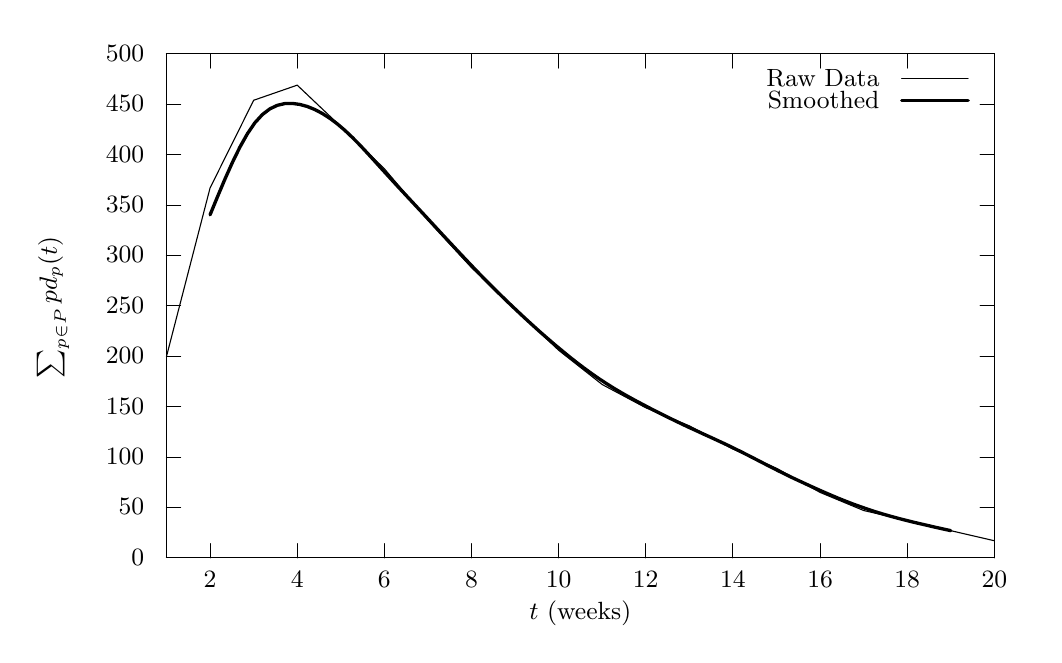
\begin{tikzpicture}[gnuplot]
%% generated with GNUPLOT 4.6p4 (Lua 5.1; terminal rev. 99, script rev. 100)
%% Thu 04 Sep 2014 10:50:27 WST
\tikzset{every node/.append style={font={\fontsize{9pt}{10.8pt}\selectfont}}}
\gpmonochromelines
\path (0.000,0.000) rectangle (12.700,7.620);
\gpcolor{color=gp lt color border}
\gpsetlinetype{gp lt border}
\gpsetlinewidth{1.00}
\draw[gp path] (1.688,0.886)--(1.868,0.886);
\draw[gp path] (12.201,0.886)--(12.021,0.886);
\node[gp node right] at (1.522,0.886) { 0};
\draw[gp path] (1.688,1.526)--(1.868,1.526);
\draw[gp path] (12.201,1.526)--(12.021,1.526);
\node[gp node right] at (1.522,1.526) { 50};
\draw[gp path] (1.688,2.166)--(1.868,2.166);
\draw[gp path] (12.201,2.166)--(12.021,2.166);
\node[gp node right] at (1.522,2.166) { 100};
\draw[gp path] (1.688,2.806)--(1.868,2.806);
\draw[gp path] (12.201,2.806)--(12.021,2.806);
\node[gp node right] at (1.522,2.806) { 150};
\draw[gp path] (1.688,3.446)--(1.868,3.446);
\draw[gp path] (12.201,3.446)--(12.021,3.446);
\node[gp node right] at (1.522,3.446) { 200};
\draw[gp path] (1.688,4.087)--(1.868,4.087);
\draw[gp path] (12.201,4.087)--(12.021,4.087);
\node[gp node right] at (1.522,4.087) { 250};
\draw[gp path] (1.688,4.727)--(1.868,4.727);
\draw[gp path] (12.201,4.727)--(12.021,4.727);
\node[gp node right] at (1.522,4.727) { 300};
\draw[gp path] (1.688,5.367)--(1.868,5.367);
\draw[gp path] (12.201,5.367)--(12.021,5.367);
\node[gp node right] at (1.522,5.367) { 350};
\draw[gp path] (1.688,6.007)--(1.868,6.007);
\draw[gp path] (12.201,6.007)--(12.021,6.007);
\node[gp node right] at (1.522,6.007) { 400};
\draw[gp path] (1.688,6.647)--(1.868,6.647);
\draw[gp path] (12.201,6.647)--(12.021,6.647);
\node[gp node right] at (1.522,6.647) { 450};
\draw[gp path] (1.688,7.287)--(1.868,7.287);
\draw[gp path] (12.201,7.287)--(12.021,7.287);
\node[gp node right] at (1.522,7.287) { 500};
\draw[gp path] (2.241,0.886)--(2.241,1.066);
\draw[gp path] (2.241,7.287)--(2.241,7.107);
\node[gp node center] at (2.241,0.609) { 2};
\draw[gp path] (3.348,0.886)--(3.348,1.066);
\draw[gp path] (3.348,7.287)--(3.348,7.107);
\node[gp node center] at (3.348,0.609) { 4};
\draw[gp path] (4.455,0.886)--(4.455,1.066);
\draw[gp path] (4.455,7.287)--(4.455,7.107);
\node[gp node center] at (4.455,0.609) { 6};
\draw[gp path] (5.561,0.886)--(5.561,1.066);
\draw[gp path] (5.561,7.287)--(5.561,7.107);
\node[gp node center] at (5.561,0.609) { 8};
\draw[gp path] (6.668,0.886)--(6.668,1.066);
\draw[gp path] (6.668,7.287)--(6.668,7.107);
\node[gp node center] at (6.668,0.609) { 10};
\draw[gp path] (7.774,0.886)--(7.774,1.066);
\draw[gp path] (7.774,7.287)--(7.774,7.107);
\node[gp node center] at (7.774,0.609) { 12};
\draw[gp path] (8.881,0.886)--(8.881,1.066);
\draw[gp path] (8.881,7.287)--(8.881,7.107);
\node[gp node center] at (8.881,0.609) { 14};
\draw[gp path] (9.988,0.886)--(9.988,1.066);
\draw[gp path] (9.988,7.287)--(9.988,7.107);
\node[gp node center] at (9.988,0.609) { 16};
\draw[gp path] (11.094,0.886)--(11.094,1.066);
\draw[gp path] (11.094,7.287)--(11.094,7.107);
\node[gp node center] at (11.094,0.609) { 18};
\draw[gp path] (12.201,0.886)--(12.201,1.066);
\draw[gp path] (12.201,7.287)--(12.201,7.107);
\node[gp node center] at (12.201,0.609) { 20};
\draw[gp path] (1.688,7.287)--(1.688,0.886)--(12.201,0.886)--(12.201,7.287)--cycle;
\node[gp node center,rotate=-270] at (0.221,4.086) {$\sum_{p \in P} p d_p(t)$};
\node[gp node center] at (6.944,0.194) {$t$ (weeks)};
\node[gp node right] at (10.859,6.969) {Raw Data};
\gpcolor{color=gp lt color 3}
\gpsetlinetype{gp lt plot 3}
\draw[gp path] (11.025,6.969)--(11.869,6.969);
\draw[gp path] (1.688,3.446)--(2.241,5.584)--(2.795,6.698)--(3.348,6.890)--(3.901,6.365)%
  --(4.455,5.828)--(5.008,5.175)--(5.561,4.573)--(6.115,4.048)--(6.668,3.523)--(7.221,3.088)%
  --(7.774,2.793)--(8.328,2.563)--(8.881,2.269)--(9.434,2.025)--(9.988,1.718)--(10.541,1.488)%
  --(11.094,1.360)--(11.648,1.232)--(12.201,1.104);
\gpcolor{color=gp lt color border}
\node[gp node right] at (10.859,6.692) {Smoothed};
\gpcolor{color=gp lt color 0}
\gpsetlinetype{gp lt plot 0}
\gpsetlinewidth{3.00}
\draw[gp path] (11.025,6.692)--(11.869,6.692);
\draw[gp path] (2.241,5.243)--(2.336,5.474)--(2.431,5.699)--(2.526,5.911)--(2.621,6.105)%
  --(2.716,6.274)--(2.811,6.413)--(2.906,6.517)--(3.001,6.589)--(3.096,6.634)--(3.191,6.656)%
  --(3.286,6.658)--(3.381,6.645)--(3.476,6.619)--(3.572,6.580)--(3.667,6.530)--(3.762,6.469)%
  --(3.857,6.398)--(3.952,6.317)--(4.047,6.227)--(4.142,6.131)--(4.237,6.029)--(4.332,5.925)%
  --(4.427,5.820)--(4.522,5.716)--(4.617,5.612)--(4.712,5.510)--(4.807,5.408)--(4.902,5.306)%
  --(4.997,5.204)--(5.092,5.101)--(5.187,4.998)--(5.282,4.896)--(5.377,4.794)--(5.472,4.693)%
  --(5.567,4.593)--(5.662,4.494)--(5.757,4.398)--(5.852,4.303)--(5.947,4.209)--(6.042,4.117)%
  --(6.137,4.027)--(6.232,3.938)--(6.327,3.851)--(6.422,3.765)--(6.517,3.682)--(6.612,3.600)%
  --(6.707,3.521)--(6.802,3.443)--(6.897,3.368)--(6.992,3.296)--(7.087,3.227)--(7.182,3.161)%
  --(7.277,3.099)--(7.372,3.039)--(7.467,2.983)--(7.562,2.929)--(7.657,2.877)--(7.752,2.827)%
  --(7.847,2.777)--(7.942,2.729)--(8.037,2.681)--(8.132,2.635)--(8.227,2.589)--(8.322,2.544)%
  --(8.417,2.501)--(8.512,2.457)--(8.607,2.414)--(8.702,2.370)--(8.797,2.326)--(8.892,2.280)%
  --(8.987,2.233)--(9.082,2.185)--(9.177,2.136)--(9.272,2.087)--(9.367,2.038)--(9.462,1.990)%
  --(9.557,1.943)--(9.652,1.897)--(9.747,1.853)--(9.842,1.809)--(9.937,1.766)--(10.032,1.724)%
  --(10.127,1.683)--(10.222,1.643)--(10.317,1.605)--(10.413,1.568)--(10.508,1.534)--(10.603,1.501)%
  --(10.698,1.470)--(10.793,1.441)--(10.888,1.414)--(10.983,1.388)--(11.078,1.364)--(11.173,1.340)%
  --(11.268,1.318)--(11.363,1.296)--(11.458,1.274)--(11.553,1.253)--(11.648,1.232);
\gpcolor{color=gp lt color border}
\gpsetlinetype{gp lt border}
\gpsetlinewidth{1.00}
\draw[gp path] (1.688,7.287)--(1.688,0.886)--(12.201,0.886)--(12.201,7.287)--cycle;
%% coordinates of the plot area
\gpdefrectangularnode{gp plot 1}{\pgfpoint{1.688cm}{0.886cm}}{\pgfpoint{12.201cm}{7.287cm}}
\end{tikzpicture}
%% gnuplot variables

    \caption{Scenario D Result}
  \end{figure}
 
  
  \clearpage
  \subsection{Average queue time of major defects still to be fixed}
  \begin{figure}[!htb]
    \centering
    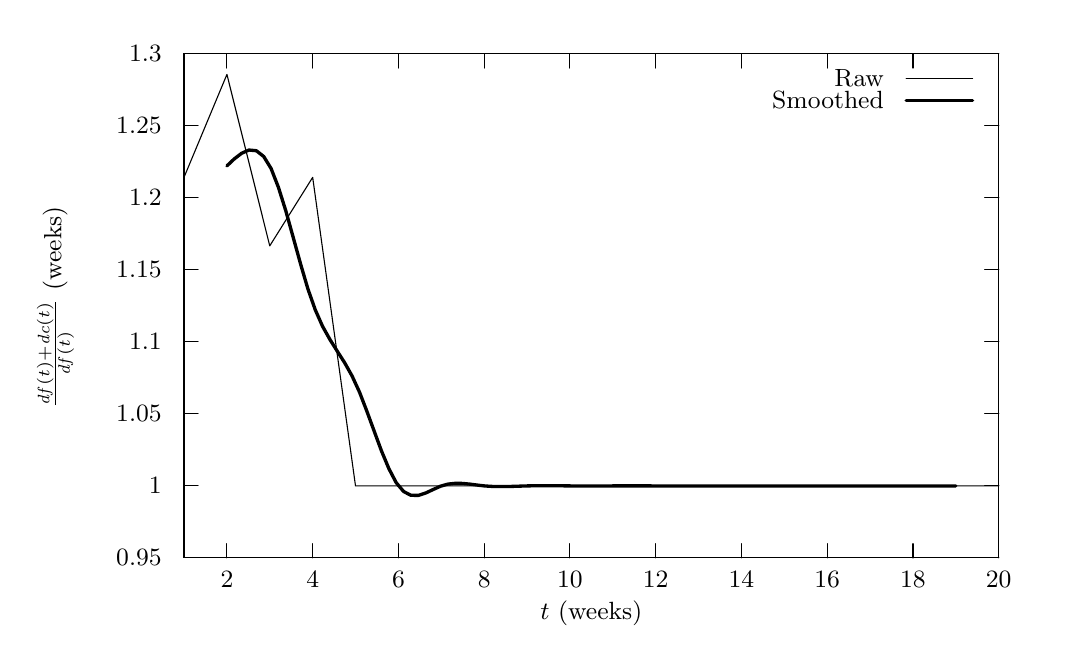
\begin{tikzpicture}[gnuplot]
%% generated with GNUPLOT 4.6p5 (Lua 5.2; terminal rev. 99, script rev. 100)
%% 2/09/2014 2:44:57 PM
\tikzset{every node/.append style={font={\fontsize{9pt}{10.8pt}\selectfont}}}
\gpmonochromelines
\path (0.000,0.000) rectangle (12.700,7.620);
\gpcolor{color=gp lt color border}
\gpsetlinetype{gp lt border}
\gpsetlinewidth{1.00}
\draw[gp path] (1.854,0.886)--(2.034,0.886);
\draw[gp path] (12.201,0.886)--(12.021,0.886);
\node[gp node right] at (1.688,0.886) { 0.95};
\draw[gp path] (1.854,1.800)--(2.034,1.800);
\draw[gp path] (12.201,1.800)--(12.021,1.800);
\node[gp node right] at (1.688,1.800) { 1};
\draw[gp path] (1.854,2.715)--(2.034,2.715);
\draw[gp path] (12.201,2.715)--(12.021,2.715);
\node[gp node right] at (1.688,2.715) { 1.05};
\draw[gp path] (1.854,3.629)--(2.034,3.629);
\draw[gp path] (12.201,3.629)--(12.021,3.629);
\node[gp node right] at (1.688,3.629) { 1.1};
\draw[gp path] (1.854,4.544)--(2.034,4.544);
\draw[gp path] (12.201,4.544)--(12.021,4.544);
\node[gp node right] at (1.688,4.544) { 1.15};
\draw[gp path] (1.854,5.458)--(2.034,5.458);
\draw[gp path] (12.201,5.458)--(12.021,5.458);
\node[gp node right] at (1.688,5.458) { 1.2};
\draw[gp path] (1.854,6.373)--(2.034,6.373);
\draw[gp path] (12.201,6.373)--(12.021,6.373);
\node[gp node right] at (1.688,6.373) { 1.25};
\draw[gp path] (1.854,7.287)--(2.034,7.287);
\draw[gp path] (12.201,7.287)--(12.021,7.287);
\node[gp node right] at (1.688,7.287) { 1.3};
\draw[gp path] (2.399,0.886)--(2.399,1.066);
\draw[gp path] (2.399,7.287)--(2.399,7.107);
\node[gp node center] at (2.399,0.609) { 2};
\draw[gp path] (3.488,0.886)--(3.488,1.066);
\draw[gp path] (3.488,7.287)--(3.488,7.107);
\node[gp node center] at (3.488,0.609) { 4};
\draw[gp path] (4.577,0.886)--(4.577,1.066);
\draw[gp path] (4.577,7.287)--(4.577,7.107);
\node[gp node center] at (4.577,0.609) { 6};
\draw[gp path] (5.666,0.886)--(5.666,1.066);
\draw[gp path] (5.666,7.287)--(5.666,7.107);
\node[gp node center] at (5.666,0.609) { 8};
\draw[gp path] (6.755,0.886)--(6.755,1.066);
\draw[gp path] (6.755,7.287)--(6.755,7.107);
\node[gp node center] at (6.755,0.609) { 10};
\draw[gp path] (7.844,0.886)--(7.844,1.066);
\draw[gp path] (7.844,7.287)--(7.844,7.107);
\node[gp node center] at (7.844,0.609) { 12};
\draw[gp path] (8.934,0.886)--(8.934,1.066);
\draw[gp path] (8.934,7.287)--(8.934,7.107);
\node[gp node center] at (8.934,0.609) { 14};
\draw[gp path] (10.023,0.886)--(10.023,1.066);
\draw[gp path] (10.023,7.287)--(10.023,7.107);
\node[gp node center] at (10.023,0.609) { 16};
\draw[gp path] (11.112,0.886)--(11.112,1.066);
\draw[gp path] (11.112,7.287)--(11.112,7.107);
\node[gp node center] at (11.112,0.609) { 18};
\draw[gp path] (12.201,0.886)--(12.201,1.066);
\draw[gp path] (12.201,7.287)--(12.201,7.107);
\node[gp node center] at (12.201,0.609) { 20};
\draw[gp path] (1.854,7.287)--(1.854,0.886)--(12.201,0.886)--(12.201,7.287)--cycle;
\node[gp node center,rotate=-270] at (0.221,4.086) {$\frac{\mathit{df}(t) + \mathit{dc}(t)}{\mathit{df}(t)}$ (weeks)};
\node[gp node center] at (7.027,0.194) {$t$ (weeks)};
\node[gp node right] at (10.859,6.969) {Raw};
\gpcolor{color=gp lt color 3}
\gpsetlinetype{gp lt plot 3}
\draw[gp path] (11.025,6.969)--(11.869,6.969);
\draw[gp path] (1.854,5.719)--(2.399,7.026)--(2.943,4.849)--(3.488,5.719)--(4.032,1.800)%
  --(4.577,1.800)--(5.121,1.800)--(5.666,1.800)--(6.211,1.800)--(6.755,1.800)--(7.300,1.800)%
  --(7.844,1.800)--(8.389,1.800)--(8.934,1.800)--(9.478,1.800)--(10.023,1.800)--(10.567,1.800)%
  --(11.656,1.800)--(12.201,1.800);
\gpcolor{color=gp lt color border}
\node[gp node right] at (10.859,6.692) {Smoothed};
\gpcolor{color=gp lt color 0}
\gpsetlinetype{gp lt plot 0}
\gpsetlinewidth{3.00}
\draw[gp path] (11.025,6.692)--(11.869,6.692);
\draw[gp path] (2.399,5.865)--(2.492,5.953)--(2.586,6.025)--(2.679,6.066)--(2.773,6.057)%
  --(2.866,5.984)--(2.960,5.831)--(3.053,5.592)--(3.147,5.293)--(3.240,4.959)--(3.334,4.620)%
  --(3.427,4.303)--(3.521,4.036)--(3.614,3.826)--(3.708,3.658)--(3.801,3.510)--(3.895,3.363)%
  --(3.988,3.197)--(4.082,2.993)--(4.175,2.752)--(4.269,2.496)--(4.362,2.244)--(4.456,2.019)%
  --(4.549,1.841)--(4.643,1.729)--(4.736,1.681)--(4.830,1.680)--(4.923,1.710)--(5.017,1.754)%
  --(5.110,1.796)--(5.204,1.823)--(5.297,1.833)--(5.391,1.832)--(5.485,1.823)--(5.578,1.811)%
  --(5.672,1.800)--(5.765,1.794)--(5.859,1.792)--(5.952,1.792)--(6.046,1.795)--(6.139,1.798)%
  --(6.233,1.801)--(6.326,1.802)--(6.420,1.803)--(6.513,1.802)--(6.607,1.802)--(6.700,1.801)%
  --(6.794,1.800)--(6.887,1.800)--(6.981,1.800)--(7.074,1.800)--(7.168,1.800)--(7.261,1.800)%
  --(7.355,1.801)--(7.448,1.801)--(7.542,1.801)--(7.635,1.801)--(7.729,1.801)--(7.822,1.800)%
  --(7.916,1.800)--(8.009,1.800)--(8.103,1.800)--(8.196,1.800)--(8.290,1.800)--(8.383,1.800)%
  --(8.477,1.800)--(8.570,1.800)--(8.664,1.800)--(8.758,1.800)--(8.851,1.800)--(8.945,1.800)%
  --(9.038,1.800)--(9.132,1.800)--(9.225,1.800)--(9.319,1.800)--(9.412,1.800)--(9.506,1.800)%
  --(9.599,1.800)--(9.693,1.800)--(9.786,1.800)--(9.880,1.800)--(9.973,1.800)--(10.067,1.800)%
  --(10.160,1.800)--(10.254,1.800)--(10.347,1.800)--(10.441,1.800)--(10.534,1.800)--(10.628,1.800)%
  --(10.721,1.800)--(10.815,1.800)--(10.908,1.800)--(11.002,1.800)--(11.095,1.800)--(11.189,1.800)%
  --(11.282,1.800)--(11.376,1.800)--(11.469,1.800)--(11.563,1.800)--(11.656,1.800);
\gpcolor{color=gp lt color border}
\gpsetlinetype{gp lt border}
\gpsetlinewidth{1.00}
\draw[gp path] (1.854,7.287)--(1.854,0.886)--(12.201,0.886)--(12.201,7.287)--cycle;
%% coordinates of the plot area
\gpdefrectangularnode{gp plot 1}{\pgfpoint{1.854cm}{0.886cm}}{\pgfpoint{12.201cm}{7.287cm}}
\end{tikzpicture}
%% gnuplot variables

    \caption{Scenario B Result}
  \end{figure}
  
  \begin{figure}[!htb]
    \centering
    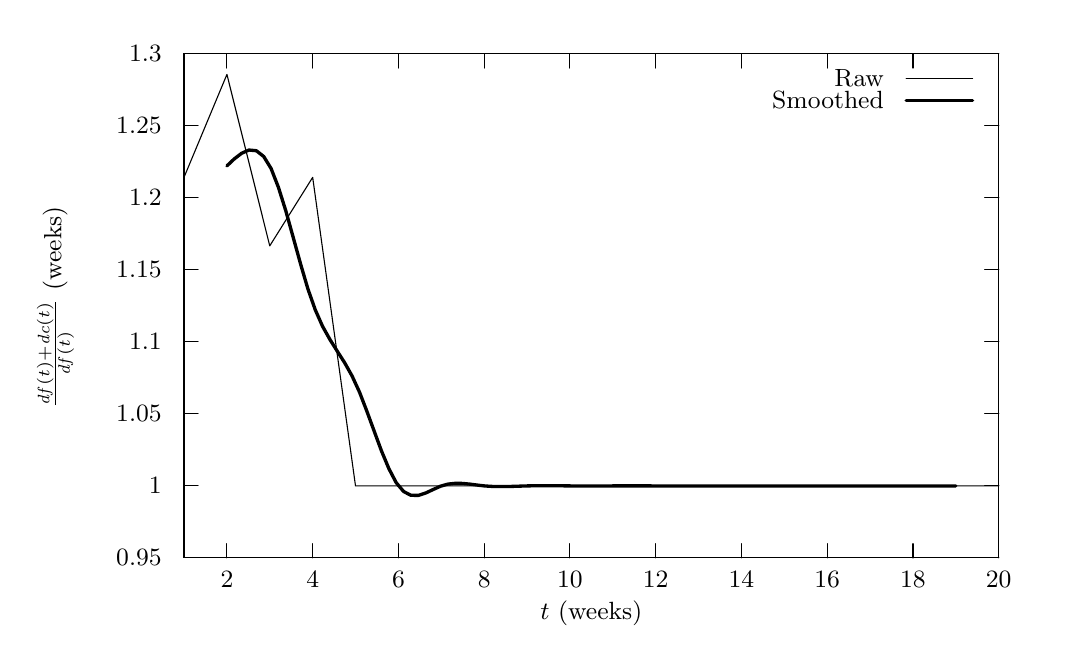
\begin{tikzpicture}[gnuplot]
%% generated with GNUPLOT 4.6p5 (Lua 5.2; terminal rev. 99, script rev. 100)
%% 2/09/2014 2:44:57 PM
\tikzset{every node/.append style={font={\fontsize{9pt}{10.8pt}\selectfont}}}
\gpmonochromelines
\path (0.000,0.000) rectangle (12.700,7.620);
\gpcolor{color=gp lt color border}
\gpsetlinetype{gp lt border}
\gpsetlinewidth{1.00}
\draw[gp path] (1.854,0.886)--(2.034,0.886);
\draw[gp path] (12.201,0.886)--(12.021,0.886);
\node[gp node right] at (1.688,0.886) { 0.95};
\draw[gp path] (1.854,1.800)--(2.034,1.800);
\draw[gp path] (12.201,1.800)--(12.021,1.800);
\node[gp node right] at (1.688,1.800) { 1};
\draw[gp path] (1.854,2.715)--(2.034,2.715);
\draw[gp path] (12.201,2.715)--(12.021,2.715);
\node[gp node right] at (1.688,2.715) { 1.05};
\draw[gp path] (1.854,3.629)--(2.034,3.629);
\draw[gp path] (12.201,3.629)--(12.021,3.629);
\node[gp node right] at (1.688,3.629) { 1.1};
\draw[gp path] (1.854,4.544)--(2.034,4.544);
\draw[gp path] (12.201,4.544)--(12.021,4.544);
\node[gp node right] at (1.688,4.544) { 1.15};
\draw[gp path] (1.854,5.458)--(2.034,5.458);
\draw[gp path] (12.201,5.458)--(12.021,5.458);
\node[gp node right] at (1.688,5.458) { 1.2};
\draw[gp path] (1.854,6.373)--(2.034,6.373);
\draw[gp path] (12.201,6.373)--(12.021,6.373);
\node[gp node right] at (1.688,6.373) { 1.25};
\draw[gp path] (1.854,7.287)--(2.034,7.287);
\draw[gp path] (12.201,7.287)--(12.021,7.287);
\node[gp node right] at (1.688,7.287) { 1.3};
\draw[gp path] (2.399,0.886)--(2.399,1.066);
\draw[gp path] (2.399,7.287)--(2.399,7.107);
\node[gp node center] at (2.399,0.609) { 2};
\draw[gp path] (3.488,0.886)--(3.488,1.066);
\draw[gp path] (3.488,7.287)--(3.488,7.107);
\node[gp node center] at (3.488,0.609) { 4};
\draw[gp path] (4.577,0.886)--(4.577,1.066);
\draw[gp path] (4.577,7.287)--(4.577,7.107);
\node[gp node center] at (4.577,0.609) { 6};
\draw[gp path] (5.666,0.886)--(5.666,1.066);
\draw[gp path] (5.666,7.287)--(5.666,7.107);
\node[gp node center] at (5.666,0.609) { 8};
\draw[gp path] (6.755,0.886)--(6.755,1.066);
\draw[gp path] (6.755,7.287)--(6.755,7.107);
\node[gp node center] at (6.755,0.609) { 10};
\draw[gp path] (7.844,0.886)--(7.844,1.066);
\draw[gp path] (7.844,7.287)--(7.844,7.107);
\node[gp node center] at (7.844,0.609) { 12};
\draw[gp path] (8.934,0.886)--(8.934,1.066);
\draw[gp path] (8.934,7.287)--(8.934,7.107);
\node[gp node center] at (8.934,0.609) { 14};
\draw[gp path] (10.023,0.886)--(10.023,1.066);
\draw[gp path] (10.023,7.287)--(10.023,7.107);
\node[gp node center] at (10.023,0.609) { 16};
\draw[gp path] (11.112,0.886)--(11.112,1.066);
\draw[gp path] (11.112,7.287)--(11.112,7.107);
\node[gp node center] at (11.112,0.609) { 18};
\draw[gp path] (12.201,0.886)--(12.201,1.066);
\draw[gp path] (12.201,7.287)--(12.201,7.107);
\node[gp node center] at (12.201,0.609) { 20};
\draw[gp path] (1.854,7.287)--(1.854,0.886)--(12.201,0.886)--(12.201,7.287)--cycle;
\node[gp node center,rotate=-270] at (0.221,4.086) {$\frac{\mathit{df}(t) + \mathit{dc}(t)}{\mathit{df}(t)}$ (weeks)};
\node[gp node center] at (7.027,0.194) {$t$ (weeks)};
\node[gp node right] at (10.859,6.969) {Raw};
\gpcolor{color=gp lt color 3}
\gpsetlinetype{gp lt plot 3}
\draw[gp path] (11.025,6.969)--(11.869,6.969);
\draw[gp path] (1.854,5.719)--(2.399,7.026)--(2.943,4.849)--(3.488,5.719)--(4.032,1.800)%
  --(4.577,1.800)--(5.121,1.800)--(5.666,1.800)--(6.211,1.800)--(6.755,1.800)--(7.300,1.800)%
  --(7.844,1.800)--(8.389,1.800)--(8.934,1.800)--(9.478,1.800)--(10.023,1.800)--(10.567,1.800)%
  --(11.656,1.800)--(12.201,1.800);
\gpcolor{color=gp lt color border}
\node[gp node right] at (10.859,6.692) {Smoothed};
\gpcolor{color=gp lt color 0}
\gpsetlinetype{gp lt plot 0}
\gpsetlinewidth{3.00}
\draw[gp path] (11.025,6.692)--(11.869,6.692);
\draw[gp path] (2.399,5.865)--(2.492,5.953)--(2.586,6.025)--(2.679,6.066)--(2.773,6.057)%
  --(2.866,5.984)--(2.960,5.831)--(3.053,5.592)--(3.147,5.293)--(3.240,4.959)--(3.334,4.620)%
  --(3.427,4.303)--(3.521,4.036)--(3.614,3.826)--(3.708,3.658)--(3.801,3.510)--(3.895,3.363)%
  --(3.988,3.197)--(4.082,2.993)--(4.175,2.752)--(4.269,2.496)--(4.362,2.244)--(4.456,2.019)%
  --(4.549,1.841)--(4.643,1.729)--(4.736,1.681)--(4.830,1.680)--(4.923,1.710)--(5.017,1.754)%
  --(5.110,1.796)--(5.204,1.823)--(5.297,1.833)--(5.391,1.832)--(5.485,1.823)--(5.578,1.811)%
  --(5.672,1.800)--(5.765,1.794)--(5.859,1.792)--(5.952,1.792)--(6.046,1.795)--(6.139,1.798)%
  --(6.233,1.801)--(6.326,1.802)--(6.420,1.803)--(6.513,1.802)--(6.607,1.802)--(6.700,1.801)%
  --(6.794,1.800)--(6.887,1.800)--(6.981,1.800)--(7.074,1.800)--(7.168,1.800)--(7.261,1.800)%
  --(7.355,1.801)--(7.448,1.801)--(7.542,1.801)--(7.635,1.801)--(7.729,1.801)--(7.822,1.800)%
  --(7.916,1.800)--(8.009,1.800)--(8.103,1.800)--(8.196,1.800)--(8.290,1.800)--(8.383,1.800)%
  --(8.477,1.800)--(8.570,1.800)--(8.664,1.800)--(8.758,1.800)--(8.851,1.800)--(8.945,1.800)%
  --(9.038,1.800)--(9.132,1.800)--(9.225,1.800)--(9.319,1.800)--(9.412,1.800)--(9.506,1.800)%
  --(9.599,1.800)--(9.693,1.800)--(9.786,1.800)--(9.880,1.800)--(9.973,1.800)--(10.067,1.800)%
  --(10.160,1.800)--(10.254,1.800)--(10.347,1.800)--(10.441,1.800)--(10.534,1.800)--(10.628,1.800)%
  --(10.721,1.800)--(10.815,1.800)--(10.908,1.800)--(11.002,1.800)--(11.095,1.800)--(11.189,1.800)%
  --(11.282,1.800)--(11.376,1.800)--(11.469,1.800)--(11.563,1.800)--(11.656,1.800);
\gpcolor{color=gp lt color border}
\gpsetlinetype{gp lt border}
\gpsetlinewidth{1.00}
\draw[gp path] (1.854,7.287)--(1.854,0.886)--(12.201,0.886)--(12.201,7.287)--cycle;
%% coordinates of the plot area
\gpdefrectangularnode{gp plot 1}{\pgfpoint{1.854cm}{0.886cm}}{\pgfpoint{12.201cm}{7.287cm}}
\end{tikzpicture}
%% gnuplot variables

    \caption{Scenario C Result}
  \end{figure}
  
  \begin{figure}[!htb]
    \centering
    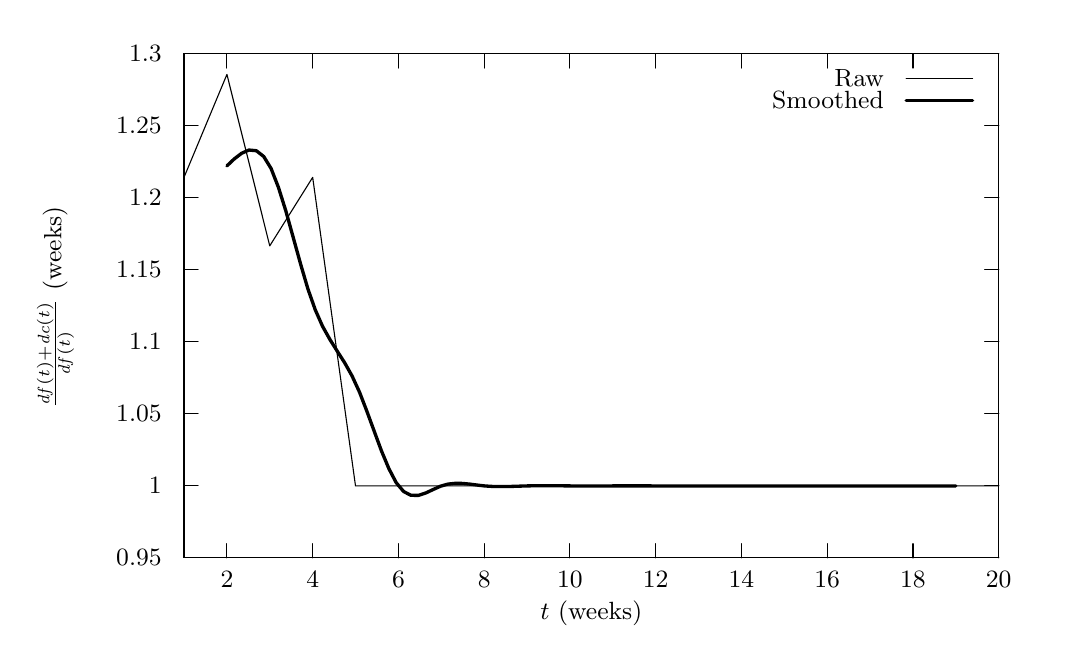
\begin{tikzpicture}[gnuplot]
%% generated with GNUPLOT 4.6p5 (Lua 5.2; terminal rev. 99, script rev. 100)
%% 2/09/2014 2:44:57 PM
\tikzset{every node/.append style={font={\fontsize{9pt}{10.8pt}\selectfont}}}
\gpmonochromelines
\path (0.000,0.000) rectangle (12.700,7.620);
\gpcolor{color=gp lt color border}
\gpsetlinetype{gp lt border}
\gpsetlinewidth{1.00}
\draw[gp path] (1.854,0.886)--(2.034,0.886);
\draw[gp path] (12.201,0.886)--(12.021,0.886);
\node[gp node right] at (1.688,0.886) { 0.95};
\draw[gp path] (1.854,1.800)--(2.034,1.800);
\draw[gp path] (12.201,1.800)--(12.021,1.800);
\node[gp node right] at (1.688,1.800) { 1};
\draw[gp path] (1.854,2.715)--(2.034,2.715);
\draw[gp path] (12.201,2.715)--(12.021,2.715);
\node[gp node right] at (1.688,2.715) { 1.05};
\draw[gp path] (1.854,3.629)--(2.034,3.629);
\draw[gp path] (12.201,3.629)--(12.021,3.629);
\node[gp node right] at (1.688,3.629) { 1.1};
\draw[gp path] (1.854,4.544)--(2.034,4.544);
\draw[gp path] (12.201,4.544)--(12.021,4.544);
\node[gp node right] at (1.688,4.544) { 1.15};
\draw[gp path] (1.854,5.458)--(2.034,5.458);
\draw[gp path] (12.201,5.458)--(12.021,5.458);
\node[gp node right] at (1.688,5.458) { 1.2};
\draw[gp path] (1.854,6.373)--(2.034,6.373);
\draw[gp path] (12.201,6.373)--(12.021,6.373);
\node[gp node right] at (1.688,6.373) { 1.25};
\draw[gp path] (1.854,7.287)--(2.034,7.287);
\draw[gp path] (12.201,7.287)--(12.021,7.287);
\node[gp node right] at (1.688,7.287) { 1.3};
\draw[gp path] (2.399,0.886)--(2.399,1.066);
\draw[gp path] (2.399,7.287)--(2.399,7.107);
\node[gp node center] at (2.399,0.609) { 2};
\draw[gp path] (3.488,0.886)--(3.488,1.066);
\draw[gp path] (3.488,7.287)--(3.488,7.107);
\node[gp node center] at (3.488,0.609) { 4};
\draw[gp path] (4.577,0.886)--(4.577,1.066);
\draw[gp path] (4.577,7.287)--(4.577,7.107);
\node[gp node center] at (4.577,0.609) { 6};
\draw[gp path] (5.666,0.886)--(5.666,1.066);
\draw[gp path] (5.666,7.287)--(5.666,7.107);
\node[gp node center] at (5.666,0.609) { 8};
\draw[gp path] (6.755,0.886)--(6.755,1.066);
\draw[gp path] (6.755,7.287)--(6.755,7.107);
\node[gp node center] at (6.755,0.609) { 10};
\draw[gp path] (7.844,0.886)--(7.844,1.066);
\draw[gp path] (7.844,7.287)--(7.844,7.107);
\node[gp node center] at (7.844,0.609) { 12};
\draw[gp path] (8.934,0.886)--(8.934,1.066);
\draw[gp path] (8.934,7.287)--(8.934,7.107);
\node[gp node center] at (8.934,0.609) { 14};
\draw[gp path] (10.023,0.886)--(10.023,1.066);
\draw[gp path] (10.023,7.287)--(10.023,7.107);
\node[gp node center] at (10.023,0.609) { 16};
\draw[gp path] (11.112,0.886)--(11.112,1.066);
\draw[gp path] (11.112,7.287)--(11.112,7.107);
\node[gp node center] at (11.112,0.609) { 18};
\draw[gp path] (12.201,0.886)--(12.201,1.066);
\draw[gp path] (12.201,7.287)--(12.201,7.107);
\node[gp node center] at (12.201,0.609) { 20};
\draw[gp path] (1.854,7.287)--(1.854,0.886)--(12.201,0.886)--(12.201,7.287)--cycle;
\node[gp node center,rotate=-270] at (0.221,4.086) {$\frac{\mathit{df}(t) + \mathit{dc}(t)}{\mathit{df}(t)}$ (weeks)};
\node[gp node center] at (7.027,0.194) {$t$ (weeks)};
\node[gp node right] at (10.859,6.969) {Raw};
\gpcolor{color=gp lt color 3}
\gpsetlinetype{gp lt plot 3}
\draw[gp path] (11.025,6.969)--(11.869,6.969);
\draw[gp path] (1.854,5.719)--(2.399,7.026)--(2.943,4.849)--(3.488,5.719)--(4.032,1.800)%
  --(4.577,1.800)--(5.121,1.800)--(5.666,1.800)--(6.211,1.800)--(6.755,1.800)--(7.300,1.800)%
  --(7.844,1.800)--(8.389,1.800)--(8.934,1.800)--(9.478,1.800)--(10.023,1.800)--(10.567,1.800)%
  --(11.656,1.800)--(12.201,1.800);
\gpcolor{color=gp lt color border}
\node[gp node right] at (10.859,6.692) {Smoothed};
\gpcolor{color=gp lt color 0}
\gpsetlinetype{gp lt plot 0}
\gpsetlinewidth{3.00}
\draw[gp path] (11.025,6.692)--(11.869,6.692);
\draw[gp path] (2.399,5.865)--(2.492,5.953)--(2.586,6.025)--(2.679,6.066)--(2.773,6.057)%
  --(2.866,5.984)--(2.960,5.831)--(3.053,5.592)--(3.147,5.293)--(3.240,4.959)--(3.334,4.620)%
  --(3.427,4.303)--(3.521,4.036)--(3.614,3.826)--(3.708,3.658)--(3.801,3.510)--(3.895,3.363)%
  --(3.988,3.197)--(4.082,2.993)--(4.175,2.752)--(4.269,2.496)--(4.362,2.244)--(4.456,2.019)%
  --(4.549,1.841)--(4.643,1.729)--(4.736,1.681)--(4.830,1.680)--(4.923,1.710)--(5.017,1.754)%
  --(5.110,1.796)--(5.204,1.823)--(5.297,1.833)--(5.391,1.832)--(5.485,1.823)--(5.578,1.811)%
  --(5.672,1.800)--(5.765,1.794)--(5.859,1.792)--(5.952,1.792)--(6.046,1.795)--(6.139,1.798)%
  --(6.233,1.801)--(6.326,1.802)--(6.420,1.803)--(6.513,1.802)--(6.607,1.802)--(6.700,1.801)%
  --(6.794,1.800)--(6.887,1.800)--(6.981,1.800)--(7.074,1.800)--(7.168,1.800)--(7.261,1.800)%
  --(7.355,1.801)--(7.448,1.801)--(7.542,1.801)--(7.635,1.801)--(7.729,1.801)--(7.822,1.800)%
  --(7.916,1.800)--(8.009,1.800)--(8.103,1.800)--(8.196,1.800)--(8.290,1.800)--(8.383,1.800)%
  --(8.477,1.800)--(8.570,1.800)--(8.664,1.800)--(8.758,1.800)--(8.851,1.800)--(8.945,1.800)%
  --(9.038,1.800)--(9.132,1.800)--(9.225,1.800)--(9.319,1.800)--(9.412,1.800)--(9.506,1.800)%
  --(9.599,1.800)--(9.693,1.800)--(9.786,1.800)--(9.880,1.800)--(9.973,1.800)--(10.067,1.800)%
  --(10.160,1.800)--(10.254,1.800)--(10.347,1.800)--(10.441,1.800)--(10.534,1.800)--(10.628,1.800)%
  --(10.721,1.800)--(10.815,1.800)--(10.908,1.800)--(11.002,1.800)--(11.095,1.800)--(11.189,1.800)%
  --(11.282,1.800)--(11.376,1.800)--(11.469,1.800)--(11.563,1.800)--(11.656,1.800);
\gpcolor{color=gp lt color border}
\gpsetlinetype{gp lt border}
\gpsetlinewidth{1.00}
\draw[gp path] (1.854,7.287)--(1.854,0.886)--(12.201,0.886)--(12.201,7.287)--cycle;
%% coordinates of the plot area
\gpdefrectangularnode{gp plot 1}{\pgfpoint{1.854cm}{0.886cm}}{\pgfpoint{12.201cm}{7.287cm}}
\end{tikzpicture}
%% gnuplot variables

    \caption{Scenario D Result}
  \end{figure}
  
  \clearpage
  \subsection{Estimate of number of unfixed defects still in software}
  \begin{figure}[!htb]
    \centering
    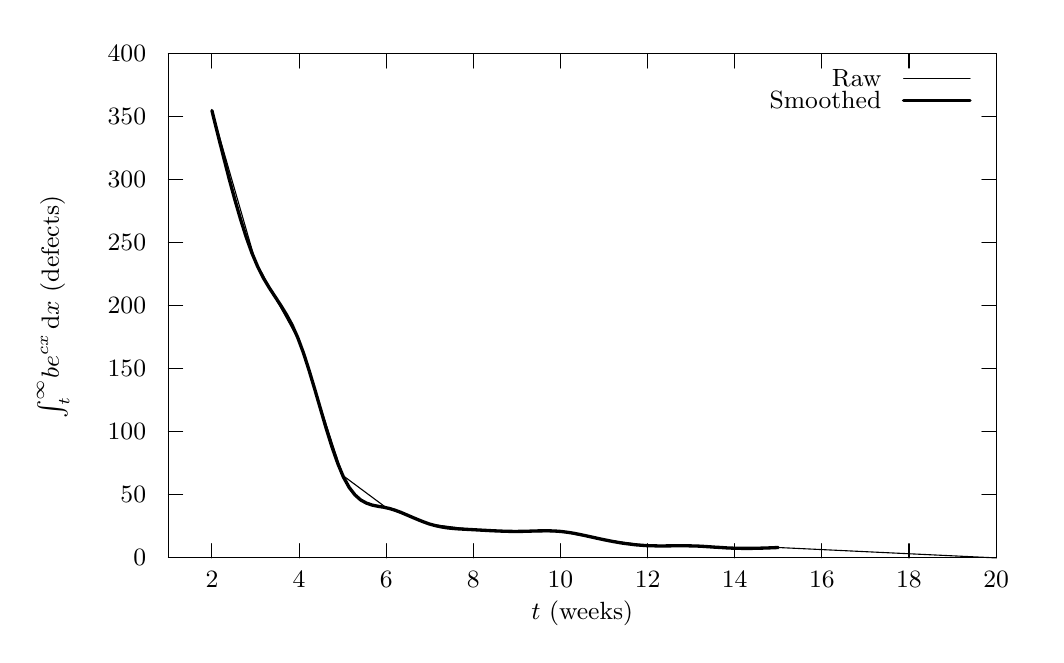
\begin{tikzpicture}[gnuplot]
%% generated with GNUPLOT 4.6p4 (Lua 5.1; terminal rev. 99, script rev. 100)
%% Thu 04 Sep 2014 10:50:27 WST
\tikzset{every node/.append style={font={\fontsize{9pt}{10.8pt}\selectfont}}}
\gpmonochromelines
\path (0.000,0.000) rectangle (12.700,7.620);
\gpcolor{color=gp lt color border}
\gpsetlinetype{gp lt border}
\gpsetlinewidth{1.00}
\draw[gp path] (1.688,0.886)--(1.868,0.886);
\draw[gp path] (12.201,0.886)--(12.021,0.886);
\node[gp node right] at (1.522,0.886) { 0};
\draw[gp path] (1.688,1.686)--(1.868,1.686);
\draw[gp path] (12.201,1.686)--(12.021,1.686);
\node[gp node right] at (1.522,1.686) { 50};
\draw[gp path] (1.688,2.486)--(1.868,2.486);
\draw[gp path] (12.201,2.486)--(12.021,2.486);
\node[gp node right] at (1.522,2.486) { 100};
\draw[gp path] (1.688,3.286)--(1.868,3.286);
\draw[gp path] (12.201,3.286)--(12.021,3.286);
\node[gp node right] at (1.522,3.286) { 150};
\draw[gp path] (1.688,4.087)--(1.868,4.087);
\draw[gp path] (12.201,4.087)--(12.021,4.087);
\node[gp node right] at (1.522,4.087) { 200};
\draw[gp path] (1.688,4.887)--(1.868,4.887);
\draw[gp path] (12.201,4.887)--(12.021,4.887);
\node[gp node right] at (1.522,4.887) { 250};
\draw[gp path] (1.688,5.687)--(1.868,5.687);
\draw[gp path] (12.201,5.687)--(12.021,5.687);
\node[gp node right] at (1.522,5.687) { 300};
\draw[gp path] (1.688,6.487)--(1.868,6.487);
\draw[gp path] (12.201,6.487)--(12.021,6.487);
\node[gp node right] at (1.522,6.487) { 350};
\draw[gp path] (1.688,7.287)--(1.868,7.287);
\draw[gp path] (12.201,7.287)--(12.021,7.287);
\node[gp node right] at (1.522,7.287) { 400};
\draw[gp path] (2.241,0.886)--(2.241,1.066);
\draw[gp path] (2.241,7.287)--(2.241,7.107);
\node[gp node center] at (2.241,0.609) { 2};
\draw[gp path] (3.348,0.886)--(3.348,1.066);
\draw[gp path] (3.348,7.287)--(3.348,7.107);
\node[gp node center] at (3.348,0.609) { 4};
\draw[gp path] (4.455,0.886)--(4.455,1.066);
\draw[gp path] (4.455,7.287)--(4.455,7.107);
\node[gp node center] at (4.455,0.609) { 6};
\draw[gp path] (5.561,0.886)--(5.561,1.066);
\draw[gp path] (5.561,7.287)--(5.561,7.107);
\node[gp node center] at (5.561,0.609) { 8};
\draw[gp path] (6.668,0.886)--(6.668,1.066);
\draw[gp path] (6.668,7.287)--(6.668,7.107);
\node[gp node center] at (6.668,0.609) { 10};
\draw[gp path] (7.774,0.886)--(7.774,1.066);
\draw[gp path] (7.774,7.287)--(7.774,7.107);
\node[gp node center] at (7.774,0.609) { 12};
\draw[gp path] (8.881,0.886)--(8.881,1.066);
\draw[gp path] (8.881,7.287)--(8.881,7.107);
\node[gp node center] at (8.881,0.609) { 14};
\draw[gp path] (9.988,0.886)--(9.988,1.066);
\draw[gp path] (9.988,7.287)--(9.988,7.107);
\node[gp node center] at (9.988,0.609) { 16};
\draw[gp path] (11.094,0.886)--(11.094,1.066);
\draw[gp path] (11.094,7.287)--(11.094,7.107);
\node[gp node center] at (11.094,0.609) { 18};
\draw[gp path] (12.201,0.886)--(12.201,1.066);
\draw[gp path] (12.201,7.287)--(12.201,7.107);
\node[gp node center] at (12.201,0.609) { 20};
\draw[gp path] (1.688,7.287)--(1.688,0.886)--(12.201,0.886)--(12.201,7.287)--cycle;
\node[gp node center,rotate=-270] at (0.221,4.086) {$\int_{t}^{\infty} \! be^{cx} \, \mathrm{d}x$ (defects)};
\node[gp node center] at (6.944,0.194) {$t$ (weeks)};
\node[gp node right] at (10.859,6.969) {Raw};
\gpcolor{color=gp lt color 3}
\gpsetlinetype{gp lt plot 3}
\draw[gp path] (11.025,6.969)--(11.869,6.969);
\draw[gp path] (2.241,6.568)--(2.795,4.647)--(3.348,3.642)--(3.901,1.935)--(4.455,1.524)%
  --(5.008,1.315)--(5.561,1.245)--(6.115,1.222)--(6.668,1.222)--(7.221,1.117)--(7.774,1.042)%
  --(8.328,1.039)--(8.881,1.009)--(9.434,1.018)--(12.201,0.886);
\gpcolor{color=gp lt color border}
\node[gp node right] at (10.859,6.692) {Smoothed};
\gpcolor{color=gp lt color 0}
\gpsetlinetype{gp lt plot 0}
\gpsetlinewidth{3.00}
\draw[gp path] (11.025,6.692)--(11.869,6.692);
\draw[gp path] (2.241,6.568)--(2.314,6.274)--(2.387,5.985)--(2.459,5.705)--(2.532,5.437)%
  --(2.605,5.187)--(2.677,4.959)--(2.750,4.756)--(2.823,4.584)--(2.895,4.441)--(2.968,4.319)%
  --(3.041,4.207)--(3.113,4.097)--(3.186,3.979)--(3.259,3.845)--(3.331,3.684)--(3.404,3.489)%
  --(3.476,3.265)--(3.549,3.022)--(3.622,2.772)--(3.694,2.525)--(3.767,2.292)--(3.840,2.084)%
  --(3.912,1.911)--(3.985,1.780)--(4.058,1.686)--(4.130,1.622)--(4.203,1.582)--(4.276,1.557)%
  --(4.348,1.542)--(4.421,1.530)--(4.494,1.514)--(4.566,1.492)--(4.639,1.465)--(4.712,1.434)%
  --(4.784,1.403)--(4.857,1.372)--(4.930,1.343)--(5.002,1.317)--(5.075,1.297)--(5.148,1.281)%
  --(5.220,1.269)--(5.293,1.261)--(5.366,1.255)--(5.438,1.251)--(5.511,1.247)--(5.584,1.243)%
  --(5.656,1.239)--(5.729,1.235)--(5.802,1.231)--(5.874,1.228)--(5.947,1.225)--(6.020,1.223)%
  --(6.092,1.222)--(6.165,1.223)--(6.237,1.224)--(6.310,1.227)--(6.383,1.229)--(6.455,1.230)%
  --(6.528,1.230)--(6.601,1.227)--(6.673,1.222)--(6.746,1.213)--(6.819,1.202)--(6.891,1.188)%
  --(6.964,1.173)--(7.037,1.157)--(7.109,1.141)--(7.182,1.125)--(7.255,1.110)--(7.327,1.096)%
  --(7.400,1.083)--(7.473,1.071)--(7.545,1.062)--(7.618,1.053)--(7.691,1.047)--(7.763,1.042)%
  --(7.836,1.040)--(7.909,1.038)--(7.981,1.038)--(8.054,1.039)--(8.127,1.040)--(8.199,1.040)%
  --(8.272,1.040)--(8.345,1.038)--(8.417,1.036)--(8.490,1.032)--(8.563,1.027)--(8.635,1.022)%
  --(8.708,1.018)--(8.781,1.013)--(8.853,1.010)--(8.926,1.008)--(8.998,1.007)--(9.071,1.007)%
  --(9.144,1.008)--(9.216,1.010)--(9.289,1.012)--(9.362,1.015)--(9.434,1.018);
\gpcolor{color=gp lt color border}
\gpsetlinetype{gp lt border}
\gpsetlinewidth{1.00}
\draw[gp path] (1.688,7.287)--(1.688,0.886)--(12.201,0.886)--(12.201,7.287)--cycle;
%% coordinates of the plot area
\gpdefrectangularnode{gp plot 1}{\pgfpoint{1.688cm}{0.886cm}}{\pgfpoint{12.201cm}{7.287cm}}
\end{tikzpicture}
%% gnuplot variables

    \caption{Scenario B Result}
  \end{figure}
  
  \begin{figure}[!htb]
    \centering
    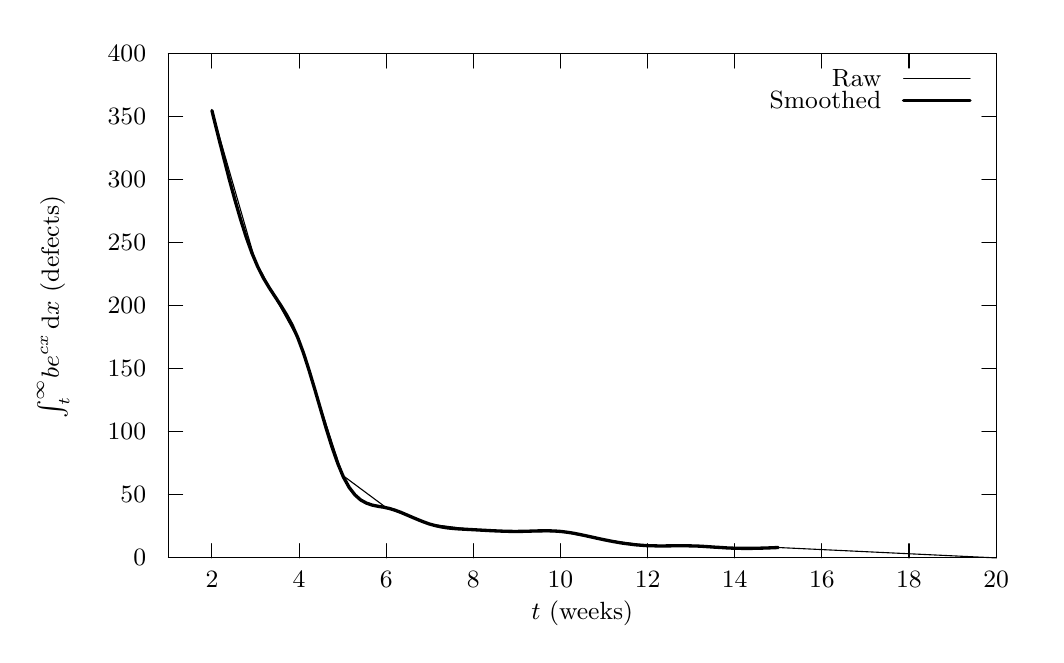
\begin{tikzpicture}[gnuplot]
%% generated with GNUPLOT 4.6p4 (Lua 5.1; terminal rev. 99, script rev. 100)
%% Thu 04 Sep 2014 10:50:27 WST
\tikzset{every node/.append style={font={\fontsize{9pt}{10.8pt}\selectfont}}}
\gpmonochromelines
\path (0.000,0.000) rectangle (12.700,7.620);
\gpcolor{color=gp lt color border}
\gpsetlinetype{gp lt border}
\gpsetlinewidth{1.00}
\draw[gp path] (1.688,0.886)--(1.868,0.886);
\draw[gp path] (12.201,0.886)--(12.021,0.886);
\node[gp node right] at (1.522,0.886) { 0};
\draw[gp path] (1.688,1.686)--(1.868,1.686);
\draw[gp path] (12.201,1.686)--(12.021,1.686);
\node[gp node right] at (1.522,1.686) { 50};
\draw[gp path] (1.688,2.486)--(1.868,2.486);
\draw[gp path] (12.201,2.486)--(12.021,2.486);
\node[gp node right] at (1.522,2.486) { 100};
\draw[gp path] (1.688,3.286)--(1.868,3.286);
\draw[gp path] (12.201,3.286)--(12.021,3.286);
\node[gp node right] at (1.522,3.286) { 150};
\draw[gp path] (1.688,4.087)--(1.868,4.087);
\draw[gp path] (12.201,4.087)--(12.021,4.087);
\node[gp node right] at (1.522,4.087) { 200};
\draw[gp path] (1.688,4.887)--(1.868,4.887);
\draw[gp path] (12.201,4.887)--(12.021,4.887);
\node[gp node right] at (1.522,4.887) { 250};
\draw[gp path] (1.688,5.687)--(1.868,5.687);
\draw[gp path] (12.201,5.687)--(12.021,5.687);
\node[gp node right] at (1.522,5.687) { 300};
\draw[gp path] (1.688,6.487)--(1.868,6.487);
\draw[gp path] (12.201,6.487)--(12.021,6.487);
\node[gp node right] at (1.522,6.487) { 350};
\draw[gp path] (1.688,7.287)--(1.868,7.287);
\draw[gp path] (12.201,7.287)--(12.021,7.287);
\node[gp node right] at (1.522,7.287) { 400};
\draw[gp path] (2.241,0.886)--(2.241,1.066);
\draw[gp path] (2.241,7.287)--(2.241,7.107);
\node[gp node center] at (2.241,0.609) { 2};
\draw[gp path] (3.348,0.886)--(3.348,1.066);
\draw[gp path] (3.348,7.287)--(3.348,7.107);
\node[gp node center] at (3.348,0.609) { 4};
\draw[gp path] (4.455,0.886)--(4.455,1.066);
\draw[gp path] (4.455,7.287)--(4.455,7.107);
\node[gp node center] at (4.455,0.609) { 6};
\draw[gp path] (5.561,0.886)--(5.561,1.066);
\draw[gp path] (5.561,7.287)--(5.561,7.107);
\node[gp node center] at (5.561,0.609) { 8};
\draw[gp path] (6.668,0.886)--(6.668,1.066);
\draw[gp path] (6.668,7.287)--(6.668,7.107);
\node[gp node center] at (6.668,0.609) { 10};
\draw[gp path] (7.774,0.886)--(7.774,1.066);
\draw[gp path] (7.774,7.287)--(7.774,7.107);
\node[gp node center] at (7.774,0.609) { 12};
\draw[gp path] (8.881,0.886)--(8.881,1.066);
\draw[gp path] (8.881,7.287)--(8.881,7.107);
\node[gp node center] at (8.881,0.609) { 14};
\draw[gp path] (9.988,0.886)--(9.988,1.066);
\draw[gp path] (9.988,7.287)--(9.988,7.107);
\node[gp node center] at (9.988,0.609) { 16};
\draw[gp path] (11.094,0.886)--(11.094,1.066);
\draw[gp path] (11.094,7.287)--(11.094,7.107);
\node[gp node center] at (11.094,0.609) { 18};
\draw[gp path] (12.201,0.886)--(12.201,1.066);
\draw[gp path] (12.201,7.287)--(12.201,7.107);
\node[gp node center] at (12.201,0.609) { 20};
\draw[gp path] (1.688,7.287)--(1.688,0.886)--(12.201,0.886)--(12.201,7.287)--cycle;
\node[gp node center,rotate=-270] at (0.221,4.086) {$\int_{t}^{\infty} \! be^{cx} \, \mathrm{d}x$ (defects)};
\node[gp node center] at (6.944,0.194) {$t$ (weeks)};
\node[gp node right] at (10.859,6.969) {Raw};
\gpcolor{color=gp lt color 3}
\gpsetlinetype{gp lt plot 3}
\draw[gp path] (11.025,6.969)--(11.869,6.969);
\draw[gp path] (2.241,6.568)--(2.795,4.647)--(3.348,3.642)--(3.901,1.935)--(4.455,1.524)%
  --(5.008,1.315)--(5.561,1.245)--(6.115,1.222)--(6.668,1.222)--(7.221,1.117)--(7.774,1.042)%
  --(8.328,1.039)--(8.881,1.009)--(9.434,1.018)--(12.201,0.886);
\gpcolor{color=gp lt color border}
\node[gp node right] at (10.859,6.692) {Smoothed};
\gpcolor{color=gp lt color 0}
\gpsetlinetype{gp lt plot 0}
\gpsetlinewidth{3.00}
\draw[gp path] (11.025,6.692)--(11.869,6.692);
\draw[gp path] (2.241,6.568)--(2.314,6.274)--(2.387,5.985)--(2.459,5.705)--(2.532,5.437)%
  --(2.605,5.187)--(2.677,4.959)--(2.750,4.756)--(2.823,4.584)--(2.895,4.441)--(2.968,4.319)%
  --(3.041,4.207)--(3.113,4.097)--(3.186,3.979)--(3.259,3.845)--(3.331,3.684)--(3.404,3.489)%
  --(3.476,3.265)--(3.549,3.022)--(3.622,2.772)--(3.694,2.525)--(3.767,2.292)--(3.840,2.084)%
  --(3.912,1.911)--(3.985,1.780)--(4.058,1.686)--(4.130,1.622)--(4.203,1.582)--(4.276,1.557)%
  --(4.348,1.542)--(4.421,1.530)--(4.494,1.514)--(4.566,1.492)--(4.639,1.465)--(4.712,1.434)%
  --(4.784,1.403)--(4.857,1.372)--(4.930,1.343)--(5.002,1.317)--(5.075,1.297)--(5.148,1.281)%
  --(5.220,1.269)--(5.293,1.261)--(5.366,1.255)--(5.438,1.251)--(5.511,1.247)--(5.584,1.243)%
  --(5.656,1.239)--(5.729,1.235)--(5.802,1.231)--(5.874,1.228)--(5.947,1.225)--(6.020,1.223)%
  --(6.092,1.222)--(6.165,1.223)--(6.237,1.224)--(6.310,1.227)--(6.383,1.229)--(6.455,1.230)%
  --(6.528,1.230)--(6.601,1.227)--(6.673,1.222)--(6.746,1.213)--(6.819,1.202)--(6.891,1.188)%
  --(6.964,1.173)--(7.037,1.157)--(7.109,1.141)--(7.182,1.125)--(7.255,1.110)--(7.327,1.096)%
  --(7.400,1.083)--(7.473,1.071)--(7.545,1.062)--(7.618,1.053)--(7.691,1.047)--(7.763,1.042)%
  --(7.836,1.040)--(7.909,1.038)--(7.981,1.038)--(8.054,1.039)--(8.127,1.040)--(8.199,1.040)%
  --(8.272,1.040)--(8.345,1.038)--(8.417,1.036)--(8.490,1.032)--(8.563,1.027)--(8.635,1.022)%
  --(8.708,1.018)--(8.781,1.013)--(8.853,1.010)--(8.926,1.008)--(8.998,1.007)--(9.071,1.007)%
  --(9.144,1.008)--(9.216,1.010)--(9.289,1.012)--(9.362,1.015)--(9.434,1.018);
\gpcolor{color=gp lt color border}
\gpsetlinetype{gp lt border}
\gpsetlinewidth{1.00}
\draw[gp path] (1.688,7.287)--(1.688,0.886)--(12.201,0.886)--(12.201,7.287)--cycle;
%% coordinates of the plot area
\gpdefrectangularnode{gp plot 1}{\pgfpoint{1.688cm}{0.886cm}}{\pgfpoint{12.201cm}{7.287cm}}
\end{tikzpicture}
%% gnuplot variables

    \caption{Scenario C Result}
  \end{figure}
  
  \begin{figure}[!htb]
    \centering
    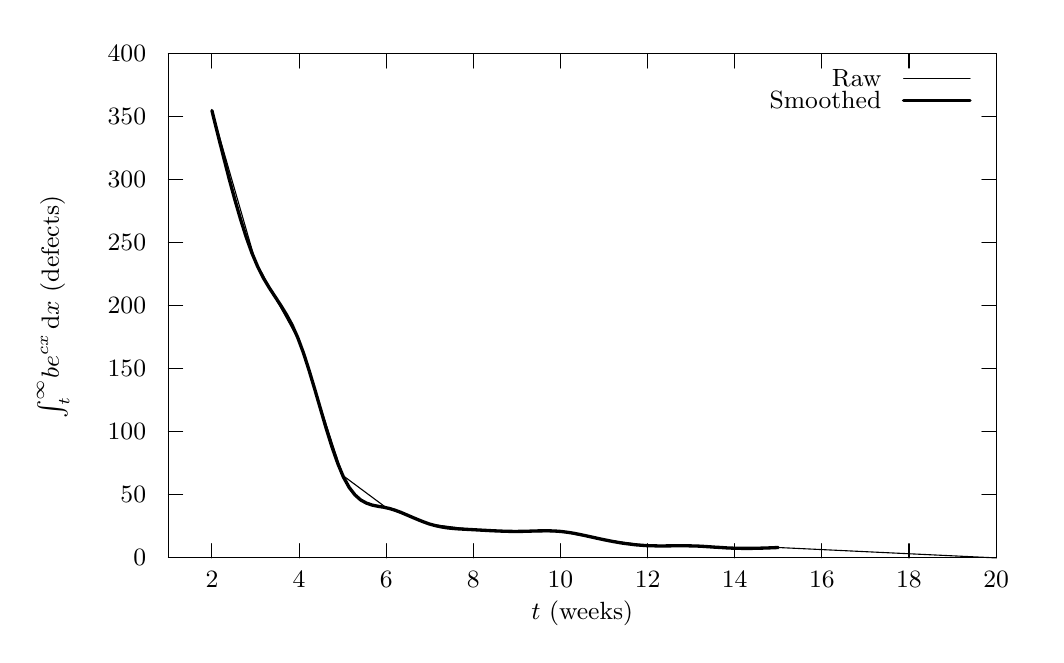
\begin{tikzpicture}[gnuplot]
%% generated with GNUPLOT 4.6p4 (Lua 5.1; terminal rev. 99, script rev. 100)
%% Thu 04 Sep 2014 10:50:27 WST
\tikzset{every node/.append style={font={\fontsize{9pt}{10.8pt}\selectfont}}}
\gpmonochromelines
\path (0.000,0.000) rectangle (12.700,7.620);
\gpcolor{color=gp lt color border}
\gpsetlinetype{gp lt border}
\gpsetlinewidth{1.00}
\draw[gp path] (1.688,0.886)--(1.868,0.886);
\draw[gp path] (12.201,0.886)--(12.021,0.886);
\node[gp node right] at (1.522,0.886) { 0};
\draw[gp path] (1.688,1.686)--(1.868,1.686);
\draw[gp path] (12.201,1.686)--(12.021,1.686);
\node[gp node right] at (1.522,1.686) { 50};
\draw[gp path] (1.688,2.486)--(1.868,2.486);
\draw[gp path] (12.201,2.486)--(12.021,2.486);
\node[gp node right] at (1.522,2.486) { 100};
\draw[gp path] (1.688,3.286)--(1.868,3.286);
\draw[gp path] (12.201,3.286)--(12.021,3.286);
\node[gp node right] at (1.522,3.286) { 150};
\draw[gp path] (1.688,4.087)--(1.868,4.087);
\draw[gp path] (12.201,4.087)--(12.021,4.087);
\node[gp node right] at (1.522,4.087) { 200};
\draw[gp path] (1.688,4.887)--(1.868,4.887);
\draw[gp path] (12.201,4.887)--(12.021,4.887);
\node[gp node right] at (1.522,4.887) { 250};
\draw[gp path] (1.688,5.687)--(1.868,5.687);
\draw[gp path] (12.201,5.687)--(12.021,5.687);
\node[gp node right] at (1.522,5.687) { 300};
\draw[gp path] (1.688,6.487)--(1.868,6.487);
\draw[gp path] (12.201,6.487)--(12.021,6.487);
\node[gp node right] at (1.522,6.487) { 350};
\draw[gp path] (1.688,7.287)--(1.868,7.287);
\draw[gp path] (12.201,7.287)--(12.021,7.287);
\node[gp node right] at (1.522,7.287) { 400};
\draw[gp path] (2.241,0.886)--(2.241,1.066);
\draw[gp path] (2.241,7.287)--(2.241,7.107);
\node[gp node center] at (2.241,0.609) { 2};
\draw[gp path] (3.348,0.886)--(3.348,1.066);
\draw[gp path] (3.348,7.287)--(3.348,7.107);
\node[gp node center] at (3.348,0.609) { 4};
\draw[gp path] (4.455,0.886)--(4.455,1.066);
\draw[gp path] (4.455,7.287)--(4.455,7.107);
\node[gp node center] at (4.455,0.609) { 6};
\draw[gp path] (5.561,0.886)--(5.561,1.066);
\draw[gp path] (5.561,7.287)--(5.561,7.107);
\node[gp node center] at (5.561,0.609) { 8};
\draw[gp path] (6.668,0.886)--(6.668,1.066);
\draw[gp path] (6.668,7.287)--(6.668,7.107);
\node[gp node center] at (6.668,0.609) { 10};
\draw[gp path] (7.774,0.886)--(7.774,1.066);
\draw[gp path] (7.774,7.287)--(7.774,7.107);
\node[gp node center] at (7.774,0.609) { 12};
\draw[gp path] (8.881,0.886)--(8.881,1.066);
\draw[gp path] (8.881,7.287)--(8.881,7.107);
\node[gp node center] at (8.881,0.609) { 14};
\draw[gp path] (9.988,0.886)--(9.988,1.066);
\draw[gp path] (9.988,7.287)--(9.988,7.107);
\node[gp node center] at (9.988,0.609) { 16};
\draw[gp path] (11.094,0.886)--(11.094,1.066);
\draw[gp path] (11.094,7.287)--(11.094,7.107);
\node[gp node center] at (11.094,0.609) { 18};
\draw[gp path] (12.201,0.886)--(12.201,1.066);
\draw[gp path] (12.201,7.287)--(12.201,7.107);
\node[gp node center] at (12.201,0.609) { 20};
\draw[gp path] (1.688,7.287)--(1.688,0.886)--(12.201,0.886)--(12.201,7.287)--cycle;
\node[gp node center,rotate=-270] at (0.221,4.086) {$\int_{t}^{\infty} \! be^{cx} \, \mathrm{d}x$ (defects)};
\node[gp node center] at (6.944,0.194) {$t$ (weeks)};
\node[gp node right] at (10.859,6.969) {Raw};
\gpcolor{color=gp lt color 3}
\gpsetlinetype{gp lt plot 3}
\draw[gp path] (11.025,6.969)--(11.869,6.969);
\draw[gp path] (2.241,6.568)--(2.795,4.647)--(3.348,3.642)--(3.901,1.935)--(4.455,1.524)%
  --(5.008,1.315)--(5.561,1.245)--(6.115,1.222)--(6.668,1.222)--(7.221,1.117)--(7.774,1.042)%
  --(8.328,1.039)--(8.881,1.009)--(9.434,1.018)--(12.201,0.886);
\gpcolor{color=gp lt color border}
\node[gp node right] at (10.859,6.692) {Smoothed};
\gpcolor{color=gp lt color 0}
\gpsetlinetype{gp lt plot 0}
\gpsetlinewidth{3.00}
\draw[gp path] (11.025,6.692)--(11.869,6.692);
\draw[gp path] (2.241,6.568)--(2.314,6.274)--(2.387,5.985)--(2.459,5.705)--(2.532,5.437)%
  --(2.605,5.187)--(2.677,4.959)--(2.750,4.756)--(2.823,4.584)--(2.895,4.441)--(2.968,4.319)%
  --(3.041,4.207)--(3.113,4.097)--(3.186,3.979)--(3.259,3.845)--(3.331,3.684)--(3.404,3.489)%
  --(3.476,3.265)--(3.549,3.022)--(3.622,2.772)--(3.694,2.525)--(3.767,2.292)--(3.840,2.084)%
  --(3.912,1.911)--(3.985,1.780)--(4.058,1.686)--(4.130,1.622)--(4.203,1.582)--(4.276,1.557)%
  --(4.348,1.542)--(4.421,1.530)--(4.494,1.514)--(4.566,1.492)--(4.639,1.465)--(4.712,1.434)%
  --(4.784,1.403)--(4.857,1.372)--(4.930,1.343)--(5.002,1.317)--(5.075,1.297)--(5.148,1.281)%
  --(5.220,1.269)--(5.293,1.261)--(5.366,1.255)--(5.438,1.251)--(5.511,1.247)--(5.584,1.243)%
  --(5.656,1.239)--(5.729,1.235)--(5.802,1.231)--(5.874,1.228)--(5.947,1.225)--(6.020,1.223)%
  --(6.092,1.222)--(6.165,1.223)--(6.237,1.224)--(6.310,1.227)--(6.383,1.229)--(6.455,1.230)%
  --(6.528,1.230)--(6.601,1.227)--(6.673,1.222)--(6.746,1.213)--(6.819,1.202)--(6.891,1.188)%
  --(6.964,1.173)--(7.037,1.157)--(7.109,1.141)--(7.182,1.125)--(7.255,1.110)--(7.327,1.096)%
  --(7.400,1.083)--(7.473,1.071)--(7.545,1.062)--(7.618,1.053)--(7.691,1.047)--(7.763,1.042)%
  --(7.836,1.040)--(7.909,1.038)--(7.981,1.038)--(8.054,1.039)--(8.127,1.040)--(8.199,1.040)%
  --(8.272,1.040)--(8.345,1.038)--(8.417,1.036)--(8.490,1.032)--(8.563,1.027)--(8.635,1.022)%
  --(8.708,1.018)--(8.781,1.013)--(8.853,1.010)--(8.926,1.008)--(8.998,1.007)--(9.071,1.007)%
  --(9.144,1.008)--(9.216,1.010)--(9.289,1.012)--(9.362,1.015)--(9.434,1.018);
\gpcolor{color=gp lt color border}
\gpsetlinetype{gp lt border}
\gpsetlinewidth{1.00}
\draw[gp path] (1.688,7.287)--(1.688,0.886)--(12.201,0.886)--(12.201,7.287)--cycle;
%% coordinates of the plot area
\gpdefrectangularnode{gp plot 1}{\pgfpoint{1.688cm}{0.886cm}}{\pgfpoint{12.201cm}{7.287cm}}
\end{tikzpicture}
%% gnuplot variables

    \caption{Scenario D Result}
  \end{figure}

  
\end{appendices}

\end{document}
